
\documentclass {article}

\setlength {\textwidth} {6in}
\setlength {\textheight} {8in}
\setlength {\topmargin} {0in}
\setlength {\oddsidemargin} {0.25in}
\setlength {\evensidemargin} {0.25in}
\addtolength {\parskip} {1ex}

\newcommand {\caps}[1] {\mbox {\ifnum\fam=0 \scshape\else\uppercase\fi{#1}}}

\newcommand {\tdadvisor} {Theses and Dissertations Advisor}
\newcommand {\csd} {Computer Science Department}
\newcommand {\regs} {{\sl Regulations for Thesis
		      and Dissertation Preparation}}
\newcommand {\ucla} {\caps {ucla}}
\newcommand {\uclacsd} {\ucla\ \csd}
\newcommand {\umi} {\caps {umi}}

\title	{ Formatting UCLA Theses and Dissertations \\
	 Using \LaTeX \\
	 and the \texttt{uclathes} Document Style}
\author {Rich Wales}
\date{}
\begin {document}
\maketitle

\newcommand{\MaintainNote}[1]{{\slshape Maintainer's note:  #1}}

\MaintainNote{
  This document was written by Rich Wales for his \texttt{thesis} style.
  I've updated it for the \texttt{uclathes} style for \LaTeX 2e.
  Typos are probably mine.
   ---John Heidemann.}


This document explains how to format your thesis%
\footnote {In order not to make this document overly verbose,
the term {\em thesis\/} will be used throughout
to indicate either a ``thesis'' (master's degree document)
or a ``dissertation'' (doctor's degree document).
The formatting requirements, in any case,
are virtually identical for both theses and dissertations.
Ph.D.\ students should understand that---%
unless indicated otherwise---%
anything said here about a {\em thesis\/}
applies with equal force to a {\em dissertation\/} as well.}
manuscript using \LaTeX.
It describes a special ``document style'' macro package
which, it is believed, will meet \ucla's requirements
regarding type size, layout, spacing, and margins.

These instructions are not intended to replace
the \ucla\ Graduate Division's publication, \regs.
All graduate students should obtain a copy of this publication,
read it carefully, and check again in advance
of the filing deadline to see if any changes have been made
to the requirements.


\section {Thesis and Dissertation Format Requirements}

Theses filed at \ucla\ are required to conform
to certain physical format specifications.
Among the reasons why such formatting issues are important
are the following:

\begin {itemize}

\item
Theses are public, published documents.
A copy of every thesis produced at \ucla\
is filed in one or more University libraries,
and are also available on microfilm
to researchers elsewhere.

Each thesis manuscript is a reflection
of the high standards of the University.
A sloppy manuscript makes the University itself look sloppy,
and so such manuscripts cannot be accepted for filing.

\item
Theses are microfilmed for archival purposes.
Additionally, doctoral dissertations are generally
microfilmed as well by University Microfilms International (\umi).
In order to ensure that the manuscript
will reproduce properly on microfilm,
it is important that the type face is sufficiently large
and that the strokes of the letters are not excessively thin.

\item
In order to guarantee successful binding
of a thesis manuscript in book form---%
as well as to ensure problem-free microfilming---%
the text margins and page number placement
must conform to known standards.

\item
Page numbering must be done in a standardized, consistent fashion,
so as to ensure that errors (such as missed pages)
will not occur in either the binding or the microfilming process.

\end {itemize}

It is crucial that a thesis manuscript
should conform to the University's formatting requirements.
A non-conforming manuscript will \emph{not} be accepted for filing---%
even if the content has been approved
by the student's committee;
even if (in the case of a problem with the signature page)
one or more committee members are not available to sign again;
and even if not enough time remains for the student
to redo the manuscript and file a satisfactory copy by the deadline.
You snooze, you loose.

In order to avoid last-minute disasters,
the \ucla\ \tdadvisor\ strongly urges \emph{all} graduate students
to submit a sample of their thesis manuscript
(including all the preliminary pages)
for review and approval well in advance of the filing deadline.
Think about how long you've been here---can't you really 
  manage to get that dissertation to Powell slightly before the
  last day to file?


\section {Using the \LaTeX\ \texttt{uclathes} Style}

This section describes how to set up
the \LaTeX\ input for your thesis
to use the \verb|uclathes| document style macros.

\subsection {Overall \LaTeX\ Source File Format}

Following are two sample \LaTeX\ input files
which illustrate the proper use of the \verb+uclathes+
document style.

Figure~\ref{fig:toplevel}
shows a ``top-level'' input file,
which itself contains only a minimal skeleton
and includes text from other files
via \verb+\input+ commands.
Figures~\ref{fig:prelim1} and \ref{fig:prelim2}
show the commands for setting up the preliminary pages.

\subsection {The $\backslash${\tt documentclass} Command}

The \verb+\documentclass+ command at the start of the \LaTeX\ input text
should have the following form:

\begin {center}
\verb+\documentclass [+{\sl options\/}\verb+] {uclathes}+
\end {center}

where {\sl options} is one of the following:

\begin {description}

\item [{\tt MS}]
--- M.S.\ thesis.

\item [{\tt PhD}]
--- Ph.D.\ dissertation.

\end {description}

Note that capitalization is important:
\verb+ms+, \verb+PHD+, or \verb+phd+ will {\em not\/} work.

The \verb+uclathes+ document style is basically the same
as the standard \LaTeX\ \verb+report+ style,
as far as the body of the text is concerned.

\subsection {The $\backslash${\tt bibliographystyle} Command}

There is a matching \verb+uclathes+ bibliography style
which should be used in conjunction with
the \verb+uclathes+ document style.
To use the \verb+uclathes+ bibliography style,
use the following \verb+\bibliographystyle+ command
near the end of your \LaTeX\ input
(just before the \verb+\end {document}+ command):

\begin {center} \verb+\bibliographystyle {uclathes}+ \end {center}

The \verb+uclathes+ bibliography style is similar to the
standard Bib\TeX\ \verb+alpha+ style.
One important new feature in the \verb+uclathes+ style is
the addition of a new \verb+annote+ field in a reference,
which can be used to produce an annotated bibliography.

\begin {figure}
{\small
\begin{verbatim}
\documentclass [PhD] {uclathes}
\usepackage{tikz}
\usetikzlibrary{positioning}
\usetikzlibrary{calc}


\usepackage{enumitem}  
\usepackage{mathrsfs} 

\newcommand{\X}{\mathcal X}
\newcommand{\Y}{\mathcal Y}


\DeclareMathOperator{\TT}{\mathcal T}
\DeclareMathOperator{\PR}{P}
\DeclareMathOperator{\cl}{cl}
\newcommand{\CS}{\mathcal S}

\DeclareMathOperator{\cx}{Complexity}
\newcommand{\K}{\boldface K_\alpha}
\renewcommand{\S}{S_\alpha}

\DeclareMathOperator{\I}{\mathcal I}
\DeclareMathOperator{\J}{\mathcal J}
\DeclareMathOperator{\acl}{acl}
\DeclareMathOperator{\Aut}{Aut}

\renewcommand{\SS}{\mathbb S}


\renewcommand{\AA}{\mathscr A}
\newcommand{\BB}{\mathscr B}
\newcommand{\DD}{\mathscr D}
\newcommand{\II}{\mathscr I}
\newcommand{\MM}{\mathbb M}

\newcommand{\A}{\mathcal A}
\newcommand{\B}{\mathcal B} 
\renewcommand{\C}{\mathcal C}
\newcommand{\D}{\mathcal D}
\newcommand{\F}{\mathcal F}
\newcommand{\G}{\mathcal G}
\renewcommand{\H}{\mathcal H}
\renewcommand{\LL}{\mathcal L}
\newcommand{\LLA}{\mathcal L_{aff}}
\newcommand{\LLM}{\mathcal L_{Mac}}
\newcommand{\M}{\mathcal M}

\newcommand{\U}{\mathcal U}	

\DeclareMathOperator{\Sg}{Sg}
\DeclareMathOperator{\It}{Tp}
\DeclareMathOperator{\Sub}{Sub}
\DeclareMathOperator{\Ct}{Ct}
\DeclareMathOperator{\vecspan}{span}
\DeclareMathOperator{\val}{val}
\DeclareMathOperator{\vval}{val}
\DeclareMathOperator{\tval}{T-val}
\DeclareMathOperator{\tfl}{T-fl}
\DeclareMathOperator{\inti}{I}

\newcommand{\interval}{\inti(t, \alpha_L, \alpha_U)}

\newcommand{\GG}{\mathbb G}
\newcommand{\GGY}{\GG^{|y|}}
\newcommand{\AX}{A^{|x|}}
\newcommand{\BA}{\bar A}

\DeclareMathOperator{\diag}{diag}

\newcommand{\DB}{\mathbb D}
\newcommand{\ppp}{\partial}
\newcommand{\BM}{\bar M_{j-1}}
\newcommand{\E}{\mathscr E}
\DeclareMathOperator{\ind}{ind}
\newcommand{\vcind}{\vc_{\ind}}
\newcommand{\Ind}{\mathscr I}


\newcommand{\curly}[1]{\left\{#1\right\}}
\newcommand{\paren}[1]{\left(#1\right)}
\newcommand{\abs}[1]{\left|#1\right|}
\newcommand{\agl}[1]{\left\langle #1 \right\rangle}

\providecommand{\floor}[1]{\left \lfloor #1 \right \rfloor }

\usepackage{soul}
\newcommand{\defn}{\ul}

%\newenvironment{openq}{\paragraph{Open Question:}}{}
\renewcommand{\subset}{\subseteq}

\DeclareMathOperator{\TTB}{\boldface T}
\DeclareMathOperator{\AT}{\boldface A}
\DeclareMathOperator{\BT}{\boldface B}


\newcommand{\LLU}{\LL^*}


                         % personal LaTeX macros
\input {prelim}                           % preliminary page info
\begin {document}
\makeintropages
\input {chapter1}                         % Chapter 1 of dissertation

%
% introduction.tex
% Copyright (C) 1995 by John Heidemann, <johnh@isi.edu>.
% $Id: demo2intr.tex,v 1.1 1996/01/12 18:13:58 johnh Exp $
%

\chapter{Non-tracial transport}\label{non-tracial transport chapter}

%%%%%%%%%%%%%%%%%%%%%%%%
%                 		Preliminaries	          		          %
%%%%%%%%%%%%%%%%%%%%%%%%

\section{Preliminaries}\label{prelim}



%	The free Araki-Woods factor and $q$-deformed Araki-Woods algebras
%%%%%%%%%%%%%%%%%%%%%%%%%%%%%%%%%%%%%%%%%%%%%
\subsection{The free Araki-Woods factor and $q$-deformed Araki-Woods algebras}\label{free_Araki-Woods}

Let $\H_\R$ be a real Hilbert space and $U_t$ a strongly continuous one-parameter group of orthogonal transformations on $\H_\R$. Letting $\H_\C:=\H_\R +\i \H_\R$ be the complexified Hilbert space, the $U_t$ can be extended to a one-parameter unitary group (still denoted as $U_t$). Let $A$ be the generator of the $U_t$ (i.e. $U_t=A^{it}$ and $A$ is a potentially unbounded positive operator). Let $\<\cdot,\cdot\>$ be the inner product on $\H_\C$ which is complex-linear in the second coordinate (as all other inner products will be in this section). Define an inner product $\<\cdot,\cdot\>_U$ on $\H_\C$ by
	\begin{align*}
		\<x,y\>_U  = \< \frac{2}{1+A^{-1}}x, y\>,\qquad x,y\in\H_\C.
	\end{align*}
Let $\H$ be the complex Hilbert space obtained by completing $\H_\C$ with respect to $\<\cdot,\cdot\>_U$. Note that if we start with the trivial one-parameter group $U_t=1$ for all $t$ then $A=1$, $\<\cdot,\cdot\>_U=\<\cdot,\cdot\>$ and $\H=\H_\C$. In this case we will write $\<\cdot,\cdot\>_1$ for $\<\cdot,\cdot\>_U$.\par
For $-1<q<1$, the $q$-Fock space $\mathcal{F}_q(\H)$ is the completion of $\mathcal{F}^{\text{finite}}(\H):=\bigoplus_{n=0}^\infty \H^{\otimes n}$, where $\H^{\otimes 0}=\C\Omega$ with vacuum vector $\Omega$, with respect to the sesquilinear form $\<\cdot,\cdot\>_{U,q}$ given by
	\begin{align*}
		\<f_1\otimes\cdots\otimes f_n, g_1\otimes\cdot\otimes g_m\>_{U,q} = \delta_{n=m} \sum_{\pi\in S_n} q^{i(\pi)} \<f_1,g_{\pi(1)}\>_U\cdots \<f_n,g_{\pi(n)}\>_U,
	\end{align*}
where $i(\pi)$ denotes the number of inversions of the permutation $\pi\in S_n$. We may at times denote $\mathcal{F}_q(\H_\R,U_t)=\mathcal{F}_q(\H)$ to emphasize $\{U_t\}$.

For any $h\in \H$ we can define the left $q$-creation operator $l(h)\in \B(\mc{F}_q(\H))$ by
	\begin{align*}
		&l_q(h)\Omega=h;\\
		&l_q(h)(f_1\otimes\cdots\otimes f_n)=h\otimes f_1\otimes\cdots \otimes f_n,
	\end{align*}
then its adjoint is the left $q$-annihilation operator:
	\begin{align*}
		&l_q^*(h)\Omega=0;\\
		&l_q^*(h)(f_1\otimes\cdots\otimes f_n)= \sum_{i=1}^n q^{i-1} \<h,f_i\>_U f_1\otimes \cdots \otimes f_{i-1}\otimes f_{i+1}\otimes\cdots \otimes f_n.
	\end{align*}
Also define
	\begin{align*}
		s_q(h):=l_q(h)+l_q^*(h).
	\end{align*}\par
We let $\Gamma_q(\H_\R,U_t)$ be the $C^*$-algebra generated by $\{s_q(h)\colon h\in\H_\R\}$. The corresponding von Neumann algebra $M_q:=\Gamma_q(\H_\R,U_t)''\subset \B(\mc{F}_q(\H))$ is called a \emph{$q$-deformed Araki-Woods algebra}, after \cite{Hia03}, except when $q=0$ where $M_0=\Gamma_0(\H_\R,U_t)''$ is called a \emph{free Araki-Woods factor}, after \cite{Shl97}.\par
It was shown in \cite{Hia03} that $\Omega$ is a cyclic and separating vector for $M_q$ and consequently the vacuum state $\varphi_q(\cdot)=\<\Omega,\cdot\  \Omega\>_{U,q}$ is faithful. For $q\neq 0$, $\varphi_q$ is called the \emph{$q$-quasi-free state}, or the \emph{$q$-quasi-free state associated to $A$}. For $q=0$, $\varphi_0$ is called the \emph{free quasi-free state}, or the \emph{free quasi-free state associated to $A$}.\par

\begin{rem}
For $f_1,\ldots, f_n\in \H_\R$, computing $\varphi_q(s_q(f_1)\cdots s_q(f_n))$ is best done diagrammatically through non-crossing (when $q=0$) and crossing (when $q\neq 0$) pairing diagrams. When $q=0$, visualize a rectangle with the vectors $f_1,\ldots, f_n$ arranged in order along the top:
	\begin{equation*}
		\begin{tikzpicture}
			\draw [thick] (0,0) -- (0,0.6) -- (2.2,0.6) -- (2.2,0) -- (0,0);
			\node at (1.1,0.3) {$f_1\ f_2\ \cdots\ f_n$};
		\end{tikzpicture}.
	\end{equation*}
$\varphi(s(f_1)\cdots s(f_n))$ counts all the ways to pair the vectors to each other via chords above the rectangle so that no two chords intersect and if a vector $f_i$ is connected to a vector $f_j$ (with $f_i$ on the left) then that diagram is weighted by a factor of $\<f_i,f_j\>_U$. For example the following diagram has the denoted weight:
	\begin{equation*}
		\begin{tikzpicture}[baseline]
			\draw [thick] (0,0.3) -- (0,-0.3) -- (3.6,-0.3) -- (3.6,0.3) -- (0,0.3);
			\node at (.3,0) {$f_1$};
			\node at (.9,0) {$f_2$};
			\node at (1.5,0) {$f_3$};
			\node at (2.1,0) {$f_4$};
			\node at (2.7,0) {$f_5$};
			\node at (3.3,0) {$f_6$};
			\draw[thick] (2.1,0.3) arc (0:180:0.9 and 0.6); %coordinate marks the right end-point of the semi-circle NOT the center
			\draw[thick] (1.5,0.3) arc (0:180:0.3 and 0.2);
			\draw[thick] (3.3,0.3) arc (0:180:0.3 and 0.2);
		\end{tikzpicture}
		=\<f_1,f_4\>_U\<f_2,f_3\>_U\<f_5,f_6\>_U.
	\end{equation*}
Thus
	\begin{align*}
		\varphi(s(f_1)s(f_2)s(f_3)s(f_4)) &= 
			\begin{tikzpicture}[baseline]
			\draw [thick] (0,0.3) -- (0,-0.3) -- (2.4,-0.3) -- (2.4,0.3) -- (0,0.3);
			\node at (.3,0) {$f_1$};
			\node at (.9,0) {$f_2$};
			\node at (1.5,0) {$f_3$};
			\node at (2.1,0) {$f_4$};
			\draw[thick] (0.9,0.3) arc (0:180:0.3 and 0.2);
			\draw[thick] (2.1,0.3) arc (0:180:0.3 and 0.2);
			\end{tikzpicture}
		+
			\begin{tikzpicture}[baseline]
			\draw [thick] (0,0.3) -- (0,-0.3) -- (2.4,-0.3) -- (2.4,0.3) -- (0,0.3);
			\node at (.3,0) {$f_1$};
			\node at (.9,0) {$f_2$};
			\node at (1.5,0) {$f_3$};
			\node at (2.1,0) {$f_4$};
			\draw[thick] (2.1,0.3) arc (0:180:0.9 and 0.6);
			\draw[thick] (1.5,0.3) arc (0:180:0.3 and 0.2);
			\end{tikzpicture}\\
		&=\<f_1,f_2\>_U\<f_3,f_4\>_U + \<f_1, f_4\>_U\<f_2,f_3\>_U.
	\end{align*}
Note that $\varphi$ then clearly takes a value of zero on all monomials of odd degree.\par
When $q\neq 0$, the chords may intersect and do so at the cost of a factor of $q$ for each intersection. Revisiting the previous example in this case we then have
	\begin{align*}
		\varphi_q(s_q(f_1)s_q(f_2)s_q(f_3)s_q(f_4)) &= 
			\begin{tikzpicture}[baseline]
			\draw [thick] (0,0.3) -- (0,-0.3) -- (2.4,-0.3) -- (2.4,0.3) -- (0,0.3);
			\node at (.3,0) {$f_1$};
			\node at (.9,0) {$f_2$};
			\node at (1.5,0) {$f_3$};
			\node at (2.1,0) {$f_4$};
			\draw[thick] (0.9,0.3) arc (0:180:0.3 and 0.2);
			\draw[thick] (2.1,0.3) arc (0:180:0.3 and 0.2);
			\end{tikzpicture}
		+
			\begin{tikzpicture}[baseline]
			\draw [thick] (0,0.3) -- (0,-0.3) -- (2.4,-0.3) -- (2.4,0.3) -- (0,0.3);
			\node at (.3,0) {$f_1$};
			\node at (.9,0) {$f_2$};
			\node at (1.5,0) {$f_3$};
			\node at (2.1,0) {$f_4$};
			\draw[thick] (1.5,0.3) arc (0:180:0.6 and 0.4);
			\draw[thick] (2.1,0.3) arc (0:180:0.6 and 0.4);
			\end{tikzpicture}
		+
			\begin{tikzpicture}[baseline]
			\draw [thick] (0,0.3) -- (0,-0.3) -- (2.4,-0.3) -- (2.4,0.3) -- (0,0.3);
			\node at (.3,0) {$f_1$};
			\node at (.9,0) {$f_2$};
			\node at (1.5,0) {$f_3$};
			\node at (2.1,0) {$f_4$};
			\draw[thick] (2.1,0.3) arc (0:180:0.9 and 0.6);
			\draw[thick] (1.5,0.3) arc (0:180:0.3 and 0.2);
			\end{tikzpicture}\\
		&=\<f_1,f_2\>_U\<f_3,f_4\>_U + q\<f_1,f_3\>_U\<f_2,f_4\>_U + \<f_1, f_4\>_U\<f_2,f_3\>_U.
	\end{align*}
We note that in computing $\varphi_q(s_q(f_1)s_q(f_2)s_q(f_3)s_q(f_4))=\<\Omega, s_q(f_1)s_q(f_2)s_q(f_3)s_q(f_4)\Omega\>_{U,q}$ by writing out $s_q(f_1)s_q(f_2)s_q(f_3)s_q(f_4)\Omega$, the term $ q\<f_1,f_3\>_U\<f_2,f_4\>_U$ comes from when $s_q(f_1)s_q(f_2)$ acts on $f_3\otimes f_4$ and the operator $l_q^*(f_2)$ ``skips'' over the the first vector in the tensor product (hence the factor of $q$).\par
It is a worthwhile exercise to restrict to the case when there is only a single operator $s_q(f)$ (so that all inner-products are $1$) and draw out the diagrams corresponding to $\varphi(s_q(f)^n)$ for $n=2,4,6,8$.
\end{rem}

The Tomita-Takesaki theory for $M_q$ is established in Lemma 1.4 of \cite{Hia03}, which we recall here for convenience. Let $S$ denote the closure of the map $x\Omega\mapsto x^*\Omega$, and let $S=J\Delta^{1/2}$ be its polar decomposition so that $J$ and $\Delta$ are the modular conjugation and modular operator, respectively. Then for $n\geq 1$
	\begin{align}\label{Tomita-Takesaki_formulas}
		S(f_1\otimes\cdots\otimes f_n)&=f_n\otimes \cdots \otimes f_n	&\text{for }f_1,\ldots, f_n\in\H_\R;\notag\\
		\Delta(f_1\otimes\cdots\otimes f_n)&=(A^{-1}f_1)\otimes \cdots\otimes (A^{-1} f_n)		&\text{for }f_1,\ldots,f_n\in \H_\R\cap \text{dom}{A^{-1}};\\
		J(f_1\otimes\cdots\otimes f_n)&=(A^{-1/2} f_n)\otimes\cdots \otimes (A^{-1/2}f_n)		&\text{for }f_1,\ldots, f_n\in \H_\R\cap\text{dom}{A^{-1/2}}.\notag
	\end{align}
Denote by $\sigma_t^{\varphi_q}(\cdot)= \Delta^{it} \cdot \Delta^{-it}$ the modular automorphism group of $\varphi_q$.\par
Henceforth we assume $\dim(\H_\R)=N<\infty$. Consequently $A$ and $A^{-1}$ are bounded operators and hence $\{\sigma_t^{\varphi_q}\}_{t\in\R}$ extends to $\{\sigma_z^{\varphi_q}\}_{z\in\C}$. In particular for $a,b\in M$,
	\begin{align*}
		\varphi(ab)&=\< a^*\Omega, b\Omega\>_{U,q}=\< S a\Omega, b\Omega\>_{U,q}=\<Jb\Omega, \Delta^\frac{1}{2} a\Omega\>_{U,q}\\
				&=\< \Delta \Delta^{-\frac{1}{2}} Jb\Omega,a\Omega\>_{U,q} = \< \Delta b^*\Omega, a\Omega\>_{U,q}= \varphi(\sigma_{i}^{\varphi_q}(b) a).
	\end{align*}
Moreover, the action of $\Delta$ in (\ref{Tomita-Takesaki_formulas}) extends to $f_1,\ldots, f_n\in \H$.\par
From Remark 2.12 in \cite{Shl97} it follows that for a suitable orthonormal basis $\{e_1,\ldots,e_N\}$ of $(\H_\R,\<\cdot,\cdot\>)$, the generator $A$ can be represented as a matrix of the form
	\begin{equation}\label{matrix_form_A}
		A=\text{diag}\left( A_1,\ldots, A_L,1,\ldots,1\right),
	\end{equation}
where for each $k\in\{1,\ldots,L\}$
	\begin{equation}\label{matrix_form_A_2}
		A_k=\frac{1}{2}\left(\begin{array}{cc}
						\lambda_k+\lambda_k^{-1}		& -i\left(\lambda_k-\lambda_k^{-1}\right)	\\
						i\left(\lambda_k-\lambda_k^{-1}\right)	& \lambda_k+\lambda_k^{-1}	\end{array}\right)\in M_2(\C),
	\end{equation}
and $\lambda_k>0$. Note that
	\begin{equation*}
		A_k^{it}=\left(\begin{array}{cc}	\cos(t\log{\lambda_k})	&	-\sin(t\log{\lambda_k})\\
								\sin(t\log{\lambda_k}) 	& 	\cos(t\log{\lambda_k})\end{array}\right),
	\end{equation*}
which is a unitary matrix such that $(A_k^{it})^*=(A_k^{it})^\text{T}=A_k^{-it}$. $A$ has the following properties:
	\begin{enumerate}
		\item[1.] $\text{spectrum}(A)=\left\{1,\lambda_1^{\pm 1},\ldots, \lambda_L^{\pm 1}\right\}$;
		\item[2.] $A^\text{T}=A^{-1}$;
		\item[3.] $\left( A^{it}\right)^*=\left( A^{it}\right)^\text{T}=A^{-it}$; and
		\item[4.] for any fixed $i\in\{1,\ldots, N\}$, 
			\begin{equation*}
				\sum_{j=1}^N \left|[A]_{ij}\right|\leq \max\left\{1,\lambda_1^{\pm 1},\ldots, \lambda_L^{\pm 1}\right\}\leq \|A\|.
			\end{equation*}
	\end{enumerate}
For each $j=1,\ldots, N$, let $X_j^{(q)}=s_q(e_j)$ and write $X^{(q)}=(X_1^{(q)},\ldots, X_N^{(q)})$. Since $s_q$ is real linear, it follows that $M_q=W^*(X_1^{(q)},\ldots, X_N^{(q)})$. We observe that
	\begin{align*}
		\sigma_z^{\varphi_q}(X_j^{(q)})=\sum_{k=1}^N [A^{iz}]_{jk} X_k^{(q)},\qquad \forall z\in \C,
	\end{align*}
or using the vector notation:
	\begin{align}\label{modular_semicircular}
		\sigma_z^{\varphi_q}(X^{(q)})= A^{iz} X^{(q)},\qquad \forall z\in\C.
	\end{align}
Indeed, using (\ref{Tomita-Takesaki_formulas}) it is easy to see that
	\begin{align*}
		\sigma_z^{\varphi_q}(l_q(e_j))&= l_q(A^{-iz} e_j)\\
		\sigma_z^{\varphi_q}(l_q^*(e_j))&=l_q^*( A^{-i\bar{z}} e_j).
	\end{align*}
Equation (\ref{modular_semicircular}) follows from the above properties of $A$, the linearity of $l_q$, and the conjugate linearity of $l_q^*$.


%	Derviations on $M_q$
%%%%%%%%%%%%%%%%%%%%%%%%%%%%%%%%%%%%%%%%
\subsection{Derivations on $M_q$}\label{derivations_on_M_q}

For the remainder of this section we will consider a single fixed $q\in (-1,1)$, so that we may repress the superscript $(q)$ notation on $X^{(q)}_j$, and write $\mathscr{P}$ for the $*$-subalgebra $\C\<X_1,\ldots, X_N\>\subset M_q$ of non-commutative polynomials in $N$-variables. We also simplify notation with $M:=M_q$, $\varphi:=\varphi_q$, and $\sigma_z:=\sigma_z^{\varphi_q}$ for $z\in \C$.\par
For each $j\in\{1,\ldots,N\}$ we let $\delta_j\colon \mathscr{P}\rightarrow \mathscr{P}\otimes\mathscr{P}^{op}$ be Voiculescu's free-difference quotient:
	\begin{align*}
		\delta_j(X_{i_1}\cdots X_{i_n})=\sum_{k=1}^n \delta_{j=i_k} X_{i_1}\cdots X_{i_{k-1}}\otimes \left(X_{i_{k+1}}\cdots X_{i_n}\right)^\circ;
	\end{align*}
that is, $\delta_j$ is the unique derivation satisfying $\delta_j(X_i)=\delta_{j=i}1\otimes 1$. We set the following conventions for working with elementary tensors in $\mathscr{P}\otimes\mathscr{P}^{op}$:
	\begin{itemize}
		\item $(a\otimes b^\circ)\#(c\otimes d^\circ):= (ac)\otimes (b^\circ d^\circ)=(ac)\otimes (db)^\circ$;
		\item $(a\otimes b^\circ)\#c=acb$;
		\item $(a\otimes b^\circ)^*:=a^*\otimes (b^*)^\circ$;
		\item $(a\otimes b^\circ)^\dagger:= b^*\otimes (a^*)^\circ$;
		\item $(a\otimes b^\circ)^\diamond:= b\otimes a^\circ$;
		\item $m(a\otimes b^\circ):=ab$.
	\end{itemize}
We also define the left and right actions of $\mathscr{P}$ as:
	\begin{itemize}
		\item $c\cdot (a\otimes b^\circ):=(ca)\otimes b^\circ$;
		\item $(a\otimes b^\circ)\cdot c:=a\otimes (bc)^\circ$.
	\end{itemize}
Note that 
	\begin{align*}
		c\cdot (a\otimes b^\circ)&= (c\otimes 1^\circ)\# (a\otimes b^\circ),\ \text{and}\\
		(a\otimes b^\circ)\cdot c &= (1\otimes c^\circ )\# (a\otimes b^\circ).
	\end{align*}
We will usually suppress the notation ``$\circ$" and at times represent tensors  of monomials in $\mathscr{P}$ diagrammatically as follows:
	\begin{align}\label{box_notation}
	\begin{tikzpicture}[baseline]
	\draw[thick] (0,-.5) rectangle (2.5,.5);
	\node[left] at (0,0) {$X_{i_1}\cdots X_{i_n}\otimes X_{j_1}\cdots X_{j_m}=$};
	\node at (1.25,.25) {$i_1i_2\cdots i_{n-1}i_n$};
	\node at (1.25,-.25) {$j_mj_{m-1}\cdots j_2j_1$};
	\end{tikzpicture}.
	\end{align}
Then multiplication is neatly expressed as:
	\begin{align*}
	\begin{tikzpicture}[baseline]
	\draw[thick] (0,-.5) rectangle (1.5,.5);
	\node at (.75,.25) {$i_1\cdots i_n$};
	\node at (.75,-.25) {$j_m\cdots j_1$};
	\node at (1.75,0) {$\#$};
	\draw[thick] (2,-.5) rectangle (3.5,.5);
	\node at (2.75,.25) {$k_1\cdots k_p$};
	\node at (2.75,-.25) {$l_q\cdots l_1$};
	\node at (3.75,0) {$=$};
	\draw[thick] (4,-.5) rectangle (6.6,.5);
	\node at (5.3,.25) {$i_1\cdots i_nk_1\cdots k_p$};
	\node at (5.3,-.25) {$j_m\cdots j_1l_q\cdots l_1$};
	\end{tikzpicture}.
	\end{align*}
We note the involutions $*,\dagger,\diamond$ amount to horizontal reflection, vertical reflection, and $180^\circ$ rotation of the diagrams, respectively.\par
For $j,k\in\{1,\ldots, N\}$, we use the shorthand notation
	\begin{align*}
		\alpha_{jk}:=\left[ \frac{2}{1+A}\right]_{jk} =\<e_k,e_j\>_U.
	\end{align*}
Note that the last equality implies $\overline{\alpha_{jk}}=\alpha_{kj}$, $\alpha_{jj}=1$, and $|\alpha_{jk}|\leq 1$ for all $j,k\in\{1,\ldots, N\}$.\par
Let $\Xi_q \in HS(\mc{F}_q(\H))$ be the Hilbert-Schmidt operator on $\mc{F}_q(\H)$ given by the sum $\sum_{n=0}^\infty q^n P_n$ where $P_n\colon \mc{F}_q(\H) \rightarrow \H^{\otimes n}$ is the projection onto vectors of length $n$. We identify the Hilbert space generated by the GNS construction with respect to $\varphi\otimes\varphi^{op}$ with $L^2(M\bar{\otimes}M^{op},\varphi\otimes\varphi^{op})\cong HS(\mc{F}_q(\H))$ via $a\otimes b^\circ\mapsto \<\Omega, b\ \cdot\>a\Omega$ (\emph{cf.} Proposition 5.11 in \cite{Voi94}); in particular, $\Xi_0= P_0$ corresponds to $1\otimes 1$. Realize that the involution $\dagger$ defined above corresponds precisely with the adjoint operation in $HS(\mc{F}_q(\H))$. Consequently, $\Xi_q^\dagger=\Xi_q$ since, as a real sum of projections, it is a self-adjoint Hilbert-Schmidt operator.\par
For each $j=1,\ldots, N$ we define the derivation $\partial_j^{(q)}\colon\mathscr{P}\rightarrow \mathscr{P}\otimes \mathscr{P}^{op}$ by
	\begin{align*}
		\partial_j^{(q)}(P)=\sum_{k=1}^N \alpha_{kj}\delta(P)\#\Xi_q.
	\end{align*}
That is, $\partial_j^{(q)}$ is the unique derivation satisfying $\partial_j^{(q)}(X_i)=\alpha_{ij}\Xi_q$. We shall also consider the derivations
	\begin{align*}
		\bar{\partial}_j^{(q)}(P):=\sum_{k=1}^N \alpha_{jk}\delta_k(P)\# \Xi_q\qquad\text{ and }\qquad \tilde{\partial}_j^{(q)} :=\sum_{k=1}^N \alpha_{jk} \left(\delta_k(P)\# \Xi_q\right)^\diamond,
	\end{align*}
which are related to $\partial_j^{(q)}$ by
	\begin{align*}
		\partial_j^{(q)}(P)^\dagger=\bar{\partial}_j^{(q)}(P^*)\qquad\text{ and }\qquad \partial_j^{(q)}(P)^* = \tilde{\partial}_j^{(q)}(P^*).
	\end{align*}
We remark that in the tracial case ($U_t=1_t$), we have $\bar{\partial}_{j}^{(q)}=[\cdot, r_q(e_j)]$, where $r_q(e_j)$ is the right $q$-creation operator. This is precisely the derivation considered in Lemma 27 of \cite{D}.\par
From (\ref{modular_semicircular}) we see that
	\begin{align*}
		\partial_j^{(q)}(\sigma_{it}(X_k))=\sum_{l=1}^N [A^{-t}]_{kl} \alpha_{lj} \Xi_q = \left[\frac{2A^{-t}}{1+A}\right]_{kj} \Xi_q,
	\end{align*}
and thus $(\sigma_{-it}\otimes\sigma_{-it})\circ\partial_j\circ\sigma_{it}$ defines the unique derivation satisfying $X_k\mapsto \left[\frac{2A^{-t}}{1+A}\right]_{kj}\Xi_q$. In particular, since
	\begin{align*}
		\left[\frac{2A}{1+A}\right]_{kj}=\left[\frac{2}{1+A^{-1}}\right]_{kj}=\left[\frac{2}{1+A}\right]_{jk},
	\end{align*}
we see that
	\begin{equation}\label{differentiating_sigma_with_q}
		(\sigma_i\otimes\sigma_i)\circ\partial_j^{(q)}\circ\sigma_{-i}=\bar{\partial}_j^{(q)}.
	\end{equation}
The motivation for considering such derivations is precisely the following proposition.

\begin{prop}\label{adjoint_of_q-derivations}
View $\partial_j^{(q)}$ and $\bar{\partial}_j^{(q)}$ as densely defined operators from $L^2(\mathscr{P},\varphi)$ to $L^2(\mathscr{P}\otimes \mathscr{P}^{op},\varphi\otimes\varphi^{op})$. Then $1\otimes 1\in \dom{\partial_j^{(q)*}}$ with
	\begin{equation}\label{adjoint_of_1}
		\partial_j^{(q)*}(1\otimes 1)=X_j.
	\end{equation}
Moreover, $1\otimes1\in\dom{\bar{\partial}_j^{(q)*}}$ with
	\begin{equation}
		\bar{\partial}_j^{(q)*}(1\otimes 1)=\sigma_{-i}(X_j).
	\end{equation}
\end{prop}

\begin{rem}
The above proposition states that $X_1,\ldots, X_N$ (resp. $\sigma_{-i}(X_1),\ldots, \sigma_{-i}(X_N)$) are \emph{conjugate variables to $X$ with respect to the derivations $\partial_1^{(q)},\ldots, \partial_N^{(q)}$}  (resp. $\bar{\partial}_1^{(q)},\ldots, \bar{\partial}_N^{(q)}$) (\emph{cf.} Section 3 of \cite{Voi94}).
\end{rem}

\begin{proof}
Consider the monomial $P=X_{i_1}\cdots X_{i_n}\in\mathscr{P}$. Then,
	\begin{align*}
		\varphi(X_j P)=\<X_j\Omega, P\Omega\>_{U,q} = \< P_1X_j\Omega, P\Omega\>_{U,q} = \<P_1X_j\Omega, P_1P\Omega\>_{U,q},
	\end{align*}
where $P_1\in \B (\mc{F}_q(\H))$ is the projection onto tensors of length one. As $P$ is a product of the $X_{i_k}$, it is clear that $P_1P\Omega$ will be a linear combination of $e_{i_1},\ldots, e_{i_n}$, say $P_1P\Omega=\sum_{k=1}^n c_k e_{i_k}$. We claim that
	\begin{align*}
		c_k =\sum_{l=0}^\infty q^l \< P_l X_{i_{k-1}}\cdots X_{i_1}\Omega, P_l X_{i_{k+1}}\cdots X_{i_n}\Omega\>_{U,q}.
	\end{align*}
Indeed, diagrammatically each term contributing to $c_k$ is a pairing of the vectors $e_{i_1},\ldots, e_{i_n}$ with $e_{i_k}$ excluded. We can arrange such pairings according to the number of pairs whose connecting chords cross over $e_{i_k}$. Fix $l\geq 0$ and consider pairings with $l$ chords passing over $e_{i_k}$. Write $P=A_kX_{i_k}B_k$, then $P_lB_k\Omega$ gives pairings within $B_k$ that leave $l$ vectors unpaired. Hence $\<\Omega, A_kP_lB_k\Omega\>$ counts the pairings in which there are exactly $l$ pairs with one vector coming from $A_k$ and one coming from $B_k$. Since the cost of skipping over $e_{i_k}$ $l$ times is $q^l$ we see that
	\begin{equation*}
		c_k = \sum_{l=0}^\infty q^l \<\Omega, A_kP_l B_k\Omega\>_{U,q} = \sum_{l=0}^\infty q^l \< P_l A_k^*\Omega, P_l B_k\Omega\>_{U,q},
	\end{equation*}
as claimed. Thus
	\begin{align*}
		\< P_1X_j\Omega, P_1P\Omega\>_{U,q} =\sum_{k=1}^n \< P_1 X_j\Omega, e_{i_k}\>_{U,q} c_k = \sum_{k=1}^n \<e_j, e_{i_k}\>_U  \sum_{l=0}^\infty q^l \< P_l A_k^*\Omega, P_l B_k\Omega\>_{U,q}.
	\end{align*}\par
Now, we inductively orthonormalize the monomials $X_{\ul{i}}\in\mathscr{P}$ with respect to $\<\cdot\ \Omega,\cdot\ \Omega\>_{U,q}$ to obtain a basis $\{r_{\ul{j}}\}_{|\ul{j}|\geq 0}$ so that for each $l$, $\text{span}\{r_{\ul{j}}\colon |\ul{j}|=l\}=\text{span}\{X_{\ul{i}}\colon |\ul{i}|=l\}$. Then $P_lB_k=\sum_{|\ul{j}|=l} \<r_{\ul{j}}\Omega, B\Omega\>_{U,q} r_{\ul{j}}$ and using our identification with $L^2(M\bar{\otimes}M^{op},\varphi\otimes\varphi^{op})$ we see that $P_l = \sum_{|\ul{j}|=l} r_{\ul{j}}\otimes r_{\ul{j}}^*$. Thus we have
	\begin{align*}
		\varphi(X_jP) &= \sum_{k=1}^n \<e_j, e_{i_k}\>_{U}\sum_{l=0}^\infty q^l \< P_l A_k^*\Omega, P_l B_k\Omega\>_{U,q}\\
			&= \sum_{k=1}^n \< e_j, e_{i_k}\>_U \sum_{l=0}^\infty q^l \sum_{|\ul{j}|=l}\< A_k^*\Omega, r_{\ul{j}}\Omega\>_{U,q}\<r_{\ul{j}}\Omega, B_k\Omega\>_{U,q}\\
			&= \sum_{k=1}^n \<e_j, e_{i_k}\>_U \sum_{l=0}^\infty q^l \sum_{|\ul{j}|=l} \varphi\otimes\varphi^{op}\left( A_k\otimes B_k \# r_{\ul{j}}\otimes r_{\ul{j}}^* \right)\\
			&= \sum_{k=1}^n \<e_j, e_{i_k}\>_U \varphi\otimes \varphi^{op}\left( A_k\otimes B_k \#\Xi_q\right) \\
			&= \varphi\otimes \varphi^{op}\left( \partial_j^{(q)}P \right),
	\end{align*}
or $\<X_j, P\>_{\varphi} = \< 1\otimes 1, \partial_j^{(q)}P\>_{\varphi\otimes\varphi^{op}}$, which implies $\partial_j^{(q)*}(1\otimes 1)=X_j$.\par
Now,
	\begin{align*}
		\<\sigma_{-i}(X_j),P\>_{\varphi}&=\varphi(\sigma_i(X_j)P)=\varphi(PX_j)=\<P^*,\partial_j^{(q)*}(1\otimes 1)\>_{\varphi}=\<\bar{\partial}_j^{(q)}(P)^\dagger,1\otimes 1\>_{\varphi}\\
			&=\varphi\otimes\varphi^{op}( \bar{\partial}_j^{(q)}(P)^\diamond)=\varphi\otimes\varphi^{op}(\bar{\partial}_j^{(q)}(P))=\<1\otimes 1, \bar{\partial}_j^{(q)}(P)\>_{\varphi},
	\end{align*}
so that $1\otimes 1\in \text{dom}\left(\bar{\partial}_j^{(q)}\right)$ and $\bar{\partial}_j^{(q)*}(1\otimes 1)=\sigma_{-i}(X_j)$.
\end{proof}

\begin{cor}\label{difference_quotient_adjoint}
Viewing $\partial_j^{(q)}\colon L^2(\mathscr{P},\varphi)\rightarrow L^2(\mathscr{P}\otimes\mathscr{P}^{op},\varphi\otimes\varphi^{op})$ as a densely defined operator we have $\mathscr{P}\otimes\mathscr{P}^{op}\subset \dom{\partial_j^{(q)*}}$. In particular, if $\eta\in \dom{\partial_j^{(q)*}}$ and $P\in\mathscr{P}$ then
	\begin{align*}
		\partial_j^{(q)*}(\eta\cdot P)&=\partial_j^{(q)*}(\eta)\sigma_{-i}(P) - 1\otimes\varphi^{op} \left(\eta\# \hat{\sigma}^{\varphi}_i\circ\bar{\partial}_j^{(q)}(P)^\diamond\right),\ \text{and}\\
		\partial_j^{(q)*}( P\cdot\eta) &= P\partial_j^{(q)*}(\eta) - \varphi\otimes 1^{op}\left( \hat{\sigma}_i(\eta)\# \bar{\partial}_j^{(q)}(P)^\diamond\right),
	\end{align*}
where $\hat{\sigma}_z=\sigma_z\otimes \sigma_{\bar{z}}$ with $z\in \C$. In particular, for $P,Q\in \mathscr{P}$ we have
	\begin{align}\label{adjoint_formula}
		\partial_j^{(q)*}(P\otimes Q) = [1\otimes\sigma_{-i}]&(P\otimes Q)\# X_j\nonumber\\
								& -m\circ\left( 1\otimes\varphi\otimes \sigma_{-i}\right)\circ\left(1\otimes\bar{\partial}_j^{(q)}+\bar{\partial}_j^{(q)}\otimes 1\right)(P\otimes Q),
	\end{align}
or equivalently (using Equation (\ref{differentiating_sigma_with_q}))
	\begin{align}\label{adjoint_formula_2}
		\partial_j^{(q)*}(P\otimes Q) = [1\otimes\sigma_{-i}]&(P\otimes Q)\#X_j\\
			&-m\circ\left( 1\otimes\varphi\otimes 1\right)\circ\left(1\otimes\partial_j^{(q)}+\bar{\partial}_j^{(q)}\otimes 1\right)\circ[1\otimes\sigma_{-i}](P\otimes Q).\nonumber
	\end{align}
\end{cor}
\begin{proof}
We make the following notational simplifications: $\<\cdot,\cdot\>_{\varphi}=\<\cdot,\cdot\>$ and $\<\cdot,\cdot\>_{\varphi\otimes\varphi^{op}} = \<\cdot,\cdot\>_\otimes$. First note that for $A,B,C,D\in \mathscr{P}$ we have
	\begin{align*}
		\varphi\otimes\varphi^{op}( A\otimes B\# C\otimes D))&=\varphi\otimes \varphi^{op
}( (AC)\otimes (DB))= \varphi(AC)\varphi(DB)\\
			&=\varphi(\sigma_i(C)A)\varphi(B\sigma_{-i}(D)) =\varphi\otimes \varphi^{op} (\hat{\sigma}_i(C\otimes D)\# A\otimes B).
	\end{align*}
Also observe that
	\begin{align*}
		\hat{\sigma}_i\left( (a\otimes b)^\dagger\right)= \hat{\sigma}_i (b^*\otimes a^*)= \sigma_i(b^*)\otimes \sigma_{-i}(a^*)= \sigma_{-i}(b)^* \otimes \sigma_i(a)^* = \hat{\sigma}_i(a\otimes b)^\dagger.
	\end{align*}
Now, let $Q\in\mathscr{P}$, then
	\begin{align*}
		\<\eta\cdot P, \partial_j^{(q)}(Q)\>_\otimes&=\<\eta, \partial_j^{(a)}(Q)\cdot P^*\>_\otimes=\<\eta, \partial_j^{(q)}(QP^*) - Q\cdot\partial_j^{(q)}(P^*)\>_\otimes\\
			&=\varphi\left(\left[\partial_j^{(q)*}(\eta)\right]^* QP^*\right) - \varphi\otimes\varphi^{op}\left(\hat{\sigma}_i\left(\partial_j^{(q)}(P^*)\right)\# \eta^*\# Q\otimes 1\right)\\
			&=\<\partial_j^{(q)*}(\eta)\sigma_{-i}(P),Q\> -\varphi\otimes\varphi^{op} \left( \hat{\sigma}_i\left(\bar{\partial}_j^{(q)}(P)\right)^\dagger \#\eta^*\#Q\otimes 1\right)\\
			&=\<\partial_j^*(\eta)\sigma_{-i}(P) -1\otimes\varphi^{op} \left(\eta\#\hat{\sigma}_i\circ\bar{\partial}_j^{(q)}(P)^\diamond\right), Q\>.
	\end{align*}
Similarly,
	\begin{align*}
		\<P\cdot\eta,\partial_j^{(q)}(Q)\>_\otimes&= \<\eta, P^*\cdot\partial_j^{(q)}(Q)\>_\otimes = \<\eta, \partial_j^{(q)}(P^*Q) - \partial_j^{(q)}(P^*)\cdot Q\>_\otimes\\ 
			&=\<\partial_j^{(q)*}(\eta), P^*Q\> - \varphi\otimes \varphi^{op}\left( \hat{\sigma}_i\circ \partial_j^{(q)}(P^*)\#\eta^*\# 1\otimes Q\right)\\
			&=\<P\partial_j^{(q)*}(\eta), Q\> - \<\sigma_{-i}\left(\varphi\otimes 1^{op}\left( \eta\#\hat{\sigma}_i\circ \bar{\partial}_j^{(q)}(P)^\diamond\right)\right), Q\>\\
			&=\< P\partial_j^{(q)*}(\eta) - [\varphi\otimes 1^{op}]\circ\hat{\sigma}_i\left( \eta\#\hat{\sigma}_i\circ \bar{\partial}_j^{(q)}(P)^\diamond\right), Q\>\\
			&=\< P\partial_j^{(q)*}(\eta) - \varphi\otimes 1^{op}\left( \hat{\sigma}_i(\eta)\# \bar{\partial}_j^{(q)}(P)^\diamond\right), Q\>.
	\end{align*}
Applying both of these formulas and (\ref{adjoint_of_1}) yields
	\begin{align*}
		\partial_j^{(q)*}(P\otimes Q)&=PX_j\sigma_{-i}(Q) -m\left( 1\otimes\left[\sigma_{-i}(\varphi\otimes 1^{op})\bar{\partial}_j^{(q)}\right] + \left[(1\otimes \varphi^{op})\bar{\partial}_j^{(q)}\right]\otimes \sigma_{-i}\right)(P\otimes Q)\\
		&=[1\otimes\sigma_{-i}](P\otimes Q)\# X_j -m\circ\left( 1\otimes\varphi\otimes \sigma_{-i}\right)\circ\left(1\otimes\bar{\partial}_j^{(q)}+\bar{\partial}_j^{(q)}\otimes 1\right)(P\otimes Q).
	\end{align*}
The equivalent form follows easily from Equation (\ref{differentiating_sigma_with_q}).
\end{proof}

For each $j$ we also define the \textit{$\sigma$-difference quotient} $\partial_j\colon\mathscr{P}\rightarrow\mathscr{P}\otimes\mathscr{P}^{op}$ as
	\begin{equation*}
		\partial_j=\sum_{k=1}^N \alpha_{kj}\delta_k,
	\end{equation*}
which is the unique derivation satisfying $\partial_j(X_k)=\alpha_{kj}1\otimes 1$. We see that
	\begin{align*}
		\partial_j^{(q)}(P)=\partial_j(P)\# \Xi_q.
	\end{align*}
For $q=0$, we have $\partial_j=\partial_j^{(0)}$ since $\Xi_0=1\otimes 1$, but otherwise $\partial_j\neq \partial_j^{(q)}$. We also consider
	\begin{align*}
		\bar{\partial}_j(P):=\sum_{k=1}^N \alpha_{jk} \delta_k(P)\qquad\text{ and }\qquad \tilde{\partial}_j(P) :=\sum_{k=1}^N \alpha_{jk} \delta_k(P)^\diamond,
	\end{align*}
which are related to $\partial_j(P)$ in the expected way. Furthermore, we see that
	\begin{equation}\label{differentiating_sigma}
		(\sigma_i\otimes\sigma_i)\circ\partial_j\circ\sigma_{-i}=\bar{\partial}_j,
	\end{equation}
by the same argument that produced (\ref{differentiating_sigma_with_q}).\par
These latter derivations do not depend on $q$ and in fact could have been defined on $\C\<t_1,\ldots, t_N\>$ where the $t_j$ are some abstract indeterminates. This ``universality'' means that they are suitable for stating a Schwinger-Dyson equation (\emph{cf.} Subsection \ref{S-D_section}), which is a non-commutative differential equation satisfied by a unique state under certain restrictions. This uniqueness is precisely what will allow us to to establish the state-preserving isomorphism $M_q\cong M_0$, for small $|q|$. 
	
%	The Banach algebra $\mathscr{P}^{(R,\sigma)}$ and norm $\|\cdot\|_{R,\sigma}$
%%%%%%%%%%%%%%%%%%%%%%%%%%%%%%%%%%%%%%%%
\subsection{The Banach algebra $\mathscr{P}^{(R,\sigma)}$ and norm $\|\cdot\|_{R,\sigma}$.}\label{setup}

We use the convention that an underline connotes a multi-index: $\ul{j}=(j_1,\ldots, j_n) \in N^n$ for some $n$. Then $|\ul{j}|$ gives the length of the multi-index. We write $\ul{j}\cdot \ul{k}$  to mean the concatenation of multi-indices $\ul{j}$ and $\ul{k}$: $(j_1,\ldots,j_n,k_1,\ldots,k_m)$. We also allow concatenation of multi-indices with single indices: $\ul{j}\cdot l=(j_1,\ldots,j_n,l)$. Monomials of the form $X_{j_1}\cdots X_{j_n}$ may be denoted by $X_{\ul{j}}$ when $\ul{j}=(j_1,\ldots, j_n)$. Hence an arbitrary $P\in\mathscr{P}$ may be written as
	\begin{equation*}
		P=\sum_{n=0}^{\deg{P}} \sum_{|\ul{j}|=n} c(\ul{j}) X_{\ul{j}},
	\end{equation*}
with $c(\ul{j})\in\C$. Denote the reversed multi-index by $\ul{j}^{-1}=(j_n,\ldots, j_1)$, then $X_{\ul{j}}^*=X_{\ul{j}^{-1}}$. For each $n\geq 0$, we let $\pi_n\colon \mathscr{P}\rightarrow \mathscr{P}$ be the projection onto monomials of degree $n$:
	\begin{equation*}
		\pi_n(P)=\sum_{|\ul{j}|=n} c(\ul{j}) X_{\ul{j}}.
	\end{equation*}
For $R>0$ we consider the norm $\|\cdot \|_R$ defined in \cite{GS14}:
	\begin{align*}
		\|P\|_R= \sum_{n=0}^{\deg{P}} \sum_{|\ul{j}|=n} |c(\ul{j})| R^n.
	\end{align*}\par
	Denote the \textit{centralizer of $\varphi$ in $\mathscr{P}$} by $\mathscr{P}_{\varphi}=\mathscr{P}\cap M_\varphi$, where $M_\varphi=\{a\in M\colon \sigma_i(a)=a\}$. Observe that as $\sigma_i$ does not change the degree of a monomial (i.e. $[\sigma_i,\pi_n]=0$ for each $n$), $P\in\mathscr{P}_\varphi$ iff $\pi_n(P)\in\mathscr{P}_\varphi$ for every $n\geq 0$.\par
	

	
	
	
	
	
	
	
Define a map on monomials by
	\begin{align*}
		\rho(X_{j_1}\cdots X_{j_n})=\sigma_{-i}(X_{j_n})X_{j_1}\cdots X_{j_{n-1}},
	\end{align*}
then by letting $\rho(c)=c$ for $c\in\C$ we can extend this to a linear map $\rho\colon\mathscr{P}\rightarrow\mathscr{P}$. We refer to $\rho^k(P)$ as a \textit{$\sigma$-cyclic rearrangement of $P$}. We note that
	\begin{align*}
		\rho^{-1}(X_{j_1}\cdots X_{j_n})=X_{j_2}\cdots X_{j_n}\sigma_i(X_{j_1}).
	\end{align*}
We define
	\begin{align*}
		\|P\|_{R,\sigma}:=\sum_{n=0}^{\deg{P}} \sup_{k_n\in\Z} \|\rho^{k_n}(\pi_n(P))\|_R \in [0,\infty].
	\end{align*}
Then from the norm properties of $\|\cdot\|_R$ and the subadditivity of the supremum it is easy to see that for $P,Q\in\mathscr{P}$ and $c\in\C$
	\begin{enumerate}
			\item[1.] $\| cP\|_{R,\sigma}=|c| \|P\|_{R,\sigma}$
			
			\item[2.] $\|P+Q\|_{R,\sigma}\leq \|P\|_{R,\sigma}+\|Q\|_{R,\sigma}$
			
			\item[3.] $\|P\|_{R,\sigma}=0\ \Longrightarrow\ P=0$.
	\end{enumerate}
Hence, $\|\cdot\|_{R,\sigma}$ restricted to the set $\{P\in\mathscr{P}\colon \|P\|_{R,\sigma}<\infty\}=:\mathscr{P}^{finite}$ is a norm.\par
Observe that $\rho^k(\sigma_{-im}(X_{j_1}\cdots X_{j_n}))=\rho^{k+mn}(X_{j_1}\cdots X_{j_n})$, so $\|\cdot\|_{R,\sigma}$ is invariant under $\sigma_{im}$, $m\in\Z$. Consequently, $\mathscr{P}_\varphi\subset \mathscr{P}^{finite}$. Indeed, if $P\in\mathscr{P}_\varphi$ then $\pi_n(P)\in\mathscr{P}_\varphi$ for all $n$. Hence $\rho^{k_n}(\pi_n(P))=\rho^{l_n}(\pi_n(P))$ where $k_n\equiv l_n\mod{n}$ and $l_n\in\{0,\ldots,n-1\}$. Consequently
	\begin{align*}
		\|P\|_{R,\sigma} =\sum_{n=0}^{\deg{P}} \max_{l_n\in\{0,\ldots,n-1\}} \|\rho^{l_n}(\pi_n(P))\|_R <\infty.
	\end{align*}
In fact, since $\|\cdot\|_R$ is a Banach norm and 
	\begin{align*}
		\|\sigma_{-i}(X_j)\|_R=\sum_{k=1}^N |[A]_{jk}| R\leq \|A\| R,
	\end{align*}
it is easy to see that $\|\rho^{l_n}(\pi_n(P))\|_R\leq \|A\|^{n-1} \|\pi_n(P)\|_R$ for $n\geq 1$ and any $l_n\in\{1,\ldots,n-1\}$. Thus we have the bound
	\begin{align*}
		\|P\|_{R,\sigma}\leq \|A\|^{\deg{P}-1}\|P\|_R,\qquad \text{for }P\in\mathscr{P}_\varphi.
	\end{align*}
\par
We let $\mathscr{P}^{(R)}$ and $\mathscr{P}^{(R,\sigma)}$ denote the closures of $\mathscr{P}$ and $\mathscr{P}^{finite}$ with respect to the norms $\|\cdot\|_R$ and $\|\cdot\|_{R,\sigma}$, respectively. Both can be thought of as non-commutative power series: the former whose radii of convergence are at least $R$ and the latter whose radii of convergence for each $\sigma$-cyclic rearrangement are at least $R$. Note that $\pi_n$ can be extended to both $\mathscr{P}^{(R)}$ and $\mathscr{P}^{(R,\sigma)}$ with
	\begin{align*}
		\|P\|_R=\sum_{n=0}^\infty \|\pi_n(P)\|_R\qquad\text{ and }\qquad \|P\|_{R,\sigma}=\sum_{n=0}^\infty \|\pi_n(P)\|_{R,\sigma}.
	\end{align*}\par
We claim that $\mathscr{P}^{(R,\sigma)}$ is a Banach algebra. It suffices to show $\|PQ\|_{R,\sigma}\leq \|P\|_{R,\sigma}\|Q\|_{R,\sigma}$. Initially we consider the case $P=\sum_{|\ul{i}|=m}a(\ul{i})X_{\ul{i}}$ and $Q=\sum_{|\ul{j}|=n} b(\ul{j})X_{\ul{j}}$ for $m,n\geq 0$. Fix $k\in\Z$ and write $k=r(m+n)+l$. We treat the case $0\leq l \leq n$, the case $n<l<n+m$ being similar. We also introduce the following notation for $|\ul{i}|=|\ul{j}|=n$ and $t\in\R$:
	\begin{equation*}
		A^t(\ul{i},\ul{j})=\prod_{u=1}^n \left[A^t\right]_{i_u j_u}.
	\end{equation*}
Now,
	\begin{align*}
		\rho^k(PQ)=&\sum_{\substack{|\ul{i}|=m\\ |\ul{j}|=n-l \\ \ul{k}|=l}} a(\ul{i})b\left(\ul{j}\cdot\ul{k}\right)\sigma_{-i(r+1)}(X_{\ul{k}})\sigma_{-ir}(X_{\ul{i}}X_{\ul{j}}) \\
			=& \sum_{\substack{|\ul{i}|=m\\ |\ul{j}|=n-l\\  |\ul{k}|=l}}\sum_{\substack{|\ul{\hat{i}}|=m\\ |\ul{\hat{j}}|=n-l \\ |\ul{\hat{k}}|=l}} a(\ul{i})b\left(\ul{j}\cdot\ul{k}\right) A^{r+1}\left( \ul{k}, \ul{\hat{k}}\right) A^r\left(\ul{i},\ul{\hat{i}}\right)A^r\left(\ul{j},\ul{\hat{j}}\right) X_{\ul{\hat{k}}}X_{\ul{\hat{i}}} X_{\ul{\hat{j}}},
	\end{align*}
hence
	\begin{align*}
		\left\|\rho^k(PQ)\right\|_{R} =&\sum_{\substack{|\ul{\hat{i}}|=m\\ |\ul{\hat{j}}|=n-l \\ |\ul{\hat{k}}|=l}} \left|\sum_{\substack{|\ul{i}|=m\\ |\ul{j}|=n-l\\  |\ul{k}|=l}} a(\ul{i})b\left(\ul{j}\cdot\ul{k}\right) A^{r+1}\left( \ul{k}, \ul{\hat{k}}\right)  A^r\left(\ul{i},\ul{\hat{i}}\right)A^r\left(\ul{j},\ul{\hat{j}}\right)\right| R^{n+m}\\
					=&\sum_{|\ul{\hat{i}}|=m} \left|\sum_{|\ul{i}|=m}a(\ul{i}) A^r\left(\ul{i},\ul{\hat{i}}\right)\right| R^m \sum_{\substack{|\ul{\hat{j}}|=n-l\\ |\ul{\hat{k}}|=l}} \left| \sum_{\substack{|\ul{j}|=n-l\\ |\ul{k}|=l}}b\left(\ul{j}\cdot\ul{k}\right) A^{r+1}\left( \ul{k},\ul{\hat{k}}\right) A^r\left( \ul{j}, \ul{\hat{j}}\right) \right|R^n\\
					=&\|\rho^{rm}(P)\|_R\|\rho^{rn+l}(Q)\|_R\leq \|P\|_{R,\sigma}\|Q\|_{R,\sigma}.
	\end{align*}
Thus $\|PQ\|_{R,\sigma}\leq \|P\|_{R,\sigma}\|Q\|_{R,\sigma}$.\par
Now let $P,Q\in\mathscr{P}^{(R,\sigma)}$ be arbitrary. Then
	\begin{align*}
		\|PQ\|_{R,\sigma}&\leq \sum_{m,n=0}^\infty \| \pi_m(P)\pi_n(Q)\|_{R,\sigma} \leq \sum_{m,n=0}^\infty \|\pi_m(P)\|_{R,\sigma}\|\pi_n(Q)\|_{R,\sigma}\\
					& = \left(\sum_{m=0}^\infty \|\pi_m(P)\|_{R,\sigma}\right)\left(\sum_{n=0}^\infty \|\pi_n(Q)\|_{R,\sigma}\right)=\|P\|_{R,\sigma}\|Q\|_{R,\sigma}.
	\end{align*}
Hence $\mathscr{P}^{(R,\sigma)}$ is a Banach algebra.

Since $\|\cdot \|_R$ is dominated by $\|\cdot \|_{R,\sigma}$, we can embed $\mathscr{P}^{(R,\sigma)}$ into $\mathscr{P}^{(R)}$. Furthermore, the following Lemma implies that if $R\geq\|X_1\|,\ldots, \|X_N\|$ (so that $\|\cdot\|_R$ dominates the operator norm) then we can embed $\mathscr{P}^{(R)}$ into $M$. From Lemma 4 in \cite{BS91} we see that $\|X_j\| \leq \frac{2}{1-|q|}$ for all $j=1,\ldots, N$, so we restrict ourselves to $R\geq \frac{2}{1-|q|}$ from now on and consider $\mathscr{P}^{(R,\sigma)}\subset \mathscr{P}^{(R)}\subset M$ as subalgebras. We let $\mathscr{P}_\varphi^{(R,\sigma)}$ and $\mathscr{P}_\varphi^{(R)}$ denote their respective intersections with $M_\varphi$.

\begin{lem}\label{analytically_free}
Let $R>\max_{j} \|X_j\|$ and suppose the coefficients $\beta_Q(\ul{i})\in \C$, for $n\geq 0$ and $|\ul{i}|=n$, satisfy
	\begin{align*}
		\sum_{n\geq 0} \sum_{|\ul{i}|=n} |\beta_Q(\ul{i})| R^n<\infty.
	\end{align*}
Then
	\begin{align*}
		Q:=\sum_{n\geq 0} \sum_{|\ul{i}|=n} \beta_Q(\ul{i}) X_{\ul{i}}
	\end{align*}
is an element of $M$ and $Q=0$ if and only if every coefficient $\beta_Q(\ul{i})=0$.
\end{lem}
\begin{proof}
The hypothesis on the coefficients implies $\|Q\|_R<\infty$ and that
	\begin{align*}
		Q_k:=\sum_{0\leq n \leq k} \sum_{|\ul{i}|=n} \beta_Q(\ul{i}) X_{\ul{i}}
	\end{align*}
converge to $Q$ in the $\|\cdot\|_R$-norm. As the $Q_k$ are polynomials in the $X_j$, they lie in $M$. Since the $\|\cdot\|_R$-norm dominates the operator norm by our hypothesis on $R$, we then see that $Q\in \overline{\P}^{\|\cdot\|}\subset M$.

Now, suppose $Q=0$. The rest of the proof follows \textit{mutatis mutandis} from Lemma 37 of \cite{Dab14} once we note that the free difference quotients $\{\delta_j\}_{j=1}^n$ are closable. As each $\delta_j$ is linear combinations of the $\partial_{j}$ (using the fact that $\frac{2}{1+A}$ is invertible), it suffices to show that each $\partial_{j}$ is closable. This is easily checked using (\ref{adjoint_formula_2}).
\end{proof}

\begin{rem}\label{conjugate_variables_suffice}
The second part of the previous lemma is really asserting that the generators are analytically free. We also note that the closability of the $\{\partial_j\}_{j=1}^n$ relied only on the existence of conjugate variables. Indeed, if $\xi_{j} = \partial_{j}^*(1\otimes 1)$ then Equation (\ref{adjoint_formula_2}) holds when $X_{j}$ is replaced with $\xi_{j}$, and hence $\partial_{j}$ is closable.
\end{rem}	

We shall also use $\|\cdot\|_{R,\sigma}$ to denote the norm on $\left(\mathscr{P}^{(R,\sigma)}\right)^N$ defined by
	\begin{equation*}
		\| (P_1,\ldots, P_N)\|_{R,\sigma}=\max\{\|P_1\|_{R,\sigma},\ldots, \|P_N\|_{R,\sigma}\}.
	\end{equation*}






%	The operators $\mathscr{S}$, $\mathscr{N}$, $\Sigma$, $\Pi$, $\J_\sigma$, $\J$ and $\D$.
%%%%%%%%%%%%%%%%%%%%%%%%%%%%%%%%%%%%%%%%%


\subsection{The operators $\mathscr{N}$, $\Sigma$, $\mathscr{S}$, $\Pi$, $\J_\sigma$, $\J$ and $\D$.}\label{tensor_product_notation}

The maps $\mathscr{N}$, $\Sigma$, and $\Pi$ are defined as in \cite{GS14},  but we recall them here for convenience. $\mathscr{N}$ is defined on monomials by
	\begin{align*}
		\mathscr{N}(X_{\ul{i}})=|\ul{i}|X_{\ul{i}},
	\end{align*}
and is linearly extended to a map $\mathscr{N}\colon \mathscr{P}^{(R)}\rightarrow\mathscr{P}^{(R)}$. $\Pi\colon \mathscr{P}^{(R)}\rightarrow \mathscr{P}^{(R)}$ in terms of our present notation is simply $1-\pi_0$: it is the projection onto power series with zero constant term. Lastly, $\Sigma$ is the inverse of $\mathscr{N}$ precomposed with $\Pi$:
	\begin{equation*}
		\Sigma (X_{\ul{i}})= \frac{1}{|\ul{i}|} X_{\ul{i}},
	\end{equation*}
if $|\ul{i}| >0$ and is zero otherwise.\par
Next we consider the following map defined on monomials as:
	\begin{equation*}
		\mathscr{S}(X_{i_1}\cdots X_{i_n})=\frac{1}{n}\sum_{k=0}^{n-1} \rho^k(X_{i_1}\cdots X_{i_n}),
	\end{equation*}
and on constants as simply $\mathscr{S}(c)=c$. For $n\geq 0$ and $P\in \pi_n\left(\mathscr{P}_\varphi\right)$,
	\begin{align*}
		\rho(\mathscr{S}(P))=\frac{1}{n}\sum_{k=0}^{n-1}\rho^{k+1}(P) = \frac{1}{n}\left( \sigma_{-i}(P)+\sum_{k=1}^{n-1} \rho^k(P)\right)= \frac{1}{n}\left( P+\sum_{k=1}^{n-1}\rho^k(P)\right)=\mathscr{S}(P).
	\end{align*}
And of course $\rho(\mathscr{S}(c))=c=\mathscr{S}(c)$. Thus if we denote the set of \textit{$\sigma$-cyclically symmetric} elements by $\mathscr{P}^{(R,\sigma)}_{c.s.}=\{P\in\mathscr{P}^{(R,\sigma)}\colon \rho(P)=P\}$, then 
	\begin{align*}
		\mathscr{S}\left(\mathscr{P}^{(R,\sigma)}_\varphi\right)\subset \mathscr{P}^{(R,\sigma)}_{c.s.}\subset\mathscr{P}^{(R,\sigma)}_{\varphi},
	\end{align*}
with the last inclusion following from the fact that $\rho^n(\pi_n(P))=\sigma_{-i}(\pi_n(P))$ and $P\in\mathscr{P}^{(R,\sigma)}_\varphi$ iff $\pi_n(P)\in \mathscr{P}_\varphi$ for each $n$. Moreover, $\mathscr{S}$ is a contraction on $\mathscr{P}^{(R,\sigma)}_{\varphi}$ with respect to the $\|\cdot\|_{R,\sigma}$. Indeed, since $\|Q\|_{R,\sigma}=\|Q\|_R$ for $Q\in\mathscr{P}^{(R,\sigma)}_{c.s.}$, for $P\in\mathscr{P}^{(R,\sigma)}_{\varphi}$ we have
	\begin{align*}
		\left\| \mathscr{S}(P)\right\|_{R,\sigma}=\|\mathscr{S}(P)\|_{R}\leq \sum_{n=0}^\infty \frac{1}{n}\sum_{k=0}^{n-1}\|\rho^k(\pi_n(P))\|_R \leq \sum_{n=0}^\infty \| \pi_n(P)\|_{R,\sigma} =\|P\|_{R,\sigma}.
	\end{align*}\par
If $f=(f_1,\ldots, f_N)$ with $f_j\in\mathscr{P}$ then we write $\J f,\J_\sigma f \in M_{N}(\mathscr{P}\otimes\mathscr{P}^{op})$ for the matrices given by
	\begin{align*}
		[\J f]_{ij}=\delta_j f_i\qquad\text{ and }\qquad [\J_\sigma f]_{ij}=\partial_j f_i.
	\end{align*}
On elements $Q\in M_N(\mathscr{P}\otimes \mathscr{P}^{op})$ we define the adjoint, transpose, and dagger involution as:
	\begin{align*}
		[Q^*]_{ij}&=[q]_{ji}^*,\\
		[Q^\text{T}]_{ij}&=[q]_{ji}^\diamond,\\
		[Q^\dagger]_{ij}&=[q]_{ij}^\dagger.
	\end{align*}
Thus $Q^*=(Q^\dagger)^\text{T}=(Q^\text{T})^\dagger$. Consequently, we define
	\begin{align*}
		[\bar{\J}_\sigma f]_{ij}=\bar{\partial}_j f_i\qquad\text{ and }\qquad [\tilde{\J}_\sigma f]_{ij} = \tilde{\partial}_i f_j,
	\end{align*}
so that $(\J_\sigma f)^\dagger= \bar{\J}_\sigma (f^*)$ and $(\J_\sigma f)^*=\tilde{\J}_\sigma(f^*)$.\par

Recall $X=(X_1,\ldots, X_N)$ and observe that $[\J_\sigma X]_{ij}=\alpha_{ij}1\otimes 1$.  So after embedding $M_{N}(\C)$ into $M_{N} (\mathscr{P}\otimes\mathscr{P}^{op})$ in the obvious way,  $\J_\sigma X$ and $\frac{2}{1+A}$ can be used interchangeably. Consequently it is clear that $\J_\sigma X$ is self-adjoint (with respect to the adjoint defined above) and invertible with inverse satisfying $[\J_\sigma X^{-1}]_{ij} = \left[\frac{1+A}{2}\right]_{ij} 1\otimes 1$.\par

We also define the multiplication for $Q,Q'\in M_N(\mathscr{P}\otimes\mathscr{P}^{op})$ and left actions on $f=(f_1,\ldots, f_N),\ g=(g_1,\ldots, g_N)\in \mathscr{P}^N$ by
	\begin{align*}
		[Q\# Q']_{i,j} &= \sum_{k=1}^N [Q]_{ik}\#[Q']_{kj} \in \mathscr{P}\otimes\mathscr{P}^{op},\text{ for }i,j\in\{1,\ldots, N\},\\
		Q\# g&= \left( \sum_{j=1}^N [Q]_{ij}\# g_j\right)_{i=1}^N \in \mathscr{P}^N,\text{ and}\\
		f\# g &= \sum_{j=1}^N f_jg_j \in \mathscr{P}.
	\end{align*}
For $Q\in M_N(\mathscr{P}\otimes\mathscr{P}^{op})$ we extend the notation of (\ref{box_notation}) by writing
	\begin{align*}
	\begin{tikzpicture}
	\draw[thick] (0,0) rectangle (2,1);
	\node[left] at (0,.5) {$[Q]_{ij}=$};
	\node at (1,.75) {$k_1\cdots k_n$};
	\node at (1,.25) {$l_m\cdots l_1$};
	\node[right] at (0,.5) {$i$};
	\node[left] at (2,.5) {$j$};
    	\end{tikzpicture}
	\end{align*}
when $[Q]_{ij}=X_{k_1}\cdots X_{k_n}\otimes X_{l_1}\cdots X_{l_m}$, $i,j\in\{1,\ldots, N\}$.

Lastly, we define the $j$th \textit{$\sigma$-cyclic derivative} $\D_j\colon\mathscr{P}\rightarrow\mathscr{P}$ by
	\begin{equation*}
		\D_j(X_{k_1}\cdots X_{k_n})= \sum_{l=1}^n \alpha_{j k_l} \sigma_{-i}(X_{k_{l+1}}\cdots X_{k_n})X_{k_1}\cdots X_{k_{l-1}}.
	\end{equation*}
$\D_j$ can also be written as $m\circ\diamond\circ(1\otimes\sigma_{-i})\circ\bar{\partial}_j$. Let $\D P=(\D_1 P,\ldots, \D_N P)\in\mathscr{P}^N$ be the \textit{$\sigma$-cyclic gradient}. We also define
	\begin{align*}
		\bar{\D}_j(X_{k_1}\cdots X_{k_n})= \sum_{l=1}^n \alpha_{k_l j} X_{k_{l+1}}\cdots X_{k_n}\sigma_i(X_{k_1}\cdots X_{k_{l-1}}),
	\end{align*}
or $\bar{\D}_j=m\circ\diamond\circ(\sigma_i\otimes 1)\circ\partial_j$. Then $(\D_j P)^*=\bar{\D}_j (P^*)$, and from (\ref{differentiating_sigma}) we also have $\D_j\circ\sigma_i=\bar{\D}_j$.


%	The norm $\|\cdot\|_{R\otimes_\pi R}$
%%%%%%%%%%%%%%%%%%%%%

\subsection{The norm $\|\cdot\|_{R\otimes_\pi R}$.}\label{projective_tensor_norm}

Following \cite{GS14}, we denote by $\|\cdot\|_{R\otimes_\pi R}$ the projective tensor product norm on $\mathscr{P}\otimes \mathscr{P}^{op}$; that is,
	\begin{align*}
		\left\| \sum_i a_i\otimes b_i \right\|_{R\otimes_\pi R} = \sup_{\eta} \left\| \eta\left(\sum_i a_i\otimes b_i\right)\right\|,
	\end{align*}
where the supremum is taken over all maps $\eta$ valued in a Banach algebra such that $\eta(a\otimes 1)$ and $\eta(1\otimes b)$ commute and have norms bounded by $\|a\|_R$ and $\|b\|_R$, respectively. In particular, letting $\eta$ be given by left and right multiplication on $\mathscr{P}$ we see that for $D\in \mathscr{P}\otimes\mathscr{P}^{op}$ and $g\in\mathscr{P}$, we have
	\begin{align*}
		\| D\# g\|_R \leq \|D\|_{R\otimes_\pi R} \|g\|_R.
	\end{align*}
We extend the norm to $\left(\mathscr{P}\otimes\mathscr{P}^{op}\right)^N$ by putting for $F=(F_1,\ldots, F_N)\in \left(\mathscr{P}\otimes\mathscr{P}^{op}\right)^N$
	\begin{align*}
		\|F\|_{R\otimes_\pi R} = \max_{1\leq i \leq n} \|F_i\|_{R\otimes_\pi R}.
	\end{align*}
The same symbol is used to denote the norm imposed on $M_N(\mathscr{P}\otimes\mathscr{P}^{op})$ by identifying it with the Banach space of left multiplication operators on $\left(\mathscr{P}\otimes\mathscr{P}^{op}\right)^N$. In \cite{GS14} it is noted that this norm is given by
	\begin{align*}
		\| Q\|_{R\otimes_\pi R} = \max_{1\leq i\leq N} \sum_{j=1}^N \| [Q]_{ij}\|_{R\otimes_\pi R}.
	\end{align*}

%	Cyclic derivatives of $\sigma$-cyclically symmetric polynomials
%%%%%%%%%%%%%%%%%%%%%%%%%%%

\subsection{Cyclic derivatives of $\sigma$-cyclically symmetric polynomials}

Suppose $g\in\pi_n\left(\mathscr{P}^{(R,\sigma)}_{c.s.}\right)$ and write $g=\sum_{|\ul{j}|=n} c(\ul{j}) X_{\ul{j}}$. Then the condition $\rho^l(g)=g$ for $l\in \{0,\ldots, n-1\}$ implies
	\begin{align*}
		 g&=\rho^l(g)=\sum_{\substack{|\ul{j}|=n-l\\ |\ul{k}|=l}} c(\ul{j}\cdot \ul{k}) \sigma_{-i}(X_{\ul{k}})X_{\ul{j}} \\
		 	&= \sum_{\substack{|\ul{j}|=n-l\\ |\ul{k}|=l}} c(\ul{j}\cdot \ul{k})\sum_{|\ul{i}|=l} A(\ul{k},\ul{i}) X_{\ul{i}}X_{\ul{j}} = \sum_{\substack{|\ul{i}|=l\\ |\ul{j}|=n-l}} \left\{ \sum_{|\ul{k}|=l} c(\ul{j}\cdot \ul{k})A(\ul{k},\ul{i})\right\} X_{\ul{i}}X_{\ul{j}}.
	\end{align*}
Hence
	\begin{align}\label{cyclically_symmetric_coefficients_positive}
		c(\ul{i}\cdot\ul{j})=\sum_{|\ul{k}|=l} c(\ul{j}\cdot \ul{k}) A(\ul{k},\ul{i}).
	\end{align}
A similar computation using $l\in \{-n+1,\ldots, -1,0\}$ yields
	\begin{align}\label{cyclically_symmetric_coefficients_negative}
		c(\ul{i}\cdot\ul{j})=\sum_{|\ul{k}|=l} c(\ul{k}\cdot\ul{i}) A^{-1}(\ul{k}\cdot\ul{j}).
	\end{align}
Since $\rho^n(g)=\sigma_{-i}(g)$ for $g\in\pi_n(\mathscr{P})$, we can use Equation (\ref{cyclically_symmetric_coefficients_positive}) to characterize the coefficients of $g\in \pi_n\left(\mathscr{P}_\varphi\right)$:
	\begin{align}\label{centralizer_coefficients}
		c(\ul{i})=\sum_{|\ul{k}|=n} c(\ul{k}) A(\ul{k},\ul{i}).
	\end{align}
With these formulas in hand, the following lemmas are easily obtained.

\begin{lem}\label{cyclic_derivative_bounded}
For $P = \sum_{|\ul{i}|=n}c(\ul{i})X_{\ul{i}} \in \pi_n\left(\mathscr{P}_{c.s.}\right)$ and each $t\in\{1,\ldots, N\}$ we have
	\begin{equation}\label{cyclic_derivative_of_cyclically_symmetric}
		\D_t \Sigma P=\sum_{|\ul{i}|=n} \alpha_{t i_n} c(\ul{i}) X_{i_1}\cdots X_{i_{n-1}}.
	\end{equation}
Moreover, $\D\Sigma$ can be extended to a bounded operator $\D\Sigma\colon \mathscr{P}_{c.s.}^{(R,\sigma)}\rightarrow \left(\mathscr{P}^{(R)}\right)^N$ with $\|\D\Sigma \|\leq \frac{1}{R}$. Additionally, for $1<S<R$, $\D$ can be extended to a bounded operator $\D\colon \mathscr{P}_{c.s.}^{(R,\sigma)}\rightarrow \left(\mathscr{P}^{(S)}\right)^N$ with $\|\D\| \leq C\left(\frac{R}{S}\right)$ depending only on the ratio $\frac{R}{S}$.
\end{lem}
\begin{proof}
Let $P=\sum_{|\ul{i}|=n} c(\ul{i}) X_{\ul{i}}$. Equation (\ref{cyclic_derivative_of_cyclically_symmetric}) follows easily from Equation (\ref{cyclically_symmetric_coefficients_positive}), which then implies
	\begin{align*}
		\| \D_t\Sigma P\|_R= \left\| \sum_{|\ul{i}|=n} \alpha_{t i_n} c(\ul{i}) X_{i_1}\cdots X_{i_{n-1}}\right\|_R \leq \sum_{|\ul{i}|=n} |c(\ul{i})| R^{n-1} = \frac{1}{R} \|P\|_{R}=\frac{1}{R} \|P\|_{R,\sigma}.
	\end{align*}
So for arbitrary $P\in \mathscr{P}_{c.s.}$ we have
	\begin{align*}
		\| \D\Sigma P\|_R =\max_{t\in\{1,\ldots,N\}} \|\D_t\Sigma P\|_R &\leq \sum_{n=0}^{\deg{P}} \max_{t\in\{1,\ldots,N\}} \|\D_t\Sigma \pi_n(P)\|_R \\
			&\leq \sum_{n=0}^{\deg{P}} \frac{1}{R} \|\pi_n(P)\|_{R,\sigma} = \frac{1}{R} \|P\|_{R,\sigma},
	\end{align*}
and so $\D\Sigma$ extends to $\mathscr{P}_{c.s.}^{(R,\sigma)}$ with the claimed bound on its norm.\par
Considering only $\D$,  (\ref{cyclic_derivative_of_cyclically_symmetric}) implies
	\begin{align*}
		\D_t  P=n\sum_{|\ul{i}|=n} \alpha_{t i_k} c(\ul{i}) X_{i_1}\cdots X_{i_{n-1}}
	\end{align*}
for $P\in\pi_n\left(\mathscr{P}_{c.s.}\right)$. Hence
	\begin{align*}
		\| \D P\|_S \leq n \sum_{|\ul{i}|=n} |c(\ul{i})| S^{n-1} = n\left(\frac{S}{R}\right)^{n-1} \sum_{|\ul{i}|=n} |c(\ul{i})| R^{n-1} = \frac{ n S^{n-1}}{R^n} \|P\|_{R,\sigma}.
	\end{align*}
A routine computation shows for each $n$
	\begin{align*}
		\frac{ n S^{n-1}}{R^n} \leq \frac{ c S^{c-1}}{R^c}\leq c\left(\frac{S}{R}\right)^c=:C\left(\frac{R}{S}\right),
	\end{align*}
where $c=\frac{1}{\ln(R/S)}$. The rest of the argument then proceeds as in the previous case.
\end{proof}

\begin{lem}\label{D_of_S}
For $P\in\mathscr{P}_{\varphi}^{(R,\sigma)}$
	\begin{equation*}
		\D\mathscr{S}\Pi P=\D P.
	\end{equation*}
\end{lem}
\begin{proof}
Suppose $P\in \pi_n(\mathscr{P}_\varphi)$. The cases $n=0,1$ are clear so suppose $n\geq 2$. Write $P=\sum_{|\ul{i}|=n} c(\ul{i}) X_{\ul{i}}$, then
	\begin{align*}
		\mathscr{S}\Pi P&=\frac{1}{n}\sum_{l=0}^{n-1} \sum_{\substack{|\ul{j}|=n-l\\ |\ul{k}|=l}}c(\ul{j}\cdot \ul{k})\sigma_{-i}(X_{\ul{k}}) X_{\ul{j}} = \frac{1}{n}\sum_{l=0}^{n-1} \sum_{\substack{|\ul{i}|=l\\ |\ul{j}|=n-l}} \sum_{|\ul{k}|=l} c(\ul{j}\cdot \ul{k}) A(\ul{k},\ul{i}) X_{\ul{i}} X_{\ul{j}}\\
			&=\frac{1}{n}\sum_{|\ul{i}|=n} \left\{ \sum_{l=0}^{n-1}\sum_{|\ul{k}|=l} c\left( (i_{l+1},\ldots, i_{n})\cdot \ul{k}\right) A\left(\ul{k}, (i_1,\ldots, i_l) \right) \right\} X_{\ul{i}} =: \frac{1}{n} \sum_{|\ul{i}|=n} b(\ul{i}) X_{\ul{i}}.
	\end{align*}
So if we let $Q=\sum_{|\ul{i}|=n} b(\ul{i}) X_{\ul{i}}$, then $\mathscr{S}\Pi P=\Sigma Q$ and using Equation (\ref{cyclic_derivative_of_cyclically_symmetric}) we obtain
	\begin{align*}
		\D_t\mathscr{S}\Pi P=\sum_{|\ul{i}|=n} \alpha_{t i_n} b(\ul{i}) X_{i_1}\cdots X_{i_{n-1}},
	\end{align*}
for each $t\in\{1,\ldots, N\}$. It is then a straightforward computation to show that the above equals $\D_t P$. The case for general $P\in\mathscr{P}_\varphi^{(R,\sigma)}$ then follows from linearity.
\end{proof}

%	Notation
%%%%%%%%

\subsection{Notation}

We use the same notation as in \cite{GS14}, adjusted slightly to accommodate our new operators. For $Q\in M_{N}(\mathscr{P}\otimes \mathscr{P}^{op})$ we write
	\begin{align*}
		\text{Tr}(Q)&=\sum_{i=1}^N [Q]_{ii} \in\mathscr{P}\otimes\mathscr{P}^{op},\\
		\text{Tr}_{A}(Q)&=\text{Tr}(A\# Q) = \sum_{i,j=1}^N [A]_{ij} [Q]_{ji} \in \mathscr{P}\otimes\mathscr{P}^{op},\\
		\text{Tr}_{A^{-1}}(Q) &= \text{Tr}(A^{-1}\# Q) = \sum_{i,j=1}^N [A^{-1}]_{ij} [Q]_{ji}\in\mathscr{P}\otimes\mathscr{P}^{op}.
	\end{align*}
By Corollary \ref{difference_quotient_adjoint} $\mathscr{P}\otimes\mathscr{P}^{op}\subset \dom{\partial_j^*}$, so we note
	\begin{align*}
		\J_\sigma^*(Q)=\left( \sum_i \partial_i^*([Q]_{ji})\right)_{j=1}^N \in L^2(\mathscr{P},\varphi)^N.
	\end{align*}
where $\J_\sigma$ is viewed as a densely defined operator from $L^2(\mathscr{P}^N,\varphi)$ to $L^2(M_N(\mathscr{P}\otimes \mathscr{P}^{op}), \varphi\otimes\varphi^{op}\otimes\text{Tr})$ and the above is its adjoint.

%	Transport and invertible power series
%%%%%%%%%%%%%%%%%%%%

\subsection{Transport and invertible power series}

Let $(\M,\theta)$ be a von Neumann algebra with faithful normal state $\theta$ and let $T_1,\ldots, T_N\in \M$ be self-adjoint elements which generate $\M$. Then, after \cite{GS14}, $\M$ can be thought of as a completion of the algebra $\C\<T_1,\ldots, T_N\>$, and $\theta$ induces a linear functional $\theta_T$ on $\C\<t_1,\ldots, t_N\>$, the non-commutative polynomials in abstract indeterminates $t_1,\ldots, t_N$, via $\theta_T(t_{k_1}\cdots t_{k_n})=\theta(T_{k_1}\cdots T_{k_n})$, $k_1,\ldots, k_n\in\{1,\ldots, N\}$. $\theta_T$ is called the \textit{non-commutative law of} $T_1,\ldots, T_N$ and we write $W^*(\theta_T)\cong \M$. Let $S_1,\ldots, S_N\in \mc{N}$ be self-adjoint elements generating another von Neumann algebra $\mc{N}$ with faithful normal state $\psi$ and let $\psi_S$ be their law so that $W^*(\psi_S)\cong \mc{N}$. 

\begin{defi}\label{transport}
By \textit{transport} from $\theta_T$ to $\psi_S$ we mean an $N$-tuple of self-adjoint elements $Y_1,\ldots, Y_N\in \M$ having the same law as $S_1,\ldots,S_N$:
	\begin{align*}
		\psi(P(S_1,\ldots, S_N)) = \theta(P(Y_1,\ldots, Y_N)),
	\end{align*}
for all non-commutative polynomials $P$ in $N$ variables. If such an $N$-tuple exists then there is a state-preserving embedding $\mc{N}\cong W^*(Y)\subset \M$.
\end{defi}

Let $M=W^*(X_1,\ldots, X_N)$ be as before. Suppose $L$ is a von Neumann algebra generated by self-adjoint $Z_1,\ldots, Z_N$ with faithful normal state $\psi$ and there exists transport $Y=(Y_1,\ldots, Y_N)$  from $\varphi_X$ to $\psi_Z$ such that $Y=G(X)\in (\mathscr{P}^{(R)})^N$. That is, $Y_j=G_j(X)$ is a power series in terms of $X_1,\ldots, X_N$. If we can invert this power series so that $X=H(Y)$, then $H(Z)\in L^N$ is transport from $\psi_Z$ to $\varphi_X$. It would then follow that we have a state-preserving isomorphism $L\cong M$. The following lemma, which is presented as Corollary 2.4 in \cite{GS14}, shows that such inverses can be found.

\begin{lem}\label{invertible_power_series}
Let $R<S$ and consider the equation $Y=X+f(X)$ with $f\in (\mathscr{P}^{(S)})^N$ and $\|Y\|_{R}<S$. Let $R'=\max\{R,\|Y\|_R\}<S$. Then there exists a constant $C>0$, depending only on $S$ and $R$ so that whenever $\|f\|_S<C$, then there exists $H\in (\mathscr{P}^{(R')})^N$ so that $X=H(Y)$.
\end{lem}
\begin{proof}
Fix $S'\in (R', S)$ and define
	\begin{align*}
		C(S')=\|f\|_S \max_{k\geq 0} k(S')^{k-1}S^{-k}.
	\end{align*}
Since $\|f\|_S<C$, we can choose $C$ sufficiently small so that $C(S')<1$ and
	\begin{align*}
		R'+\frac{C}{1-C(S')}\leq S'.
	\end{align*}
We define a sequence of $N$-tuples of (a priori formal) power series with $H^{(0)}=X$ and
	\begin{align*}
		H^{(k)}= X- f(H^{(k-1)})\qquad \forall k\geq 1.
	\end{align*}
We claim that $H^{(k)}\in (\P^{(R')})^N$ with $\|H^{(k)}\|_{R'}<S'$ for each $k\geq 0$. Indeed, this is clearly true for $H^{(0)}$ so assume it holds for $H^{(1)},\ldots, H^{(k-1)}$. Denote the component functions of $H^{(k)}$ by $H^{(k)}_j$ for $j=1,\ldots, N$. Suppose
	\begin{align*}
		f_j(X_1,\ldots, X_N)=\sum_{|\ul{i}|\geq 0} c(\ul{i}) X_{\ul{i}}.
	\end{align*}
Then for any $0\leq l\leq k-1$ we have
	\begin{align*}
		\|H^{(l+1)}_j - H^{(l)}_j\|_{R'} &= \| f_j(H^{(l)}) - f_j(H^{(l-1)})\|_{R'} \\
			&\leq \sum_{n=0}^\infty \sum_{|\ul{i}|=n} |c(\ul{i})| \sum_{u=1}^n \| H^{(l)}\|_{R'}^{u-1} \| H^{(l)}_{i_u} - H^{(l-1)}_{i_u}\|_{R'} \| H^{(l-1)}\|_{R'}^{n-u}\\
			&\leq\|H^{(l)} - H^{(l-1)}\|_{R'}\sum_{n=0}^\infty n(S')^{n-1}S^{-n}\sum_{|\ul{i}|=n} |c(\ul{i})| S^n\\
			&\leq \|H^{(l)} - H^{(l-1)}\|_{R'} C(S').
	\end{align*}
As $j$ was arbitrary, we obtain through iteration
	\begin{align*}
		\|H^{(l+1)} - H^{(l)}\|_{R'} \leq \|H^{(1)} - H^{(0)}\|_{R'} C(S')^l = \| f\|_{R'} C(S')^l \leq C C(S')^l,
	\end{align*}
and thus
	\begin{align*}
		\| H^{(k)}\|_{R'} &\leq \|H^{(0)}\|_{R'} + \|H^{(k)}- H^{(0)}\|_{R'} \\
				&\leq R' + \sum_{l=0}^{k-1} \|H^{(l+1)} - H^{(l)}\|_{R'} \\
				&\leq R' + \sum_{l=0}^{k-1} C C(S')^l \\
				&\leq R' + \frac{C}{1 - C(S')} \leq S',
	\end{align*}
by our assumption on $C$. So the claim holds and by induction we have the bound $\|H^{(k)}\|_{R'}\leq S'$ for all $k\geq 0$. Moreover, by a standard argument we can see that $\{H^{(k)}\}_{k\geq 0}$ is a Cauchy sequence and so converges to some $H\in (\P^{(R')})^N$ satisfying $\|H\|_{R'}\leq S'$ and $H=X-f(H)$.

Now, $Y=X+f(X)$ satisfies $\|Y\|_R\leq R'$ and so $H(Y)\in (\P^{(R)})^N$ with $\|H(Y)\|_R \leq S'$ and $H(Y)=Y- f(H(Y))$. Since $\|X\|_R=R\leq S'$ we can use the same argument as above to show
	\begin{align*}
		\| X- H(Y)\|_R = \| Y - f(X) - Y+ f(H(Y))\|_R \leq \| X - H(Y)\|_R C(S').
	\end{align*}
But $C(S')<1$ implies $H(Y)=X$.
\end{proof}


%	Monotonicity of transport
%%%%%%%%%%%%%%%

\subsection{Monotonicity of transport.}

We introduce a definition for what it means for transport to be ``monotone.\rq{}\rq{} Note that in the tracial case ($A=1$) this coincides with Definition 2.1 in \cite{GS14}.
\begin{defi}
We say that transport from $\varphi_X$ to $\psi_Z$ via the $N$-tuple $Y=(Y_1,\ldots, Y_N)$ is monotone if $Y=\D G$ for some $G\in \mathscr{P}^{(R)}$, $R\geq4\sqrt{\|A\|}$, such that $(\sigma_\frac{i}{2}\otimes 1)(\J_\sigma \D G)\geq 0$ as an operator on $L^2(\mathscr{P}\otimes\mathscr{P}^{op},\varphi\otimes\varphi^{op})^N$.
\end{defi}

Suppose $(\M,\psi)$ is a von Neumann algebra with a faithful normal state $\psi$. Let $\H_\psi=L^2(\M,\psi,\xi_0)$ be the Hilbert space obtained via the GNS construction with a cyclic vector implementing $\psi$. Let $S_\psi$ be the Tomita conjugation for the left Hilbert algebra $\M\xi_0$, and let $\Delta_\psi$ and $J_\psi$ be the modular operator and conjugation (respectively). Recall (\emph{cf.} \cite{Tak03}, Chapter IX, \textsection 1) that there is a canonical pointed convex cone
	\begin{align*}
		\mathfrak{P}_\psi=\overline{\{ \Delta_\psi^{1/4}x\xi_0\colon x\in\M_+\}}^{\|\cdot\|_{\psi}},
	\end{align*}
which is self-dual in the sense that if $\eta\in\H_\psi$ satisfies $\<\eta,\xi\>_\psi\geq 0$ for all $\xi\in \mf{P}_\psi$ then $\eta\in \mf{P}_\psi$. The embedding
	\begin{align*}
		x\mapsto \Delta_\psi^\frac{1}{4} x \xi_0
	\end{align*}
of $\M$ into $\H_\psi$ then has the benefit of sending positive elements in $\M$ into $\mf{P}_\psi$.\par
In particular, if $\M=M_N(M\bar{\otimes} M^{op})$ and $\psi=\varphi\otimes\varphi^{op}\otimes \text{Tr}_A$ then
	\begin{align*}
		\Delta_\psi^\frac{1}{4} q \xi_0= (\sigma_{-\frac{i}{4}}\otimes \sigma_\frac{i}{4})(A^\frac{1}{4}\# q\# A^{-\frac{1}{4}})\xi_0.
	\end{align*}
We shall see in Lemma \ref{change_of_variables}.(iv) that if $G\in \mathscr{P}_\varphi^{(R,\sigma)}$ then $A^s\#\J_\sigma \D G \# A^{-s}=(\sigma_{-is}\otimes\sigma_{-is})(\J_\sigma \D G)$. Hence if $Y=\D G$ for such $G$, then $(\sigma_\frac{i}{2}\otimes 1)(\J_\sigma Y)$ embeds into $\H_\psi$ as
	\begin{align*}
		(\sigma_{-\frac{i}{4}}\otimes \sigma_\frac{i}{4})(A^\frac{1}{4}\# (\sigma_\frac{i}{2}\otimes 1)(\J_\sigma Y)\# A^{-\frac{1}{4}})\xi_0 = \J_\sigma Y \xi_0.
	\end{align*}



%	The Schwinger-Dyson equation and free Gibbs state
%%%%%%%%%%%%%%%%%%%%%%%%%

\subsection{The Schwinger-Dyson equation and free Gibbs state.}\label{S-D_section}
Our construction of the transport $Y$ will exploit the condition that $\varphi_Y$ satisfies the so-called Schwinger-Dyson equation:

\begin{defi}
Given $V\in\mathscr{P}^{(R,\sigma)}_{c.s.}$, we say a linear functional $\varphi_V$ on $\mathscr{P}$ satisfies \textit{the Schwinger-Dyson equation with potential $V$} if
	\begin{align}\label{Schwinger-Dyson_1}
		\varphi_V( \D(V) \# P) = \varphi_V\otimes\varphi_V^{op}(\text{Tr}(\J_\sigma P)),\qquad\forall P\in\mathscr{P}.
	\end{align}
The law $\varphi_V$ is called the \textit{free Gibbs state with potential $V$}.
\end{defi}

Note that when $\J_\sigma$ is viewed as a densely defined operator from $L^2(\mathscr{P}^N,\varphi)$ to $L^2(M_N(\mathscr{P}\otimes\mathscr{P}^{op}),\varphi\otimes\varphi^{op}\otimes\text{Tr})$, (\ref{Schwinger-Dyson_1}) is equivalent to
	\begin{align}\label{Schwinger-Dyson_2}
		\J_\sigma^*(1)=\D V,
	\end{align}
where $1\in M_N(\mathscr{P}\otimes\mathscr{P}^{op})$ is the identity matrix.\par
Consider the potential
	\begin{align}\label{quadratic_potential}
		V_0=\frac{1}{2}\sum_{j,k=1}^N \left[\frac{1+A}{2}\right]_{jk} X_k X_j.
	\end{align}
Then
	\begin{align*}
		\rho(V_0)&=\frac{1}{2}\sum_{j,k=1}^N  \left[\frac{1+A}{2}\right]_{jk} \sigma_{-i}(X_j)X_k\\
			&=\frac{1}{2}\sum_{j,k,l=1}^N  \left[\frac{1+A^{-1}}{2}\right]_{kj}[A]_{jl} X_l X_k\\
			& = \frac{1}{2} \sum_{k,l=1}^N  \left[\frac{1+A}{2}\right]_{kl} X_l X_k= V_0,
	\end{align*}
and hence $V_0\in\mathscr{P}_{c.s.}^{(R,\sigma)}$. Also,
	\begin{align*}
		\D_l(V_0)&=\frac{1}{2}\sum_{i,j}  \left[\frac{1+A}{2}\right]_{ij} \left(\alpha_{lj} \sigma_{-i}(X_i) + \alpha_{li} X_j\right)\\
			&= \frac{1}{2} \sum_{i,j,k=1}^N  \left[\frac{2}{1+A}\right]_{lj}\left[\frac{1+A^{-1}}{2}\right]_{ji}[A]_{ik} X_k + \frac{1}{2}\sum_{i,j=1}^N  \left[\frac{2}{1+A}\right]_{li} \left[\frac{1+A}{2}\right]_{ij} X_j \\
			&=\frac{1}{2}X_l+\frac{1}{2}X_l=X_l,
	\end{align*}
so that $\D V_0=X$. Using $A=A^*$ it is also easy to see that $V_0^*=V_0$.\par
Now, (\ref{Schwinger-Dyson_2}) for $V=V_0$ states $\J_\sigma^*(1)=X$, or $\partial_j^*(1\otimes 1)=X_j$ for each $j=1,\ldots, N$, where the the adjoint is with respect to $\varphi_{V_0}$. However, from (\ref{adjoint_of_1}) we know this relation holds when the adjoint of $\partial_j=\partial_j^{(0)}$ is taken with respect to the free quasi-free state $\varphi_0$. We therefore immediately obtain the following result.

\begin{thm}\label{free_Gibbs_is_free_quasi-free}
The free Gibbs state with potential $V_0$ is the free quasi-free state $\varphi_0$ on $M_0=\Gamma(\H_\R,U_t)''$.
\end{thm}\par

It is clear that the $\varphi_{V_0}$ is unique since (\ref{Schwinger-Dyson_1}) for $V=V_0$ recursively defines $\varphi_{V_0}$ for all monomials. However, even for small perturbations (in the $\|\cdot\|_{R,\sigma}$-norm) $V=V_0+W$  of $V_0$ the free Gibbs state with potential $V$ is unique, which we demonstrate below. Consequently, if $\psi_Z$ satisfies the Schwinger-Dyson equation for a $V$, then to find transport from $\varphi_X$ it suffices to produce $Y\in M^N$ whose law $\varphi_Y$ (determined by $\varphi$) satisfies the Schwinger-Dyson equation with the same potential $V$. The proof of uniqueness presented here differs from the proof of Theorem 2.1 in \cite{GM06} only in the differential operators considered.


\begin{thm}\label{Gibbs_state_unique}
Fix $R\geq 4\sqrt{\|A\|}$. Let $V=V_0+W\in \mathscr{P}_{c.s.}^{(R,\sigma)}$. Then for sufficiently small $\|W\|_{R,\sigma}$, the Schwinger-Dyson equation has a unique solution amongst states that satisfy
	\begin{align}\label{phi_monomial0}
		|\varphi(X_{\ul{j}})| \leq 3^{|\ul{j}|}
	\end{align}
for any multi-index $\ul{j}$.
\end{thm}
\begin{proof}
Suppose two states $\varphi$ and $\varphi'$ both solve the Schwinger-Dyson equation with potential $V$. Then $\varphi(1)=\varphi'(1)=1$ and hence they agree on $\pi_0(\mathscr{P})$. Fix $l\geq 1$ and a monomial $P\in \pi_{l-1}(\mathscr{P})$. Then we have
	\begin{align*}
		(\varphi-\varphi')(X_i P)= ((\varphi-\varphi')\otimes\varphi)(\partial_i P) + (\varphi'\otimes (\varphi-\varphi'))(\partial_i P) - (\varphi-\varphi')(\D_i W P).
	\end{align*}
(Note that for $l=1$ the first two terms disappear). Define
	\begin{equation*}
		\Delta_l(\varphi,\varphi'):=\max_{|\ul{j}|=l} |(\varphi-\varphi')(X_{\ul{j}})|.
	\end{equation*}
In particular $\Delta_0(\varphi,\varphi')=0$. Write $\D W=\sum_{\ul{i}} c(\ul{j}) X_{\ul{j}}$. Then we have
	\begin{align*}
		\Delta_l(\varphi,\varphi') \leq 2 \sum_{k=0}^{l-2} \Delta_k(\varphi,\varphi') 3^{l-2-k} + \sum_{p=0}^\infty \sum_{|\ul{j}|=p} |c(\ul{j})| \Delta_{p+l-1}(\varphi,\varphi').
	\end{align*}
For $\gamma>0$, set
	\begin{equation*}
		d_\gamma(\varphi,\varphi') = \sum_{l=1}^\infty \gamma^l \Delta_l(\varphi,\varphi').
	\end{equation*}
Since (\ref{phi_monomial0}) implies $\Delta_l(\varphi,\varphi')\leq 2 (3)^l$, we see that $d_\gamma(\varphi,\varphi')<\infty$ so long as $\gamma< \frac{1}{3}$. In the above equality we multiply both sides of the equation by $\gamma^l$ and then sum over $l\geq 1$ to obtain
	\begin{align*}
		d_\gamma&(\varphi,\varphi') \leq 2\sum_{l=2}^\infty \gamma^l\sum_{k=0}^{l-2} \Delta_k(\varphi,\varphi') 3^{l-2-k} + \sum_{l=1}^\infty \gamma^l \sum_{p=0}^\infty \sum_{|\ul{j}|=p} |c(\ul{j})| \Delta_{p+l-1}(\varphi,\varphi')\\
				&=2\gamma^2\sum_{k=0}^\infty \gamma^k\Delta_k(\varphi,\varphi')\sum_{l=k+2}^\infty \gamma^{l-2-k}3^{l-2-k} + \sum_{p=0}^\infty \sum_{|\ul{j}|=p} |c(\ul{j})| \gamma^{-p+1}\sum_{l=1}^\infty \gamma^{p+l-1}\Delta_{p+l-1}(\varphi,\varphi')\\
				&\leq \frac{2\gamma^2}{1-3\gamma} d_\gamma(\varphi,\varphi') + \gamma\sum_{p=0}^\infty \sum_{|\ul{j}|=p} |c(\ul{j})| \gamma^{-p}d_\gamma(\varphi,\varphi').
	\end{align*}
Let $\gamma=\frac{28}{25 R}$. Then $\gamma^{-1}<R$ and $R>4$ implies $3\gamma<\frac{21}{25}$. Hence
	\begin{align*}
		d_\gamma(\varphi,\varphi')&\leq d_\gamma(\varphi,\varphi')\left(\frac{49}{50} + \frac{7}{25}\|\D W\|_{\frac{25R}{28}}\right).
	\end{align*}
Recall from Lemma \ref{cyclic_derivative_bounded}, that $\|\D W\|_{\frac{25R}{28}} \leq C\|W\|_{R,\sigma}$ where the constant only depends on the ratio $\frac{R}{25R/28}=\frac{28}{25}$. Thus if $\|W\|_{R,\sigma} <\frac{1}{14C}$ then
	\begin{align*}
		d_\gamma(\varphi,\varphi') \leq c d_\gamma(\varphi,\varphi')\qquad \text{with }c<1,
	\end{align*}
implying $d_\gamma(\varphi,\varphi')=0$ and hence $\Delta_l(\varphi,\varphi')=0$ for all $l\geq 1$.
\end{proof}

This theorem implies that if the law $\psi_Z$ of $Z=(Z_1,\ldots, Z_N)\subset (L,\psi)$ and the law $\varphi_Y$ of $Y=(Y_1,\ldots, Y_N)\subset (M,\varphi)$ both solve the Schwinger-Dyson equation with potential $V$, then $W^*(Z_1,\ldots, Z_N)\cong W^*(Y_1,\ldots, Y_N)\cong W^*(\varphi_V)$. In particular, $W^*(\varphi_V)$ is well-defined.

%	Outline of the Paper
%%%%%%%%%%%%%

\subsection{Outline of the paper.}

The general outline for the paper is as follows: we begin in Section \ref{construction} by fixing $q=0$ and a potential $V=V_0+W\in \mathscr{P}^{(R,\sigma)}_{c.s.}$ and assuming there exists $Y=(Y_1,\ldots, Y_N)\in (\mathscr{P}^{(R)})^N$ whose law (induced by $\varphi$) satisfies the Schwinger-Dyson equation with potential $V$. Several equivalent versions of this equation will be derived in Sections \ref{equivalent_S-D} and \ref{identities} until we arrive at a final version for which a fixed point argument can be applied. Several technical estimates will be produced in Section \ref{technical_estimates} for the purposes of this fixed point argument so that in Section \ref{existence_of_g}, given certain assumptions regarding $V$, we can assert the existence of $Y$. Having obtained the desired transport, we then use Lemma \ref{invertible_power_series} to refine the transport into an isomorphism in Section \ref{summary}. Finally, in Section \ref{application} we present the main application to q-deformed Araki-Woods algebras.


%%%%%%%%%%%%%%%%%%%%%%%%%%%%%%
%	Construction of the Non-tracial monotone transport map	%
%%%%%%%%%%%%%%%%%%%%%%%%%%%%%%

\section{Construction of the Non-tracial monotone transport map}\label{construction}

For all this section, we consider only $q=0$ and maintain the same notational simplifications as above ($M=M_0$, $\varphi=\varphi_0$, $X_j^{(0)}=X_j$, and $\sigma^{\varphi_0}_{z}=\sigma_z$).  Recall that $V_0$ is defined by (\ref{quadratic_potential}) and that by Theorem \ref{free_Gibbs_is_free_quasi-free}, $\varphi$ is the free Gibbs state with potential $V_0$. Our goal is to construct $Y=(Y_1,\ldots, Y_N)\in (\mathscr{P}^{(R)})^N$ whose law with respect to $\varphi$ is the free Gibbs state with potential $V=V_0+W \in \mathscr{P}^{(R,\sigma)}_{c.s.}$, for $\|W\|_{R,\sigma}$ sufficiently small.\par
We will need differential operators $\partial_j$, $\J_\sigma$, $\J$, and $\D$ for $Y$ as well as $X$, so we adopt the following convention: differential operators which have no indices or have a numeric index refer to differentiation with respect to $X_1,\ldots, X_N$. Operators involving differentiation with respect to $Y_1,\ldots, Y_N$ shall be labeled $\partial_{Y_j}$, $\D_{Y_j}$, etc. We define these latter operators using the comments at the end of Subsection \ref{derivations_on_M_q}; that is, $\partial_{Y_j}(Y_{k_1}\cdots Y_{k_n})$ is computed exactly as one would compute $\partial_j(X_{k_1}\cdots X_{k_n})$ and exchanging $X_j$'s for $Y_j$'s in the end.\par
Assuming the law $\varphi_Y$ of $Y=(Y_1,\ldots, Y_N)$ is the free Gibbs state with potential $V$ and $1\otimes 1\in\dom{\partial_{Y_j}^*}$, (\ref{Schwinger-Dyson_2}) implies
	\begin{equation*}
		\partial_{Y_j}^*(1\otimes 1)=\D_{Y_j} (V_0(Y)+W(Y))=Y_j+\D_{Y_j}(W(Y)),
	\end{equation*}
or, in short
	\begin{align}\label{Schwinger-Dyson_Y}
		(\J_\sigma)_Y^*(1)=Y+(\D W)(Y).
	\end{align}
It will turn out that $Y=X+f$ for some $f=\D g$ and $g\in\mathscr{P}^{(R,\sigma)}_{c.s.}$, and so we start by considering the implications of assuming $Y$ is of this form.


%	Change of variables formula
%%%%%%%%%%%%%%%%

\subsection{Change of variables formula.}

\begin{lem}\label{change_of_variables}
Assume $Y$ is such that $\J_\sigma Y=(\partial_{X_j} Y_i)_{ij}\in M_N(M\bar{\otimes}M^{op})$ is bounded and invertible.
	\begin{enumerate}
	\item[(i)] Define
		\begin{equation*}
			\hat{\partial}_j(P)=\sum_{i=1}^N \partial_{X_i}(P)\#\left[ \J_\sigma Y^{-1}\# \J_\sigma X\right]_{ij},
		\end{equation*}
	then $\hat{\partial}_j=\partial_{Y_j}$.
	
	\item[(ii)] $\partial_{Y_j}^*(1\otimes 1)=\sum_l \partial_{X_l}^*\circ\hat{\sigma}_{-i}\left(\left[ \J_\sigma Y^{-1}\# \J_\sigma X\right]_{lj}^*\right)$. Hence
		\begin{equation}\label{change_of_variables_formula}
			(\J_\sigma)_Y^*(1)=\J_\sigma^*\left(\hat{\sigma}_{-i}\left( \J_\sigma X\# \left(\J_\sigma Y^{-1}\right)^*\right)\right),
		\end{equation}
	where $1\in M_N(M\bar{\otimes}M^{op})$ is the identity matrix.

	\item[(iii)] Assume in addition that $Y_j=\D_jG$ for some $G\in\mathscr{P}^{(R,\sigma)}_\varphi$ with $G=G^*$. Then $(\J_\sigma Y)^*=(\sigma_i\otimes 1)(\J_\sigma Y)$ and $\left(\J_\sigma Y^{-1}\right)^*=(\sigma_i\otimes 1)(\J_\sigma Y^{-1})$ and hence Equation (\ref{change_of_variables_formula}) becomes
		\begin{equation}\label{change_of_variables_formula_2}
			(\J_\sigma)_Y^*(1)=\J_\sigma^*\circ (1\otimes \sigma_i)\left( \J_\sigma X \# \J_\sigma Y^{-1}\right).
		\end{equation}
	
	\item[(iv)] For $G\in\mathscr{P}^{(R,\sigma)}_{\varphi}$,
		\begin{align*}
			(\sigma_{-is}\otimes\sigma_{-is})(\J_\sigma\D G) = A^s\# \J_\sigma\D G \# A^{-s},\qquad \forall s\in\R.
		\end{align*}
	\end{enumerate}
\end{lem}
\begin{proof}
Let $Q=\J_\sigma Y$.
	\begin{enumerate}
	\item[(i):] We verify
		\begin{align*}
			\hat{\partial}_iY_k&=\sum_{i=1}^N \partial_{X_i}Y_k\#[Q^{-1}\# \J_\sigma X]_{ij}=\sum_{i=1}^N Q_{ki}\#[Q^{-1}\#\J_\sigma X]_{ij}\\
				&=[Q\#Q^{-1}\#\J_\sigma X]_{kj}=[\J_\sigma X]_{kj}=\partial_{X_j}X_k=\alpha_{kj}1\otimes 1=\partial_{Y_j}Y_k.
		\end{align*}
		
	\item[(ii):] We compute
		\begin{align*}
			\<\partial_{Y_j}^*(1\otimes 1), X_{k_1}\cdots X_{k_p}\>_\varphi &= \<1\otimes 1, \partial_{Y_j}(X_{k_1}\cdots X_{k_p})\>_{\varphi\otimes\varphi^{op}}\\
							&=\sum_{l=1}^N \<1\otimes 1, \partial_{X_l}(X_{k_1}\cdots X_{k_p})\#[Q^{-1}\#\J_\sigma X]_{lj}\>_{\varphi\otimes\varphi^{op}}\\
							&=\sum_{l=1}^N \<\hat{\sigma}_{-i}\left([Q^{-1}\# \J_\sigma X]_{lj}^*\right), \partial_{X_l}(X_{k_1}\cdots X_{k_p})\>_{\varphi\otimes\varphi^{op}}\\
							&=\< \sum_{l=1}^N \partial_{X_l}^*\circ \hat{\sigma}_{-i}\left([Q^{-1}\# \J_\sigma X]_{lj}^*\right),X_{k_1}\cdots X_{k_p}\>_\varphi.
		\end{align*}
		 Recalling that $\J_\sigma X=\J_\sigma X^*$, the definition of $\J_\sigma^*$ implies (\ref{change_of_variables}).
		 
	\item[(iii):] Suppose $G=G^*\in\mathscr{P}^{(R,\sigma)}_{\varphi}$. Then 
		\begin{equation*}
			[(\J_\sigma\D G)^*]_{jk}=[\J_\sigma\D G]_{kj}^*=\partial_j\circ\D_k(G)^*=\tilde{\partial}_j\circ\bar{\D}_k(G^*)=\tilde{\partial}_j\circ\bar{\D}_k(G).
		\end{equation*}		
	A computation on monomials shows that
		\begin{align*}
			\left[\tilde{\partial}_j\circ\bar{\D}_k-(\sigma_i\otimes 1)\circ\partial_k\circ\D_j\right]\circ\sigma_{it}(P)=H_t(P)-H_{t-1}(P),
		\end{align*}
	where
		\begin{align*}
			H_t(P)=\sum_{a,b=1}^N \sum_{P=AX_bB X_a C}\left[\frac{2A^t}{1+A^{-1}}\right]_{ka}\left[\frac{2A^{t+1}}{1+A}\right]_{jb} \sigma_{i(t+1)}(B)\otimes \sigma_{it}(C)\sigma_{i(t+1)}(A).
		\end{align*}
	We claim that $H_{t-1}(P)=H_t(\sigma_{-i}(P))$. Indeed
	\begin{align*}
		H_{t-1}(P)=&\sum_{a,b=1}^N \sum_{P=AX_bBX_aC} \sum_{p,q=1}^N \left[\frac{2 A^t}{1+A^{-1}}\right]_{kp}[A^{-1}]_{pa}\left[\frac{2A^{t+1}}{1+A}\right]_{jq}[A^{-1}]_{qb}\\
				&\times \sigma_{i(t+1)}( \sigma_{-i}(B))\otimes \sigma_{it}(\sigma_{-i}(C)) \sigma_{i(t+1)}(\sigma_{-i}(A))\\
 =& \sum_{a,b,p,q=1}^N [A^{-1}]_{pa}[A^{-1}]_{qb}\sum_{P=\sigma_i(A)X_l\sigma_i(B)X_k\sigma_i(C)} \left[\frac{2 A^t}{1+A^{-1}}\right]_{kp} \left[\frac{2A^{t+1}}{1+A}\right]_{jq}\\
 				&\times \sigma_{it(t+1)}(B)\otimes \sigma_{it}(C)\sigma_{i(t+1)}(A).
	\end{align*}
Note that $\sigma_i(X_p)=\sum_{a=1}^N [A^{-1}]_{pa} X_a$ and $\sigma_i(X_q)=\sum_{b=1}^N [A^{-1}]_{qb} X_b$. So continuing the above computation we have
	\begin{align*}
		H_{t-1}(P)&=\sum_{p,q=1}^N \sum_{P=\sigma_i(AX_pBX_qC)} \left[\frac{2 A^t}{1+A^{-1}}\right]_{kp} \left[\frac{2A^{t+1}}{1+A}\right]_{jq} \sigma_{it(t+1)}(B)\otimes \sigma_{it}(C)\sigma_{i(t+1)}(A)\\
				&=\sum_{p,q=1}^N \sum_{\sigma_{-i}(P)=AX_pBX_qC} \left[\frac{2 A^t}{1+A^{-1}}\right]_{kp} \left[\frac{2A^{t+1}}{1+A}\right]_{jq} \sigma_{it(t+1)}(B)\otimes \sigma_{it}(C)\sigma_{i(t+1)}(A)\\
				&=H_t(\sigma_{-i}(P)).
	\end{align*}
Thus from $G=\sigma_{-i}(G)$ we obtain
	\begin{align*}
		\left[\tilde{\partial}_j\circ\bar{\D}_k-(\sigma_i\otimes 1)\circ\partial_k\circ\D_j\right]\circ\sigma_{it}(G)=0,
	\end{align*}
and hence
	\begin{align*}
		(\J_\sigma \D G)^*=(\sigma_i\otimes 1)(\J_\sigma\D G).
	\end{align*}
	Now, if $Y=\D G$ for such $G$ then $\J_\sigma Y^*=(\sigma_i\otimes 1)(\J_\sigma Y)$ and $\J_\sigma Y^{-1}$ satisfies this formula as well because $\sigma_i\otimes 1$ is a homomorphism. That Equation (\ref{change_of_variables_formula}) becomes Equation (\ref{change_of_variables_formula_2}) is then clear after realizing $\J_\sigma X=(\sigma_{it} \otimes \sigma_{is})(\J_\sigma X)$  for all $t,s\in \R$ (since the entries of $\J_\sigma X$ are merely scalars multiplied with $1\otimes 1$).
	
	\item[(iv):] Recall
		\begin{align*}
			(\sigma_{-it}\otimes\sigma_{-it})\circ\partial_j\circ\sigma_{it} = \sum_{k=1}^N [A^{-t}]_{kj} \partial_k.
		\end{align*}
	Also,
		\begin{align*}
			\bar{\partial}_j=(\sigma_i\otimes\sigma_i)\circ\partial_j\circ\sigma_{-i},
		\end{align*}
	so that
		\begin{align*}
			(\sigma_{-it}\otimes\sigma_{-it})\circ\bar{\partial}_j\circ\sigma_{it}=\sum_{k=1}^N [A^{-t}]_{kj}\bar{\partial}_k.
		\end{align*}
	Using these identities we have
		\begin{align*}
			(\sigma_{-is}\otimes\sigma_{-is})\circ \partial_k\circ \D_j &= (\sigma_{-is}\otimes\sigma_{-is})\circ\partial_k\circ m \circ\diamond\circ(1\otimes\sigma_{-i})\circ\bar{\partial}_j\\
							&=\sum_{a,b=1}^N [A^{-s}]_{ak}[A^{-s}]_{bj} \partial_a\circ m\circ\diamond\circ(1\otimes\sigma_{-i})\circ \circ\bar{\partial}_b\circ\sigma_{-is}\\
							&=\sum_{a,b,=1}^N [A^{s}]_{jb} [A^{-s}]_{ak}  \partial_a\circ\D_b\circ\sigma_{-is}.
		\end{align*}
	Hence for $G\in\mathscr{P}_\varphi^{(R,\sigma)}$ we have
		\begin{align*}
			[(\sigma_{-is}\otimes\sigma_{-is})(\J_\sigma \D G)]_{jk}&=(\sigma_{-is}\otimes\sigma_{-is})\circ \partial_k\circ \D_j(G)\\
				&=\sum_{a,b,=1}^N [A^s]_{jb} [A^{-s}]_{ak} \partial_a\circ\D_b\circ\sigma_{-is}(G)\\
				&=\sum_{a,b,=1}^N [A^s]_{jb} [A^{-s}]_{ak} [\J_\sigma\D G]_{ba} = [A^s\# \J_\sigma\D G\# A^{-s}]_{jk},
		\end{align*}
	for each $j,k=1,\ldots, N$.\qedhere
	\end{enumerate}
\end{proof}

\begin{cor}
Assume $g=g^*\in\mathscr{P}^{(R,\sigma)}_{\varphi}$ and put $G=V_0+g$ and $f_j=\D_j g$. Let $Y_j=X_j+f_j$ so that $Y=\D G$. Define $B=\J_\sigma f\# \J_\sigma X^{-1}$ and assume $1+B$ is invertible. Then Equation (\ref{Schwinger-Dyson_Y}) is equivalent to the equation
	\begin{equation}\label{S-D_Y_2}
		\J_\sigma^*\circ(1\otimes\sigma_i)\left( \frac{1}{1+B}\right) = X+f+(\D W)(X+f).
	\end{equation}
\end{cor}
\begin{proof}
Since $\J_\sigma X+ \J_\sigma f=(1+B)\#\J_\sigma X$, $\J_\sigma Y=\J_\sigma X+\J_\sigma f$ is invertible as a consequence of $1+B$ and $\J_\sigma X$ both being invertible. Then upon noting that
	\begin{equation*}
		\J_\sigma X\# (\J_\sigma X+ \J_\sigma f)^{-1}= 1\# (1+B)^{-1}=\frac{1}{1+B},
	\end{equation*}
the corollary follows immediately from Lemma \ref{change_of_variables}, (ii) and (iii).
\end{proof}


%	An equivalent form of Equation (\ref{S-D_Y_2})
%%%%%%%%%%%%%%%%%%%%%%%%%

\subsection{An equivalent form of Equation (\ref{S-D_Y_2})}\label{equivalent_S-D}

\begin{lem}\label{K_1}
Assume that the map $\xi\mapsto (1+B)\# \xi$ is invertible on $\left(\mathscr{P}^{(R)}\right)^N$, and that $f=\D g$ for some self-adjoint $g\in\mathscr{P}_\varphi^{(R,\sigma)}$. Let
	\begin{equation*}
		K(f)=-\J_\sigma^*\circ(1\otimes \sigma_i)(B)- f.
	\end{equation*}
Then Equation (\ref{S-D_Y_2}) is equivalent to
	\begin{align*}
		K(f)=&\D(W(X+f))\\
			&+\left[B\# f+ B\#\J_\sigma^*\circ(1\otimes\sigma_i)\left(\frac{B}{1+B}\right) -\J_\sigma^*\circ(1\otimes\sigma_i)\left(\frac{B^2}{1+B}\right)\right].
	\end{align*}
\end{lem}
\begin{proof}
Using $\frac{1}{1+x}=1-\frac{x}{1+x}$ and $\J_\sigma^*\circ(1\otimes \sigma_i)(1)=\J_\sigma^*(1)=X$, we see that Equation (\ref{S-D_Y_2}) is equivalent to
	\begin{align*}
		0=\J_\sigma^*\circ(1\otimes\sigma_i)\left(\frac{B}{1+B}\right)+f+(\D W)(X+f).
	\end{align*}
By the assumed invertibility of multiplying by $(1+B)$, this is then equivalent to
	\begin{align*}
		0=&\J_\sigma^*\circ(1\otimes\sigma_i)\left(\frac{B}{1+B}\right)+f+(\D W)(X+f)\\
			&+B\#\J_\sigma^*\circ(1\otimes\sigma_i)\left(\frac{B}{1+B}\right)+B\#f+B\#(\D W)(X+f).
	\end{align*}
Using $\frac{x}{1+x}=x-\frac{x^2}{1+x}$, we then obtain
	\begin{align*}
		K(f)=&(\D W)(X+f)+B\#(\D W)(X+f) \\
			&+\left[B\# f+ B\#\J_\sigma^*\circ(1\otimes\sigma_i)\left(\frac{B}{1+B}\right)-\J_\sigma^*\circ(1\otimes\sigma_i)\left(\frac{B^2}{1+B}\right)\right].
	\end{align*}
Thus it remains to show
	\begin{align*}
		\D_j (W(X+f)) = [(1+B)\# (\D W)(X+f)]_j,
	\end{align*}
for each $j=1,\ldots,N$. Initially suppose $W=X_{k_1}\cdots X_{k_n}$ (the general case will follow via linearity), then
	\begin{align*}
		W(X+f)= (X_{k_1}+f_{k_1})\cdots (X_{k_n}+f_{k_n}).
	\end{align*}
For notational convenience, if we are focusing on the $k_l$th factor then we will write $W(X+f)=A_l(X_{k_l}+f_{k_l})B_l$. Using the derivation property of $\bar{\partial}_j$ in $\D_j=m\circ\diamond\circ(1\otimes\sigma_{-i})\circ\bar{\partial}_j$ we have
	\begin{align*}
		\D_j(W(X+f))=&\sum_{l=1}^n m\circ\diamond\circ(1\otimes \sigma_{-i})\left[ A_l (\alpha_{jk_l}1\otimes 1+\bar{\partial}_j(f_{k_l}) )B_l\right]\\
				=&\sum_{l=1}^n  \alpha_{j k_l} \sigma_{-i}(B_l)A_l + (1\otimes\sigma_{-i})\circ\bar{\partial}_j(f_{k_l})^\diamond\# \sigma_{-i}(B_l)A_l\\
				=&(\D W)(X+f)+\sum_{l=1}^n \partial_{k_l}(f_j)\#\sigma_{-i}(B_l)A_l,
	\end{align*}
where we have used $(\J_\sigma f)^*=(\J_\sigma\D g)^*=(\sigma_i\otimes 1)(\J_\sigma\D g)=(\sigma_i\otimes 1)(\J_\sigma f)$. Now
	\begin{align*}
		[&B\# (\D W)(X+f)]_j\\
			&=\sum_{k=1}^N [B]_{jk}\# (\D_k W)(X+f)=\sum_{k=1}^N \sum_{l=1}^N [\J_\sigma f]_{jl}\# [\J_\sigma X^{-1}]_{lk}\# (\D_k W)(X+f)\\
				&= \sum_{l=1}^N [\J_\sigma f]_{jl}\#\sum_{k=1}^N [\J_\sigma X^{-1}]_{lk} \sum_{p=1}^N \alpha_{kp}\ m\circ\diamond\circ(1\otimes\sigma_{-i})\circ\delta_p (W)(X+f)\\
				&=\sum_{l=1}^N [\J_\sigma f]_{jl}\# m\circ\diamond\circ(1\otimes\sigma_{-1})\circ\delta_l(W)(X+f)=\sum_{l=1}^n [\J_\sigma f]_{j k_l}\# \sigma_{-i}(B_l)A_l,
	\end{align*}
which is precisely the second term in our above computation of $\D_j(W(X+f))$.
\end{proof}


%	Some identities involving $\J_\sigma$ and $\D$.
%%%%%%%%%%%%%%%%%%%%%

\subsection{Some identities involving $\J_\sigma$ and $\D$.}\label{identities}

\begin{lem}\label{pictorial_lemma}
Let $g\in\mathscr{P}_{\varphi}^{(R,\sigma)}$ and let $f=\D g$. Then for any $m\geq -1$ we have:
	\begin{align*}
		-\J_\sigma^*\circ(1\otimes \sigma_{i})(B^{m+2}) + &B\#\J_\sigma^*\circ(1\otimes\sigma_i)(B^{m+1})\\
			&=\frac{1}{m+2}
\D\left[(\varphi\otimes 1)\circ\text{Tr}_{A^{-1}} +(1\otimes \varphi)\circ\text{Tr}_A\right](B^{m+2})
	\end{align*}
\end{lem}
\begin{proof}
We prove the identity weakly. Let $P\in (\mathscr{P}^{(R)})^N$ be a test function and denote $\phi=\varphi\otimes\varphi^{op}\otimes\text{Tr}$. Then
	\begin{align*}
		\<P\right.&\left., -\J_\sigma^*\circ(1\otimes\sigma_i)(B^{m+2}) + B\# \J_\sigma^*\circ(1\otimes\sigma_i)(B^{m+1})\>_\varphi\\
		 &= -\< \J_\sigma P, (1\otimes\sigma_i)(B^{m+2})\>_{\phi} + \varphi\left( \sum_{i,j=1}^N P_i^* \# B_{ij} \# \left[\J_\sigma^*\circ(1\otimes\sigma_i)(B^{m+1})\right]_j \right)\\
		 &=-\< \J_\sigma P, (1\otimes\sigma_i)(B^{m+2})\>_{\phi} + \varphi\left( \sum_{i,j=1}^N (\sigma_i\otimes 1)(B_{ij}^\diamond) \# P_i^*\# \left[\J_\sigma^*\circ(1\otimes\sigma_i)(B^{m+1})\right]_j\right)\\
		 &=-\< \J_\sigma P, (1\otimes\sigma_i)(B^{m+2})\>_{\phi} + \sum_{i,j=1}^N\< (1\otimes\sigma_{-i})(B_{ij}^*)\# P_i, \left[\J_\sigma^*\circ(1\otimes\sigma_i)(B^{m+1})\right]_j\>_\varphi\\
		 &=-\< \J_\sigma P, (1\otimes\sigma_i)(B^{m+2})\>_{\phi} + \<\J_\sigma\left\{(1\otimes\sigma_{-i})(B^*)\# P\right\}, (1\otimes \sigma_i)(B^{m+1})\>_{\phi}\\
		  &=-\< \J_\sigma P, (1\otimes\sigma_i)(B^{m+2})\>_{\phi} + \<\J_\sigma X^{-1}\# \J_\sigma\left\{\hat{\sigma}_i(\J_\sigma f)\# P\right\}, (1\otimes \sigma_i)(B^{m+1})\>_{\phi},
	\end{align*}
where we have used $(\J_\sigma f)^*=(\sigma_i\otimes 1)(\J_\sigma f)$ from Lemma \ref{change_of_variables}.(iii). Now we focus on the term $\J_\sigma\{\hat{\sigma}_i(\J_\sigma f)\# P\}$:
	\begin{align*}
		\left[\J_\sigma\{\hat{\sigma}_i(\J_\sigma f)\# P\}\right]_{jk}= \sum_{l=1}^N (\partial_k\otimes 1)\circ \hat{\sigma}_i\circ\partial_l (f_j) \#_2 P_l &+ (1\otimes \partial_k)\circ\hat{\sigma}_i\circ\partial_l(f_j) \#_1 P_l\\
			& + \hat{\sigma}_i\circ\partial_l (f_j) \# \partial_k(P_l),
	\end{align*}
where $a\otimes b\otimes c\#_1 \xi = a\xi b\otimes c$ and $a\otimes b\otimes c \#_2 \xi= a\otimes b\xi c$. Define
	\begin{align*}
		Q^P_{jk} = \sum_{l=1}^N (\partial_k\otimes 1)\circ \hat{\sigma}_i\circ\partial_l (f_j) \#_2 P_l + (1\otimes \partial_k)\circ\hat{\sigma}_i\circ\partial_l(f_j) \#_1 P_l ,
	\end{align*}
so that
	\begin{align*}
		\J_\sigma\{\hat{\sigma}_i(\J_\sigma f)\# P\} = Q^P + \hat{\sigma}_i (\J_\sigma f)\# \J_\sigma P.
	\end{align*}
Continuing our initial computation we obtain
	\begin{align*}
		\<P, -\J_\sigma^*\circ(1\otimes\sigma_i)\right.&\left.(B^{m+2}) + B\# \J_\sigma^*\circ(1\otimes\sigma_i)(B^{m+1})\>_\varphi\\
			 =&-\phi\left( \left(\J_\sigma P\right)^*\# (1\otimes\sigma_i)(B^{m+1})\right)\\
			 	&+ \phi\left( (Q^P)^*\#\J_\sigma X^{-1} \# (1\otimes\sigma_i)(B^{m+1})\right)\\
			   &+ \phi\left( (\J_\sigma P)^*\# \hat{\sigma}_{-i}( (\J_\sigma f)^*) \# \J_\sigma X^{-1} \# (1\otimes \sigma_i)(B^{m+1})\right)\\
			  =& \< Q^P, \J_\sigma X^{-1}\# (1\otimes\sigma_i)(B^{m+1})\>_{\phi}.
	\end{align*}
Hence
	\begin{align*}
		\< -\J_\sigma^*\circ \right.&\left.(1\otimes\sigma_i)(B^{m+2})  + B\# \J_\sigma^*\circ(1\otimes\sigma_i)(B^{m+1}),P\>_\varphi\\
			&= \< \J_\sigma X^{-1}\# (1\otimes\sigma_i)(B^{m+1}), Q^P\>_{\phi}= \phi( (1\otimes \sigma_{-i})( (B^^*)^{m+1}) \J_\sigma X^{-1} Q^P)\\
			&=\phi( (1\otimes\sigma_{-i})(\underbrace{ \J_\sigma X^{-1} (\J_\sigma f)^* \cdots \J_\sigma X^{-1} (\J_\sigma f)^*}_{m+1} \J_\sigma X^{-1} ) Q^P)\\
			&=\phi( (1\otimes\sigma_{-i})(\underbrace{ \J_\sigma X^{-1} (\sigma_i\otimes 1)(\J_\sigma f) \cdots \J_\sigma X^{-1} (\sigma_i\otimes 1)(\J_\sigma f)}_{m+1} \J_\sigma X^{-1} ) Q^P)\\
			&=\phi( \J_\sigma X^{-1} \hat{\sigma}_i(B^{m+1}) Q^P)=\phi(Q^P \J_\sigma X^{-1} B^{m+1}).
	\end{align*}
We break from the present computation to consider the terms on the other side of the desired equality.\par
For each $u=1,\ldots, m+2$ let $R_u$ be the matrix such that $[R_u]_{i_uj_u}=a_u\otimes b_u$ for some $i_u, j_u\in\{1,\ldots, N\}$ and all other entries are zero. Then
	\begin{align*}
		\text{Tr}_{A^{-1}}( R_1\cdots R_{m+2})=\text{Tr}(A^{-1}R_1\cdots R_{m+2})= [A^{-1}]_{j_{m+2}i_1}\prod_{u=1}^{m+2}\delta_{j_u=i_{u+1}} a_1\cdots a_{m+2}\otimes b_{m+2}\cdots b_1.
	\end{align*}
Denote $C=[A^{-1}]_{j_{m+2}i_1}\prod_{u=1}^{m+2}\delta_{j_u=i_{u+1}}$. Then
	\begin{align*}
		\sum_{k}\varphi &\left(\bar{D}_k(\varphi\otimes 1)\text{Tr}_{A^{-1}}(R_1\cdots R_{m+2}) P_k\right)= \sum_{k}C \varphi(a_1\cdots a_{m+2}) \varphi( \bar{\D}_k(b_{m+2}\cdots b_1) P_k)\\
		&=\sum_{k,u} C \varphi(\sigma_i(a_u\cdots a_{m+2})a_1\cdots a_{u-1}) \varphi( b_{u-1}\cdots b_1\sigma_i(b_{m+2}\cdots b_{u+1})\cdot \hat{\sigma}_i\circ\partial_k(b_u)\# P_k)\\
		&=\sum_{u} \varphi\otimes\varphi^{op}\otimes\text{Tr} ( \Delta_{(1,P)}(R_u) (\sigma_i\otimes\sigma_i)(R_{u+1}\cdots R_{m+2})A^{-1}R_1\cdots R_{u-1}),
	\end{align*}
where for an arbitrary matrix $O$
	\begin{align*}
		[\Delta_{(1,P)}(O)]_{ij}=\sum_k \sigma_{i}\otimes(\hat{\sigma}_i\circ\partial_k)([O]_{ij})\#_2 P_k.
	\end{align*}
Using linearity, replace $R_u$ with $B$ for each $u$. From Lemma \ref{change_of_variables}.(iv) we know $(\sigma_i\otimes\sigma_i)(\J_\sigma f) A^{-1}=A^{-1}\J_\sigma f$. As $[A,\J_\sigma X^{-1}]=0$, we also have $(\sigma_i\otimes\sigma_i)(B)A^{-1}=A^{-1}B$ and hence
	\begin{align*}
		\sum_{k}\varphi\left(\bar{D}_k(\varphi\otimes 1)\text{Tr}_{A^{-1}}(B^{m+2}) P_k\right)
		=(m+2)\phi(\Delta_{(1,P)}(B)A^{-1}B^{m+1}).
	\end{align*}
Observe that the left-hand side is $\<\D(\varphi\otimes 1)\text{Tr}_{A^{-1}}(B^{m+2}, P\>$. Indeed,
	\begin{align*}
		\<\D(\varphi\otimes 1)\text{Tr}_{A^{-1}}(B^{m+2}), P\> =\sum_k \varphi( \bar{\D}_k (\varphi\otimes 1)\text{Tr}_{A^{-1}}((B^*)^{m+2}) P_k),
	\end{align*}
and
	\begin{align*}
		(\varphi\otimes 1)\text{Tr}(A^{-1} (B^*)^{m+2})&=(\varphi\otimes1)\text{Tr}(A^{-1} \underbrace{\J_\sigma X^{-1} (\sigma_i\otimes 1)(\J_\sigma f) \cdots \J_\sigma X^{-1} (\sigma_i\otimes 1)(\J_\sigma f)}_{m+2})\\
			&=(\varphi\otimes 1)(\sigma_i\otimes 1)\text{Tr}(A^{-1} B^{m+2})=(\varphi\otimes 1)\text{Tr}(A^{-1} B^{m+2}),
	\end{align*}
where in the second to last equality we have used the fact that $A^{-1}$ and $\J_\sigma X^{-1}$ commute.\par
So 
	\begin{align*}
		\frac{1}{m+2}\<\D(\varphi\otimes 1)\text{Tr}_{A^{-1}}(B^{m+2}), P\> = \phi(\Delta_{(1,P)}(B)A^{-1}B^{m+1}),
	\end{align*}
and a similar computation yields
	\begin{align*}
		\frac{1}{m+2}\<\D(1\otimes \varphi)\text{Tr}_{A}(B^{m+2}), P\> = \phi(\Delta_{(2,P)}(B)A B^{m+1}),
	\end{align*}
where for an arbitrary matrix $O$
	\begin{align*}
		[\Delta_{(2,P)}(O)]_{ij}= \sum_k (\hat{\sigma}_i\circ\partial_k)\otimes \sigma_{-i} ([O]_{ij})\#_1 P_k.
	\end{align*}\par
Thus it suffices to show
	\begin{align*}
		\Delta_{(1,p)}(B)A^{-1}+\Delta_{(2,P)}(B)A = Q^P \J_\sigma X^{-1}.
	\end{align*}
This is easily verified entry-wise using the identities
	\begin{align*}
		(\delta_r\otimes 1)\circ\hat{\sigma}_i\circ\partial_k&= (\sigma\otimes (\hat{\sigma}\circ\partial_k))\circ\left(\sum_{b=1}^N [A^{-1}]_{br}\delta_b\right),\\
		(1\otimes \delta_r)\circ\hat{\sigma}_i\circ\partial_k&=((\hat{\sigma}_i\circ\partial_k)\otimes\sigma_{-i})\circ\left(\sum_{b=1}^N [A]_{br}\delta_b\right),
	\end{align*}
and the definitions of $Q^P$, $\Delta_{(1,P)}$, $\Delta_{(2,P)}$.
\end{proof}


\begin{lem}\label{Q}
Assume $f=\D g$ for $g=g^*\in \mathscr{P}_\varphi^{(R,\sigma)}$ and that $\|B\|_{R\otimes_\pi R}<1$. Let
	\begin{align*}
		Q(g)=\left[(1\otimes\varphi)\circ\text{Tr}_{A}+(\varphi\otimes 1)\circ\text{Tr}_{A^{-1}}\right](B-\log(1+B)).
	\end{align*}
Then
	\begin{equation*}
		\D Q(g)=B\# \J_\sigma^*\circ(1\otimes\sigma_i)\left(\frac{B}{1+B}\right) - \J_\sigma^*\circ(1\otimes\sigma_i)\left(\frac{B^2}{1+B}\right).
	\end{equation*}
\end{lem}
\begin{proof}
Using the previous lemma this follows from comparing the convergent power series of each side.
\end{proof}

\begin{lem}\label{K_2}
Let
	\begin{equation*}
		K(f)=-\J_\sigma^*\circ(1\otimes\sigma_i)(B)-f.
	\end{equation*}
Assume that $f=\D g$ for $g=g^*\in \mathscr{P}_\varphi^{(R,\sigma)}$. Then
	\begin{align*}
		K(f)=\D\left\{ \left[ (\varphi\otimes 1)\circ\text{Tr}_{A^{-1}} + (1\otimes\varphi)\circ \text{Tr}_A\right](B) - \mathscr{N} g\right\}.
	\end{align*}
\end{lem}
\begin{proof}
When $m=-1$, the equality in Lemma \ref{pictorial_lemma} becomes
	\begin{equation*}
		\D\left[ (\varphi\otimes 1)\circ\text{Tr}_{A^{-1}} + (1\otimes\varphi)\circ \text{Tr}_A\right](B) = -\J_\sigma^*\circ(1\otimes\sigma_i)(B)+B\#\J_\sigma^*\circ(1\otimes \sigma_i)(1).
	\end{equation*}
Since $X=\J_\sigma^*(1)=\J_\sigma^*\circ(1\otimes \sigma_i)(1)$, the last term becomes $B\# X= \J f\# X=\mathscr{N} f$. Since $\D\mathscr{N} g=(\mathscr{N}+1)\D g=\mathscr{N} f+  f$, we have
	\begin{align*}
		\D\left\{ \left[ (\varphi\otimes 1)\circ\text{Tr}_{A^{-1}} + (1\otimes\varphi)\circ \text{Tr}_A\right](B) - \mathscr{N} g\right\}&=-\J_\sigma^*\circ(1\otimes\sigma_i)(B) +\mathscr{N} f- \D\mathscr{N} g\\
			&=K(f),
	\end{align*}
as claimed.
\end{proof}

\begin{lem}\label{S-D_Y_2=3}
Assume $f=\D g$ for $g=g^*\in \mathscr{P}_\varphi^{(R,\sigma)}$ and $\|\J\D g\|_{R\otimes_\pi R}<1$. Let $Q(g)$ be as before. Then Equation (\ref{S-D_Y_2}) is equivalent to
	\begin{align}\label{S-D_Y_3}
		\D\left\{ \left[ (\varphi\otimes 1)\circ\text{Tr}_{A^{-1}} +\right.\right.&\left.\left. (1\otimes\varphi)\circ \text{Tr}_A\right](\J\D g) - \mathscr{N} g\right\} \notag\\
											&= \D(W(X+\D g))+\D Q(g)+ \J_\sigma\D g\#(\J_\sigma X)^{-1}\#\D g.
	\end{align}
\end{lem}
\begin{proof}
By Lemma \ref{K_2}, the left-hand side is $K(f)$. Then using Lemmas \ref{K_1} and \ref{Q} we have
	\begin{align*}
		K(f)&=\D(W(X+f)) + B\#\J_\sigma^*\circ(1\otimes\sigma_i)\left(\frac{B}{1+B}\right)-\J_\sigma^*\circ(1\otimes\sigma_i)\left(\frac{B^2}{1+B}\right) + B\# f\\
		&=\D(W(X+\D g))+ \D Q(g) + \J_\sigma\D g\#(\J_\sigma X)^{-1}\# \D g.
	\end{align*}
Note that the hypothesis in Lemma 2.5 that the map $\xi\mapsto (1+B)\#\xi$ is invertible is satisfied since $\|B\|_{R\otimes_\pi R}=\|\J\D g\|_{R\otimes_\pi R}<1$.
\end{proof}

To prove the existence of a $g$ satisfying the equation above we use a fixed point argument and therefore require some preliminary estimates.


%	Technical Estimates
%%%%%%%%%%%%

\subsection{Technical estimates.}\label{technical_estimates}

Recall that $\|X_j\|\leq 2$ for each $j=1,\ldots, N$. Since $\varphi$ is a state it then follows that
	\begin{equation}\label{phi_monomial}	
		|\varphi(X_{i_1}\cdots X_{i_n})|\leq 2^n.
	\end{equation}
	
\begin{lem}\label{centralizer_commutes_with_A}
For $g_1,\ldots, g_m\in \mathscr{P}_{\varphi}$
	\begin{align*}
		\left[(1\otimes\varphi)\circ\text{Tr}_A+(\varphi\otimes1)\circ\text{Tr}_{A^{-1}}\right]( \J\D g_1\#\cdots\# \J\D g_m)\in \mathscr{P}_\varphi.
	\end{align*}
\end{lem}
\begin{proof}
Recall $A^{-t}\# \J\D g\# A^t=(\sigma_{it}\otimes \sigma_{it})(\J\D g)$ for $g\in\mathscr{P}_{\varphi}^{(R,\sigma)}$ by Lemma \ref{change_of_variables}.(iv). Given this identity, for $g_1,\ldots, g_m\in \mathscr{P}_\varphi$ we have
	\begin{align*}
		(1\otimes \varphi)\circ\text{Tr}&(A\# \J\D g_1\#\cdots \# \J\D g_m)\\
			&=(1\otimes\varphi)\circ\text{Tr}\left( (\sigma_{-i}\otimes\sigma_{-i})(\J\D g_1\#\cdots\# \J\D g_m)\# A\right)\\
												&=(1\otimes\varphi)\circ\text{Tr}\left( A\#(\sigma_{-i}\otimes\sigma_{-i})(\J\D g_1\#\cdots\# \J\D g_m)\right)\\
												&=\sigma_{-i}\circ(1\otimes\varphi)\circ\text{Tr}(A\# \J\D g_1\#\cdots\# \J\D g_m),
	\end{align*}
implying $(1\otimes \varphi)\circ\text{Tr}_A(\J\D g_1\#\cdots \# \J\D g_m)\in\mathscr{P}_\varphi$. Similarly
	\begin{align*}
		(\varphi\otimes 1)\circ\text{Tr}&(A^{-1}\# \J\D g_1\#\cdots \# \J\D g_m)\\
			&=\sigma_{i}\circ (\varphi\otimes 1)\circ\text{Tr}(A^{-1}\# \J\D g_1\#\cdots \# \J\D g_m),
	\end{align*}
implying $(\varphi\otimes 1)\circ\text{Tr}_{A^{-1}} (\J\D g_1\#\cdots \# \J\D g_m)\in\mathscr{P}_\varphi$.
\end{proof}

Using Equation (\ref{cyclic_derivative_of_cyclically_symmetric}) we see that for $g\in\pi_n\left(\mathscr{P}_{c.s.}^{(R,\sigma)}\right)$
	\begin{align*}
	\begin{tikzpicture}[baseline]
	\node[left] at (0,0) {$\displaystyle\J\D\Sigma g=\sum_{j=1}^N \sum_{l=1}^{n-1}\sum_{|\ul{i}|=n} c(\ul{i}) \alpha_{ji_n}$};
	\draw[thick] (0,-.5) rectangle (2.5,.5);
	\node at (1.25,.25) {$i_1\cdots i_{l-1}$};
	\node at (1.25,-.25) {$i_{n-1}\cdots i_{l+1}$};
	\node[right] at (0,0) {$j$};
	\node[left] at (2.5,0) {$i_l$};
	\node[right] at (2.5,-.5) {.};
	\end{tikzpicture}
	\end{align*}

\begin{lem}
Let $g_1,\ldots, g_m\in \Pi\left(\mathscr{P}_{c.s.}\right)$. Set
	\begin{equation*}
		Q_m(g_1,\ldots,g_m)=\left[ (1\otimes\varphi)\circ\text{Tr}_A +(\varphi\otimes 1)\circ\text{Tr}_{A^{-1}}\right]\left( \J\D g_1\cdots \J\D g_m\right).
	\end{equation*}
Assume $R\geq4$, so that $\frac{2}{R}\leq\frac{1}{2}$. Then
	\begin{align*}
		\| Q_m(\Sigma g_1,\ldots, \Sigma g_m)\|_{R,\sigma} \leq \|A\|\frac{2^{m+1}}{R^{2m}} \prod_{u=1}^m \|g_u\|_{R,\sigma}.
	\end{align*}
In particular, $Q_m$ extends to a bounded multilinear operator on $\mathscr{P}^{(R,\sigma)}_{c.s.}$ with values in $\mathscr{P}^{(R,\sigma)}_{\varphi}$.
\end{lem}
\begin{proof}
First, for each $u=1,\ldots, m$  assume $g_u\in \pi_{n_u}(\mathscr{P}_{c.s.})$ and write $g_u=\sum_{|\ul{i}^{(u)}|=n_u} c_u(\ul{i}^{(u)}) X_{\ul{i}^{(u)}}$. By the computation preceding the statement of the lemma we can see that
	\begin{align*}
		\text{Tr}_{A^{-1}}( \J\D\Sigma g_1\cdots \J\D\Sigma g_m)=&\sum_{p_0,\ldots,p_m=1}^N [A^{-1}]_{p_mp_0}[\J\D\Sigma g_1]_{p_0p_1}\cdots [\J\D\Sigma g_m]_{p_{m-1}p_m}\\
			=&\sum_{j=1}^N \sum_{l_1=1}^{n_1-1}\cdots \sum_{l_m=1}^{n_m-1} \sum_{|\ul{i}^{(1)}|=n_1}\cdots \sum_{|\ul{i}^{(m)}|=n_m}\prod_{u=1}^m c_u(\ul{i}^{(u)}) \alpha_{i_{l_{u-1}}^{(u-1)}i_{n_u}^{(u)}}\\
			&\times
				\begin{tikzpicture}[baseline]
				\draw[thick] (0,-.65) rectangle (3.4,.65);
				\node at (1.7,.3) {$i_1^{(1)}\cdots i_{l_1-1}^{(1)}$};
				\node at (1.7,-.3) {$i_{n_1-1}^{(1)}\cdots i_{l_1+1}^{(1)}$};
				\node[right] at (0,0) {$i_{l_0}^{(0)}$};
				\node[left] at (3.4,0) {$i_{l_1}^{(1)}$};
				\node at (3.75,0) {$\cdots$};
				\draw[thick] (4,-.65) rectangle (8,.65);
				\node at (6.15,.3) {$i_1^{(m)}\cdots i_{l_m-1}^{(m)}$};
				\node at (6.15,-.3) {$i_{n_m-1}^{(m)}\cdots i_{l_m+1}^{(m)}$};
				\node[right] at (4,0) {$i_{l_m-1}^{(m-1)}$};
				\node[left] at (8,0) {$i_{l_m}^{(m)}$};
				\node[right] at (8,0) {$[A^{-1}]_{i_{l_m}^{(m)} j}$};
				\node at (9.7,-.2) {,};
				\end{tikzpicture}
	\end{align*}
where $i_{l_0}^{(0)}=j$. Hence
	\begin{align*}
		(\varphi\otimes 1)\circ \text{Tr}_{A^{-1}}( \J\D\Sigma g_1\cdots \J\D\Sigma g_m)=&\sum_{j=1}^N \sum_{l_1,\ldots,l_m}\sum_{\ul{i}^{(1)},\ldots,\ul{i}^{(m)}} \prod_{u=1}^m c_u(\ul{i}^{(u)}) \alpha_{i_{l_{u-1}}^{(u-1)} i_{n_u}^{(u)}} \\
						&\times\varphi( X_{i_1^{(1)}}\cdots X_{i_{l_1-1}^{(1)}} \cdots X_{i_1^{(m)}}\cdots X_{i_{l_m-1}^{(m)}})\\
						&\times X_{i_{l_{m+1}}^{(m)}} \cdots X_{i_{n_m-1}^{(m)}} \cdots X_{i_{l_1+1}^{(1)}} \cdots X_{i_{n_1-1}^{(1)}}\cdot [A^{-1}]_{i_{l_m}^{(m)}j}.
	\end{align*}
Fix $l_1,\ldots, l_m$ in the above quantity, then the sum over $i_{l_0}^{(0)}$ and the multi-indices $\ul{i}^{(1)},\ldots,\ul{i}^{(m)}$ is a sum of monomials all with the same degree: $\sum_u n_u-l_u-1=:n_0$. By Lemma \ref{centralizer_commutes_with_A}, it suffices to bound $\|\rho^k(\cdot)\|_R$ for $k\in\{-n_0+1,\ldots, -1,0\}$. For $k=0$ we have
	\begin{align*}
		\left\| (\varphi\otimes 1)\circ\text{Tr}_{A^{-1}}\right.&\left.(\J\D\Sigma g_1\cdots \J\D\Sigma g_m)\right\|_R \\
				&\leq \sum_{j=1}^N \sum_{l_1,\ldots,l_m} \sum_{\ul{i}^{(1)},\ldots, \ul{i}^{(m)}} \prod_{u=1}^m \left|c_u\left(\ul{i}^{(u)}\right)\right| \left|[A^{-1}]_{i_m^{(m)} j}\right| R^{n_1-l_1-1+\cdots +n_m-l_m-1} 2^{l_1-1+\cdots +l_m-1}\\
				&\leq \sum_{l_1,\ldots,l_m} \sum_{\ul{i}^{(1)},\ldots, \ul{i}^{(m)}} \prod_{u=1}^m \left|c_u\left(\ul{i}^{(u)}\right)\right| \left\|A^{-1}\right\| R^{n_1+\cdots +n_m - 2m} \left(\frac{2}{R}\right)^{l_1+\cdots +l_m-m}\\
				&=\|A\| \prod_{u=1}^m \frac{1}{R^2}\| g_u\|_R \sum_{l_u=1}^{n_m-1} \left(\frac{2}{R}\right)^{l_u-1} \leq \|A\| \prod_{u=1}^m \frac{2}{R^2}\|g_u\|_R=\|A\| \prod_{u=1}^m \frac{2}{R^2}\|g_u\|_{R,\sigma},
	\end{align*}
where we have used $\|g_u\|_R=\|g_u\|_{R,\sigma}$.\par
Next, let $k\in\{ -n_0+1,\ldots, -1\}$ and suppose
	\begin{align*}
		\rho^k\left( X_{i_{l_{m}+1}^{(m)}}\right. &\cdots \left.X_{i_{n_m-1}^{(m)}}\cdots X_{i_{l_1+1}^{(1)}} \cdots X_{i_{n_1-1}^{(1)}}\right)\\
			&=X_{i_{a+1}^{(v)}}\cdots X_{i_{n_v-1}^{(v)}} \cdots X_{i_{l_1+1}^{(1)}} \cdots X_{i_{n_1-1}^{(1)}}\sigma_i\left( X_{i_{l_m+1}^{(m)}}\cdots X_{i_{n_m-1}^{(m)}} \cdots X_{i_{l_v+1}^{(v)}}\cdots X_{i_a^{(v)}}\right),
	\end{align*}
for some $v\in \{1,\ldots,m\}$ and some $a\in\{l_v+1,\ldots ,n_v-1\}$. The corresponding $\varphi$ output is
	\begin{align*}
		\varphi\left( X_{i_1^{(1)}}\right.& \left.\cdots X_{i_{l_1-1}^{(1)}}\cdots X_{i_1^{(m)}}\cdots X_{i_{l_m-1}^{(m)}}\right)\\
				&=\varphi\left( \sigma_i\left( X_{i_1^{(v)}}\cdots X_{i_{l_v -1}^{(v)}} \cdots X_{i_1^{(m)}}\cdots X_{i_{l_m-1}^{(m)}}\right) X_{i_1^{(1)}}\cdots X_{i_{l_1-1}^{(1)}} \cdots X_{i_1^{(v-1)}}\cdots X_{i_{l_{v-1}-1}^{(v-1)}}\right).
	\end{align*}
Using Lemma \ref{centralizer_commutes_with_A} we can in this case replace $\text{Tr}(A^{-1}\# \J\D\Sigma g_1\cdots \J\D\Sigma g_m)$ with
	\begin{equation*}
		\text{Tr}(\J\D\Sigma g_1 \cdots \J\D\Sigma g_v\#A^{-1}\#(\sigma_{-i}\otimes\sigma_{-i})(\J\D\Sigma g_{v+1}\cdots \J\D\Sigma g_m))
	\end{equation*}
so that output of $\rho^k$ changes to
	\begin{align*}
		X_{i_{a+1}^{(v)}}\cdots X_{i_{n_v-1}^{(v)}} \cdots X_{i_{l_1+1}^{(1)}} \cdots X_{i_{n_1-1}^{(1)}} X_{i_{l_m+1}^{(m)}}\cdots X_{i_{n_m-1}^{(m)}} \cdots \sigma_i\left(X_{i_{l_v+1}^{(v)}}\cdots X_{i_a^{(v)}}\right),
	\end{align*}
and the output of $\varphi$ changes to
	\begin{align*}
		\varphi\left( \sigma_i\left( X_{i_1^{(v)}}\cdots X_{i_{l_v -1}^{(v)}}\right) \cdots X_{i_1^{(m)}}\cdots X_{i_{l_m-1}^{(m)}} X_{i_1^{(1)}}\cdots X_{i_{l_1-1}^{(1)}} \cdots X_{i_1^{(v-1)}}\cdots X_{i_{l_{v-1}-1}^{(v-1)}}\right).
	\end{align*}
Hence it suffices to consider when $v=m$. In this case we further fix $\ul{i}^{(1)},\ldots, \ul{i}^{(m-1)}$ and denote $F_u:=X_{i_1^{(u)}}\cdots X_{i_{l_u-1}^{(u)}}$ and $G_u:=X_{i_{l_u+1}^{(u)}}\cdots X_{i_{n_u-1}^{(u)}}$. Consider
	\begin{align*}
		\sum_{j=1}^N &\sum_{\ul{i}^{(m)}}  c_m\left(\ul{i}^{(m)}\right) \alpha_{i_{l_{m-1}}^{(m-1)} i_{n_m}^{(m)}}[A^{-1}]_{i_{l_m}^{(m)} j}\\
				&\times \varphi\left( \sigma_i\left( X_{i_1^{(m)}}\cdots X_{i_{l_m -1}^{(m)}}\right)  F_1\cdots F_{m-1}\right)   X_{i_{a+1}^{(m)}}\cdots X_{i_{n_m-1}^{(m)}}G_1\cdots G_{m-1} \sigma_i\left(X_{i_{l_m+1}^{(m)}}\cdots X_{i_a^{(m)}}\right)\\
		=&\sum_{j=1}^N \sum_{\ul{i}^{(m)}}\ \sum_{\hat{i}_1^{(m)},\ldots, \hat{i}_{l_m-1}^{(m)}=1}^N\  \sum_{\hat{i}_{l_m+1}^{(m)},\ldots, \hat{i}_a^{(m)}=1}^N c_m\left(\ul{i}^{(m)}\right) \alpha_{i_{l_{m-1}}^{(m-1)} i_{n_m}^{(m)}}\prod_{t\neq l_m}[A^{-1}]_{i_t^{(m)} \hat{i}_t^{(m)}} \cdot [A^{-1} ]_{i_{l_m}^{(m)} j}\\
				&\times \varphi\left( X_{\hat{i}_1^{(m)}}\cdots X_{\hat{i}_{l_m-1}^{(m)}}F_1\cdots F_{m-1}\right)  X_{i_{a+1}^{(m)}}\cdots X_{i_{n_m-1}^{(m)}}G_1\cdots G_{m-1} X_{\hat{i}_{l_m+1}^{(m)}}\cdots X_{\hat{i}_a^{(m)}}\\
		=&\sum_{\ul{i}^{(m)}} \sum_{|\ul{\hat{i}}^{(m)}|=a} c_m\left( \ul{i}^{(m)}\right) \alpha_{i_{l_{m-1}}^{(m-1)} i_{n_m}^{(m)}}\prod_{t=1}^a [A^{-1}]_{i_t^{(m)} \hat{i}_t^{(m)}} \varphi\left( X_{\hat{i}_1^{(m)}}\cdots X_{\hat{i}_{l_m-1}^{(m)}}F_1\cdots F_{m-1}\right) \\
				&\times X_{i_{a+1}^{(m)}}\cdots X_{i_{n_m-1}^{(m)}}G_1\cdots G_{m-1} X_{\hat{i}_{l_m+1}^{(m)}}\cdots X_{\hat{i}_a^{(m)}}\\
		=&\sum_{\ul{j}^{(m)}} c_m\left( \ul{j}^{(m)}\right) \alpha_{i_{l_{m-1}}^{(m-1)} j_{n_m-a}^{(m)}}\varphi\left( X_{j_{n_m-a+1}^{(m)}}\cdots X_{i_{n_m-a+l_m-1}^{(m)}} F_1\cdots F_{m-1}\right)\\
			&\times  X_{j_1^{(m)}} \cdots X_{j_{n_m-a-1}^{(m)}} G_1\cdots G_{m-1} X_{i_{n_m-a+l_m+1}^{(m)}} \cdots X_{j_{n_m}^{(m)}},
	\end{align*}
where in the final equality we have used the characterization of the coefficients of elements of $\mathscr{P}_{c.s.}$ given by (\ref{cyclically_symmetric_coefficients_negative}). We note that while the multi-index has changed to $\ul{j}^{(m)}$, there are still $l_m-1$ terms inside $\varphi$ and $n_m-l_m-1$ outside. Thus we have
	\begin{align*}
		\left\| \rho^k\circ(\varphi\otimes 1)\circ\right.&\left.\text{Tr}_{A^{-1}}(\J\D\Sigma g_1\cdots \J\D\Sigma g_m)\right\|_R \\
				&\leq \sum_{l_1,\ldots,l_m} \sum_{\ul{i}^{(1)},\ldots, \ul{i}^{(m)}} \prod_{u=1}^m \left| c_u\left(\ul{i}^{(u)}\right)\right| R^{n_1-l_1-1+\cdots +n_m-l_m-1}2^{l_1-1+\cdots +l_m-1}\\
				&=\sum_{l_1,\ldots,l_m} \sum_{\ul{i}^{(1)},\ldots, \ul{i}^{(m)}} \prod_{u=1}^m \left| c_u\left(\ul{i}^{(u)}\right)\right| R^{n_1+\cdots +n_m - 2m}\left(\frac{2}{R}\right)^{l_1-1+\cdots +l_m-1}\\
				&=\prod_{u=1}^m \frac{1}{R^2} \|g_u\|_{R} \sum_{l_u=1}^{n_u-1} \left(\frac{2}{R}\right)^{l_u-1}\leq \prod_{u=1}^m \frac{2}{R^2} \|g_u\|_{R,\sigma}\leq \|A\| \prod_{u=1}^m \frac{2}{R^2} \|g_u\|_{R,\sigma}.
	\end{align*}
Thus	
	\begin{align*}
		\left\| (\varphi\otimes 1)\circ\text{Tr}_{A^{-1}}(\J\D\Sigma g_1\cdots \J\D\Sigma g_m)\right\|_{R,\sigma}\leq \|A\| \frac{2^m}{R^{2m}}\prod_{u=1}^m \|g_u\|_{R,\sigma},
	\end{align*}
and similar estimates show
	\begin{align*}
		\left\| (\varphi\otimes 1)\circ\text{Tr}_{A}(\J\D\Sigma g_1\cdots \J\D\Sigma g_m)\right\|_{R,\sigma}\leq \|A\| \frac{2^m}{R^{2m}}\prod_{u=1}^m \|g_u\|_{R,\sigma}.
	\end{align*}\par
Now let $g_1,\ldots, g_m\in \mathscr{P}_{c.s.}$ be arbitrary. We note that $\pi_{n_u}(g_u)\in\mathscr{P}_{c.s.}$ for each $n_u\geq 0$ since $[\rho,\pi_{n_u}]=0$. Then since $Q_m$ is multi-linear we have
	\begin{align*}
		Q_m(\Sigma g_1,\ldots,\Sigma g_m)= \sum_{n_1,\ldots, n_m=0}^\infty Q_m\left(\Sigma \pi_{n_1}(g_1),\ldots, \Sigma \pi_{n_m}(g_m)\right),
	\end{align*}
and hence
	\begin{align*}
		\left\| Q_m(\Sigma g_1,\ldots,\Sigma g_m)\right\|_{R,\sigma} &\leq \sum_{n_1,\ldots, n_m} \|A\|\frac{2^{m+1}}{R^{2m}} \prod_{u=1}^m \|\pi_{n_u}(g_u)\|_{R,\sigma} \\
				&= \|A\| \frac{2^{m+1}}{R^{2m}} \prod_{u=1}^m \sum_{n_u=0}^\infty \|\pi_{n_u}(g_u)\|_{R,\sigma}=\|A\|\frac{2^{m+1}}{R^{2m}} \prod_{u=1}^m \|g_u\|_{R,\sigma}.
	\end{align*}
Thus $Q_m$ extends to a bounded multilinear operator on $\mathscr{P}^{(R,\sigma)}_{c.s.}$. That $Q_m$ takes values in $\mathscr{P}^{(R,\sigma)}_\varphi$ follows from Lemma \ref{centralizer_commutes_with_A}.
\end{proof}

\begin{lem}\label{Q_m}
For $f,g\in \mathscr{P}_{c.s.}^{(R,\sigma)}$ set $Q_m(\Sigma g)=Q_m(\Sigma g,\ldots, \Sigma g)$ and assume $R\geq4$. Then
	\begin{align*}
		\left\| Q_m(\Sigma g)- Q_m(\Sigma f)\right\|_{R,\sigma} \leq \|A\|\frac{2^{m+1}}{R^{2m}} \sum_{k=0}^{m-1} \|g\|_{R,\sigma}^k \|f\|_{R,\sigma}^{m-k-1} \|f-g\|_{R,\sigma}.
	\end{align*}
In particular, $\|Q_m(\Sigma g)\|_{R,\sigma}\leq \|A\| \frac{2^{m+1}}{R^{2m}} \|g\|_{R,\sigma}^m$.
\end{lem}
\begin{proof}
Using a telescoping sum we have
	\begin{align*}
		\|Q_m(\Sigma f)&-Q_m(\Sigma g)\|_{R,\sigma}\\
			&=\left\| \sum_{k=0}^{m-1} Q_m(\underbrace{\Sigma g,\ldots,\Sigma g}_k,\underbrace{\Sigma f,\ldots,\Sigma f}_{m-k})-Q_m(\underbrace{\Sigma g,\ldots,\Sigma g}_{k+1},\underbrace{\Sigma f,\ldots,\Sigma f}_{m-k-1})\right\|_{R,\sigma}\\
					&\leq \sum_{k=0}^{m-1} \| Q_m(\underbrace{\Sigma g,\ldots \Sigma g}_{k},\Sigma f-\Sigma g,\underbrace{\Sigma f,\ldots,\Sigma f}_{m-k-1})\|_{R,\sigma}\\
					&\leq  \|A\| \frac{2^{m+1}}{R^{2m}} \sum_{k=0}^{m-1}\|g\|_{R,\sigma}^k\|f\|_{R,\sigma}^{m-k-1}\|f-g\|_{R,\sigma}.
	\end{align*}
\end{proof}

\begin{lem}\label{Q_2}
Assume $R\geq4$. Let $g\in\mathscr{P}^{(R,\sigma)}_{c.s.}$ be such that $\|g\|_{R,\sigma}<\frac{R^2}{2}$, and set
	\begin{equation*}
		Q(\Sigma g)=\sum_{m\geq 0} \frac{(-1)^m}{m+2}Q_{m+2}(\Sigma g).
	\end{equation*}
Then this series converges in $\|\cdot\|_{R,\sigma}$. Moreover, in the sense of analytic functional calculus on $M_{N}(W^*(\mathscr{P}\otimes \mathscr{P}^{op},\varphi\otimes\varphi^{op}))$, we have the equality
	\begin{equation*}
		Q(\Sigma g)=\left[ (1\otimes\varphi)\circ\text{Tr}_{A}+(\varphi\otimes 1)\circ\text{Tr}_{A^{-1}} \right] \left\{ \J\D \Sigma g - \log(1+\J\D\Sigma g)\right\}.
	\end{equation*}
Furthermore, the function $Q$ satisfies the local Lipschitz condition on $\left\{g\in\mathscr{P}^{(R,\sigma)}_{c.s.}\colon \|g\|_{R,\sigma} < R^2/2\right\}$
	\begin{align*}
		\left\| Q(\Sigma g)-Q(\Sigma f)\right\|_{R,\sigma} \leq \| f-g\|_{R,\sigma} \frac{2\|A\|}{R^2} \left( \frac{1}{\left(1-\frac{2\|f\|_{R,\sigma}}{R^2}\right)\left(1-\frac{2\|g\|_{R,\sigma}}{R^2}\right)} - 1\right),
	\end{align*}
and the bound
	\begin{align*}
		\|Q(\Sigma g)\|_{R,\sigma} \leq \frac{ 4\|A\| \|g\|_{R,\sigma}^2}{R^4-2R^2 \|g\|_{R,\sigma}}.
	\end{align*}
\end{lem}
\begin{proof}
Let $\kappa=R^2/2$ and $\lambda = \|g\|_{R,\sigma}$. From Lemma \ref{Q_m} we know $\|Q_{m+2}(\Sigma g)\|_{R,\sigma} \leq  2\|A\| \left(\frac{\lambda}{\kappa}\right)^{m+2}$. Since $\lambda<\kappa$, the series defining $Q$ converges. The functional calculus equality then follows from $\log(1+x)=-\sum_{m\geq 1} \frac{(-x)^m}{m}$. Finally, since $m+2\geq 2$ in our series we obtain
	\begin{align*}
		\| Q(\Sigma g) - Q(\Sigma f)\|_{R,\sigma} &\leq \sum_{m\geq 0} \frac{1}{m+2} \| Q_{m+2}(\Sigma g) - Q_{m+2}(\Sigma f)\|_{R,\sigma}\\
								&\leq \|f-g\|_{R,\sigma} \|A\| \sum_{m\geq 0} \sum_{k=0}^{m+1} \kappa^{-m-2}\|f\|_{R,\sigma}^{m-k+1}\|g\|_{R,\sigma}^k\\
								&\leq \|f -g\|_{R,\sigma} \frac{\|A\| }{\kappa} \left( \sum_{l\geq 0}\sum_{k\geq 0} \kappa^{-l}\|f\|_{R,\sigma}^l \kappa^{-k} \|g\|_{R,\sigma}^k - 1\right),
	\end{align*}
where we have written $m=l+k-1$ which is non-negative so long as $l$ and $k$ are not both zero. Using $\|f\|_{R,\sigma}, \|g\|_{R,\sigma} < \kappa$ we see that
	\begin{align*}
		\| Q(\Sigma g) - Q(\Sigma f)\|_{R,\sigma} \leq \| f- g\|_{R,\sigma} \frac{2\|A\|}{R^2}\left( \frac{1}{\left(1-\frac{2\|f\|_{R,\sigma}}{R^2}\right)\left(1-\frac{2\|g\|_{R,\sigma}}{R^2}\right)} - 1\right).
	\end{align*}
Setting $f=0$ yields the bound
	\begin{align*}
		\|Q(\Sigma g)\|_{R,\sigma}\leq \|g\|_{R,\sigma} \frac{2\|A\|}{R^2} \frac{2\|g\|_{R,\sigma}}{R^2-2\|g\|_{R,\sigma}} = \frac{ 4\|A\| \|g\|_{R,\sigma}^2}{R^4-2R^2 \|g\|_{R,\sigma}},
	\end{align*}
as claimed.
\end{proof}

The proof of the following lemma is purely computational and left to the reader.

\begin{lem}
If $f=\D g$ for $g\in \mathscr{P}_\varphi^{(R,\sigma)}$ then 
	\begin{align}\label{eigenvalue_f}
		A^{-1}\# \sigma_{-i}(f)=f.
	\end{align}
Moreover, if $g=g^*$ then
	\begin{align}\label{dot_product_to_vector_product}
		\D\left( \frac{1}{2}\J_\sigma X^{-1}\# f\# f\right)=\J_\sigma f\# \J_\sigma X^{-1}\# f=\J f\# f.
	\end{align}
\end{lem}

\begin{lem}\label{dot_product_in_centralizer}
Suppose $f^{(i)}=\D\Sigma g_i$ with $g_i\in \mathscr{P}_{c.s.}$ for $i=1,2$. Then $(1+A)\# f^{(1)}\# f^{(2)}\in\mathscr{P}_\varphi$. Furthermore,
	\begin{align*}
		\left\|(1+A)\# f^{(1)}\# f^{(2)} \right\|_{R,\sigma} \leq \frac{2N\|A\|}{R^2} \|g_1\|_{R,\sigma}\|g_2\|_{R,\sigma}.
	\end{align*}
\end{lem}
\begin{proof}
From (\ref{eigenvalue_f}) it is easy to see that $(1+A)\# f^{(1)}\# f^{(2)}\in\mathscr{P}_\varphi$. Now, write $g_1=\sum_{m=1}^\infty \sum_{|\ul{i}|=m} c_1(\ul{i}) X_{\ul{i}}$ and $g_2 = \sum_{n=1}^\infty \sum_{|\ul{j}|=n}c_2(\ul{j})X_{\ul{j}}$. Then (\ref{cyclic_derivative_of_cyclically_symmetric}) implies
	\begin{align*}
		f_j^{(1)}=\sum_{m=1}^\infty \sum_{\substack{|\ul{i}|=m-1\\ a\in\{1,\ldots, N\}}}\alpha_{ja} c_1(\ul{i}\cdot a) X_{\ul{i}}\qquad\text{ and }\qquad f_i^{(2)} = \sum_{n=1}^\infty \sum_{\substack{|\ul{j}|=n-1\\ b\in\{1,\ldots, N\}}} \alpha_{ib} c_2(\ul{j}\cdot b) X_{\ul{j}}.
	\end{align*}
Hence
	\begin{align*}
		(1+A)\# f^{(1)}\# f^{(2)} =\sum_{m,n=1}^\infty \sum_{i,j=1}^N [1+A]_{ij}  \sum_{a,b=1}^N \sum_{\substack{|\ul{i}|=m-1\\ |\ul{j}|=n-1}} \alpha_{ja}\alpha_{ib} c_1(\ul{i}\cdot a)c_2(\ul{j}\cdot b) X_{\ul{i}} X_{\ul{j}}.
	\end{align*}
It suffices to bound $\|\rho^k(\cdot )\|_R$ for $k\in\{-m-n+1,\ldots, 0\}$. First, for $k=0$ we simply have
	\begin{align*}
		\| (1+A)\#f^{(1)}\# f^{(2)}\|_R &\leq \sum_{i,j=1}^N | [1+A]_{ij}| \sum_{m,n=1}^\infty \sum_{\substack{|\ul{i}|=m-1,a\\ |\ul{j}|=n-1, b}} |c_1\left(\ul{i}\cdot a\right) c_2\left(\ul{j}\cdot b\right)| R^{m+n-2}\\
							&\leq N(1+\|A\|)\frac{1}{R^2} \left(\sum_{m=1}^\infty\sum_{\ul{i},a} |c_1(\ul{i}\cdot a)| R^m\right)\left(\sum_{n=1}^\infty \sum_{\ul{j},b} |c_2(\ul{j}\cdot b) R^n\right)\\
							&\leq \frac{2N\|A\|}{R^2}\|g_1\|_{R,\sigma}\|g_2\|_{R,\sigma}.
	\end{align*}
For $-m+1\leq k\leq -1$, we further fix $i,j,a,b$. Then using (\ref{cyclically_symmetric_coefficients_negative}) we have
	\begin{align*}
		\sum_{\substack{|\ul{i}|=m-1\\ |\ul{j}|=n-1}}  c_1(\ul{i}\cdot a)c_2(\ul{j}\cdot b)\rho^k\left( X_{\ul{i}} X_{\ul{j}}\right)=\sum_{\substack{ |\ul{\hat{l}}|=k\\ |\ul{i}|=m-k-1\\ |\ul{j}=n-1}}  c_2(\ul{j}\cdot b) c_1\left(\ul{i}\cdot a\cdot\ul{\hat{l}}\right) X_{\ul{j}} X_{\ul{\hat{l}}}.
	\end{align*}
Thus
	\begin{align*}
		\sum_{m,n=1}^\infty &\left\| \sum_{i,j=1}^N [1+A]_{ij}  \sum_{a,b=1}^N \sum_{\substack{|\ul{i}|=m-1\\ |\ul{j}|=n-1}} \alpha_{ja}\alpha_{ib} c_1(\ul{i}\cdot a)c_2(\ul{j}\cdot b)\rho^k\left( X_{\ul{i}} X_{\ul{j}}\right)\right\|_R\\
				 &\leq \sum_{m,n=1}^\infty \sum_{i,j=1}^N |[1+A]_{ij}| \sum_{\substack{ |\ul{i}|=m\\ |\ul{j}|=n}} |c_1(\ul{i}) c_2(\ul{j}) | R^{n+m-2}\\
				 &\leq N(1+\|A\|) \frac{1}{R^2}\left(\sum_{m=1}^\infty\sum_{\ul{i},a} |c_1(\ul{i}\cdot a)| R^m\right)\left(\sum_{n=1}^\infty \sum_{\ul{j},b} |c_2(\ul{j}\cdot b) R^n\right)\\
							&\leq \frac{2N\|A\|}{R^2}\|g_1\|_{R,\sigma}\|g_2\|_{R,\sigma}.
	\end{align*}
The cases for $-m-n+1\leq k \leq -m$ are similar after using $\sigma_i(g_1)=g_1$. Thus the claimed bound holds.
\end{proof}















\begin{lem}\label{W_patchwork}
Assume $R\geq 4$. If $f=\D\Sigma g$ for $g\in \P_{c.s.}^{(R,\sigma)}$ with $\|g\|_{R,\sigma}\leq S$ and $W\in \P_{c.s.}^{(S,\sigma)}$, then $W(f)\in \P_\varphi^{(R,\sigma)}$ with
	\begin{align*}
		\| W(f)\|_{R,\sigma} \leq \frac{N(1+\|A\|)}{8} \|W\|_{S,\sigma}.
	\end{align*}
Furthermore, if $f^{(j)}=\D\Sigma g_j$ for $g_j\in \P_{c.s.}^{(R,\sigma)}$ with $\|g_j\|_{R,\sigma}\leq S$, $j\in\{1,2\}$, then
	\begin{align*}
		\|W(f^{(1)}) - W(f^{(2)})\|_{R,\sigma} \leq \frac{N(1+\|A\|)}{8} \sum_{j=1}^N \|\delta_j(W)\|_{S\otimes_\pi S} \|g_1 - g_2\|_{R,\sigma}.
	\end{align*}
\end{lem}
\begin{proof}
We will first show that for each $j,k\in\{1,\ldots, N\}$, $n\geq 1$, and $0\leq s\leq n-1$ we have
	\begin{align*}
		\left\|\sum_{j=1}^N (1\otimes[\sigma_{-i}\circ\pi_s])\circ\delta_j(\pi_n(f_k))\# X_j\right\|_R \leq \frac{N(1+\|A\|)}{8}\|\pi_{n+1}(g)\|_{R,\sigma}.
	\end{align*}
Note that $\pi_n(f)=\D\Sigma \pi_{n+1}(g)$ and so we observe that Lemma \ref{change_of_variables}.(iii) implies
	\begin{align*}
		(1\otimes\sigma_{-i})\circ\delta_j(\pi_n(f_k)) &= \sum_{\ell=1}^N \left[\frac{1+A}{2}\right]_{j\ell} (1\otimes\sigma_{-i})\circ \bar{\partial}_\ell(\pi_n(f_k))\\
			&= \sum_{\ell=1}^N \left[\frac{1+A}{2}\right]_{j\ell} \partial_k(\pi_n(f_\ell)^*)^\diamond.
	\end{align*}
(Lemma \ref{change_of_variables}.(iii) was only proved for $Y=\D G$ with $G$ self-adjoint, but it is clear that the same argument for a non-self-adjoint element yields $(\J_\sigma \D G)^* = (\otimes\otimes 1)(\J_\sigma \D (G^*))$). Now, suppose for each $\ell\in\{1,\ldots,N\}$
	\begin{align*}
		\pi_n(f_\ell)^* = \sum_{|\ul{i}|=n} c_\ell(\ul{i}) X_{\ul{i}},\qquad c_\ell(\ul{i})\in \C.
	\end{align*}
Then
	\begin{align*}
		\sum_{j=1}^N &(1\otimes[\sigma_{-i}\circ\pi_s])\circ\delta_j(\pi_n(f_k))\# X_j = \sum_{j=1}^N (1\otimes\pi_s)\left( (1\otimes\sigma_{-i})\circ\delta_j(\pi_n(f_k))\right) \# X_j\\
			&=\sum_{j,\ell=1}^N \left[\frac{1+A}{2}\right]_{j\ell} (1\otimes \pi_s)\left( \partial_k(\pi_n(f_\ell)^*)^\diamond\right)\# X_j\\
			&=\sum_{j,\ell=1}^N \left[\frac{1+A}{2}\right]_{j\ell}\sum_{n\geq 0} \sum_{|\ul{i}|=n} c_\ell(\ul{i}) \left[ \left[\frac{2}{1+A}\right]_{i_{s+1}k}X_{i_1}\cdots X_{i_s}\otimes X_{i_{s+2}}\cdots X_{i_n}\right]^\diamond\# X_j\\
			&=\sum_{\ell=1}^N \sum_{n\geq 0} \sum_{|\ul{i}|=n} c_\ell(\ul{i}) \left[\frac{2}{1+A}\right]_{i_{s+1}k}X_{i_{s+2}}\cdots X_{i_n}\left(\frac{X_\ell+[AX]_{\ell}}{2}\right)X{i_1}\cdots X_{i_s}.
	\end{align*}
Recall that $\left|\left[\frac{2}{1+A}\right]_{i_{s+1}k}\right|\leq 1$ and $\|[AX]_\ell\|_R\leq \|A\| R$. We then have
	\begin{align*}
		\left\|\sum_{j=1}^N (1\otimes[\sigma_{-i}\circ\pi_s])\circ\delta_j(\pi_n(f_k))\# X_j\right\|_R &\leq \sum_{\ell=1}^N \sum_{n\geq 0} \sum_{|\ul{i}|=n} |c_\ell(\ul{i})| R^{n-s-1}\left(\frac{1+\|A\|}{2} R\right)R^s\\
			&=\sum_{\ell=1}^N \frac{1+\|A\|}{2} \|\pi_n(f_\ell)\|_R =\sum_{\ell=1}^N \frac{1+\|A\|}{2} \|\D_\ell \Sigma \pi_{n+1}(g)\|_R\\
			&= \frac{N(1+\|A\|)}{2R} \|\pi_{n+1}(g)\|_{R,\sigma} \leq \frac{N(1+\|A\|)}{8}\|\pi_{n+1}(g)\|_{R,\sigma},
	\end{align*}
where we have used Lemma \ref{cyclic_derivative_bounded} in the second to last step.

Now, suppose for some $n\in\N$
	\begin{align*}
		W = \sum_{|\ul{i}|=n} b(\ul{i}) X_{\ul{i}} \in \P_{c.s.},
	\end{align*}
for $b(\ul{i})\in \C$. Then by (\ref{cyclically_symmetric_coefficients_positive}) we have
	\begin{align*}
		b(\ul{i}\cdot \ul{j}) = \sum_{|\ul{k}|=|\ul{i}|} b(\ul{j}\cdot \ul{k}) A(\ul{k},\ul{i}).
	\end{align*}
Since $f=\D\Sigma g$, we know from (\ref{eigenvalue_f}) that $\sigma_{-i}(\pi_{k_j}(f)) = \pi_{k_j}( [A\# f]_{i_j})$ and hence $W(f)\in \P_\varphi^{(R)}$:
	\begin{align*}
		\sigma_{-i}(W(f)) &= \sum_{|\ul{i}|=n} b(\ul{i}) \sigma_{-i}(f_{i_1})\cdots \sigma_{-i}(f_{i_n})\\
					&=\sum_{|\ul{i}|=n} \sum_{|\ul{j}|=n} b(\ul{i}) A(\ul{i},\ul{j}) f_{\ul{j}}= \sum_{|\ul{j}|=n} b(\ul{j}) f_{\ul{j}} = W(f).
	\end{align*}
Thus
	\begin{align*}
		\| W(f)\|_{R,\sigma} = \sum_{M\geq 0} \max_{0\leq t\leq M-1} \|\rho^t(\pi_M(W(f)))\|_R.
	\end{align*}
Fix $M\geq 1$ and $0\leq t\leq M-1$. We have
	\begin{align*}
		\rho^t(\pi_M(W(f))) = \sum_{|\ul{i}|=n} \sum_{k_1+\cdots + k_n = M} b(\ul{i})\rho^t( \pi_{k_1}(f_{i_1})\cdots \pi_{k_n}(f_{i_n})).
	\end{align*}
For fixed $k_1,\ldots, k_n$ there exists $a\in\{1,\ldots, n\}$ such that
	\begin{align*}
		k_{a+1}+\cdots +k_n \leq t < k_a+\cdots +k_n,\qquad	\text{ or }\qquad	0 \leq \underbrace{t- (k_{a+1}+\cdots+k_n)}_{=:s} < k_a.
	\end{align*}
Since $f=\D\Sigma g$, we know from (\ref{eigenvalue_f}) that $\sigma_{-i}(\pi_{k_j}(f)) = \pi_{k_j}( [A\# f]_{i_j})$. Hence we have
	\begin{align*}
		\sum_{|\ul{i}|=n} &b(\ul{i})\rho^t( \pi_{k_1}(f_{i_1})\cdots \pi_{k_n}(f_{i_n}))\\
		 &=\sum_{\substack{|\ul{i}|=a\\ |\ul{j}|=n-a}}b(\ul{i}\cdot \ul{j}) \rho^t( \pi_{k_1}(f_{i_1})\cdots \pi_{k_n}(f_{i_n})) \\
		 &= \sum_{\substack{|\ul{i}|=a\\ |\ul{j}|=n-a}} b(\ul{i}\cdot \ul{j}) \rho^s\left( \sum_{|\ul{\ell}|=|\ul{j}|} A(\ul{j},\ul{\ell}) \pi_{k_{a+1}}(f_{\ell_1})\cdots \pi_{k_n}(f_{\ell_{n-a}}) \pi_{k_1}(f_{i_1})\cdots \pi_{k_a}(f_{i_a})\right) \\
		 &= \sum_{\substack{|\ul{i}|=a\\ |\ul{\ell}|=n-a}} b(\ul{\ell}\cdot \ul{i}) \rho^s\left(\pi_{k_{a+1}}(f_{\ell_1})\cdots \pi_{k_n}(f_{\ell_{n-a}}) \pi_{k_1}(f_{i_1})\cdots \pi_{k_a}(f_{i_a})\right).
	\end{align*}
Since $\|\cdot\|_R$ is invariant under cyclic rotations (provided there is a consistent degree rotated), we can instead consider the above after $\ell$ rotations which we note is
	\begin{align*}
		\sum_{\substack{|\ul{i}|=a\\ |\ul{\ell}|=n-a}} b(\ul{\ell}\cdot \ul{i})\pi_{k_1}(f_{i_1})\cdots \pi_{k_a}(f_{i_a}) \left( \sum_{j=1}^N (1\otimes[\sigma_{-i}\circ\pi_s])\circ\delta_j(\pi_{k_a}(f_{i_a}))\# X_j\right)\pi_{k_{a+1}}(f_{\ell_1}) \cdots \pi_{k_n}(f_{\ell_{n-a}}).
	\end{align*}
So the inequality from the first part of the proof implies
	\begin{align*}
		\|\rho^t(\pi_M(W(f)))\|_R &\leq \sum_{k_1+\cdots +k_n=M}\sum_{\substack{|\ul{i}|=a\\ |\ul{\ell}|=n-a}} |b(\ul{\ell}\cdot \ul{i})| \frac{N(1+\|A\|)}{8} \| \pi_{k_1+1}(g)\|_{R,\sigma}\cdots \|\pi_{k_n+1}(g)\|_{R,\sigma}\\
			& \leq \frac{N(1+\|A\|)}{8}\sum_{|\ul{i}|=n} |b(\ul{i})| \sum_{k_1+\cdots +k_n=M}\| \pi_{k_1+1}(g)\|_{R,\sigma}\cdots \|\pi_{k_n+1}(g)\|_{R,\sigma},
	\end{align*}
and hence
	\begin{align*}
		\|W(f)\|_{R,\sigma} &\leq \frac{N(1+\|A\|)}{8}\sum_{|\ul{i}|=n} |b(\ul{i})| \sum_{M\geq 0}\sum_{k_1+\cdots +k_n=M}\| \pi_{k_1+1}(g)\|_{R,\sigma}\cdots \|\pi_{k_n+1}(g)\|_{R,\sigma}\\
			&\leq \frac{N(1+\|A\|)}{8}\sum_{|\ul{i}|=n} |b(\ul{i})| \|g\|_{R,\sigma}^n \leq \frac{N(1+\|A\|)}{8}\|W\|_S=\frac{N(1+\|A\|)}{8}\|W\|_{S,\sigma}.
	\end{align*}
Then for more general $W$ of the form
	\begin{align*}
		W=\sum_{n\geq 0} \sum_{|\ul{i}|=n} b(\ul{i}) X_{\ul{i}}
	\end{align*}
we simpy have
	\begin{align*}
		\|W(f)\|_{R,\sigma} \leq \sum_{n\geq 0} \| \pi_n(W)(f)\|_{R,\sigma} \leq \sum_{n\geq 0} \frac{N(1+\|A\|)}{8} \|\pi_n(W)\|_{S,\sigma} = \frac{N(1+\|A\|)}{8} \|W\|_{S,\sigma}.
	\end{align*}

Finally, if $f^{(j)}=\D\Sigma g_j$ for $g_j\in \P_{c.s.}^{(R,\sigma)}$ with $\|g_j\|_R\leq S$, $j\in\{1,2\}$, and $W$ is of the form
	\begin{align*}
		W=\sum_{n\geq 0} \sum_{|\ul{i}|=n} b(\ul{i}) X_{\ul{i}},
	\end{align*}
we have
	\begin{align*}
		W(f^{(1)})-W(f^{(2)}) &= \sum_{n\geq 0}\sum_{|\ul{i}|=n} b(\ul{i}) \left( f^{(1)}_{\ul{i}} - f^{(2)}_{\ul{i}}\right)\\
			&= \sum_{n\geq 0}\sum_{|\ul{i}|=n} b(\ul{i}) \sum_{j=1}^n \left[\delta_j(X_{\ul{i}})(f^{(1)},f^{(2)})\right]\# (f^{(1)}_j - f^{(2)}_j),
	\end{align*}
where $\delta_j(X_{\ul{i}}(f^{(1)},f^{(2)})$ means the $X_j$ to the left of the `$\otimes$' are evaluated at $X=f^{(1)}$ and the $X_j$ to the right are evaluated at $X=f^{(2)}$. Then the same estimates as above yields
	\begin{align*}
		\| W(f^{(1)}) - W(f^{(2)}) \|_{R,\sigma} &\leq \frac{N(1+\|A\|)}{8}\sum_{j=1}^N \sum_{n\geq 0} |b(\ul{i})| S^{n-1} \| g_1 - g_2\|_{R,\sigma}\\
			&\leq \frac{N(1+\|A\|)}{8}\sum_{j=1}^N \|\delta_j(W)\|_{S\otimes_\pi S} \|g_1 - g_2\|_{R,\sigma}.
	\end{align*}
\end{proof}



\begin{cor}\label{F}
Assume $R\geq4$. Let $g\in \mathscr{P}^{(R,\sigma)}_{c.s.}$ and assume that $\|g\|_{R,\sigma}< \frac{R^2}{2}$. Let $S\geq R+\frac{R^2}{2}$ and let $W\in \mathscr{P}^{(S)}_{c.s.}$. Let
	\begin{align*}
		F(g) =& - W(X+\D\Sigma g) -   \frac{1}{4}\left\{(1+A)\#\D\Sigma g\right\} \#\D\Sigma g\\
			& + \left[(1\otimes\varphi)\circ\text{Tr}_{A}+(\varphi\otimes 1)\circ\text{Tr}_{A^{-1}}\right]\circ\log(1+\J\D\Sigma g)\\
			=& - W(X+\D\Sigma g) -   \frac{1}{4}\left\{(1+A)\#\D\Sigma g\right\} \#\D\Sigma g \\
			 &+  \left[(1\otimes\varphi)\circ\text{Tr}_{A}+(\varphi\otimes 1)\circ\text{Tr}_{A^{-1}}\right](\J\D\Sigma g)-Q(\Sigma g).
	\end{align*}
Then $F(g)$ is a well-defined function from $\mathscr{P}^{(R,\sigma)}_{c.s.}$ to $\mathscr{P}^{(R,\sigma)}_{\varphi}$. Moreover, $g\mapsto F(g)$ is locally Lipschitz on $\{g\colon \|g\|_{R,\sigma}< R^2/2\}$:
	\begin{align*}
		\| F(g)-F(f)\|_{R,\sigma}&\\
			\leq\| f - g\|_{R,\sigma}  &\left\{ \frac{2\|A\|}{R^2} \left( \frac{1}{\left(1-\frac{2\|f\|_{R,\sigma}}{R^2}\right)\left(1-\frac{2\|g\|_{R,\sigma}}{R^2}\right)} + 1+ \frac{N}{4}(\|g\|_{R,\sigma}+\|f\|_{R,\sigma}) \right)\right.\\
			 &+ \left. \vphantom{\frac{1}{\left(1-\frac{2\|f\|_{R,\sigma}}{R^2}\right)\left(1-\frac{2\|g\|_{R,\sigma}}{R^2}\right)}}         \frac{N(1+\|A\|)}{8}\sum_{j=1}^N\| \delta_j(W)\|_{S\otimes_\pi S}\right\},
	\end{align*}
and bounded:
	\begin{align*}
		\| F(g)\|_{R,\sigma} \leq \| g\|_{R,\sigma} \left\{ \frac{2\|A\|}{R^2-2\|g\|_{R,\sigma}}\right.& + \frac{2\|A\|}{R^2}+ \frac{N\|A\|}{2R^2}\|g\|_{R,\sigma}\\
			&\left. + \frac{N(1+\|A\|)}{8}\sum_{j=1}^N\| \delta_j(W)\|_{S\otimes_\pi S}\right\}+\|W\|_{R,\sigma}.
	\end{align*}
In particular, if
	\begin{align}\label{contractive_data}
		\left\{\begin{array}{l} R\geq4\sqrt{\|A\|},\qquad 0<\rho\leq 1\\
					    \|W\|_{R,\sigma}<\frac{\rho}{2N}\\
					    \sum_j\|\delta_j(W)\|_{(R+\rho)\otimes_{\pi}(R+\rho)}<\frac{1}{N(1+\|A\|)}\end{array}\right.,
	\end{align}
then $F$ takes the ball
	\begin{align*}
		E_1:=\left\{g\in\mathscr{P}^{(R,\sigma)}_{c.s.}\colon \|g\|_{R,\sigma}<\frac{\rho}{N}\right\}
	\end{align*}
to the ball
	\begin{align*}
		E_2:=\left\{ g\in\mathscr{P}^{(R,\sigma)}_\varphi\colon \|g\|_{R,\sigma}<\frac{\rho}{N}\right\}
	\end{align*} 
and is uniformly contractive with constant $\lambda\leq \frac{1}{2}$ on $E_1$.
\end{cor}


\begin{proof}
Once we observe $X+\D\Sigma G = \D \Sigma( \mathscr{N}(V_0) + Gg)$, Lemma \ref{W_patchwork} implies that $W(X+\D\Sigma g)\in \P_\varphi^{(R,\sigma)}$. Thus $F(g)\in \mathscr{P}_\varphi^{(R,\sigma)}$ follows from Lemmas \ref{centralizer_commutes_with_A} and \ref{dot_product_in_centralizer} and $W(X+\D\Sigma g)\in\mathscr{P}^{(R,\sigma)}_\varphi$.

Lemma \ref{W_patchwork} also tells us that for $f,g\in \P_{c.s.}^{(R,\sigma)}$ with $\|f\|_{R,\sigma},\|g\|_{R,sigma}\leq \frac{R^2}{2}$ we have
	\begin{align*}
		\| W(X+\D\Sigma g) - W(X+\D\sigma f)\|_{R,\sigma} \leq \frac{N(1+\|A\|)}{8} \sum_{j=1}^N \|\delta_j(W)\|_{S\otimes_\pi S} \| f-g\|_{R,\sigma},
	\end{align*}
while Lemmas \ref{Q_m} and \ref{Q_2} imply
	\begin{align*}
		 \| Q(\Sigma g)&-Q(\Sigma f)\|_{R,\sigma} + \left\| \left[(1\otimes\varphi)\circ\text{Tr}_{A}+(\varphi\otimes 1)\circ\text{Tr}_{A^{-1}}\right](J\D\Sigma (g-f))\right\|_{R,\sigma}\\
					        &\leq  \|f-g\|_{R,\sigma}\frac{2\|A\|}{R^2} \left( \frac{1}{\left(1-\frac{2\|f\|_{R,\sigma}}{R^2}\right)\left(1-\frac{2\|g\|_{R,\sigma}}{R^2}\right)} - 1\right) +\|A\| \frac{2^2}{R^2} \|f-g\|_{R,\sigma} \\
						&= \|f-g\|_{R,\sigma}\frac{2\|A\|}{R^2} \left( \frac{1}{\left(1-\frac{2\|f\|_{R,\sigma}}{R^2}\right)\left(1-\frac{2\|g\|_{R,\sigma}}{R^2}\right)} + 1\right),
	\end{align*}
and finally Corollary \ref{dot_product_in_centralizer} yields
	\begin{align*}
		\frac{1}{4}\| &\left\{(1+A)\#\D\Sigma g\right\} \#\D\Sigma g - \left\{(1+A)\#\D\Sigma f\right\} \#\D\Sigma f \|_{R,\sigma}\\
					 &\leq \frac{1}{4} \left\| \left\{(1+A)\#\D\Sigma (g-f)\right\} \#\D\Sigma g\right\|_{R,\sigma} + \frac{1}{4} \left\| \left\{(1+A)\#\D\Sigma f\right\} \#\D\Sigma (g-f)\right\|_{R,\sigma}\\
					 &\leq \frac{1}{4} \frac{2N\|A\|}{R^2}\| f-g\|_{R\sigma}\|g\|_{R,\sigma} + \frac{1}{4} \frac{2N\|A\|}{R^2}\| f\|_{R\sigma}\|f-g\|_{R,\sigma}\\
					 &= \frac{N\|A\|}{2R^2}\|f-g\|_{R,\sigma} (\|g\|_{R,\sigma}+\|f\|_{R,\sigma}).
	\end{align*}
Combining these three estimates yields the claimed bound on $\|F(f) - F(g)\|_{R,\sigma}$. The estimate on $\|F(g)\|_{R,\sigma}$ then follows from the above and $F(0)=-W(X)$.\par
Now, suppose (\ref{contractive_data}) holds and let $f,g\in E_1$. Note that $R\geq4$ and $\|f\|_{R,\sigma},\|g\|_{R,\sigma}<\frac{1}{N}\leq 1$. Hence the Lipschitz property implies
	\begin{align*}
		\|F(f)-F(g)\|_{R,\sigma} &\leq \|f-g\|_{R,\sigma}\left\{ \frac{1}{8}\left( \frac{64}{49}+1+\frac{1}{2}\right)+\frac{1}{8}\right\}\\
			&=\|f-g\|_{R,\sigma} \left\{\frac{8}{49}+\frac{5}{16}\right\}< \frac{1}{2}\|f-g\|_{R,\sigma}.
	\end{align*}
The bound on $F$ then implies
	\begin{align*}
		\|F(g)\|_{R,\sigma} \leq \frac{\rho}{N}\left\{ \frac{1}{7}+\frac{1}{8}+\frac{1}{32}+\frac{1}{8}\right\}+\frac{\rho}{2N}<\frac{\rho}{2N}+\frac{\rho}{2N}=\frac{\rho}{N},
	\end{align*}
and so $F$ maps $E_1$ into $E_2$.
\end{proof}



%	Existence of $g$.
%%%%%%%%%%%

\subsection{Existence of $g$.}\label{existence_of_g}

\begin{prop}\label{g_exists}
Assume that for some $R\geq4\sqrt{\|A\|}$ and some $0<\rho\leq 1$, $W\in\mathscr{P}_{c.s.}^{(R+\rho,\sigma)}\subset\mathscr{P}_{c.s.}^{(R,\sigma)}$ and that
	\begin{align}\label{simple_contractive_data}
			\left\{\begin{array}{l}\|W\|_{R,\sigma}<\frac{\rho}{2N}\\
					   	 \sum_j\|\delta_j(W)\|_{(R+\rho)\otimes_{\pi}(R+\rho)}<\frac{1}{N(1+\|A\|)}\end{array}\right..
	\end{align}
Then there exists $\hat{g}$ and $g=\Sigma \hat{g}$ with the following properties:
	\begin{enumerate}
	\item[(i)] $\hat{g},g\in\mathscr{P}_{c.s.}^{(R,\sigma)}$
	
	\item[(ii)] $\hat{g}$ satisfies the equation $\hat{g}=\mathscr{S}\Pi F(\hat{g})$
	
	\item[(iii)] $g$ satisfies the equation
			\begin{align}\label{hatless_g}
				\mathscr{N} g= \mathscr{S}\Pi\left[ -W(X+\D g) \vphantom{\frac{1}{4}}\right.&- \frac{1}{4}\left\{(1+A)\#\D g\right\}\# \D g\\
														&\left. \vphantom{\frac{1}{4}}+ \left[(1\otimes\varphi)\circ\text{Tr}_{A}+(\varphi\otimes 1)\circ\text{Tr}_{A^{-1}}\right]\circ\log(1+\J\D\Sigma g) \right],\nonumber
			\end{align}
	or, equivalently,
			\begin{align}\label{anti-cyclic_derivative}
				\mathscr{S}\Pi\left[ (1\otimes\varphi)\circ\text{Tr}_A+\right.&\left.(\varphi\otimes 1)\circ\text{Tr}_{A^{-1}}\right](\J\D g) -\mathscr{N}g\\
						&= \mathscr{S}\Pi\left\{ W(X+\D g)  + Q(g) + \frac{1}{4}\left\{(1+A)\# \D g\right\}\# \D g\right\}.\nonumber
			\end{align}
	
	\item[(iv)] If $W=W^*$, then $\hat{g}=\hat{g}^*$ and $g=g^*$.
	
	\item[(v)] $\hat{g}$ and $g$ depend analytically on $W$, in the following sense: if the maps $\beta\mapsto W_\beta$ are analytic, then also the maps $\beta\mapsto \hat{g}(\beta)$ and $\beta\mapsto g(\beta)$ are analytic, and $g\rightarrow 0$ if $\|W\|_{R,\sigma}\rightarrow 0$.
	\end{enumerate}
\end{prop}
\begin{proof}
We remark that Equation (\ref{hatless_g}) is equivalent to
	\begin{align*}
		\mathscr{N}g=\mathscr{S}\Pi F(\mathscr{N} g),
	\end{align*}
with $F$ as in Corollary \ref{F}. Under our current assumptions, the hypotheses of the corollary are satisfied. We set $\hat{g}_0=W(X_1,\ldots, X_N)\in E_1$ and for each $k\in\N$,
	\begin{equation*}
		\hat{g}_k:=\mathscr{S}\Pi F(\hat{g}_{k-1}).
	\end{equation*}
Since $F$ maps into $\mathscr{P}_\varphi^{(R,\sigma)}$, on which $\mathscr{S}\Pi$ is a linear contraction, and $\mathscr{S}\Pi E_2\subset E_1$, the final part of Corollary \ref{F} implies that $\mathscr{S}\Pi F$ is uniformly contractive with constant $\frac{1}{2}$ on $E_1$ and takes $E_1$ to itself. Thus $\hat{g}_k\in E_1$ for all $k$ and
	\begin{align*}
		\| \hat{g}_k - \hat{g}_{k-1}\|_{R,\sigma}=\left\| \mathscr{S}\Pi F(\hat{g}_{k-1}) - \mathscr{S}\Pi F(\hat{g}_{k-2})\right\|_{R,\sigma} < \frac{1}{2} \| \hat{g}_{k-1} - \hat{g}_{k-2}\|_{R,\sigma},
	\end{align*}
implying that $\hat{g}_k\rightarrow \hat{g}$ in $\|\cdot\|_{R,\sigma}$, with $\hat{g}$ a fixed point of $\mathscr{S}\Pi F$. We note that $\hat{g}\neq 0$ as $\mathscr{S}\Pi F(0)=\mathscr{S}\Pi (W)=W\neq 0$. Since $\hat{g}\in \mathscr{P}_{c.s.}^{(R,\sigma)}$, we also have $g:=\Sigma \hat{g} \in \mathscr{P}_{c.s.}^{(R,\sigma)}$. This proves (i) and (ii), and (iii) simply follows from the relation $\hat{g}=\mathscr{N}g$ and the definition of $F$.\par
It is not hard to see that for $h=h^*$, $\mathscr{S}\Pi F( h)^*=\mathscr{S}\Pi F(h)$. Hence if we assume $\hat{g}_0=W$ is self-adjoint, then each successive $\hat{g}_k$ will be self-adjoint. Consequently so will their limit $\hat{g}$ since $\|\cdot\|_R$ (which is invariant under $*$) is dominated by $\|\cdot \|_{R,\sigma}$. It follows that $g=\Sigma \hat{g}$ is self-adjoint as well.\par
Assume $\beta\mapsto W_\beta$ is analytic. Then each iterate $\hat{g}_k(\beta)$ is clearly analytic as well, and the convergence to $\hat{g}(\beta)$ is uniform on any compact disk inside $|\beta|<\beta_0$. Thus the Cauchy integral formula implies the limit $\hat{g}(\beta)$ is analytic as well, and clearly so is $g(\beta)=\Sigma \hat{g}(\beta)$.\par
Finally, we remark that $\|g\|_{R,\sigma}$ is bounded by $\|W\|_{R,\sigma}$. Indeed,
	\begin{align*}
		\|\hat{g}- W\|_{R,\sigma}&=\| \hat{g}-\hat{g}_0\|_{R,\sigma} \leq 2\|\hat{g}_1-\hat{g}_0\|_{R,\sigma}\\
			& \leq 2\left( \left[\|\hat{g}_0\|_{R,\sigma}\left\{\frac{1}{2}\right\} + \|W\|_{R,\sigma}\right] + \|\hat{g}_0\|_{R\sigma} \right) = 5\|W\|_{R,\sigma},
	\end{align*}
or $\|\hat{g}\|_{R,\sigma}\leq 6\|W\|_{R,\sigma}$. Since $\|g\|_{R,\sigma} = \|\Sigma\hat{g}\|_{R,\sigma}\leq \|\hat{g}\|_{R,\sigma}$, it follows that $g\mapsto 0$ as $\|W\|_{R,\sigma} \mapsto 0$.
\end{proof}


\begin{thm}\label{existence_of_f}
Let $R'>R\geq 4\sqrt{\|A\|}$. Then there exists a constant $C>0$ depending only on $R$, $R'$, and $N$ so that whenever $W=W^*\in \mathscr{P}_{c.s.}^{(R'+1)}$ satisfies $\|W\|_{R'+1,\sigma}<C$, there exists $f\in\mathscr{P}^{(R)}$ which satisfies Equation (\ref{S-D_Y_2}). In addition, $f=\D g$ for $g\in\mathscr{P}^{(R,\sigma)}_{c.s.}$. The solution $f=f_W$ satisfies $\|f_W\|_R\rightarrow 0$ as $\|W\|_{R'+1,\sigma}\rightarrow 0$. Moreover, if $W_\beta$ is a family which is analytic in $\beta$ then also the solutions $f_{W_\beta}$ are analytic in $\beta$.
\end{thm}
\begin{proof}
Fix $S\in (R,R')$. Using the bounds in the proof of Theorem 3.15 in \cite{GS14} we have
	\begin{align*}
		\sum_{j=1}^N\|\delta_j(W)\|_{(S+1)\otimes_\pi (S+1)} \leq c(S+1,R'+1)\|W\|_{R'+1},
	\end{align*}
where
	\begin{align*}
		c(S,R)=\sup_{\alpha\geq 1} \alpha S^{-1}(R/S)^{-\alpha}.
	\end{align*}
Also, $S<R'+1$ implies $\|W\|_{S,\sigma}\leq \|W\|_{R'+1,\sigma}$. Hence, by choosing $C>0$ sufficiently small, $\|W\|_{R'+1,\sigma}<C$ will imply the hypothesis of Proposition \ref{g_exists} are satisfied with $\rho=1$ and $R$ replaced with $S$. Thus there exists $g=g^*\in \mathscr{P}_{c.s.}^{(S,\sigma)}$ satisfying (\ref{anti-cyclic_derivative}). Let $f=\D g$, then from Lemma \ref{cyclic_derivative_bounded} we know $f \in \left(\mathscr{P}^{(R)}\right)^N$. Also, using the bounds from the proof of Theorem 3.15 in \cite{GS14} again we have
	\begin{align*}
		\| \J f\|_{R\otimes_\pi R} \leq c'(R,S)\|g\|_{S}=c'(R,S)\|g\|_{S,\sigma},
	\end{align*}
where
	\begin{align*}
		c'(R,S)=\sup_{\alpha\geq 1} \alpha^2 R^{-2}(S/R)^{-\alpha}.
	\end{align*}
Hence by the proof of Proposition \ref{g_exists}.(v) we can (by possibly choosing a smaller $C$) assume $\|\J f\|_{R\otimes_\pi R}<1$. Also, it is clear that $g\in \mathscr{P}_{c.s.}^{(R,\sigma)}\supset \mathscr{P}_{c.s.}^{(S,\sigma)}$.\par
Recall from Lemma \ref{D_of_S} that $\D\mathscr{S}\Pi=\D$ on $\mathscr{P}_\varphi^{(S,\sigma)}$. Hence applying $\D$ to both sides of (\ref{anti-cyclic_derivative}) yields
	\begin{align*}
		\D\left\{ \left[ (\varphi\otimes 1)\circ\text{Tr}_{A^{-1}} \right.\right.+&\left.\left. (1\otimes\varphi)\circ \text{Tr}_A\right](\J\D g) - \mathscr{N} g\right\} \\
										&= \D(W(X+\D g))+\D Q(g)+ \D\left(\frac{1}{4}\left\{(1+A)\# \D g\right\}\# \D g\right).
	\end{align*}
The final term is equivalent to
	\begin{align*}
		\D\left(\frac{1}{4}\left\{(1+A)\# \D g\right\}\# \D g\right) = \D\left(\frac{1}{2} \J_\sigma X^{-1}\# f\# f\right) = \J f\# f=\J_\sigma f\#\J_\sigma X^{-1}\# f,
	\end{align*}
where we have used (\ref{dot_product_to_vector_product}). Thus $f=\D g$ satisfies Equation (\ref{S-D_Y_3}) which, according to Lemma \ref{S-D_Y_2=3} is equivalent to Equation (\ref{S-D_Y_2}).\par
The final statements follow from Lemma \ref{cyclic_derivative_bounded} and Proposition \ref{g_exists}.(v).
\end{proof}



%	Summary of results
%%%%%%%%%%%%

\subsection{Summary of results.}\label{summary}

We aggregate the results of this section in the following theorem.

\begin{thm}\label{thm_summary}
Let $(M,\varphi)=(M_0,\varphi_{V_0})$ be a free Araki-Woods factor with free quasi-free state $\varphi$ corresponding $A$, and generators $X_1,\ldots, X_N\in M$ so that the matrix form of $A$ with respect to the basis $\{X_j\Omega\}_{j=1}^N$ is given by (\ref{matrix_form_A}) and (\ref{matrix_form_A_2}). Let $R'>R\geq4\sqrt{\|A\|}$. Then there exists a constant $C>0$ depending only on $R$, $R'$, and $N$ so that whenever $W=W^*\in\mathscr{P}_{c.s.}^{(R'+1,\sigma)}$ satisfies $\|W\|_{R'+1,\sigma}<C$, there exists $G\in \mathscr{P}_{c.s.}^{(R,\sigma)}$ so that
	\begin{align*}
		(Y_1,\ldots, Y_N)=(\D_1G,\cdots, \D_NG) \in \mathscr{P}^{(R)}
	\end{align*}
has the law $\varphi_V$, $V=\frac{1}{2}\sum_{j,k=1}^N \left[\frac{1+A}{2}\right]_{jk}X_kX_j + W$, which is the unique free Gibbs state with potential $V$.\par
If $R'>R\|A\|^\frac{1}{4}$ then the transport can be taken to be monotone: $(\sigma_\frac{i}{2}\otimes 1)(\J_\sigma \D G) \geq 0$ as an operator on $L^2(\mathscr{P}\otimes\mathscr{P}^{op},\varphi\otimes\varphi^{op})^N$.\par
In particular, there are state-preserving injections $C^*(\varphi_V)\subset C^*(\varphi_{V_0})$ and $W^*(\varphi_V)\subset W^*(\varphi_{V_0})$.\par
If the map $\beta\mapsto W_\beta$ is analytic, then $Y_1,\ldots, Y_n$ are also analytic in $\beta$. Furthermore, $\|Y_j-X_j\|_{R}$ vanishes as $\|W\|_{R'+1,\sigma}$ goes to zero.
\end{thm}
\begin{proof}
Note for $Y_j=X_j+f_j$ we have $\|Y_j\|\leq 2 +\|f_j\|_R$. By requiring $C$ be small enough so that $\|f_j\|_R\leq 1$, we have that
	\begin{align*}
		|\varphi(Y_{\ul{j}})|\leq 3^{|\ul{j}|}.
	\end{align*}
So by Theorem \ref{Gibbs_state_unique}, and further shrinking $C$ if necessary, we see that $\varphi_Y$ is the unique free Gibbs state with potential potential $V$.
The only remaining part of this theorem not covered by Theorem \ref{existence_of_f} is the positivity of $(\sigma_{i/2}\otimes 1)(\J_\sigma f)$, so we merely verify this condition when $R\rq{}>R\|A\|^\frac{1}{4}$.\par
Recall from Lemma \ref{change_of_variables}.(iv),
	\begin{align*}
		(\sigma_\frac{i}{2}\otimes 1)(\J_\sigma f) = A^\frac{1}{4}\#(\sigma_\frac{i}{4}\otimes \sigma_{-\frac{i}{4}})(\J_\sigma f)\# A^{-\frac{1}{4}}.
	\end{align*}
Hence if $S\rq{}=\|A\|^\frac{1}{4} R$ then
	\begin{align*}
		\| (\sigma_\frac{i}{2}\otimes 1)(\J_\sigma f)\|_{R\otimes_\pi R} &\leq \|A^\frac{1}{4}\|^2  \| (\sigma_\frac{i}{4}\otimes \sigma_{-\frac{i}{4}})(\J f)\|_{R\otimes_\pi R} \|\J_\sigma X\|_{R\otimes_\pi R}\\
				& \leq \|A^\frac{1}{4}\|^2 \| \J f\|_{S\rq{}\otimes_\pi S\rq{}} \|\J_\sigma X\|_{R\otimes_\pi R}.
	\end{align*}
Thus in the proof of Theorem \ref{existence_of_f} we can choose $S\in (S\rq{}, R\rq{})$ so that $\|\J f\|_{S\rq{}\otimes_\pi S\rq{}} \leq c\rq{}(S\rq{},S)\|g\|_{S,\sigma}$. In particular, we can make $\|\J f\|_{S\rq{}\otimes_\pi S\rq{}} < \|A^\frac{1}{4}\|^{-2}$ so that
	\begin{align*}
		\|(\sigma_\frac{i}{2}\otimes 1)(\J_\sigma f)\|_{R\otimes_\pi R} < \|\J_\sigma X\|_{R\otimes_\pi R}.
	\end{align*}
Noting that $(\sigma_\frac{i}{2}\otimes 1)(\J_\sigma Y)=\J_\sigma X+ (\sigma_\frac{i}{2}\otimes 1)(\J_\sigma f)$, $\J_\sigma X\geq 0$, and $(\sigma_\frac{i}{2}\otimes 1)(\J_\sigma f)^*=(\sigma_\frac{i}{2}\otimes 1)(\J_\sigma f)$ (via Lemma \ref{change_of_variables}.(iii)) we have that $(\sigma_\frac{i}{2}\otimes 1)(\J_\sigma Y)\geq 0$.
\end{proof}

By shrinking the constant further if needed, we can use Lemma \ref{invertible_power_series} to turn the state-preserving injections into isomorphisms:

\begin{cor}\label{iso_cor}
Let $(M,\varphi)=(M_0,\varphi_{V_0})$ be a free Araki-Woods factor with free quasi-free state $\varphi$ corresponding $A$, and generators $X_1,\ldots, X_N\in M$ so that the matrix form of $A$ with respect to the basis $\{X_j\Omega\}_{j=1}^N$ is given by (\ref{matrix_form_A}) and (\ref{matrix_form_A_2}). Let $R'>R\geq4\sqrt{\|A\|}$. Then there exists $C>0$ depending only on $R$, $R'$, and $N$ so that whenever $W=W^*\in\mathscr{P}_{c.s.}^{(R'+1,\sigma)}$ satisfies $\|W\|_{R'+1,\sigma}<C$, there exists $G\in \mathscr{P}_{c.s.}^{(R,\sigma)}$ so that:
	\begin{enumerate}
	\item[(1)] if we set $Y_j=\D_jG$, then $Y_1,\ldots, Y_N\in \mathscr{P}^{(R)}$ has law $\varphi_V$, with $V=\frac{1}{2}\sum_{j,k=1}^N \left[\frac{1+A}{2}\right]_{jk}X_kX_j + W$;
	
	\item[(2)] $X_j=H_j(Y_1,\ldots, Y_N)$ for some $H_j\in \mathscr{P}^{(R)}$; and
	
	\item[(3)] if $R'>R\|A\|^\frac{1}{4}$ then $(\sigma_\frac{i}{2}\otimes 1)(\J_\sigma \D G)\geq 0$ as an operator on $L^2(\mathscr{P}\otimes\mathscr{P}^{op})^N$.
	\end{enumerate}
	
In particular there are state-preserving isomorphisms
	\begin{align*}
		C^*(\varphi_V)\cong \Gamma(\H_\R, U_t),\qquad W^*(\varphi_V)\cong \Gamma(\H_\R, U_t)''.
	\end{align*}
\end{cor}
\begin{proof}
By Theorem \ref{thm_summary}, it suffices to show the existence of $H=(H_1,\ldots, H_N)\in (\mathscr{P}^{(R)})^N$. From Theorem \ref{existence_of_f}, we know that $Y=X+f(X)$, and that $\|f\|_R\rightarrow 0$ as $\|W\|_{R'+1,\sigma}\rightarrow 0$. In fact, from Lemma \ref{cyclic_derivative_bounded} we know that $f\in (\mathscr{P}^{(S)})^N$ for any $S\in (R,R')$, and $\|f\|_S$ still tends to zero. Set $S=(R+R')/2$, then by shrinking the constant $C$ in the statement of the corollary further if necessary, we may assume that hypothesis of Lemma \ref{invertible_power_series} are satisfied. Thus we obtain the desired inverse mapping $H(Y)=X$.
\end{proof}
                         % Chapter 2

%
% introduction.tex
% Copyright (C) 1995 by John Heidemann, <johnh@isi.edu>.
% $Id: demo2intr.tex,v 1.1 1996/01/12 18:13:58 johnh Exp $
%

\chapter{Free Araki-Woods factors}\label{application}

We saw in Theorem \ref{free_Gibbs_is_free_quasi-free} that $\varphi_0$ is the free Gibbs state with potential
	\begin{align*}
		V_0=\frac{1}{2}\sum_{j,k=1}^N \left[\frac{1+A}{2}\right]_{jk}X_k^{(0)}X_j^{(0)}.
	\end{align*}
In this section we will show that for small $|q|$, $\varphi_q$ is the free Gibbs state with potential 
	\begin{align*}
		V=\frac{1}{2}\sum_{j,k=1}^N \left[\frac{1+A}{2}\right]_{jk}X_k^{(q)}X_j^{(q)}+W\in\mathscr{P}_{c..s.}^{(R,\sigma)},
	\end{align*}
and that $\|W\|_{R,\sigma}\rightarrow 0 $ as $|q|\rightarrow 0$. Hence it will follow from Corollary \ref{iso_cor} that $M_q\cong M_0$ for sufficiently small $|q|$. We now let $M=M_q$ for arbitrary (but fixed) $q\in (-1,1)$, with the usual notational simplifications.

%	Invertibility of $\Xi_q$
%%%%%%%%%%%%%%

\section{Invertibility of $\Xi_q$}

Let $\Psi\colon M\Omega\rightarrow M$ be the inverse of canonical embedding of $M$ into $\mc{F}_q(\H)$ via $x\mapsto x\Omega$ for $x\in M$, which we note is injective from the fact that $\Omega$ is separating. Hence for $\xi\in M\Omega$ we have that $\Psi(\xi)$ is the unique element in $M$ such that $\Psi(\xi)\Omega=\xi$. The uniqueness then implies the complex linearity of $\Psi$:  $\Psi(\sum_i \alpha_i\xi_i)=\sum_i \alpha_i\Psi(\xi_i)$. We also note that by the formulas (\ref{Tomita-Takesaki_formulas}) we have
	\begin{align}\label{Psi_delta}
		\Psi(S\xi)\Omega&=S\xi=S(\Psi(\xi)\Omega)=\Psi(\xi)^*\Omega;\qquad\text{ and}\notag\\
		\Psi(\Delta^{iz}\xi)\Omega &= \Delta^{iz}\xi = \Delta^{iz}\Psi(\xi)\Delta^{-iz}\Omega = \sigma_z(\Psi(\xi))\Omega,
	\end{align}
so that the uniqueness implies $\Psi(S\xi)=\Psi(\xi)^*$ and $\Psi(\Delta^{iz}\xi) = \sigma_z(\Psi(\xi))$.\par
Recall that $\Xi_q=\sum q^n P_n$, where $P_n\in HS(\mc{F}_q(\H))$ is the projection onto tensors of length $n$. We claim that (\ref{Psi_delta}) implies each $P_n$, when identified with an element in $L^2(M\bar{\otimes}M^{op},\varphi\otimes\varphi^{op})$, is fixed by $\sigma_{it}\otimes\sigma_{it}$ for all $t\in\R$. Indeed, fix $t\in\R$ and let $\{\xi_{\ul{i}}\}_{|\ul{i}|=n}$ be an orthonormal basis for $\H^{\otimes n}$. Then $P_n$ is identified with $\sum_{|\ul{i}|=n} \Psi(\xi_{\ul{i}})\otimes \Psi(\xi_{\ul{i}})^*$ since for $\eta\in\mc{F}_q(\H)$
	\begin{align*}
		\sum_{|\ul{i}|=n} \< \Psi(\xi_{\ul{i}})\Omega, \eta\>_{U,q} \Psi(\xi_{\ul{i}})\Omega = \sum_{|\ul{i}|=n} \<\xi_{\ul{i}},\eta\>_{U,q}\xi_{\ul{i}} = P_n\eta.
	\end{align*}
Now, using (\ref{Psi_delta}), we see that
	\begin{align*}
		(\sigma_{it}\otimes\sigma_{it})(P_n)= \sum_{|\ul{i}|=n} \Psi(\Delta^{t}\xi_{\ul{i}})\otimes \Psi(\Delta^{-t}\xi_{\ul{i}})^* = \sum_{|\ul{i}|=n} \Psi\left( \left(A^{-t}\right)^{\otimes n}\xi_{\ul{i}}\right) \otimes \Psi\left( \left( A^t\right)^{\otimes n}\xi_{\ul{i}}\right)^*.
	\end{align*}
Let $Q_n\in HS(\mc{F}_q(\H))$ be the element associated with $(\sigma_{it}\otimes\sigma_{it})(P_n)$. That is, for $\eta\in\mc{F}_q(\H)$ we have
	\begin{align*}
		Q_n\eta= \sum_{|\ul{i}|=n} \< \left(A^{t}\right)^{\otimes n}\xi_{\ul{i}},\eta\>_{U,q} \left(A^{-t}\right)^{\otimes n}\xi_{\ul{i}},
	\end{align*}
and so
	\begin{align*}
		\<\left(A^{t}\right)^{\otimes n}\xi_{\ul{j}}, Q_n\eta\>_{U,q} &= \sum_{|\ul{i}|=n} \< \left(A^{t}\right)^{\otimes n}\xi_{\ul{i}},\eta\>_{U,q} \< \left(A^{t}\right)^{\otimes n}\xi_{\ul{j}}, \left(A^{-t}\right)^{\otimes n}\xi_{\ul{i}}\>_{U,q}\\
					&=\sum_{|\ul{i}|=n} \< \left(A^{t}\right)^{\otimes n}\xi_{\ul{i}},\eta\>_{U,q} \<\xi_{\ul{j}}, \xi_{\ul{i}}\>_{U,q} = \< \left(A^{t}\right)^{\otimes n}\xi_{\ul{j}},\eta\>_{U,q}\\
					&=\< \left(A^{t}\right)^{\otimes n}\xi_{\ul{j}},P_n\eta\>_{U,q}.
	\end{align*}
From Lemma 1.2 of \cite{Hia03}, $A^t>0$ implies $\left(A^t\right)^{\otimes n}>0$. Thus $\left\{ \left(A^{t}\right)^{\otimes n}\xi_{\ul{i}}\right\}_{|\ul{i}|=n}$ is a basis for $\H^{\otimes n}$ and hence $P_n=Q_n=(\sigma_{it}\otimes \sigma_{it})(P_n)$ as claimed.\par
It follows that for any $t\in\R$ we have $(\sigma_{it}\otimes\sigma_{it})(\Xi_q)=\Xi_q$, and more generally 
	\begin{align}\label{Xi_q_sigma_invariant}
		(\sigma_{it}\otimes\sigma_{is})(\Xi_q)=(\sigma_{i(t-s)}\otimes 1)(\Xi_q)=(1\otimes\sigma_{i(s-t)})(\Xi_q)\qquad \forall t,s\in\R.
	\end{align}\par
We remind the reader that the norm $\|\cdot\|_{R\otimes_\pi R}$ is defined in Section \ref{projective_tensor_norm}. Denote the closure of $\mathscr{P}\otimes\mathscr{P}^{op}$ with respect to this norm by $\left(\mathscr{P}\otimes\mathscr{P}^{op}\right)^{(R)}$. We now prove an estimate analogous to those in Corollary 29 in \cite{D} for the non-tracial case.

\begin{prop}\label{Xi_invertible}
Let $R=\left(1+\frac{c}{2}\right)\frac{2}{1-|q|}>\|X_i\|$ for some $c>0$. Fix $t_0\in\R$, then for sufficiently small $|q|$ and all $|t|\leq |t_0|$, $(\sigma_{it}\otimes 1)(\Xi_q)\in \left(\mathscr{P}\otimes\mathscr{P}^{op}\right)^{(R)}$ with
	\begin{align*}
		\| (\sigma_{it}\otimes1)(\Xi_q) - 1\|_{R\otimes_\pi R} \leq \frac{\|A^{t}\|(3+c)^2(1+\|A\|)N^2|q|}{2- \left(4+ \|A^{t}\|(3+c)^2(1+\|A\|)N^2\right)|q|}=:\pi(q,N,A,t).
	\end{align*}
Moreover, $\pi(q,N,A,t)\rightarrow 0$ as $|q|\rightarrow 0$ and $\pi(q,N,A,s)\leq\pi(q,N,A,t)$ for $|s|\leq |t|$. Finally, for $\pi(q,N,A,t_0)<1$ and $|t|\leq |t_0|$, $(\sigma_{it}\otimes 1)(\Xi_q)$ is invertible with $(\sigma_{it}\otimes 1)(\Xi_q)^{-1}=(\sigma_{it}\otimes 1)(\Xi_q^{-1})\in\left(\mathscr{P}\otimes\mathscr{P}^{op}\right)^{(R)}$ and
	\begin{align*}
		\left\| (\sigma_{it}\otimes 1)(\Xi_q^{-1}) -1 \right\|_{R\otimes_\pi R} \leq \frac{\pi(q,N,A,t)}{1-\pi(q,N,A,t)}\longrightarrow 0\	\text{ as }|q|\rightarrow 0.
	\end{align*}
\end{prop}
\begin{proof}
We first construct the operators $\Psi(\xi_{\ul{i}})=:r_{\ul{i}}$ from the remarks preceding the proposition (for a suitable orthonormal basis). However, in order to control their $\|\cdot\|_R$-norms we must build these operators out of $\{\Psi(e_{\ul{i}})\}$ since this latter set is easily expressed as polynomials in the $X_i$. Indeed, for a multi-index $\underline{j}=\{j_1,\ldots,j_n\}$ let $\psi_{\underline{j}}\in\mathscr{P}$ be the non-commutative polynomial defined inductively by
	\begin{align}\label{recursive_psi}
		\psi_{\ul{j}}=X_{j_1}\psi_{j_2,\ldots,j_n} - \sum_{k\geq 2} q^{k-2}\<e_{j_1},e_{j_k}\>_U\psi_{j_2,\ldots,\hat{j_k},\ldots,j_n},
	\end{align}
where $\psi_{\emptyset}=1$. From a simple computation it is clear that $\psi_{\underline{j}}=\Psi(e_{j_1}\otimes\cdots\otimes e_{j_n})$.\par
Fix $n\geq 0$,  then, following \cite{D}, we let $B=B^*\in M_{N^n}(\C)$ be the matrix such that $B^2=\pi_{q,N,n}\left(P_q^{(n)-1}\right)$. In other words, given $h_1,\ldots,h_n\in \H$ if we define $g_{\underline{i}}=\sum_{|\underline{j}|=n} B_{\underline{i},\underline{j}} h_{\underline{j}}$ then
	\begin{equation*}
		\< g_{\underline{i}}, g_{\underline{j}}\>_{U,q} = \<h_{\underline{i}}, h_{\underline{j}}\>_{U,0} = \prod_{k=1}^n \<h_{i_k},h_{j_k}\>_U.
	\end{equation*}
Define $p_{\underline{i}}=\sum_{|\underline{j}|=n} B_{\underline{i},\underline{j}}\psi_{\underline{j}}$. Then the $p_{\underline{i}}$ satisfy
	\begin{equation*}
		\<p_{\underline{i}},p_{\underline{j}}\>_{\varphi} =\<p_{\ul{i}}\Omega, p_{\ul{j}}\Omega\>_{U,q}= \<e_{\underline{i}},e_{\underline{j}}\>_{U,0}.
	\end{equation*}
Let $\alpha\in M_N(\C)$ have entries $\alpha_{ij}=\<e_j,e_i\>_U$, and recall that by a previous computation this implies $\alpha=\frac{2}{1+A}$. We note that the eigenvalues of $\alpha$ are contained in the interval $\left[ \frac{2}{1+\|A\|},\frac{2}{1+\|A\|^{-1}}\right]$. Lemma 1.2 in \cite{Hia03} implies that $\alpha^{\otimes n}$ is strictly positive, so let $D=D^*\in M_{N^n}(\C)$ be such that $D^2=\left(\alpha^{\otimes n}\right)^{-1}$.We claim that $\|D^2\| \leq  \left(\frac{1+\|A\|}{2}\right)^{n}$. Indeed, it suffices to show that the eigenvalues of $\alpha^{\otimes n}$ are bounded below by $\left(\frac{2}{1+\|A\|}\right)^n$. Suppose $\lambda$ is an eigenvalue with eigenvector $h_1\otimes \cdots \otimes h_n\in \H_\R^{\otimes n}$. Upon renormalizing, we may assume $\|h_i\|=1$ for each $i$. Thus
	\begin{align*}
		\lambda= \< h_1\otimes \cdots \otimes h_n, \alpha^{\otimes n}h_1\otimes \cdots \otimes h_n\>_{1,0}=\prod_i \< h_i,\alpha h_i\> \geq \left(\frac{2}{1+\|A\|}\right)^n,
	\end{align*}
and the claim follows. Setting $r_{\underline{i}}=\sum_{\underline{k}} D_{\underline{i},\underline{k}} p_{\underline{k}}$ we have
	\begin{align*}
		\<r_{\underline{i}}, r_{\underline{j}}\>_{\varphi} &= \sum_{\underline{k},\underline{l}} \overline{D_{\underline{i},\underline{k}}}D_{\underline{j},\underline{l}} \<p_{\underline{k}},p_{\underline{l}}\>_{\varphi}=\sum_{\underline{k},\underline{l}} D_{\underline{k},\underline{i}} D_{\underline{j},\underline{l}} \< e_{\underline{k}},e_{\underline{l}}\>_{U,0}\\
			& = \sum_{\underline{k},\underline{l}} D_{\underline{k},\underline{i}} D_{\underline{j},\underline{l}} \< \left(\frac{2}{1+A^{-1}}\right)^{\otimes n} e_{\underline{k}}, e_{\underline{l}}\>_{1,0} = \sum_{\underline{k},\underline{l}} D_{\underline{j},\underline{l}} \left[\left(\frac{2}{1+A^{-1}}\right)^{\otimes n}\right]_{\underline{k},\underline{l}} D_{\underline{k},\underline{i}}\\
			&=\sum_{\underline{k},\underline{l}} D_{\underline{j},\underline{l}} \left[\alpha^{\otimes n}\right]_{\underline{l},\underline{k}} D_{\underline{k},\underline{i}}= [D\alpha^{\otimes n}D]_{\underline{j},\underline{i}}=\delta_{\underline{i}=\underline{j}}.
	\end{align*}
Noting that $r_{\ul{i}}$ is a linear combination of the $\psi_{\ul{j}}$ with $|\ul{j}|=n$, we see that $r_{\ul{i}}\Omega\in\H^{\otimes n}$. Hence $\{r_{\ul{i}}\Omega\}_{|\ul{i}|=n}$ is an orthonormal basis for $\H^{\otimes n}$ and $P_n$ can be identified with $\sum_{|\ul{i}|=n} r_{\ul{i}} \otimes r_{\ul{i}}^*\in\mathscr{P}\otimes\mathscr{P}^{op}$.\par
Repeat this construction for each $n\geq 0$ so that for a multi-index $\ul{i}$ of arbitrary length we have a corresponding $r_{\ul{i}}$ and consequently a representation of $P_n$ in $\mathscr{P}\otimes\mathscr{P}^{op}$ for every $n$. Then by definition we have $\Xi_q=\sum_{n\geq 0} q^n \sum_{|\underline{i}|=n} r_{\underline{i}}\otimes r_{\underline{i}}^*$, provided this sum converges. Let $C_n(t)=\sup_{|\ul{i}|=n}\|\sigma_{it}(\psi_{\ul{i}})\|_R$, then we have
	\begin{align*}
		\left\|\sum_{|\ul{i}|=n}  \sigma_{it}(r_{\ul{i}})\otimes r_{\ul{i}}^*\right\|_{R\otimes_\pi R}&\leq \sum_{\ul{i},\ul{j},\ul{k},\ul{l},\ul{m}} \left|D_{\ul{i},\ul{j}}B_{\ul{j},\ul{l}} \overline{D_{\ul{i},\ul{k}}}\overline{B_{\ul{k},\ul{m}}}\right| \left\| \sigma_{it}(\psi_{\ul{l}})\right\|_R \| \psi_{\ul{m}}\|_R\\
			&\leq \sum_{\ul{m},\ul{l}} \left| (BD^2B)_{\ul{m},\ul{l}}\right| C_n(t)C_n(0) \\
			&\leq N^{2n} \|BD^2B\| C_n(t)C_n(0)\\
			&\leq N^{2n}\left(\frac{1+\|A||}{2}\right)^n \|B^2\| C_n(t)C_n(0) \\
			& \leq N^{2n}\left(\frac{1+\|A\|}{2}\right)^n \left( (1-|q|)\prod_{k=1}^\infty \frac{1+|q|^k}{1-|q|^k}\right)^n C_n(t)C_n(0),
	\end{align*}
where we have used the bound on $\|B^2\|$ from \cite{D}. From Equation (\ref{recursive_psi}) and (\ref{differentiating_sigma_with_q}), $C_n(t)\leq \|A^{-t}X\|_RC_{n-1}(t) +C_{n-2}(t)/(1-|q|)$. But $\|A^{-t}X\|_R\leq \|A^{-t}\| R=\|A^t\| R$ (see property 4 of $A$ in section \ref{free_Araki-Woods}), so that $C_n(t)\leq \|A^{t}\|^n\left( R+\frac{1}{1-|q|}\right)^n=\|A^{t}\|^n\left(\frac{3+c}{1-|q|}\right)^n$. Also, we use the bound
	\begin{align*}
		(1-|q|)\prod_{k=1}^\infty \frac{1+|q|^k}{1-|q|^k}\leq \frac{(1-|q|)^2}{1-2|q|},
	\end{align*}
from Lemma 13 in \cite{Shl09}. Thus
	\begin{align*}
		\left\|\sum_{|\underline{i}|=n} \sigma_{it}( r_{\underline{i}})\otimes r_{\underline{i}}^*\right\|_{R\otimes_\pi R} &\leq N^{2n}\left(\frac{1+\|A\|}{2}\right)^n \left(\frac{(1-|q|)^2}{1-2|q|}\right)^n \|A^{t}\|^n\left(\frac{3+c}{1-|q|}\right)^{2n}\\
					&= \left[ \|A^{t}\|N^2 \frac{1+\|A\|}{2}\frac{(3+c)^2}{1-2|q|}\right]^n.
	\end{align*}
Thus choosing $|q|$ small enough so that
	\begin{align*}
		|q|\|A^{t_0}\|N^2 \frac{1+\|A\|}{2}\frac{(3+c)^2}{1-2|q|}<1,
	\end{align*}
we can use $\|A^t\|\leq \|A^{t_0}\|$ for $|t|\leq|t_0|$ to obtain
	\begin{align*}
		\left\|(\sigma_{it}\otimes 1)(\Xi_q)-1\otimes 1\right\|_{R\otimes_\pi R} &\leq \sum_{n=1}^\infty \left[|q|\|A^{t}\|N^2\frac{1+\|A\|}{2}\frac{(3+c)^2}{1-2|q|}\right]^n\\
													&=\frac{\left\|A^{t}\right\|(3+c)^2(1+\|A\|)N^2|q|}{2- \left(4+ \left\|A^{t}\right\|(3+c)^2(1+\|A\|)N^2\right)|q|}.
	\end{align*}
The limit $\pi(q,N,A,t)\rightarrow 0$ as $|q|\rightarrow 0$ is clear from the definition of $\pi(q,N,A,t)$, and the ordering $\pi(q,N,A,s)\leq \pi(q,N,A,t)$ for $|s|\leq |t|$ simply follows from $\|A^s\| \leq \|A^t\|$. The final statements are then simple consequences of the formula $\frac{1}{x}=\sum_{n=0}^\infty (1-x)^n$.
\end{proof}

\begin{rem}
We note that $\pi(q,N,1,0)=\pi(q,N^2)$ in \cite{D}.
\end{rem}


%	The conjugate variables $\xi_j^{(q)}$	
%%%%%%%%%%%%%%%%%%%%%

\section{The conjugate variables $\xi_j$}

Recall that $\hat{\sigma}_z=\sigma_z\otimes \sigma_{\bar{z}}$. We will show that $\partial_j^{(q)*}\circ\hat{\sigma}_{-i}\left(\left[\Xi_q^{-1}\right]^*\right)$ defines the conjugate variables for $\partial_j$, but first we require some estimates relating to $\partial_j^{(q)*}$.\par
Fix $c>0$ and let $R=\left(1+\frac{c}{2}\right)\frac{2}{1-|q|}$. For now, we only assume $|q|$ is small enough that $\Xi_q\in \left(\mathscr{P}\otimes\mathscr{P}^{op}\right)^{(R)}$.

\begin{lem}\label{bounded_adjoint}
For each $j=1,\ldots,N$, the maps $(\varphi\otimes 1)\circ\partial_j^{(q)}$ and $(1\otimes\varphi)\circ\bar{\partial}_j^{(q)}$ are bounded operators from $\mathscr{P}^{(R)}$ to itself with norms bounded by $\frac{1-|q|}{c}\|\Xi_q\|_{R\otimes_\pi R}$. Consequently the maps $m\circ(1\otimes\varphi\otimes 1)\circ\left(1\otimes\partial_j^{(q)} +\bar{\partial}_j^{(q)}\otimes 1\right)$ are bounded from $\left(\mathscr{P}\otimes\mathscr{P}^{op}\right)^{(R)}$ to $\mathscr{P}^{(R)}$ with norm bounded by $\frac{2(1-|q|)}{c}\|\Xi_q\|_{R\otimes_\pi R}$.
\end{lem}
\begin{proof}
Recall that $\varphi$ is a state and $\|X_i\| \leq \frac{2}{1-|q|}$ and therefore $\varphi$ satisfies (\ref{phi_monomial}) with $C_0=\frac{2}{1-|q|}$. For $P\in \mathscr{P}^{(R)}$ write $P=\sum_{\ul{i}} a(\ul{i}) X_{\ul{i}}$ and denote $\|\Xi_q\|_{R\otimes_\pi R}=Q_0$. Then
	\begin{align*}
		\left\| (\varphi\otimes 1)\circ\partial_j^{(q)}(P)\right\|_R  &= \left\| \sum_{\ul{i}} a(\ul{i})(\varphi\otimes 1)\left( \sum_{k=1}^{|\ul{i}|} \alpha_{i_k j} X_{i_1}\cdots X_{i_{k-1}} \otimes X_{i_{k+1}}\cdots X_{i_{|\ul{i}|}}\#\Xi_q\right)\right\|_R \\
										&\leq \sum_{\ul{i}} |a(\ul{i})| \sum_{k=1}^{|\ul{i}|} \left(\frac{2}{1-|q|}\right)^{k-1} R^{n-k}Q_0 \\
										&=\sum_{\ul{i}} |a(\ul{i})| R^{n-1} Q_0\sum_{k=1}^{\ul{i}} \left(\frac{1}{1+c/2}\right)^{k-1}\\
					&\leq \sum_{\ul{i}} a(\ul{i}) R^{n-1}Q_0 \frac{1}{1-\frac{1}{1+c/2}} \\
					&=\|P\|_RQ_0 \frac{1}{R} \frac{1+c/2}{c/2} = \|P\|_R Q_0\frac{1-|q|}{c}.
	\end{align*}
The estimate for $(1\otimes \varphi)\circ\bar{\partial}_j^{(q)}$ is similar.\par
Define $\eta(P\otimes 1)$ to be left multiplication by $P$ on $\mathscr{P}^{(R)}$ and define $\eta(1\otimes P)$ to be right multiplication by $\frac{c}{1-|q|}Q_0^{-1}(\varphi\otimes 1)\circ\partial_j^{(q)}(P)$ on $\mathscr{P}^{(R)}$. Let $Q\in \mathscr{P}\otimes\mathscr{P}^{op}$, then by the above computations and the definition of $\|\cdot\|_{R\otimes_\pi R}$ we have
	\begin{align*}
		\left\|m\circ(1\otimes\varphi\otimes 1)\circ(1\otimes\partial_j^{(q)})(Q)\right\|_R = Q_0\frac{1-|q|}{c}\left\| \eta(Q)(1)\right\|_R\leq Q_0\frac{1-|q|}{c}\|Q\|_{R\otimes_\pi R}.
	\end{align*}
Similarly, $\| m\circ(1\otimes\varphi\otimes 1)\circ(\bar{\partial}_j^{(q)}\otimes 1)\|\leq Q_0\frac{1-|q|}{c}$ and so the final statement holds.
\end{proof}

Now let $|q|$ be sufficiently small that $\pi(q,N,A,-2)<1$. Then by Proposition \ref{Xi_invertible} and the statements preceding it, $\hat{\sigma}_{i}(\Xi_q^{-1}) = (\sigma_{2i}\otimes 1)(\Xi_q^{-1})$ and $(\sigma_{i}\otimes 1)(\Xi_q^{-1})$ exist as elements of $(\mathscr{P}\otimes\mathscr{P}^{op})^{(R)}$, as do their adjoints $\hat{\sigma}_{-i}\left(\left[\Xi_q^{-1}\right]^*\right)$ and $(\sigma_{-i}\otimes 1)\left(\left[\Xi_q^{-1}\right]^*\right)$. So by the preceding lemma the following defines an element of $\mathscr{P}^{(R)}$ for each $j=1,\ldots, N$: 
	\begin{align}\label{def_xi}
		\xi_j:=& (\sigma_{-i}\otimes 1)\left(\left[\Xi_q^{-1}\right]^*\right)\# X_j \\
					&- m\circ(1\otimes\varphi\otimes 1)\circ \left(1\otimes\partial_j^{(q)} + \bar{\partial}_j^{(q)}\otimes 1\right)\circ(\sigma_{-i}\otimes 1)\left(\left[\Xi_q^{-1}\right]^*\right),
	\end{align}
and
	\begin{align}\label{xi_R_norm}
		\|\xi_j\|_R \leq \left\| (\sigma_{i}\otimes 1)\left(\Xi_q^{-1}\right)\right\|_{R\otimes_\pi R} R + \frac{2(1-|q|)}{c}\left\| \Xi_q\right\|_{R\otimes_\pi R} \left\| (\sigma_{i}\otimes 1)\left(\Xi_q^{-1}\right)\right\|_{R\otimes_\pi R}.
	\end{align}
Now, using (\ref{adjoint_formula_2}) we see that
	\begin{align*}
		\partial_j^{(q)*}\circ\hat{\sigma}_{-i}\left(\left[\Xi_q^{-1}\right]^*\right) =& (\sigma_{-i}\otimes 1)\left(\left[\Xi_q^{-1}\right]^*\right)\# X_j \\
														&- m\circ(1\otimes\varphi\otimes \sigma_{-i})\circ\left(1\otimes \bar{\partial}_j^{(q)} + \bar{\partial}_j^{(q)}\otimes 1\right)\circ(\sigma_{-i}\otimes 1)\left(\left[\Xi_q^{-1}\right]^*\right),
	\end{align*} 
which is equivalent to $\xi_j$ defined above. Hence
	\begin{align*}
		\<\xi_j,P\>&=\<\hat{\sigma}_{-i}\left(\left[\Xi_q^{-1}\right]^*\right), \partial_j^{(q)}(P)\> = \varphi\otimes\varphi^{op}\left( \hat{\sigma}_i\left(\Xi_q^{-1}\right)\#\partial_{j}^{(q)}(P)\right) \\
			&= \varphi\otimes \varphi^{op}\left(\partial_j^{(q)}(P)\#\Xi_q^{-1}\right)=\varphi\otimes\varphi^{op}\left(\partial_j(P)\right)=\<1\otimes 1, \partial_j(P)\>.
	\end{align*}
Thus $\xi_j=\partial_j^*(1\otimes 1)$ is the conjugate variable of $X_1,\ldots,X_N$ with respect to the $\sigma$-difference quotient $\partial_j$. It also holds that $\xi_j=\xi_j^*$:
	\begin{align*}
		\<\xi_j^{*},P\>&=\varphi(\sigma_i(P)\xi_j)=\overline{\<\xi_j,\sigma_{-i}(P^*)\>}=\overline{\varphi\otimes\varphi^{op}(\partial_j\circ\sigma_{-i}(P^*))}\\
					&=\overline{\varphi\otimes\varphi^{op}\left(\bar{\partial}_{j}(P^*)\right)}=\varphi\otimes\varphi^{op}\left(\partial_j(P)\right)=\<\xi_j,P\>.
	\end{align*}
We remark that this could also be observed directly from the definition of $\xi_j$ in (\ref{def_xi}) using a combination of (\ref{Xi_q_sigma_invariant}) and the fact that $\Xi_q^\dagger=\Xi_q$.\par
We claim that there exists $V\in \mathscr{P}_{c.s.}^{(R,\sigma)}\subset M$ such that $\D_j V=\xi_j$. We first require a technical lemma which will lead to what is essentially the converse of Lemma \ref{change_of_variables}.(iii) in the case $Y=(\xi_1,\ldots, \xi_N)$.

\begin{lem}
Let $\xi_1,\ldots, \xi_N$ be as defined above. Then for $j,k\in\{1,\ldots, N\}$,
	\begin{align}\label{xi_has_positive_hessian}
		\partial_k(\xi_j)&=(1\otimes \sigma_{-i})\circ\bar{\partial}_j(\xi_k)^\diamond
	\end{align}
as elements of $L^2(M\bar{\otimes}M^{op},\varphi\otimes\varphi^{op})$. Furthermore,
	\begin{align}\label{xi_is_eigenvector}
		\sigma_{-i}(\xi_j)&=\sum_{k=1}^N [A]_{jk} \xi_k.
	\end{align}
\end{lem}
\begin{proof}
It suffices to check
	\begin{align*}
		\<\partial_i(\xi_j), a\otimes b\> = \<(1\otimes \sigma_{-i})\circ\bar{\partial}_j(\xi_i)^\diamond, a\otimes b\>
	\end{align*}
for elementary tensors $a\otimes b\in L^2(M\bar{\otimes}M^{op},\varphi\otimes\varphi^{op})$. So using (\ref{adjoint_formula}) we compute
	\begin{align*}
		\<\partial_k(\xi_j), a\otimes b\>=&\varphi(\xi_j a\xi_k\sigma_{-i}(b)) - \varphi(\xi_ja[(\varphi\otimes\sigma_{-i})\circ\bar{\partial}_k(b)]) - \varphi(\xi_j[(1\otimes\varphi)\circ\bar{\partial}_k(a)]\sigma_{-i}(b))\\
							      =&\<\partial_j^*\left( (\sigma_{-i}(b)\otimes a)^\dagger\right),\xi_k\> + \varphi( \left\{ a^*[(\varphi\otimes \sigma_{-i})\circ\bar{\partial}_j\circ\sigma_{i}(b^*)]\right\}^*\xi_k)\\
							      &+\varphi(\{[(1\otimes \varphi)\circ\bar{\partial}_j(a^*)]b^*\}^*\xi_k)\\
							      & - \varphi( [(\varphi\otimes 1)\circ\partial_j(a)][(\varphi\otimes\sigma_{-i})\circ\bar{\partial}_k(b)])\\
							      & - \varphi( a [(1\otimes \varphi)\circ\partial_j\circ(\varphi\otimes \sigma_{-i})\circ\bar{\partial}_k(b)])\\
							      &-\varphi([(\varphi\otimes 1)\circ\partial_j\circ(1\otimes \varphi)\circ\bar{\partial}_k(a)]\sigma_{-i}(b))\\
							      & - \varphi([(1\otimes \varphi)\circ\bar{\partial}_k(a)][(1\otimes\varphi)\circ\partial_j\circ\sigma_{-i}(b)]).
	\end{align*}
We note that
	\begin{align*}
		\varphi(P^*\xi_k)=\overline{\<\xi_k,P\>}=\overline{\varphi\otimes \varphi^{op}(\partial_k (P))}=\varphi\otimes\varphi^{op}(\partial_k(P)^\dagger)=\varphi\otimes\varphi^{op}(\bar{\partial}_k(P^*)).
	\end{align*}
Applying this to the second and third terms in the above computation yields
	\begin{align*}
		\<\partial_k(\xi_j), a\otimes b\>=&\<\partial_j^*\left( (\sigma_{-i}(b)\otimes a)^\dagger\right),\xi_k\>\\
							&+ \varphi\otimes\varphi^{op}( \bar{\partial}_k\{[(\sigma_{i}\otimes\varphi)\circ\partial_j\circ\sigma_{-i}(b)]a\})\\
							&+\varphi\otimes\varphi^{op}(\bar{\partial}_k\{b[(\varphi\otimes 1)\circ\partial_j(a)]\})\\
							& - \varphi( [(\varphi\otimes 1)\circ\partial_j(a)][(\varphi\otimes\sigma_{-i})\circ\bar{\partial}_k(b)])\\
							& - \varphi( a [(1\otimes \varphi)\circ\partial_j\circ(\varphi\otimes \sigma_{-i})\circ\bar{\partial}_k(b)])\\
							&-\varphi([(\varphi\otimes 1)\circ\partial_j\circ(1\otimes \varphi)\circ\bar{\partial}_k(a)]\sigma_{-i}(b))\\
							&- \varphi([(1\otimes \varphi)\circ\bar{\partial}_k(a)][(1\otimes\varphi)\circ\partial_j\circ\sigma_{-i}(b)])\\
							=& \<[\sigma_{-i}(b)\otimes a]^\dagger, \partial_j(\xi_k)\>\\
							&+\varphi([(\varphi\otimes 1)\circ\bar{\partial}_k\circ(\sigma_i\otimes \varphi)\circ\partial_j\circ\sigma_{-i}(b)]a)\\
							&- \varphi( a [(1\otimes \varphi)\circ\partial_j\circ(\varphi\otimes \sigma_{-i})\circ\bar{\partial}_k(b)])\\
							&+\varphi(b[(1\otimes \varphi)\circ\bar{\partial}_k\circ(\varphi\otimes 1)\circ\partial_j(a)])\\
							&-\varphi([(\varphi\otimes 1)\circ\partial_j\circ(1\otimes \varphi)\circ\bar{\partial}_k(a)]\sigma_{-i}(b)).
	\end{align*}
Now, applying (\ref{differentiating_sigma_with_q}) to the second line in the last equality above yields
	\begin{equation*}
		\varphi([(\varphi\otimes 1)\circ(\bar{\partial}_k\otimes \varphi)\circ\bar{\partial}_j(b)]a) -\varphi( [(1\otimes \varphi)\circ(\varphi\otimes \bar{\partial}_j)\circ\bar{\partial}_k(b)]a).
	\end{equation*}
This is zero if $(\varphi\otimes 1)\circ(\bar{\partial}_k\otimes \varphi)\circ\bar{\partial}_j=(1\otimes \varphi)\circ(\varphi\otimes \bar{\partial}_j)\circ\bar{\partial}_k$, but this is easily verified by computing on monomials. Finally, the final line in the last equality of the computation is equivalent to
	\begin{equation*}
		\varphi(b[(1\otimes \varphi)\circ\bar{\partial}_k\circ(\varphi\otimes 1)\circ\partial_j(a)]) -\varphi(b[(\varphi\otimes 1)\circ\partial_j\circ(1\otimes \varphi)\circ\bar{\partial}_k(a)]).
	\end{equation*}
This is zero if $(1\otimes\varphi)\circ(\varphi\otimes \bar{\partial}_k)\circ\partial_j = (\varphi\otimes 1)\circ(\partial_j \otimes \varphi)\circ\bar{\partial}_k$, but again this is easily checked on monomials. Thus
	\begin{align*}
		\<\partial_k(\xi_j),a\otimes b\>&=\<[\sigma_{-i}(b)\otimes a]^\dagger, \partial_j(\xi_k)\>=\varphi\otimes \varphi^{op}(a\otimes \sigma_{-i}(b)\#\partial_j(\xi_k))\\
				&=\varphi\otimes \varphi^{op}( (\sigma_i\otimes 1)\circ\partial_j(\xi_k)\# a\otimes b)=\<(1\otimes \sigma_{-i})\circ\bar{\partial}_j(\xi_k^*)^\diamond, a\otimes b\>,
	\end{align*}
showing (\ref{xi_has_positive_hessian}).\par
Towards verifying (\ref{xi_is_eigenvector}), we note that
	\begin{align*}
		\sum_{k=1}^N \left[A^{-1}\right]_{jk}\partial_k = \bar{\partial}_j.
	\end{align*}
Hence for $P\in\mathscr{P}$ we have
	\begin{align*}
		\< \sum_{k=1}^N [A]_{jk} \xi_k, P\> &= \sum_{k=1}^N [A]_{kj} \varphi\otimes\varphi^{op}\left(\partial_k(P)\right) = \varphi\otimes\varphi^{op}\left( \bar{\partial}_j(P) \right)\\
						& = \overline{\varphi\otimes\varphi^{op}\left( \partial_j(P^*)\right)}= \overline{\<\xi_j, P^*\>}=\varphi(P\xi_j)=\varphi(\sigma_i(\xi_j)P)=\<\sigma_{-i}(\xi_j),P\>,
	\end{align*}
which establishes (\ref{xi_is_eigenvector}).
\end{proof}

\section{$M_q\cong M_0$ for small $|q|$}

Define
	\begin{align*}
		V = \Sigma\left(\sum_{j,k=1}^N \left[\frac{1+A}{2}\right]_{jk} \xi_k X_j\right).
	\end{align*}
Note that (\ref{xi_R_norm}) implies $V\in\mathscr{P}^{(R)}$. We further claim that $\D_j V=\xi_j$ and $V\in\mathscr{P}_{c.s.}^{(R,\sigma)}$. The former is equivalent to
	\begin{align*}
		\D_j(\mathscr{N}V)=(1+\mathscr{N})\D_j V=(1+\mathscr{N})\xi_j= \xi_j+\sum_{k=1}^n \delta_k(\xi_j)\# X_k.
	\end{align*}
To show this, we first note that $\D_j=m\circ\diamond\circ(1\otimes\sigma_{-i})\circ\bar{\partial}_j$ and so by the derivation property of $\bar{\partial}_j$ we have
	\begin{align*}
		\D_j(PQ)= (1\otimes\sigma_{-i})\circ\bar{\partial}_j(P)^\diamond \# \sigma_{-i}(Q) + (1\otimes\sigma_{-i})\circ\bar{\partial}_j(Q)^\diamond\#P.
	\end{align*}
Thus using (\ref{xi_has_positive_hessian}) and $\sigma_{-i}(X_j)=[A X]_j$ from (\ref{modular_semicircular}) we have
	\begin{align*}
		\D_t(\mathscr{N}V)&=\sum_{j,k=1}^N \left[\frac{1+A}{2}\right]_{jk} \left( (1\otimes\sigma_{-i})\circ\bar{\partial}_t(\xi_k)\# \sigma_{-i}(X_j) + \alpha_{tj} \xi_k\right)\\
			&=\sum_{j,k,l=1}^N \left[\frac{1+A}{2}\right]_{jk} \partial_k(\xi_t)\# [A]_{jl}X_l + \sum_{j,k=1}^N \left[\frac{2}{1+A}\right]_{tj}\left[\frac{1+A}{2}\right]_{jk} \xi_k\\
			&= \xi_t+\sum_{l=1}^N \delta_l(\xi_t)\# X_l,
	\end{align*}
as claimed.\par
Now, in order to show $V\in\mathscr{P}_{c.s.}^{(R,\sigma)}$ we will show that $V$ is invariant under $\sigma_{-i}$ and that $\mathscr{S}(V)=V$ Together, these imply that $V$ is invariant under $\rho$ and hence $V\in\mathscr{P}_{c.s.}^{(R,\sigma)}$ (that $V$ has finite $\|\cdot\|_{R,\sigma}$-norm follows from the fact that for $\rho$ invariant elements this norm agrees with the $\|\cdot\|_R$-norm). Using (\ref{xi_is_eigenvector}) and $\sigma_{-i}(X_j)=[A X]_j$ we see that
	\begin{align*}
		\sigma_{-i}(V)&=\Sigma\left( \sum_{j,k=1}^N \left[\frac{1+A}{2}\right]_{jk} \sum_{l=1}^N [A]_{kl} \xi_l \sum_{m=1}^N [A]_{jm} X_m\right)\\
				&=\Sigma\left( \sum_{j,k,l,m=1}^N \left[A^{-1}\right]_{mj}\left[\frac{1+A}{2}\right]_{jk}[A]_{kl} \xi_l X_m\right) = V.
	\end{align*}
Towards seeing $\mathscr{S}(V)=V$, we note that
	\begin{align*}
		\mathscr{S}(X_{i_1}\cdots X_{i_n}) &= \frac{1}{n}\sum_{l=0}^{n-1} \rho^l(X_{i_1}\cdots X_{i_n}) = \frac{1}{n}\sum_{l=1}^N \left[m\circ(1\otimes\sigma_{-i})\circ\delta_l(X_{i_1}\cdots X_{i_n})^\diamond\right]X_l\\
			&=\Sigma\left(\sum_{l=1}^N \left[m\circ(1\otimes\sigma_{-i})\circ\delta_l(X_{i_1}\cdots X_{i_n})^\diamond\right]X_l\right),
	\end{align*}
and by linearity this extends to general polynomials $P$. Hence
	\begin{align*}
		\sum_{l,m=1}^N \left[\frac{1+A}{2}\right]_{lm} &\left[m\circ(1\otimes\sigma_{-i})\circ\bar{\partial}_{m}(P)^\diamond\right]X_l \\
					&= \sum_{l=1}^N \left[m\circ(1\otimes\sigma_{-i})\circ\delta_l(P)^\diamond\right] X_l = \mathscr{N}\mathscr{S}(P)=\mathscr{S}(\mathscr{N}P).
	\end{align*}
Consequently (\ref{xi_has_positive_hessian}) implies
	\begin{align*}
		\mathscr{S}(\mathscr{N}^2V) &= \sum_{l,m=1}^N \left[\frac{1+A}{2}\right]_{lm} \left[(1\otimes\sigma_{-i})\circ\bar{\partial}_m\left(\mathscr{N}V\right)^\diamond\right] X_l\\
						&=\sum_{j,k,l,m=1}^N \left[\frac{1+A}{2}\right]_{lm}\left[\frac{1+A}{2}\right]_{jk} \left[ (1\otimes\sigma_{-i})\circ\bar{\partial}_m(\xi_k)^\diamond\# \sigma_{-i}(X_j) + \alpha_{mj}\xi_k\right]X_l\\
						&=\sum_{j,k,l,m,a=1}^N \left[\frac{1+A}{2}\right]_{lm}\left[\frac{1+A}{2}\right]_{jk} [A]_{ja}\left[ \partial_k(\xi_m)\# X_a\right]X_l + \sum_{k,l=1}^N \left[\frac{1+A}{2}\right]_{lk} \xi_k x_l\\
						&=\sum_{l,m=1}^N \left[\frac{1+A}{2}\right]_{lm} \left[\mathscr{N}-1\right]\left(\xi_m X_l\right) + \mathscr{N}V=\mathscr{N}^2V.
	\end{align*}
Thus $\mathscr{S}(V)=V$, and $V\in\mathscr{P}_{c.s.}^{(R,\sigma)}$ as claimed.\par
Note
	\begin{align*}
		V_0=\frac{1}{2}\sum_{j,k=1}^N \left[\frac{1+A}{2}\right]_{jk} X_kX_j = \Sigma\left(\sum_{j,k=1}^N \left[\frac{1+A}{2}\right]_{jk} X_kX_j\right),
	\end{align*}
and define $W:=V-V_0$. Then $W\in\mathscr{P}_{c..s}^{(R,\sigma)}$ and
	\begin{align*}
		\|W\|_{R,\sigma}=\|W\|_{R} \leq \sum_{j,k=1}^N \left|\left[\frac{1+A}{2}\right]_{jk}\right| \|\xi_k - X_k\|_{R} R.
	\end{align*}
We claim that $\|\xi_k - X_k\|_{R}\rightarrow 0 $ as $|q|\rightarrow 0$, and consequently $\|W\|_{R,\sigma}\rightarrow 0$. Indeed, we can write
	\begin{align*}
		X_k=\left(\left[1\otimes 1\right]^*\right)\# X_k - m\circ(1\otimes\varphi\otimes 1)\circ\left(1\otimes\partial_k^{(q)}+\bar{\partial}_k^{(q)}\otimes 1\right)\left( \left[1\otimes 1\right]^*\right),
	\end{align*}
and so using (\ref{def_xi}) and Lemma \ref{bounded_adjoint} we have
	\begin{align*}
		\|\xi_k - X_k\|_{R} \leq& \left\| (\sigma_i\otimes 1)(\Xi_q^{-1}) - 1\otimes 1 \right\|_{R\otimes_\pi R}R\\
			&+ \frac{2(1-|q|)}{c} \|\Xi_q\|_{R\otimes_\pi R}\left\| (\sigma_i\otimes 1)(\Xi_q^{-1}) - 1\otimes 1\right\|_{R\otimes_\pi R}.
	\end{align*}
From the final remark in Proposition \ref{Xi_invertible}, we see that this tends to zero as $|q|\rightarrow 0$. Thus we are in a position to apply our transport results from Section \ref{construction}. Using Corollary \ref{iso_cor} we obtain the following result.

\begin{thm}
There exists $\epsilon>0$ such that $|q|<\epsilon$ implies $\Gamma_q(\H_\R,U_t)\cong \Gamma_0(\H_\R,U_t)$ and $\Gamma_q(\H_\R,U_t)''\cong\Gamma_0(\H_\R,U_t)$.
\end{thm}

Using the classification of $\Gamma_0(\H_\R,U_t)''$ in Theorem 6.1 of \cite{Shl97} we obtain the following classification result.

\begin{cor}
For $\H_\R$ finite dimensional, let $G$ be the multiplicative subgroup of $\R^\times_+$ generated by the spectrum of $A$. Then there exists $\epsilon>0$ such that for $|q|<\epsilon$
	\begin{align*}
		\Gamma_q(\H_\R,U_t)''\text{ is a factor of type }\left\{\begin{array}{cl}	\mathrm{III}_1	&	\text{if }G=\R_+^\times\\
													\mathrm{III}_\lambda & 	\text{if }G=\lambda^\Z,\ 0<\lambda<1\\
													\mathrm{II}_1		&	\text{if }G=\{1\}.\end{array}\right.
	\end{align*}
Moreover, $\Gamma_q(\H_\R,U_t)''$ is full.
\end{cor}
                         % etc.

%
% introduction.tex
% Copyright (C) 1995 by John Heidemann, <johnh@isi.edu>.
% $Id: demo2intr.tex,v 1.1 1996/01/12 18:13:58 johnh Exp $
%

\chapter{Finite depth subfactor planar algebras}\label{planar_algebras_chapter}


%%%%%%%%%%%%%%%%%%%%%%%%
% Planar Algebras %
%%%%%%%%%%%%%%%%%%%%%%%%

\section{Planar Algebras}\label{Planar_algebras}

We briefly recall the definitions of a planar algebra and planar tangle. For additional details, see \cite{Jon99}, \cite{GJS10}, and \cite{GJS12}, \cite{HP14}.

\begin{defi}
A \emph{planar algebra} is a collection of graded vector spaces $\mc{P}=\{\mc{P}_{n,\epsilon}\}_{n\geq 0,\epsilon\in\{\pm\}}$ possessing a conjugate linear involution $*$. For each $k\geq 0$ we call $\mc{P}_k:=\mc{P}_{k,+}\oplus \mc{P}_{k,-}$ the \emph{$k$-box space of $\mc{P}$}. A planar algebra also admits an action by \emph{planar tangles}. A planar tangle consists of an output disc $D_0\subset \R^2$ and several input discs $D_1,\ldots, D_r\subset D_0$, each disc $D_j$, $0\leq j\leq r$, having $2k_j$ boundary points ($k_j\geq 0$). These boundary points divide the boundaries of the discs into separate intervals and the \emph{distinguished interval} is marked with a ``$\star$.'' Each boundary point is paired with another boundary point (potentially from a distinct disc) and connected via non-crossing strings in $D_0\setminus (D_1\cup\cdots\cup D_r)$. The strings divide $D_0\setminus (D_1\cup\cdots\cup D_r)$ into several regions which are then shaded black or white so that adjacent regions have different shades.

Let $T$ be a planar tangle whose output disc $D_0$ has $2k_0$ boundary points and whose input discs $D_1,\ldots, D_r$ have $2k_1,\ldots, 2k_r$ boundary points. For each $j=0,\ldots, r$ we define $\epsilon_j\in\{+,-\}$ to be $+$ if the distinguished interval of $D_j$ borders a white region and $-$ otherwise. Then $T$ corresponds to a multilinear map $Z_T\colon \mc{P}_{k_1,\epsilon_1}\times\cdots\times \mc{P}_{k_r,\epsilon_r}\to \mc{P}_{k_0,\epsilon_0}$. These maps satisfy the following conditions.
\begin{enumerate}
\item \textbf{Isotopy invariance:} if $F$ is an orientation preserving diffeomorphism of $\R^2$ then $Z_{T}=Z_{F(T)}$.
\item \textbf{Naturality:} gluing planar tangles into one another corresponds to composing the multilinear maps.
\item \textbf{Involutive:} if $G$ is an orientation reversing diffeomorphism of $\R^2$ then
\[
Z_T(x_1,\ldots, x_r)^*=Z_{G(T)}(x_1^*,\ldots, x_r^*).
\]
\end{enumerate}
Furthermore, there is a canonical scalar $\delta$ associated with $\mc{P}$ with the property that a tangle with a closed loop is equivalent to $\delta$ times the tangle with the closed loop removed.
.
\end{defi}

In light of the isotopy invariance of the planar tangles, we will usually depict the input discs as rectangles with all strings emanating from the top side and the distinguished interval being formed by the other sides. For example:
\[
\begin{tikzpicture}[thick, scale=.5]
\draw[Box, fill=gray] (-0.5,0.5) rectangle (4,3);
\node[marked, scale=.8, above left] at (-0.5,3) {};
\draw[fill=white] (0.25,3) -- (3,3) --++ (0,-1) --++ (-.55,0) arc(0:180:0.6 and 0.5) --++ (-.25,0) arc (0:180:0.25 and 0.5) --++ (-0.25,0) --++ (0,1);
\draw[Box, fill=white] (0,1) rectangle (1.5,2);
\node at (0.75,1.5) {$D_1$};
\node[marked, scale=.8, above left] at (0,2) {};
\draw[thick,] (0.25,2) --++ (0,1);
\draw[thick,] (0.5,2) arc (180:0:0.25 and 0.5);
\draw[thick] (1.25,2) arc (180:0:0.6 and 0.5);
\draw[Box, fill=white] (2,1) rectangle (3.5,2);
\node at (2.75,1.5) {$D_2$};
\node[marked, scale=.8, above left] at (2,2) {};
\draw[thick] (3,2) --++ (0,1);
\end{tikzpicture}
\]
corresponds to a multilinear map $\mc{P}_{2,-}\times \mc{P}_{1,-}\to \mc{P}_{1,-}$. We shall usually omit drawing the output disc and the shading.

Given a planar algebra $\mc{P}$ we define $Gr_k^{\pm}\mc{P}=\bigoplus_{n\geq k} \mc{P}_{n,\pm}$ and $Gr_k\mc{P} = Gr_k^+\mc{P}\oplus Gr_k^{-}\mc{P}$ for each $k\geq 0$. An element of $x\in Gr_k\mc{P}$ can be visually represented as
\[
\begin{tikzpicture}[thick, scale=.5]
\draw[Box] (0, 0) rectangle (2,1);
\node at (1,0.5) {$x$};
\node[marked, scale=.8, above left] at (0,1) {};
\draw[thickline] (0, 0.5) --++ (-0.5,0);
\draw[thickline] (2, 0.5) --++ (0.5,0);
\draw[thickline] (1,1) --++ (0,0.5);
\node[right] at (2.5,0.3) {,};
\end{tikzpicture}
\]
where the thick lines on the left and right each represent $k$ strings, the thick line on top is an even number of strings (possibly zero), and the shading of the region bordered by the distinguished interval varies according to the components of $x$. $Gr_k\mc{P}$ is endowed with the multiplication
\[
\begin{tikzpicture}[thick, scale=.5]
\node[left] at (-0.5,0.5) {$x\wedge_k y=$};
\draw[Box] (0, 0) rectangle (2,1);
\node at (1,0.5) {$x$};
\node[marked, scale=.8, above left] at (0,1) {};
\draw[thickline] (0, 0.5) --++ (-0.5,0);
\draw[thickline] (2, 0.5) --++ (0.5,0);
\draw[thickline] (1,1) --++ (0,0.5);
\draw[Box] (3, 0) rectangle (5,1);
\node at (4,0.5) {$y$};
\node[marked, scale=.8, above left] at (3,1) {};
\draw[thickline] (3, 0.5) --++ (-0.5,0);
\draw[thickline] (5, 0.5) --++ (0.5,0);
\draw[thickline] (4,1) --++ (0,0.5);
%\node[right] at (5.5,0.3) {,};

\end{tikzpicture}
\]
(with products of components with incompatible shadings taken to be zero), and the involution
\[
\begin{tikzpicture}[thick, scale=.5]
\node[left] at (-0.5,0.75) {$x^\dagger=$};
\draw[Box] (-0.5,-0.25) rectangle (2.5,1.5);
\node[marked, scale=.8, above left] at (-0.5,1.5) {};
\draw[Box] (0, 0) rectangle (2,1);
\node at (1,0.5) {$x^*$};
\node[marked, scale=.8, above right] at (2,1) {};
\draw[thickline] (0, 0.5) --++ (-0.5,0);
\draw[thickline] (2, 0.5) --++ (0.5,0);
\draw[thickline] (1,1) --++ (0,0.5);
\node[right] at (2.5,0.3) {.};
\end{tikzpicture}
\]

Now let $\text{TL}\subset \mc{P}$ be the canonical copy of the Temperley-Lieb planar algebra, and $TL_n$ the sum of all the Temperley-Lieb diagrams with $2n$ boundary points (including both shadings). Then we consider the $\mc{P}_{0,+}\oplus\mc{P}_{0,-}$ valued map $Tr_k$ on $Gr_k\mc{P}$ defined for $x\in \mc{P}_{n+k,+}\oplus \mc{P}_{n+k,-}$ by
\[
\begin{tikzpicture}[thick, scale=.5]
\node[left] at (4,0.5) {$\displaystyle Tr_k(x)=\frac{1}{\delta^k}$};
\draw[Box] (4.5,0) rectangle (6.5,1);
\node at (5.5,0.5) {$x$};
\node[marked, scale=.8, above left] at (4.5,1) {};
\draw[thickline] (5.5,1) --++ (0,0.5);
\draw[thickline] (4.5,0.5) arc(90:270:0.5)--++ (2,0) arc(-90:90:0.5);
\draw[Box] (4.5,1.5) rectangle (6.5,2.5);
\node at (5.5, 2) {$TL_n$};
\node[marked, scale=.8, below right] at (6.5,1.5) {};
\node[below right] at (7.0,0.5) {.};
\end{tikzpicture}
\]

Let $Gr_0[[\mc{P}]]$ denote the family of formal power series on elements in $Gr_0\mc{P}$. As a vector space, this is equivalent to $\displaystyle \prod_{\epsilon\in\{\pm\}, n\geq 0} \mc{P}_{n,\epsilon}$. Then if $TL_\infty:=\sum_{n\geq 0} TL_n \in Gr_0[[\mc{P}]]$, we can define $Tr_k(x)$ for a general $x\in Gr_k\mc{P}$ simply by
\[
\begin{tikzpicture}[thick, scale=.5]
\node[left] at (4,0.5) {$\displaystyle Tr_k(x)=\frac{1}{\delta^k}$};
\draw[Box] (4.5,0) rectangle (6.5,1);
\node at (5.5,0.5) {$x$};
\node[marked, scale=.8, above left] at (4.5,1) {};
\draw[thickline] (5.5,1) --++ (0,0.5);
\draw[thickline] (4.5,0.5) arc(90:270:0.5)--++ (2,0) arc(-90:90:0.5);
\draw[Box] (4.5,1.5) rectangle (6.5,2.5);
\node at (5.5, 2) {$TL_\infty$};
\node[marked, scale=.8, below right] at (6.5,1.5) {};
\node[below right] at (7.0,0.5) {,};
\end{tikzpicture}
\]
since the only components of $TL_\infty$ which will contribute non-zero terms are those matching the components of $x$, of which there are a finite number. In fact, given any $f\in Gr_0[[\mc{P}]]$ we can define a $\mc{P}_{0,+}\oplus\mc{P}_{0,-}$ valued map with
\begin{equation}\label{duality}
\begin{tikzpicture}[thick, scale=.5]
\node[left] at (4,0.5) {$Gr_k\mc{P}\ni x\longmapsto$};
\draw[Box] (4.5,0) rectangle (6.5,1);
\node at (5.5,0.5) {$x$};
\node[marked, scale=.8, above left] at (4.5,1) {};
\draw[thickline] (5.5,1) --++ (0,0.5);
\draw[thickline] (4.5,0.5) arc(90:270:0.5)--++ (2,0) arc(-90:90:0.5);
\draw[Box] (4.5,1.5) rectangle (6.5,2.5);
\node at (5.5, 2) {$f$};
\node[marked, scale=.8, below right] at (6.5,1.5) {};
\node[below right] at (7.0,0.5) {.};
\end{tikzpicture}
\end{equation}



%%%%%%%%%%%%%%%%%%%%%%%%
% Subfactor planar algebras

\subsection{Subfactor planar algebras}

\begin{defi}
A \emph{subfactor planar algebra} $\mc{P}$ is a planar algebra satisfying:
\begin{enumerate}
\item $\dim(\mc{P}_{n,\pm})<\infty$ for all $(n,\pm)$;

\item $\dim(\mc{P}_{0,\pm})=1$;

\item for each $(n,\pm)$ the sesquiliner form where the thick string denotes $2n$ strings
\[
	\begin{tikzpicture}[thick, scale=.5]
	\node[left] at (0.5,1) {$\<b,a\>=$};

	\draw[Box] (0.5,0.5) rectangle (1.5,1.5);
	\node at (1,1) {$b^*$};
	\node[marked, scale=.8, above left] at (0.5,1.5) {};
	\draw[thickline] (1,1.5) arc(180:0:0.75);
	\draw[Box] (2,0.5) rectangle (3,1.5);
	\node at (2.5,1) {$a$};
	\node[marked, scale=.8, above left] at (2,1.5) {};
	\node[right] at (4,1) {$a,b\in\mc{P}_{n,\pm}$};
	\end{tikzpicture}
\]
(shaded according to $\pm$) is positive definite; and
\item the equality
\[
	\begin{tikzpicture}[thick, scale=.5]
	\draw[Box] (0,0) rectangle (1,1);
	\node at (0.5,0.5) {$x$};
	\node[marked, scale=.8, above left] at (0,1) {};
	\draw[thick] (0.25,1) arc(0:180:0.35 and 0.5) --++ (0,-.85) arc(180:270:0.45) --++ (1,0) arc(270:360:0.45) --++ (0,.85) arc (0:180:0.35 and 0.5);
	\node at (2.1,0.5) {$=$};
	\draw[Box] (2.7,0) rectangle (3.7,1);
	\node at (3.2,0.5) {$x$};
	\node[marked, scale=.8, above left] at (2.7,1) {};
	\draw[thick] (2.95,1) arc(180:0:0.25 and 0.5);
	\end{tikzpicture}
\]
holds for any $x\in \mc{P}_{1,\pm}$.
\end{enumerate}
\end{defi}

\begin{rem}
As in condition (3) above, all inner products in this paper will be complex linear in the second coordinate.
\end{rem}

The condition $\dim(P_{0,\pm})=1$ implies that each $P_{0,\pm}$ is isomorphic to $\C$ as $C^*$-algebras with the multiplication
\[
\begin{tikzpicture}[thick, scale=.5]
\node[left] at (0.5,1) {$ab=$};

\draw[Box] (0.5,0.5) rectangle (1.5,1.5);
\node at (1,1) {$a$};
\node[marked, scale=.8, above left] at (0.5,1.5) {};
\draw[Box] (2,0.5) rectangle (3,1.5);
\node at (2.5,1) {$b$};
\node[marked, scale=.8, above left] at (2,1.5) {};
\node[below right] at (3,1) {.};
\end{tikzpicture}
\]


Because of property $(2)$, the maps $Tr_k$ defined above are in fact $\C^2$-valued and we think of them as scalar valued when restricted to either $Gr_k^+\mc{P}$ or $Gr_k^-\mc{P}$. Write $Tr_k(x)=(Tr_{k,+}(x), Tr_{k,-}(x))$ for the two components, and let $TL_\infty^+$ (resp. $TL_\infty^-$) be the formal sum of all Temperley-Lieb diagrams whose distinguished interval borders an unshaded (resp. shaded) region. Then $Tr_{k,\pm}$ are equivalently defined using the same tangle as $Tr_k$ but replacing $TL_{\infty}$ with $TL_{\infty}^+$ or $TL_\infty^-$.

We extend the inner product from property (3) to all of $Gr_0\mc{P}$ with the convention that $\mc{P}_{n,\epsilon}$ is orthogonal to $\mc{P}_{m,\mu}$ when $(n,\epsilon)\neq (m,\mu)\in \N\times \{+,-\}$. Then $Tr_{0,\pm}(x)=\<TL_\infty^{\pm}, x\>$. More generally, if $\phi_{\pm}\colon Gr_0^{\pm}\mc{P}\to \C$ are linear functionals and $\phi_0=\phi_+\oplus \phi_-$  then there exists an element $f\in Gr_0[[\mc{P}]]$ so that $\phi_0(x)=\<f^*, x\>$. Hence we can define $\phi_k \colon Gr_k\mc{P}\to \C^2$ for each $k$ via (\ref{duality}). We also note that if $\phi_0$ is positive then $f=f^*$.



%%%%%%%%%%%%%%%%%%%%%%%%
% Planar algebra of a bipartite graph

\subsection{Planar algebra of a bipartite graph}

For a more thorough treatment of the following section, please see Sections 2 and 4 of \cite{GJS10} (specifically subsections 2.4, 2.5, 4.1, 4.2, and 4.3).

Let $\Gamma=(V,E)$ be an oriented bipartite graph with positive vertices $V_+\subset V$ and negative vertices $V_-=V\setminus V_+$. Given an edge $e\in E$, we let $s(e),t(e)\in E$ denote its beginning and ending vertex, respectively, and let $e^\circ$ denote the edge with the opposite orientation (i.e. $s(e^\circ)=t(e)$ and $t(e^\circ)=s(e)$). Then $E_+=\{e\in E\colon s(e)\in V_+\}$ is the set of edges starting on a positive vertex, and $E_-=\{e\in E\colon s(e)\in V_-\}= \{e^\circ \colon e\in E_+\}$.

Let $L$ denote the set of loops in $\Gamma$ where a loop traveling along edges $e_1,e_2,\ldots, e_n$ (in that order) is written as $e_1e_2\cdots e_n$. Since $\Gamma$ is bipartite, any loop will consist of an even number of edges and so we let $L_n$ for $n\geq 0$ denote the loops of length $2n$ (with $L_0=V$). We further sort the loops according to whether they start with a positive or negative vertex and denote these by $L_{n,+}$ and $L_{n,-}$, respectively. Then for each $n\geq 0$, we consider the vector space $\mc{P}_{n,+}^\Gamma$ (resp. $\mc{P}_{n,-}^\Gamma$) of bounded functions on $L_{n,+}$ (resp. $L_{m,-}$).

When $|E|<\infty$ (and consequently $|L_{m,\pm}|<\infty$ for each $n$), the vector spaces $\mc{P}_{n,\pm}^\Gamma$ are finite dimensional and spanned by the delta functions supported on individual loops in $L_{n,\pm}$. Letting $u\in L_{n,\pm}$ serve as notation for both the loop and the delta function supported on said loop, we write
\begin{align*}
w=\sum_{u\in L_{n,\pm}} \beta_w(u) u
\end{align*}
for elements $w\in \mc{P}_{n,\pm}^\Gamma$, where $\beta_w(u)\in \C$.

We define the following involution on $\mc{P}_{n,\pm}^\Gamma$:
\begin{align*}
w^*:=\sum_{u\in L_{n,\pm}} \overline{\beta_w(u)} u^{op},
\end{align*}
where $u^{op}=e_n^\circ\cdots e_1^\circ$ when $u=e_1\cdots e_n$.

Let $A_\Gamma$ be the adjacency matrix for the graph $\Gamma$. By the Perron-Frobenius theorem, $A_\Gamma$ has a unique largest eigenvalue $\delta>0$ with eigenvector $\mu$ satisfying $\mu(v)>0$ for all $v\in V$. We note that the eigenvalue condition $A_\Gamma \mu=\delta \mu$ guarantees $\frac{\mu(v)}{\mu(w)}<\delta$ for all adjacent vertices $v,w\in V$.

The map $Z_T$ associated to a planar tangle is defined as follows. Replace $T$ with an isotopically equivalent tangle whose input and output discs are rectangles with boundary points along the top edges and distinguished interval forming the side and bottom edges. Assume that $D_0$ and $D_1,\ldots, D_r$ are the input and output discs, respectively, that $D_j$ has $2k_j$ boundary points, and that the distinguished interval of $D_j$ has the shading $\epsilon_j\in \{+,-\}$, $0\leq j\leq r$. Let $u_j\in L_{k_j,\epsilon_j}$ for each $j$, and assign each edge in $u_j$ to a boundary point on $D_j$. The edges are assigned in order with the leftmost boundary point corresponding to the first edge and the rightmost boundary point corresponding to the last edge. We set $Z_T(u_1,\ldots, u_r)\equiv 0$ unless every boundary point, say corresponding to an edge $e$, is connected to a boundary point of $D_0$ or is connected to a boundary point of another input disc corresponding to the edge $e^\circ$. When the latter holds, each string is labeled by a single edge (and its opposite) and consequently the regions in $D_0\setminus (D_1\cup\cdots\cup D_r\cup\{\text{strings}\})$ can be labeled by vertices: traversing the regions adjacent to $D_j$ clockwise corresponds to traveling along the vertices in the loop $u_j$. In this case, $Z_T(u_1,\ldots, u_r)$ is supported on the loop $f_1\cdots f_{2k_0}$, where $f_l=e$ if the $l$th boundary point of $D_0$ is connected to the boundary point of an input disc corresponding to the edge $e$. The value of this function is
	\begin{align*}
		[Z_T(u_1,\ldots, u_r)](f_1\cdots f_{2k_0}) =\delta^p \prod_{\gamma\in\{\text{strings in $T$}\}} \left(\frac{\mu(t(e_\gamma))}{\mu(s(e_\gamma))}\right)^{-\frac{\theta_\gamma}{2\pi}},
	\end{align*}
where $p$ is the number of closed loops in $T$, $e_\gamma$ is the edge corresponding to the boundary point at the start of the string $\gamma$, and $\theta_\gamma$ is the total winding angle of the string $\gamma$ (counter-clockwise being the direction of positive angles). We then multilinearly extend to $Z_T$ to $P_{k_1,\epsilon_1}\times\cdots\times P_{k_r,\epsilon_r}$.

When the output disc has zero boundary points there is one region of $D_0\setminus (D_1\cup\cdots\cup D_r\cup\{\text{strings}\})$ bordered by the boundary of of $D_0$. If the above procedure labels this region $v_0\in V$, then $Z_T(u_1,\ldots, u_r)$ is supported on $v_0$ with the same value as above.

We have the following fact originally due to Jones (\emph{cf.} \cite{Jon00}, \cite{JP11}, and \cite{MW10}):

\begin{prop}
Let $\mc{P}$ be a subfactor planar algebra. Then there exists a bipartite graph $\Gamma$ and a planar algebra embedding $i\colon \mc{P}\to \mc{P}^\Gamma$.
\end{prop}

A subfactor planar algebra is of \emph{finite depth} if its associated Bratteli diagram has finite width. From this Bratteli diagram one constructs the \emph{principal graph} for the subfactor planar algebra, which plays the role of $\Gamma$ in the above proposition (\emph{cf.} \cite{Jon00} and \cite{JP11}). In particular, if $\mc{P}$ is of finite depth then $\Gamma$ can be taken to be a finite graph.


For the remainder of the paper we fix a finite depth subfactor planar algebra $\mc{P}$, along with finite bipartite graph $\Gamma$ and inclusion $i\colon \mc{P}\to \mc{P}^\Gamma$. We will use the notations $\<b,a\>_{\mc{P}}$ or $\<b,a\>_{\mc{P}^\Gamma}$ to distinguish between the pairings
\[
	\begin{tikzpicture}[thick, scale=.5]
	\draw[Box] (0.5,0.5) rectangle (1.5,1.5);
	\node at (1,1) {$b^*$};
	\node[marked, scale=.8, above left] at (0.5,1.5) {};
	\draw[thickline] (1,1.5) arc(180:0:0.75);
	\draw[Box] (2,0.5) rectangle (3,1.5);
	\node at (2.5,1) {$a$};
	\node[marked, scale=.8, above left] at (2,1.5) {};
	\end{tikzpicture}
\]
occurring in $\mc{P}$ or $\mc{P}^\Gamma$.

Define the maps $\{Tr_k\}_{k\geq 0}$ for both $\mc{P}$ and $\mc{P}^\Gamma$ as above. As a planar algebra embedding, $i$ preserves the actions of tangles. Hence $Tr_k\circ i(x)= Tr_k(x)$ for all $x\in Gr_k\mc{P}$ and all $k\geq 0$. However, the $0$-box space of $\mc{P}^\Gamma$ is $\ell^\infty(V)$, so $Tr_k\circ i(x)$ is a function on $V$ satisfying
	\begin{equation}\label{trace_function_on_vertices}
		[Tr_k\circ i(x)](v) =\left\{\begin{array}{cc}
							Tr_{k,+}(x) & \text{if }v\in V_+\\
							Tr_{k,-}(x) & \text{if }v\in V_- \end{array}\right..
	\end{equation}
With this in mind we extend $i$ to an embedding $i\colon Gr_k\mc{P}\to Gr_k\mc{P}^\Gamma$. As the $*$-algebra structure of $Gr_k\mc{P}$ was defined using planar tangles, $i$ is a $*$-algebra embedding.


%%%%%%%%%%%%%%%%%%%%%%%%
% The GJS construction

\subsection{The Guionnet-Jones-Shlyakhtenko construction}\label{GJS_construction}
We let $H$ denote the complex Hilbert space with the edges $E$ of $\Gamma$ as an orthogonal basis and norms defined by
\begin{align*}
\|e\|^2=\left[\frac{\mu(s(e))}{\mu(t(e))}\right]^\frac{1}{2},
\end{align*}
and use the notation
\begin{equation*}
\sigma(e)=\left[\frac{\mu(t(e))}{\mu(s(e))}\right]^{\frac{1}{2}} = \|e\|^{-2}.
\end{equation*}
We define left and right actions of $\ell^\infty(V)$ on $H$ by
\begin{align*}
v\cdot e\cdot v'= \delta_{v=s(e)}\delta_{v'=t(e)} e,
\end{align*}
where $v$ denotes both the vertex and the delta function supported at that vertex. Thus $H$ is an $\ell^\infty(V)$-bimodule. We define an $\ell^\infty(V)$-valued inner product by
\begin{align*}
\<e,f\>_{\ell^\infty(V)} = \<e,f\>t(e) = \<e,f\>t(f).
\end{align*}

Let
	\begin{align*}
		\mc{F}_{\ell^\infty(V)}=\ell^\infty(V)\oplus \bigoplus_{n\geq 1} \H^{\otimes_{\ell^\infty(V)} n},
	\end{align*}
and observe that because the tensor product is relative to $\ell^\infty(V)$, non-zero elements $e_1\otimes\cdots\otimes e_n\in\mc{F}_{\ell^\infty(V)}$ correspond to paths $e_1\cdots e_n$ in $\Gamma$. Indeed:
\begin{align*}
e\otimes f= (e\cdot t(e))\otimes f = e\otimes (t(e)\cdot f) = \delta_{t(e)=s(f)} e\otimes f.
\end{align*}
For each $e\in E$ we define $\ell(e)\in \mc{B}(\mc{F}_{\ell^\infty(V)})$ by
\begin{align*}
\ell(e)& v = \delta_{t(e)=v} e\\
\ell(e)& e_1\otimes\cdots \otimes e_n= e\otimes e_1\otimes \cdots \otimes e_n,
\end{align*}
and then its adjoint is given by
\begin{align*}
\ell(e)^*& v= 0\\
\ell(e)^*& e_1\otimes \cdots \otimes e_n = \<e,e_1\>_{\ell^\infty(V)} e_2\otimes\cdots \otimes e_n.
\end{align*}
Notice that in the above formula $\<e,e_1\>_{\ell^\infty(V)} = \<e,e_1\> t(e_1)$ and that $t(e_1) e_2=e_2$ if this element is a path. The norm of this operator is given by
\begin{align*}
\| \ell(e)\| = \|\ell(e)^*\ell(e)\|^\frac{1}{2}= \|e\|.
\end{align*}

For each $e\in E$ we define the non-commutative random variable
\begin{align*}
c(e)=\ell(e)+\ell(e^\circ)^* \in \mc{B}(\mc{F}_{\ell^\infty(V)}),
\end{align*}
and consider the conditional expectation $\mc{E}\colon \mc{B}(\mc{F}_{\ell^\infty(V)})\to \ell^\infty(V)$ given by
\begin{align*}
\mc{E}(x) = \<1_{\ell^\infty(V)}, x1_{\ell^\infty(V)}\>_{\ell^\infty(V)},
\end{align*}
where $1_{\ell^\infty(V)}=\sum_{v\in V} v$ is the multiplicative identity in $\ell^\infty(V)$.

It is known that $(Gr_0^+ \mc{P}^\Gamma,Tr_0)$ embeds via
\begin{align*}
e_1\cdots e_{2n}\mapsto c(e_1)\cdots c(e_{2n})
\end{align*}
into the von Neumann algebra $(W^*(c(e)\colon e\in E_+), \mc{E})$ in a trace-preserving manner (\textit{cf.} Theorem 3 in \cite{GJS10}). In fact, all of $Gr_0\mc{P}^\Gamma$ embeds into $W^*(c(e)\colon e\in E)$ in a trace-preserving manner. Denote $\M:=W^*(c(e)\colon e\in E)$.

For each $v\in V$, we can define a state $\phi_v=\delta_v\circ \mc{E}$ and a weight
\begin{align*}
\phi=\sum_{v\in V} \phi_v.
\end{align*}
Then for $x\in Gr_0\mc{P}$, using (\ref{trace_function_on_vertices}) we see that
\begin{align*}
\phi\circ c\circ i(x) = |V_+|Tr_{0,+}(x) + |V_-|Tr_{0,-}(x) = \<|V_+| TL_\infty^+ + |V_-|TL_\infty^-, x\>.
\end{align*}
Consequently we define $\overline{TL}_\infty:=|V_+| TL_\infty^+ + |V_-|TL_\infty^-\in Gr_0[[\mc{P}]]$ and $\overline{Tr}_0(x)=\<\overline{TL}_\infty, x\>$ so that
\begin{align}\label{trace_of_subfactor_element}
\overline{Tr}_0(x)= \phi\circ c\circ i(x).
\end{align}
Consider the Fock space
\begin{align*}
\mc{F}=\C\Omega\oplus\bigoplus_{n\geq 1} \H^{\otimes n}
\end{align*}
(ignoring the $\ell^\infty(V)$-bimodule structure of $H$). Let $\varphi$ be the vacuum state on $\mc{B}(\mc{F})$. For each $e\in E$ we define $\hat{\ell}(e)\in \mc{B}(\mc{F})$ as above and let $\hat{c}(e)=\hat{\ell}(e)+\hat{\ell}(e^\circ)^*$. Extending $\hat{c}$ to loops by $e_1\cdots e_{2n}\mapsto \hat{c}(e_1)\cdots \hat{c}(e_{2n})$, it follows that $\phi\circ c=\varphi\circ \hat{c}$. Indeed, the GNS vector space associated to $\phi_v$ is isomorphic to the subspace of $\mc{F}$ spanned by elements of the form $e_1\otimes\cdots\otimes e_{2n}$ where $e_1\cdots e_{2n}\in L$ and $s(e_1)=t(e_{2n})=v$. Consequently,
\begin{align*}
\phi_v(c(e_1\cdots e_{2n}))=\varphi(\hat{c}(e_1\cdots e_{2n}).
\end{align*}
Since this holds for each $v$, $\phi(c(x))=\varphi(\hat{c}(x))$ by summing over the support of $x$ according to which vertex it starts at. Consequently, using (\ref{trace_of_subfactor_element}) we have
\begin{align}\label{trace_relation}
\overline{Tr}_0(x)= \varphi(\hat{c}\circ i(x))\qquad x\in Gr_0\mc{P}.
\end{align}
From now on, we will repress the embedding notation $i$ and consider $Gr_0\mc{P}$ as a subalgebra of $Gr_0\mc{P}^\Gamma$, although the traces of such elements will still be thought of as scalars so that (\ref{trace_relation}) makes sense.

We will use the notation $C_e=\hat{c}(e)$ for $e\in E$, and $M=W^*(C_e\colon e\in E)\subset \mc{B}(\mc{F})$. It turns out $M$ is a free Araki-Woods factor, which we demonstrate below, and thus this embedding lies in the scope of the transport results obtained in Chapter \ref{non-tracial transport chapter}.




%%%%%%%%%%%%%%%%%%%%%%%%
% Free Araki-Woods algebras %
%%%%%%%%%%%%%%%%%%%%%%%%

\section{Free Araki-Woods Algebras}

Each $C_e$ is a generalized circular element (\textit{cf.} \cite{Shl97}). Indeed, let $h=e/\|e\|$ and $g=e^\circ/\|e^\circ\|$ be normalized opposite edges. Then
\begin{align*}
C_e=\|e\| \hat{\ell}(h) + \|e\|^{-1} \hat{\ell}(g)^* = \|e\|( \hat{\ell}(h)+\sigma(e)\hat{\ell}(g)^*),
\end{align*}
so letting $\lambda(e)=\sigma(e)^2=\|e\|^{-4}$ we see that $C_e/\|e\|$ is a generalized circular element of precisely the form discussed in \cite{Shl97}. Consequently the $C_e$ will be linearly related to certain semicircular random variables, and the von Neumann algebra they generate will be a free Araki-Woods factor. We describe these semicircular elements presently. For $e\in E$ define
\begin{align*}
u(e)=\left\{\begin{array}{cl}	\frac{1}{\sqrt{\sigma(e)+\sigma(e^\circ)}} (e+e^\circ)	&	\text{if }e\in E_+\\
\frac{i}{\sqrt{\sigma(e)+\sigma(e^\circ)}} (e-e^\circ)	&	\text{if }e\in E_-\end{array}\right.,
\end{align*}
so that $u(e), u(e^\circ)$ are unit vectors. For each $e\in E$ let $X_e=\hat{\ell}(u(e))+\hat{\ell}(u(e))^*$, then it is easy to check that for $e\in E_+$
\begin{align}\label{linear_relation0}
	C_e &= \frac{\sqrt{\sigma(e)+\sigma(e^\circ)}}{2}\left(X_e-i X_{e^\circ}\right),\text{ and}\\
	C_{e^\circ} &= \frac{\sqrt{\sigma(e)+\sigma(e^\circ)}}{2}\left(X_e + i X_{e^\circ}\right).\nonumber
\end{align}
For each pair $e,f\in E$ let $\alpha_{ef}=\varphi(X_fX_e)=\<u(f),u(e)\>$. Then take $A\in M_{|E|}(\C)$ to be the matrix defined by $\left[\frac{2}{1+A}\right]_{ef}=\alpha_{ef}$. It follows that $A$ is a block-diagonal matrix in the sense that $[A]_{ef}=0$ unless $f\in \{e,e^\circ\}$. As this will be the case for many of the matrices considered in this paper, we adopt the following notation for $B\in M_{|E|}(\C)$ and $e\in E_+$:
\begin{align*}
B(e):=\left(\begin{array}{cc} [B]_{ee} & [B]_{ee^\circ}\\ {[B]_{e^\circ e}} & [B]_{e^\circ e^\circ}\end{array}\right) \in M_2(\C).
\end{align*}
In particular, we have
\begin{align*}
A(e)=
\left(
\begin{array}{cc}
\frac{1}{2}\left(\lambda(e)+\lambda(e)^{-1}\right)	&	-\frac{i}{2}\left(\lambda(e)-\lambda(e)^{-1}\right) \\
\frac{i}{2}\left(\lambda(e)-\lambda(e)^{-1}\right)	&	\frac{1}{2}\left(\lambda(e)+\lambda(e)^{-1}\right)
\end{array}
\right).
\end{align*}
Moreover, $A$ is positive with $\text{spectrum}(A)=\{\lambda(e)\}_{e\in E}$ and consequently,
\begin{align}\label{norm_of_A}
\|A\| = \max_{e\in E} \lambda(e) =\max_{e\in E} \frac{\mu(t(e))}{\mu(s(e))}<\delta.
\end{align}
Setting $U_t=A^{it}$ for $t\in \R$ gives a one-parameter orthogonal group with $[U_t]_{ef}=0$ when $f\not\in \{e,e^\circ\}$ and
\begin{align*}
U_t(e)=
\left(
\begin{array}{ll}
\cos(t\log{\lambda(e)})	&	-\sin(t\log{\lambda(e)})\\
\sin(t\log{\lambda(e)})	&	\cos(t\log{\lambda(e)})
\end{array}
\right)\qquad e\in E_+.
\end{align*}
It follows that $H$ is isomorphic to the closure of $\C^{|E|}$ with respect to the inner product
\begin{align*}
\<x,y\>_U=\<\frac{2}{1+A^{-1}}x,y\>\qquad x,y\in \C^{|E|},
\end{align*}
and this isomorphism is implemented by sending the standard basis of $\C^{|E|}$ to $\{u(e)\}_{e\in E}$ in the obvious way. Moreover, $M=W^*(C_e\colon e\in E)=W^*(X_e\colon e\in E)\cong \Gamma(\R^{|E|}, U_t)''$, where the latter von Neumann algebra is a free Araki-Woods factor.



%%%%%%%%%%%%%%%%%%%%%%%%
%	The differential operators

\subsection{The differential operators}

Since $M$ is a free Araki-Woods factor, all the machinery developed in Chapter \ref{non-tracial transport chapter} carries over and we proceed by translating it to the context of the generalized circular system $C=(C_e\colon e\in E)$. Let $X=(X_e\colon e\in E)$, then the linear relation in (\ref{linear_relation0}) can be stated succinctly as
\begin{align}\label{linear_relation}
C=UX,
\end{align}
where $U$ is the matrix with $[U]_{ef}=0$ for $f\not\in \{e,e^\circ\}$ and
\begin{align*}
U(e)=\frac{\sqrt{\sigma(e)+\sigma(e^\circ)}}{2} \left(\begin{array}{cc} 1 & -i\\ 1 & i\end{array}\right).
\end{align*}
Because of this linear relation, if we denote $\P=\C\<X_e\colon e\in E\>$ then these can be thought of as non-commutative polynomials in \emph{either} the $X_e$ or in the $C_e$. As elements of $\P$, the distinction is trivial; however, for the purposes of composition with elements of $\P^{|E|}$ it is necessary to indicate whether an element is being thought of as a function on the $C_e$ or the $X_e$.\par

Let $\{\delta_e\}_{e\in E}$ be the free difference quotients defined on $\P$ by $\delta_e(X_f)=\delta_{e=f}1\otimes 1$ and the Leibniz rule. We use the same conventions on $\P\otimes \P^{op}$ as those in subsection \ref{derivations_on_M_q}. The $\sigma$-difference quotients are given by
	\begin{align*}
		\partial_{u(e)}=\sum_{f\in E}\alpha_{fe}\delta_{f},
	\end{align*}
and these generate a new collection of derivations $\{\partial_e\}_{e\in E}$ via the linear relation in (\ref{linear_relation}):
	\begin{align*}
		\partial_e=[U]_{ee}\partial_{u(e)} + [U]_{e e^\circ}\partial_{u(e^\circ)}.
	\end{align*}
These can also be independently defined on $\P$ by $\partial_e(C_f)=\delta_{f=e^\circ}\sigma(e) 1\otimes 1$ and the Leibniz rule. We shall refer to the derivations $\{\partial_e\}_{e\in E}$ as \emph{c-difference quotients}.\par

For $Q\in \P^{|E|}$ we define $\J_c Q \in M_{|E|}(\P\otimes\P^{op})$ by $[\J_c Q]_{ef}=\partial_f Q_e$. In particular,
\begin{align}\label{derivative_of_C}
(\J_c C)(e) = \left(
\begin{array}{cc}
0	&	\sigma(e^\circ)1\otimes 1\\
\sigma(e)1\otimes 1	&	0
\end{array}
\right)\qquad e\in E_+.
\end{align}
Letting $\J_\sigma$ be as subsection \ref{tensor_product_notation} we have $[\J_\sigma Q]_{ef}=\partial_{u(f)}Q_e$ and
	\begin{align}\label{linear_relation_derivative1}
		\J_c Q=\J_\sigma Q\# U^{T}.
	\end{align}
Using this and (\ref{linear_relation}) we see that
	\begin{align}\label{linear_relation2}
		\J_c C = U \# \J_\sigma X \# U^T = U\# \frac{2}{1+A} \# U^T,			
	\end{align}
and after noting that $\J_c C^{-1}= \J_c C$ we also have
	\begin{align}\label{linear_relation3}
		\frac{1+A}{2}=\J_\sigma X^{-1} = U^T\# \J_c C\# U.
	\end{align}


Let $\{\D_{u(e)}\}_{e\in E}$ be the $\sigma$-cyclic derivatives of subsection \ref{tensor_product_notation}:
	\begin{align*}
		\D_{u(e)}(X_{e_1}\cdots X_{e_n})=\sum_{k=1}^n \alpha_{e e_k} \sigma_{-i}(X_{e_{k+1}}\cdots X_{e_n}) X_{e_1}\cdots X_{e_{k-1}},
	\end{align*}
and for $Q\in \P$ we let $\D Q$ be the $\sigma$-cyclic gradient of $Q$: $\D Q=(\D_{u(e)} Q\colon e\in E)$. We then define the \emph{c-cyclic derivatives} $\D_e = [U]_{ee}\D_{u(e)}+[U]_{ee^\circ}\D_{u(e^\circ)}$ for each $e\in E$. That is,
	\begin{align*}
		\D_e(C_{e_1}\cdots C_{e_n})&=\sigma(e^\circ)\sum_{k=1}^n \delta_{e_k=e^\circ} \sigma_{-i}^\varphi(C_{e_{k+1}}\cdots C_{e_n}) C_{e_1}\cdots C_{e_{k-1}}\\
			&=\sigma(e^\circ) \sum_{k=1}^n \delta_{e_k=e^\circ} \left(\prod_{l=k+1}^n \sigma(e_l)^2\right)C_{e_{k+1}}\cdots C_{e_n}C_{e_1}\cdots C_{e_{k-1}},
	\end{align*}
where we have used the action of the modular automorphism group $\varphi_t^\varphi$ on $C_e$ discussed in Lemma 5.(ii) of \cite{GJS10}. For $Q\in \P$ we define $\D_c Q=(\D_e Q\colon e\in E)$ as the \emph{c-cyclic gradient}. It then follows that
	\begin{align}\label{linear_relation_derivative2}
		\D_c Q=U \#\D Q.
	\end{align}
It is clear that the $c$-difference quotients and $c$-cyclic derivatives induce derivations on $Gr_0 \mc{P}^\Gamma$ through $\hat{c}$, and we denote these by $\partial_e$ and $\D_e$ as well. Suppose $eu$ is a loop (so that $u$ is a path from $t(e)$ to $s(e)$). Then $\partial_e u$ is zero unless $e^\circ$ is one of the edges traversed by $u$ in which case $\partial_e u$ is a tensor product $u_{\ell}\otimes u_r$ of two loops such that $u_{\ell}$ starts at $t(e)$ and $u_r$ starts at $s(e)$. If $u$ itself is a loop, then $\D_e u$ is zero unless $e^\circ$ is traversed by $u$ in which case $\D_e u$ is path starting at $s(e)$ and ending at $t(e)$.

We next encode the action of these differential operators on $Gr_0\mc{P}$ via planar tangles.

\begin{lem}\label{composing_cyclic_derivative}
For $g\in Gr_0\mc{P}$, $x\in \mc{P}_{n,\pm}$, and $1\leq i \leq 2n$, consider the tangle
\[
\begin{tikzpicture}[thick, scale=.5]
\draw[Box] (0, 3) rectangle (2,4);
\node at (1,3.5) {$g$};
\node[marked, scale=.8, above left] at (0,4) {};
\draw[thickline] (0.5, 4) --++(0,1.5);
\draw[thick] (1, 4) arc(180:0:1) --+(0,-1) arc (0:-90: 1) arc(90:180:0.5);
\draw[thickline] (1.5,4) arc(180:0:.5) --++(0,-1) arc(0:-90:.5cm) --++(-2,0) arc(-90:-180:.5cm) --++(0,2.5);

\draw[Box] (-2,0.5) rectangle (4,1.5);
\node at (1,1) {$x$};
\node[marked, scale=.8, above left] at (-2,1.5) {};
\draw[thickline] (-1.4,1.5) --++ (0,4);
\draw[thickline] (3.5,1.5) --++ (0,4);
\node[right] at (4,0.8) {,};
\end{tikzpicture}
\]
where the $i$th boundary point of $x$ is connected with $g$ and we sum over all choices of boundary points of $g$. Then the image of the output of this tangle under $\hat{c}$ is the same as $\hat{c}(x)$ except with each monomial $C_{e_1}\cdots C_{e_{2n}}$ changed to $C_{e_1}\cdots (\D_{e_i} \hat{c}(g))\cdots C_{e_{2n}}$.
\end{lem}
\begin{proof}
We prove this result for the corresponding tangle on $Gr_0\mc{P}^\Gamma$, so that it then holds via our embedding $Gr_0\mc{P}\hookrightarrow Gr_0\mc{P}^\Gamma$. Suppose $w=e_1\cdots e_{2n}$ and $u=f_1\cdots f_{2m}$, are loops. Then
\[
\begin{tikzpicture}[thick, scale=.5]
\draw[Box] (0, 3) rectangle (2,4);
\node at (1,3.5) {$u$};
\node[marked, scale=.8, above left] at (0,4) {};
\draw[thickline] (0.5, 4) --++(0,1.5);
\draw[thick] (1, 4) arc(180:0:1) --+(0,-1) arc (0:-90: 1) arc(90:180:0.5);
\draw[thickline] (1.5,4) arc(180:0:.5) --++(0,-1) arc(0:-90:.5cm) --++(-2,0) arc(-90:-180:.5cm) --++(0,2.5);

\draw[Box] (-2,0.5) rectangle (4,1.5);
\node at (1,1) {$w$};
\node[marked, scale=.8, above left] at (-2,1.5) {};
\draw[thickline] (-1.4,1.5) --++ (0,4);
\draw[thickline] (3.5,1.5) --++ (0,4);
\node[right] at (0.5,-1.5) {$\displaystyle =\sum_{j=1}^{2m} \delta_{f_j=e_i^\circ} \sigma(e_i^\circ) e_1\cdots e_{i-1}\left[\sigma(f_{j+1})^2 f_{j+1}\cdots  \sigma(f_{2m})^2 f_{2m}f_1\cdots f_{j-1}\right] e_{i+1}\cdots e_{2n}.$};
\end{tikzpicture}
\]
The image of this under $\hat{c}$ is precisely $C_{e_1}\cdots C_{e_{i-1}} \left[\D_{e_i} \hat{c}(u)\right] C_{e_{i+1}}\cdots C_{e_{2n}}$. Using the multilinearity of this and the tangle with respect to $u$ and $w$, we obtain the result for general $g$ and $x$.
\end{proof}


This lemma tells us that
\[
\begin{tikzpicture}[thick, scale=.5]
\draw[Box] (0, 3) rectangle (2,4);
\node at (1,3.5) {$g$};
\node[marked, scale=.8, above left] at (0,4) {};
\draw[thickline] (0.5, 4) --++(0,1.5);
\draw[thick] (1, 4) arc(180:0:1) --+(0,-1) arc (0:-90: 1) arc(90:180:0.5);
\draw[thickline] (1.5,4) arc(180:0:.5) --++(0,-1) arc(0:-90:.5cm) --++(-2,0) arc(-90:-180:.5cm) --++(0,2.5);

\end{tikzpicture}
\]
can be thought of an $|E|$-tuple whose components are indexed by how we label the bottom string, and whose image under $\hat{c}$ is the $c$-cyclic gradient of $\hat{c}(g)$, $\D_c \hat{c}(g)$. That is, the $|E|$-tuple is $\D_c g$.

Identify $Gr_0\mc{P}^\Gamma$ with a subspace of its dual via the pairings
	\begin{equation}\label{sum_pairing}
		\sum_{v\in V} \left[\<f^*,\ \cdot\ \>_{\mc{P}^\Gamma}\right](v)\colon Gr_0\mc{P}^\Gamma\to\C,\qquad f\in Gr_0[[\mc{P}^\Gamma]].
	\end{equation}
Given a linear functional $\psi$ on $M$, $\psi\circ\hat{c}$ is a linear functional on $Gr_0\mc{P}^\Gamma$ and so by duality there is an element $f\in Gr_0[[\mc{P}^\Gamma]]$ so that
\[
\psi\circ\hat{c}(x)= \sum_{v\in V} \left[\<f^*,x\>_{\mc{P}^\Gamma}\right](v).
\]

\begin{lem}\label{S-D_planar_tangle_RHS}
Given a linear functional $\psi\colon M\to\C$, suppose the element $f\in Gr_0[[\mc{P}^\Gamma]]$ associated to $\psi$ as above belongs to the subspace $Gr_0[[\mc{P}]]$. Then for $x\in Gr_0\mc{P}$ embedding as $\sum_{u\in L} \beta_x(u) u\in Gr_0\mc{P}^\Gamma$ we have
\begin{equation}\label{tensor}
\begin{tikzpicture}[thick, scale=.5, baseline]
\draw[Box] (7.2,0) rectangle (11.8,1);
\node at (9.5,0.5) {$x$};
\node[marked, scale=.8, above left] at (7.2,1) {};
\draw[thick] (7.5,1) --++ (0, 1.5) arc(180:90:0.5) --++ (1.35,0) arc(90:0:0.5) --++ (0,-1.5);
\draw[thickline] (8.7,1) --++ (0,0.5);
\draw[thickline] (11,1) --++ (0,0.5);
\draw[Box] (7.9,1.5) rectangle (9.5, 2.5);
\node at (8.7,2) {$f$};
\node[marked, scale=.8, above left] at (7.9,2.5) {};
\draw[Box] (10.2,1.5) rectangle (11.8,2.5);
\node at (11,2) {$f$};
\node[marked, scale=.8, above left] at (10.2,2.5) {};
\node[right] at (12,0.5) {$\displaystyle = \psi\otimes\psi^{op}\left(\sum_{ eu\in L} \frac{1}{V(e)}\beta_x(eu) \partial_e \hat{c}(u) \right)$, };
\end{tikzpicture}
\end{equation}
where on the left we sum over the choices of the right-most endpoint of the string connecting $x$ to itself, and $V(e)\in \N$ is $|V_+|$ if $e\in E_+$ and $|V_-|$ otherwise.
\end{lem}
\begin{proof}
We first claim that
\[
\begin{tikzpicture}[thick, scale=.5]
\draw[Box] (7.2,0) rectangle (11.8,1);
\node at (9.5,0.5) {$x$};
\node[marked, scale=.8, above left] at (7.2,1) {};
\draw[thick] (7.5,1) --++ (0, 1.5) arc(180:90:0.5) --++ (1.35,0) arc(90:0:0.5) --++ (0,-1.5);
\draw[thickline] (8.7,1) --++ (0,0.5);
\draw[thickline] (11,1) --++ (0,2);
\draw[Box] (7.9,1.5) rectangle (9.5, 2.5);
\node at (8.7,2) {$f$};
\node[marked, scale=.8, above left] at (7.9,2.5) {};
\end{tikzpicture}
\]
embeds as $(\psi\otimes 1)(\sum_{eu\in L} \beta_x(eu) \partial_e \hat{c}(u))$ under $\hat{c}$. Indeed, let $e_1 u=e_1 e_2\cdots e_{2n}\in L$. Then this tangle evaluated at $e_1u$ instead of $x$ yields
	\begin{align*}
		\sum_{j=2}^{2n} \delta_{e_j=e_1^\circ} \sigma(e_1) [\<f^*, e_2\cdots e_{j-1}\>_{\mc{P}^\Gamma}](t(e_1)) e_{j+1}\cdots e_{2n}.
	\end{align*}
(We note that if $e_j=e_1^\circ$ then $e_2\cdots e_{j_1}$ and $e_{j+1}\cdots e_{2n}$ are indeed loops).

Now, since $\< f^*, e_2\cdots e_{j-1}\>_{\mc{P}^\Gamma}$ is supported only on $t(e_1)=s(e_2)$, we have $[\<f^*,e_2\cdots e_{j-1}\>_{\mc{P}^\Gamma}](t(e_1)) = \psi(\hat{c}(e_2\cdots e_{j_1}))$. Consequently the image of the above expression under $\hat{c}$ is
\begin{align*}
\sum_{j=2}^{2n} \delta_{e_j=e_1^\circ} \sigma(e_1) \psi(\hat{c}(e_2\cdots e_{j-1})) \hat{c}(e_{j+1}\cdots e_{2n}) = (\psi\otimes 1)(\partial_{e_1}\hat{c}(e_2\cdots e_{2n})) = (\psi\otimes 1)(\partial_{e_1} u).
\end{align*}
Summing over general $eu\in L$ yields the claim for $x$.

Now, for $a\in Gr_0^+\mc{P}$ we have that $\<f^*,a\>_{\mc{P}^\Gamma}$ is the function supported on $V_+$ with constant value of $\<f^*,a\>_{\mc{P}}$. Hence $\psi(\hat{c}(a))=|V_+| \<f^*,a\>_{\mc{P}}$, or
\[
\begin{tikzpicture}[thick, scale=.5]
\draw[Box] (0,0) rectangle (2,1);
\node at (1,0.5) {$a$};
\node[marked, scale=.8, above left] at (0,1) {};
\draw[thickline] (1,1) --++ (0,0.5);
\draw[Box] (0,1.5) rectangle (2, 2.5);
\node at (1,2) {$f$};
\node[marked, scale=.8, above left] at (0,2.5) {};
\node[right] at (2,1.25) {$\displaystyle =\frac{1}{|V_+|} \psi(\hat{c}(a)),$};
\end{tikzpicture}
\]
where the planar tangle is occurring in $\mc{P}$. Similarly for $a\in Gr_0^-\mc{P}$. Applying this to the output of the tangle in the first claim yields (\ref{tensor}) once we note that the components of $x$ in $Gr_0^{\pm}\mc{P}$ embed as $\sum_{eu\in L_{\pm}}\beta_x(eu) eu \in Gr_0^{\pm} \mc{P}^\Gamma$, respectively.
\end{proof}

\begin{rem}\label{inner_product_comparison}
The element associated to the free quasi-free state $\varphi$ by (\ref{sum_pairing}) is $TL_\infty$, which we note is distinct from $\overline{TL}_\infty$, the element associated to it via the pairing $\<f^*,\ \cdot\ \>_{\mc{P}}$ on $Gr_0\mc{P}$. This difference is simply a consequence of the relationship between these two pairings for elements of $Gr_0\mc{P}$:
\[
\sum_{v\in V}[\<f^*, x\>_{\mc{P}^\Gamma}](v) = |V_+|\<f^*_+, x_+\>_\mc{P} + |V_-| \<f^*_-, x_-\>_{\mc{P}} \qquad \text{for }f \in Gr_0[[\mc{P}]],\ x\in Gr_0\mc{P}.
\]
\end{rem}




%%%%%%%%%%%%%%%%%%%%%%%%
%	Formal power series and Banach algebras

\subsection{Formal power series and Banach algebras}

Recall the norms $\|\cdot\|_R$, $R>0$, on $\P$ from subsection \ref{setup} which for
\begin{align*}
Q=\sum_{n\geq 0} \sum_{e_1,\ldots, e_n\in E} \beta_Q(e_1,\ldots, e_n) X_{e_1}\cdots X_{e_n},\qquad \beta_Q(e_1,\ldots, e_n)\in \C
\end{align*}
were defined
\begin{align*}
\|Q\|_R := \sum_{n\geq 0} \sum_{e_1,\ldots, e_n\in E} |\beta_Q(e_1,\ldots, e_n)| R^n.
\end{align*}
We denote the closure $\overline{\P}^{\|\cdot\|_R}$ by $\P^{(R)}$. 



We note
\begin{align*}
\|X_e\| = \|\hat{\ell}(u(e))+\hat{\ell}(u(e))^*\| \leq \frac{2}{\sqrt{\sigma(e)+\sigma(e^\circ)}}(\|e\|+\|e^\circ\|) <2(1+\delta^\frac{1}{4}).
\end{align*}
Thus, in light of Lemma \ref{analytically_free}, we will usually consider $R\geq 2(1+\delta^\frac{1}{4})$ so that $\P^{(R)}\subset M$. In fact, due to hypotheses of the non-tracial free transport theorems (\emph{e.g.} Theorem \ref{thm_summary}) we will usually restrict ourselves to
\begin{align*}
R\geq 4\delta^\frac{1}{2} >4\sqrt{\|A\|},
\end{align*}
where we have used (\ref{norm_of_A}).

We let $\P^{(R)}_\varphi$ denote the intersection of $\P^{(R)}$ with $M_\varphi$, the centralizer of $M$ with respect to $\varphi$ (i.e. the elements fixed under the modular automorphism group $\{\sigma_t^\varphi\}_{t\in\R}$).

Also recall the norm $\|\cdot\|_{R,\sigma}$ and the map $\rho$ from subsection \ref{setup}. The tangle induced by $\rho$ on $Gr_0\mc{P}^\Gamma$ is the identity tangle but with the last string rotated clockwise around to the leftmost boundary point of the output disc. Equivalently, the tangle shifts the distinguished interval to the adjacent interval in the counter-clockwise direction.

Let $\P^{finite}=\{Q\in \P\colon \|Q\|_{R,\sigma}<\infty\}$, then it is easy to see that $\P\cap M_\varphi\subset \P^{finite}$ and we let $\P^{(R,\sigma)}=\overline{\P^{finite}}^{\|\cdot\|_{R,\sigma}}$. Observe that $\P^{(R,\sigma)}\subset \P^{(R)}\subset M$ since the $\|\cdot\|_R$-norm is dominated by the $\|\cdot\|_{R,\sigma}$-nrom. We also denote $\P^{(R,\sigma)}_\varphi=\P^{(R,\sigma)}\cap M_\varphi$ and further denote by $\P^{(R,\sigma)}_{c.s.}$ the elements in $\P^{(R,\sigma)}$ which are fixed under $\rho$. Such elements are called \emph{$\sigma$-cyclically symmetric} and have the same norm with respect to $\|\cdot\|_R$ and $\|\cdot\|_{R,\sigma}$.



Via the embedding $\hat{c}$, the norms $\|\cdot\|$, $\|\cdot\|_R$, and $\|\cdot\|_{R,\sigma}$ induce norms on $Gr_0 \mc{P}^\Gamma$, which we denote in the same way, and maps $\sigma_z^\varphi$, $z\in\C$, and $\rho$ induce a maps on $Gr_0 \mc{P}^\Gamma$, again still denoted in the same way. Let
\begin{align*}
(Gr_0 \mc{P}^\Gamma)^{(R)}&:=\overline{Gr_0 \mc{P}^\Gamma}^{\|\cdot\|_R},\qquad \text{ and}\\
(Gr_0 \mc{P}^\Gamma)^{(R,\sigma)} &:= \overline{Gr_0 \mc{P}^\Gamma}^{\|\cdot\|_{R,\sigma}}
\end{align*}
(we will see below that $\|w\|_{R,\sigma}<\infty$ for all $w\in Gr_0 \mc{P}^\Gamma$). We similarly define $(Gr_0\mc{P})^{(R)}$ and $(Gr_0\mc{P})^{(R,\sigma)}$.

$(Gr_0 \mc{P}^\Gamma)^{(R)}$ may be thought of the subalgebra of $Gr_0[[\mc{P}^\Gamma]]$ of absolutely convergent power series on loops with radii of convergence at least $R$, where a loop of length $2n$ is given degree $2n$ (modulo the constants involved in translating from $X$ to $C$). Similarly, $(Gr_0 \mc{P}^\Gamma)^{(R,\sigma)}$ may be thought of as the subalgebra of $Gr_0[[\mc{P}^\Gamma]]$ of absolutely convergent power series on the loops so that every rotation of their support loops has a radius of convergence of at least $R$. We also use the subscripts $\varphi$ and $c.s.$ to denote the corresponding subspaces.

We make the following observations for a loop $e_1\cdots e_{2n}\in L_{n,\pm}$:
\begin{align*}
\sigma_{-i}^\varphi(e_1\cdots e_{2n}) = \left(\prod_{l=1}^{2n} \frac{\mu(t(e_l))}{\mu(s(e_l))}\right) e_1\cdots e_{2n} = e_1\cdots e_{2n},
\end{align*}
and for $1\leq k< 2n$
\begin{align}\label{rho_on_loops}
\rho^k(e_1\cdots e_{2n}) &= \left(\prod_{l=2n-k+1}^{2n} \frac{\mu(t(e_l))}{\mu(s(e_l))}\right) e_{2n-k+1}\cdots e_{2n}e_1\cdots e_{2n-k}\nonumber\\
&= \frac{\mu(t(e_{2n}))}{\mu(s(e_{2n-k+1}))} e_{2n-k+1}\cdots e_{2n} e_1\cdots e_{2n-k}.
\end{align}
Note that for $e\in E$
\begin{align*}
\| C_e\|_R =\left\|\frac{\sqrt{\sigma(e)+\sigma(e^\circ)}}{2}(X_e\pm i X_{e^\circ})\right\|_R \leq \sqrt{1+\delta^{1/2}} R,
\end{align*}
where we used the bound $\frac{\mu(v)}{\mu(v')}<\delta$ for adjacent vertices $v,v'\in V$. Thus for $w= \sum_{u\in L_{n,\pm}} \beta_w(u) u \in \mc{P}^\Gamma_{n,\pm}$ we have the bound
\begin{align*}
\|w\|_R \leq \sum_{u\in L_{n,\pm}} |\beta_w(u)|(1+\delta^{1/2})^n R^{2n},
\end{align*}
and using (\ref{rho_on_loops}) we obtain
\begin{align*}
\|w\|_{R,\sigma} \leq \Delta \sum_{u\in L_{n,\pm}} |\beta_w(u)|(1+\delta^{1/2})^n R^{2n},
\end{align*}
where $\Delta= \max_{v,v'\in V} \frac{\mu(v)}{\mu(v')}<\infty$. In particular, for any $w\in Gr_0 \mc{P}^\Gamma$, $\|w\|_{R,\sigma}<\infty$.





%%%%%%%%%%%%%%%%%%%%%%%%
% The Schwinger-Dyson equation

\subsection{The Schwinger-Dyson planar tangle}


Let $\psi\colon M\to \C$ be a state on the free Araki-Woods factor $M$ and let $V\in \P^{(R,\sigma)}_{c.s.}$, with $R\geq 4\delta^\frac{1}{2}$. Then $\psi$ is said to satisfy \emph{the Schwinger-Dyson equation with potential $V$} if
\begin{align*}
\psi( \D V \# Q)=\psi\otimes\psi^{op}\otimes\text{Tr}(\J_\sigma Q)\qquad Q\in \P^N.
\end{align*}

\begin{rem}
This equation implies that the conjugate variables to the $\{\partial_{u(e)}\}_{e\in E}$ are $\{\D_{u(e)}V\}_{e\in E}$. Hence Remark \ref{conjugate_variables_suffice} implies that operators whose joint law satisfies the Schwinger-Dyson equation with potential $V$ are analytically free.
\end{rem}

Using (\ref{linear_relation_derivative1}) and (\ref{linear_relation_derivative2}) the Schwinger-Dyson equation is equivalent to
\begin{align}\label{circular_schwinger-dyson}
\psi(\D_c V \# Q) = \psi\otimes\psi^{op}\otimes\text{Tr}(\J_c Q)\qquad Q\in \P^N.
\end{align}
The solution $\psi$ is a \emph{free Gibbs state} with potential $V$ and is often denoted $\varphi_V$.

\begin{lem}\label{S-D_planar_tangle_lemma}
Let $\psi$ be a free Gibbs state with potential $V$. Assume that $V=\hat{c}(v)$ for some $v\in (Gr_0\mc{P})^{(R,\sigma)}_{c.s.}$, and that the element $f\in Gr_0[[\mc{P}^\Gamma]]$ associated to $\psi$ by the duality in (\ref{sum_pairing}) satisfies $f\in Gr_0[[\mc{P}]]$. Then the following equivalence of planar tangles holds:
\begin{equation}\label{S-D_planar_tangle}
\begin{tikzpicture}[thick, scale=.5, baseline]
\draw[Box](1.5,2.15) rectangle (3.5,3.15);
\node at (2.5,2.65) {$v$};
\node[marked, scale=.8, above left] at (1.5,3.15) {};
\draw[thickline] (2,3.15) --++ (0,1);
\draw[thick] (2.5,3.15) arc(180:0:0.9) --++ (0,-1) arc(0:-90:0.9) --++ (-0.65,0) arc(90:180:0.25);
\draw[thickline] (3,3.15) arc(180:0:0.4) --++ (0,-1) arc(0:-90:0.4) --++ (-2,0) arc(270:180:0.4) --++ (0,2);
\draw[Box] (2.2,0) rectangle (5.2,1);
\node at (3.7, 0.5) {$x$};
\node[marked, scale=.8, above left] at (2.2,1) {};
\draw[thickline] (4.8,1) --++(0,3.15);

\draw[Box] (0.6,4.15) rectangle (5.2,5.15);
\node at (2.9,4.65) {$f$};
\node[marked, scale=.8, above left] at (0.6,5.15) {};
\node at (6.2,0.5) {$=$};
\draw[Box] (7.2,0) rectangle (11.8,1);
\node at (9.5,0.5) {$x$};
\node[marked, scale=.8, above left] at (7.2,1) {};
\draw[thick] (7.5,1) --++ (0, 1.5) arc(180:90:0.5) --++ (1.35,0) arc(90:0:0.5) --++ (0,-1.5);
\draw[thickline] (8.7,1) --++ (0,0.5);
\draw[thickline] (11,1) --++ (0,0.5);
\draw[Box] (7.9,1.5) rectangle (9.5, 2.5);
\node at (8.7,2) {$f$};
\node[marked, scale=.8, above left] at (7.9,2.5) {};
\draw[Box] (10.2,1.5) rectangle (11.8,2.5);
\node at (11,2) {$f$};
\node[marked, scale=.8, above left] at (10.2,2.5) {};
\node[below right] at (12,0.5) {,};
\end{tikzpicture}
\end{equation}
where on the left we sum over the boundary points of $v$ which are connected to $x$, and on the right we sum over the positions of the right endpoint of the string.
\end{lem}
\begin{proof}
Let
\[
\begin{tikzpicture}[thick, scale=.5]
\node[left] at (1,0.5) {$y=$};
\draw[Box](1.5,2.15) rectangle (3.5,3.15);
\node at (2.5,2.65) {$v$};
\node[marked, scale=.8, above left] at (1.5,3.15) {};
\draw[thickline] (2,3.15) --++ (0,1);
\draw[thick] (2.5,3.15) arc(180:0:0.9) --++ (0,-1) arc(0:-90:0.9) --++ (-0.65,0) arc(90:180:0.25);
\draw[thickline] (3,3.15) arc(180:0:0.4) --++ (0,-1) arc(0:-90:0.4) --++ (-2,0) arc(270:180:0.4) --++ (0,2);
\draw[Box] (2.2,0) rectangle (5.2,1);
\node at (3.7, 0.5) {$x$};
\node[marked, scale=.8, above left] at (2.2,1) {};
\draw[thickline] (4.8,1) --++(0,3.15);

\node[below right] at (5.2,0.5) {,};
\end{tikzpicture}
\]
and suppose $x$ embeds as $\sum_{u\in L}\beta_x(u) u\in Gr_0\mc{P}^\Gamma$.
Then by Remark \ref{inner_product_comparison} and Lemma \ref{composing_cyclic_derivative}
\begin{align*}
\<f^*,y\>_\mc{P}&= \sum_{v\in V_+} \frac{1}{|V_+|}[\<f^*,y_+\>_{\mc{P}^\Gamma}](v) + \sum_{v\in V_-}\frac{1}{|V_-|}[\<f^*, y_-\>_{\mc{P}^\Gamma}](v)\\
&= \psi\circ\hat{c}\left( \frac{1}{|V_+|} y_+ + \frac{1}{|V_-|} y_-\right)= \sum_{eu\in L} \frac{\beta_x(eu)}{V(e)}\psi(\D_e \hat{c}(v) \cdot \hat{c}(u)),
\end{align*}
where $V(e)=|V_+|$ if $e\in E_+$ and $V(e)=|V_-|$ otherwise. Next applying (\ref{circular_schwinger-dyson}) yields
\begin{align*}
\<f^*,y\>_\mc{P} = \sum_{eu\in L} \frac{\beta_x(eu)}{V(e)} \psi\otimes\psi^{op}(\partial_e \hat{c}(u)),
\end{align*}
which is equivalent to the right-hand side of (\ref{S-D_planar_tangle}) by Lemma \ref{S-D_planar_tangle_RHS}.
\end{proof}


\begin{defi}
For $v\in (Gr_0\mc{P})^{(R,\sigma)}_{c.s.}$, we say $f\in Gr_0[[\mc{P}]]$ \emph{satisfies the Schwinger-Dyson planar tangle with potential $v$} if (\ref{S-D_planar_tangle}) holds for all $x\in Gr_0\mc{P}$.
\end{defi}




Recall the potential considered in subsection \ref{S-D_section}
\begin{align*}
V_0=\frac{1}{2}\sum_{e,f\in E} \left[\frac{1+A}{2}\right]_{ef} X_f X_e,
\end{align*}
which satisfied $\D V_0=X$. The (unique) free Gibbs state with potential $V_0$ is the vacuum state $\varphi$. Furthermore, by Theorem \ref{Gibbs_state_unique} there is a unique free Gibbs state with potential $V$ when $\|V - V_0\|_{R,\sigma}$ is sufficiently small.

Rewriting $V_0$ in terms of the $C_e$ via (\ref{linear_relation}) and using (\ref{linear_relation2}) yields
\begin{align*}
V_0=\frac{1}{2} \sum_{e\in E} \sigma(e) C_e C_{e^\circ},
\end{align*}
and $\D_c V_0=U\# \D V_0=C$. Observe that $V_0=\hat{c}(v_0)$ where $v_0\in Gr_0\mc{P}$ is the sum of the $1$-box Temperley-Lieb diagrams
\[
\begin{tikzpicture}[thick, scale=.5]
\node[left] at (-0.6,0.5) {$v_0=$};
\node[left] at (0,0.5) {$\frac{1}{2}$};
\draw[Box](0,0) rectangle (2,1);
\node[marked, scale=.8, above left] at (0,1) {};
\draw[thick, fill=gray] (0.5,0.96) arc(180:360:0.5);
\node at (2.5,0.5) {$+$};
\node[left] at (3.5,0.5) {$\frac{1}{2}$};
\draw[Box, fill=gray] (3.5,0) rectangle (5.5,1);
\node[marked, scale=.8, above left] at (3.5,1) {};
\draw[thick, fill=white] (4,0.96) arc(180:360:0.5);
\node[below right] at (5.5,0.5) {,};
\end{tikzpicture}
\]
which embeds as $\frac{1}{2} \sum_{e\in E} \sigma(e^\circ) e e^\circ \in Gr_0 \mc{P}^\Gamma$. Since $\varphi$ satisfies with Schwinger-Dyson equation with potential $V_0$, and $TL_\infty$ is the element associated to it by the duality in (\ref{sum_pairing}), we know $TL_\infty$ satisfies the Schwinger-Dyson planar tangle with potential $v_0$ by the previous lemma.

However, this is true by visual inspection within the context of the planar algebra: note that
\[
	\begin{tikzpicture}[thick, scale=.5]
	\draw[Box] (0, 0) rectangle (2,1);
	\node at (1,0.5) {$v_0$};
	\node[marked, scale=.8, above left] at (0,1) {};
	\draw[thickline] (0.5, 1) --++(0,1.5);
	\draw[thick] (1, 1) arc(180:0:1) --+(0,-1) arc (0:-90: 1) arc(90:180:0.5);
	\draw[thickline] (1.5,1) arc(180:0:.5) --++(0,-1) arc(0:-90:.5cm) --++(-2,0) arc(-90:-180:.5cm) --++(0,2.5);
	\node at (4,0.5) {$=$};
	\draw[Box] (5,0) rectangle (7,1);
	\node[marked, scale=.8, above left] at (5,1) {};
	\draw[very thick, fill=gray] (6,1) --++ (.75,0) arc(90:0:.25) --++ (0,-0.5) arc(0:-90:0.25) --++ (-0.75,0);
	\draw[thick] (6,0) --++ (0,1);
	\node at (7.5,0.5) {$+$};
	\draw[Box, fill=gray] (8,0) rectangle (10,1);
	\node[marked, scale=.8, above left] at (8,1) {};
	\draw[very thick, fill=white] (9,1) --++ (.75,0) arc(90:0:.25) --++ (0,-0.5) arc(0:-90:0.25) --++ (-0.75,0);
	\draw[thick] (9,0) --++ (0,1);
	\node[right] at (10,0.3) {.};
	\end{tikzpicture}
\]
Hence the Schwinger-Dyson planar tangle holds simply by following the leftmost string attached to $x$ through the diagrams in $TL_\infty$.

In  Section \ref{constructing_transport_element_section}, we construct elements $TL_\infty^{(v)}\in Gr_0[[\mc{P}]]$ which satisfy the Schwinger-Dyson planar tangle for potentials $v$ close to $v_0$ with respect to the $\|\cdot\|_{R,\sigma}$-norm. Our convention will be to denote the difference by $w=v-v_0$. We will also construct an embedding of $Gr_0\mc{P}^\Gamma$ into $M$ taking the edges $e\in E$ to non-commutative random variables whose joint law with respect to $\varphi$ is the free Gibbs state with potential $V=\hat{c}(v)$.



%%%%%%%%%%%%%%%%%%%%%%%%%%%%%%%%%%%%%%%%%%%%%%%%%%%%%
% Transport %
%%%%%%%%%%%%%%%%%%%%%%%%%%%%%%%%%%%%%%%%%%%%%%%%%%%%%

\section{Free Transport}

For the remainder of the paper we fix $R'>R\geq 4\delta^\frac{1}{2}$. The constants obtained in the following will depend only on $R$, $R'$, $|E|$, and $\|A\|$.


%%%%%%%%%%%%%%%%%%%%%%%%%%%%%%%%%%%%%%%%%%%%%%%%%%%%%%%%
%Constructing the transport element

\subsection{Constructing the transport element}\label{constructing_transport_element_section}


Corollary \ref{iso_cor} asserts that if $Z$ is an $N$-tuple of random variables in some non-commutative probability $(L,\psi)$ whose joint law $\psi_Z$ is the free Gibbs state with potential $V$, and $\|V-V_0\|_{R,\sigma}$ is sufficiently small, then $(W^*(Z),\psi)\cong (W^*(X),\varphi)$ and the isomorphism is state-preserving. Stated more succinctly, the theorem gives $W^*(\varphi_V)\cong W^*(\varphi_{V_0})$ for $\|V-V_0\|_{R,\sigma}$ sufficiently small. In this section we will show that if $v\in (Gr_0 \mc{P})^{(R,\sigma)}_{c.s.}$ with $\|v-v_0\|_{R,\sigma}$ is sufficiently small, then there is an element satisfying the Schwinger-Dyson planar tangle with potential $v$.

Recall that the map $\mathscr{N}\colon\mathscr{P}\rightarrow\mathscr{P}$ is defined by multiplying a monomial of degree $n$ by $n$, and $\Sigma$ is its inverse on monomials of degree one or higher. Also, $\mathscr{S}\colon \mathscr{P}\rightarrow\mathscr{P}$ averages a monomial over its $\sigma$-cyclic rearrangements. These induce maps on $Gr_0 \mc{P}^\Gamma$, which we also denote $\mathscr{N}$, $\Sigma$, and $\mathscr{S}$:
	\begin{align*}
		\mathscr{N}(e_1\cdots e_{2n}) &= 2n e_1\cdots e_{2n},\\
		\Sigma(e_1\cdots e_{2n}) &= \frac{1}{2n} e_1\cdots e_{2n},\ \text{ and}\\
		\mathscr{S}(e_1\cdots e_{2n}) & = \frac{1}{2n}\sum_{k=1}^{2n} \rho^k(e_1\cdots e_{2n}),
	\end{align*}
or for $x\in \mc{P}_n\subset\mc{P}_n^\Gamma$
	\begin{align*}
		\mathscr{N}(x)&=2n x,\\
		\Sigma(x) &= \frac{1}{2n} x,\ \text{ and}\\
		\mathscr{S}(x) &= \frac{1}{2n}\sum_{k=1}^{2n} \rho^k(x).
	\end{align*}

\begin{lem}\label{F_is_a_tangle}
Let $w\in (Gr_0 \mc{P})^{(R'+1,\sigma)}_{c.s.}$ and denote $W:=\hat{c}(w)$. Consider the following map defined on $\{G\in\P^{(R',\sigma)}_{c.s.}\colon \|G\|_{R',\sigma}\leq 1\}$:
	\begin{align*}
		F(G)=&-W(C+\D_c\Sigma G) - \frac{1}{2} \sum_{e\in E} \sigma(e) \left(\D_e \Sigma G\right)\left(\D_{e^\circ}\Sigma G\right)\\
			&+ \sum_{m\geq 1} \frac{(-1)^{m+1}}{m} (1\otimes\varphi)\circ\text{Tr}\left( \left[U \frac{2A^{-1}}{1+A} U^T\right]^{-1} \J_c \D_c \Sigma G\# \left( \J_c C \# \J_c\D_c\Sigma G\right)^{m-1}\right)\\
			&+ \sum_{m\geq 1} \frac{(-1)^{m+1}}{m} (\varphi\otimes 1)\circ\text{Tr}\left( \left[U \frac{2A}{1+A} U^T\right]^{-1} \J_c \D_c \Sigma G \# \left( \J_c C \# \J_c\D_c\Sigma G\right)^{m-1}\right).
	\end{align*}
Consider the following planar tangles on $Gr_0 \mc{P}^\Gamma$:
	\begin{equation*}
	\begin{tikzpicture}[thick, scale=.5]
		\node[left] at (-1,2) {$T_1(g)=$};


		\draw[Box] (0, 3) rectangle (3,4); \node at (1.5,3.5) {$v_0+\Sigma g$}; \node[marked, scale=.8, above left] at (0,4) {};
		\draw[thickline] (0.75, 4) --++(0,1.5);
		\draw[thick] (1.5, 4) arc(180:0: 1.3cm and 1cm) --+(0,-1) arc (0:-90: 1.2 cm and 1cm) -- (2, 2) arc(90:180:.5cm);
		\draw[thickline] (2.25,4) arc(180:0: .6cm and .5cm) --++(0,-1) arc(0:-90:.5cm) --++(-3,0) arc(-90:-180:.5cm) --++(0,2.5);
		
		\node at (5.25,3.75) {$\cdots$};
			
		\draw[Box] (7, 3) rectangle (10,4); \node at (8.5,3.5) {$v_0+\Sigma g$}; \node[marked, scale=.8, above left] at (7,4) {};
		\draw[thickline] (7.75, 4) --++(0,1.5);
		\draw[thick] (8.5, 4) arc(180:0: 1.3cm and 1cm) --++(0,-1) arc (0:-90: 1.2 cm and 1cm) -- (8.75, 2) arc(90:180:.5cm);
		\draw[thickline] (9.25,4) arc(180:0: .6cm and .5cm) --++(0,-1) arc(0:-90:.5cm) --++(-3,0) arc(-90:-180:.5cm) --++(0,2.5);
		
		\draw[Box] (1,.5) rectangle (9,1.5); \node at (5,1) {$w$}; \node[marked,scale=.8, above left] at (1,1.5) {};
		
		\node[right] at (9,0.8) {,};
		
	\end{tikzpicture}
	\end{equation*}
where the number discs containing $v_0+\Sigma g$ varies according to the components of $w$ and for each such disc we sum over the boundary points connecting to $w$;
	\begin{equation*}
	\begin{tikzpicture}[thick, scale=.5]
		\node[left] at (-1,.5) {$T_2(g)=$};
		
		\draw[Box] (0,0) rectangle (2, 1); \node at (1,.5) {$\Sigma g$}; \node[marked, scale=.8, above left] at (0, 1) {};
		\draw[thickline] (0.5,1) --++(0,1.3);
		\draw[thick] (1,1) arc(180:0: 1.1cm and .9cm) --++(0,-1) arc(180:270: 1cm) --++(2.3,0) arc(270:360:1cm);
		\draw[thickline] (1.5,1) arc(180:0: .6 cm and .5cm) --++(0,-1) arc(0:-90:.5cm) --++(-2.2,0) arc(270:180:.5cm) --++(0,2.3);
		
		
		\draw[Box] (4.3,0) rectangle (6.3,1); \node at (5.3,.5) {$\Sigma g$}; \node[marked, scale=.8, above left] at (4.3,1) {};
		\draw[thickline] (4.8,1) --++(0,1.3);
		\draw[thick] (5.3,1) arc(180:0: 1.1cm and .9cm) --++(0,-1);
		\draw[thickline] (5.8,1) arc(180:0: .6 cm and .5cm) --++(0,-1) arc(0:-90:.5cm) --++(-2.2,0) arc(270:180:.5cm) --++(0,2.3);
		
		\node[right] at (7.5,0.3) {,};
	\end{tikzpicture}
	\end{equation*}
where in each disc we sum over the boundary point connecting to the other disc;
	\begin{equation*}
	\begin{tikzpicture}[thick, scale=.5]
		\node[left] at (1, 4.5) {$T_{3,m}(g)=$};
		
		\draw[Box] (0,0) rectangle (2,1); \node at (1,.5) {$\Sigma g$}; \node[marked, scale=.8, above left] at (0,1) {};
		\draw[thickline] (0.5,1) arc(0:60:.5cm) arc(240:90:.5cm) --++ (2.5,0) arc (90:0:.5cm) --++(0,-3.5);
		\draw[thick] (1,1) arc(180:0: 1.05cm and .9cm) --++(0,-1.3) arc(0:-90:.7cm) --++(-.05,0) arc(90:180:.7cm) --++(0,-1.05) arc(180:270:.5cm)--++(23.9,0) 		arc(-90:0:.5cm);
		\draw[thickline] (1.5,1) arc(180:0: .6 cm and .5cm) --++(0,-1) arc(0:-90:.5cm) --++(-2.4,0) arc(270:180:.5cm) --++(0,1) arc(180:120:.5cm) arc(-60:0:.5cm) --++ 	(0,1.5);
		\draw[thick] (-.05,2) arc(180:90: 1cm) --++(2.2,0) arc(90:0:1cm) --++(0,-2);
		
		\draw[Box] (5.5,0) rectangle (7.5,1); \node at (6.5,.5) {$\Sigma g$}; \node[marked, scale=.8, above left] at (5.5,1) {};
		\draw[thickline] (6,1) arc(0:60:.5cm) arc(240:90:.5cm) --++ (2.5,0) arc (90:0:.5cm) --++(0,-3.5);
		\draw[thick] (6.5,1) arc(180:0: 1.05cm and .9cm) --++(0,-1.3) arc(0:-90:.7cm) --++(-2.75,0) arc(270:180:1cm);
		\draw[thickline] (7,1) arc(180:0: .6 cm and .5cm) --++(0,-1) arc(0:-90:.5cm) --++(-2.4,0) arc(270:180:.5cm) --++(0,1) arc(180:120:.5cm) arc(-60:0:.5cm) --++ (0,1.5);
		\draw[thick] (5.45,2) arc(180:90: 1cm) --++(2.2,0) arc(90:0:1cm) --++(0,-2) arc(180:270:1cm);
		
		\draw[thick, dotted] (10.65,-1)--++(1,0);
		
		\node at (12.1,1) {$\cdots$};
		
		\draw[thick, dotted] (13.55,3) --++(-1,0);
		
		\draw[Box] (16,0) rectangle (18,1); \node at (17,.5) {$\Sigma g$}; \node[marked, scale=.8, above left] at (16,1) {};
		\draw[thickline] (16.5,1) arc(0:60:.5cm) arc(240:90:.5cm) --++ (2.5,0) arc (90:0:.5cm) --++(0,-3.5);
		\draw[thick] (17,1) arc(180:0: 1.05cm and .9cm) --++(0,-1.3) arc(0:-90:.7cm) --++(-2.75,0) arc(270:180:1cm)--++(0,2) arc(0:90:1cm);
		\draw[thickline] (17.5,1) arc(180:0: .6 cm and .5cm) --++(0,-1) arc(0:-90:.5cm) --++(-2.4,0) arc(270:180:.5cm) --++(0,1) arc(180:120:.5cm) arc(-60:0:.5cm) --++ 		(0,1.5);
		\draw[thick] (15.95,2) arc(180:90: 1cm) --++(2.2,0) arc(90:0:1cm) --++(0,-2);
		
		\draw[Box] (21.5,0) rectangle (23.5,1); \node at (22.5,.5) {$\Sigma g$}; \node[marked, scale=.8, above left] at (21.5,1) {};
		\draw[thickline] (22,1) arc(0:60:.5cm) arc(240:90:.5cm) --++ (2.5,0) arc (90:0:.5cm) --++(0,-3.5);
		\draw[thick] (22.5,1) arc(180:0: 1.05cm and .9cm) --++(0,-1.3) arc(0:-90:.7cm) --++(-2.75,0) arc(270:180:1cm);
		\draw[thickline] (23,1) arc(180:0: .6 cm and .5cm) --++(0,-1) arc(0:-90:.5cm) --++(-2.4,0) arc(270:180:.5cm) --++(0,1) arc(180:120:.5cm) arc(-60:0:.5cm) --++ (0,1.5);
		\draw[thick] (21.45,2) arc(180:90: 1cm) --++(3.1,0) arc(90:0:1cm) --++(0,-4.76);
		
		\draw[Box] (2.5,-2.6) rectangle (26,-1.6); \node at (14.25,-2.1) {$TL_\infty$}; \node[marked, scale=.8, above left] at (2.5,-1.6) {};
	
		\node[right] at (26.5,-2.3) {,};
	\end{tikzpicture}
	\end{equation*}
where there are exactly $m$ discs containing $\Sigma g$ and for each disc we sum over the two boundary points connecting to one of the other $m-1$ discs; and finally
	\begin{equation*}
	\begin{tikzpicture}[thick, scale=.5]
		\node[left] at (0, 6) {$T_{4,m}(g)=$};
		
		\draw[Box] (-1.1,3.4) rectangle (22.4,4.4); \node at (10.65,3.9) {$TL_\infty$}; \node[marked, scale=.8, above left] at (-1.1, 4.4) {};
		
		\draw[Box] (0,0) rectangle (2,1); \node at (1,.5) {$\Sigma g$}; \node[marked, scale=.8, above left] at (0,1) {};
		\draw[thickline] (0.5,1) arc(0:60:.5cm) arc(240:90:.5cm) --++ (2.5,0) arc (90:0:.5cm) --++(0,-3.5);
		\draw[thick] (1,1) arc(180:0: 1.05cm and .9cm) --++(0,-1.3) arc(0:-90:.7cm) --++(-3.5,0) arc(270:180:.7cm) --++(0,4.6) arc(180:90:.7cm) --++(23.4,0) arc(90:0:.7cm) 	--++(0,-.8);
		\draw[thickline] (1.5,1) arc(180:0: .6 cm and .5cm) --++(0,-1) arc(0:-90:.5cm) --++(-2.4,0) arc(270:180:.5cm) --++(0,1) arc(180:120:.5cm) arc(-60:0:.5cm) --++ 	(0,1.5);
		\draw[thick] (-.05,2) arc(180:90: 1cm) --++(2.2,0) arc(90:0:1cm) --++(0,-2);
	
		\draw[Box] (5.5,0) rectangle (7.5,1); \node at (6.5,.5) {$\Sigma g$}; \node[marked, scale=.8, above left] at (5.5,1) {};
		\draw[thickline] (6,1) arc(0:60:.5cm) arc(240:90:.5cm) --++ (2.5,0) arc (90:0:.5cm) --++(0,-3.5);
		\draw[thick] (6.5,1) arc(180:0: 1.05cm and .9cm) --++(0,-1.3) arc(0:-90:.7cm) --++(-2.75,0) arc(270:180:1cm);
		\draw[thickline] (7,1) arc(180:0: .6 cm and .5cm) --++(0,-1) arc(0:-90:.5cm) --++(-2.4,0) arc(270:180:.5cm) --++(0,1) arc(180:120:.5cm) arc(-60:0:.5cm) --++ (0,1.5);
		\draw[thick] (5.45,2) arc(180:90: 1cm) --++(2.2,0) arc(90:0:1cm) --++(0,-2) arc(180:270:1cm);
		
		\draw[thick, dotted] (10.65,-1)--++(1,0);
		
		\node at (12.1,1) {$\cdots$};

		\draw[thick, dotted] (13.55,3) --++(-1,0);
		
		\draw[Box] (16,0) rectangle (18,1); \node at (17,.5) {$\Sigma g$}; \node[marked, scale=.8, above left] at (16,1) {};
		\draw[thickline] (16.5,1) arc(0:60:.5cm) arc(240:90:.5cm) --++ (2.5,0) arc (90:0:.5cm) --++(0,-3.5);
		\draw[thick] (17,1) arc(180:0: 1.05cm and .9cm) --++(0,-1.3) arc(0:-90:.7cm) --++(-2.75,0) arc(270:180:1cm)--++(0,2) arc(0:90:1cm);
		\draw[thickline] (17.5,1) arc(180:0: .6 cm and .5cm) --++(0,-1) arc(0:-90:.5cm) --++(-2.4,0) arc(270:180:.5cm) --++(0,1) arc(180:120:.5cm) arc(-60:0:.5cm) --++ 	(0,1.5);
		\draw[thick] (15.95,2) arc(180:90: 1cm) --++(2.2,0) arc(90:0:1cm) --++(0,-2);
		
		\draw[Box] (21.5,0) rectangle (23.5,1); \node at (22.5,.5) {$\Sigma g$}; \node[marked, scale=.8, above left] at (21.5,1) {};
		\draw[thickline] (22,1) arc(0:60:.5cm) arc(240:90:.5cm) --++ (2.5,0) arc (90:0:.5cm) --++(0,-3.5);
		\draw[thick] (22.5,1) arc(180:0: 1.05cm and .9cm) --++(0,-1.3) arc(0:-90:.7cm) --++(-2.75,0) arc(270:180:1cm);
		\draw[thickline] (23,1) arc(180:0: .6 cm and .5cm) --++(0,-1) arc(0:-90:.5cm) --++(-2.4,0) arc(270:180:.5cm) --++(0,1) arc(180:120:.5cm) arc(-60:0:.5cm) --++ (0,1.5);
		\draw[thick] (21.45,2) arc(180:90: 1cm) --++(.05,0) arc(-90:0:.5cm);

		\node[right] at (25.2,0) {,};
	\end{tikzpicture}
	\end{equation*}
where again there are exactly $m$ discs containing $\Sigma g$  and for each disc we sum over the two boundary points connecting to one of the other $m-1$ discs.

Then on $\{g\in (Gr_0 \mc{P}^\Gamma)^{(R',\sigma)}_{c.s.}\colon \|g\|_{R',\sigma}\leq 1\}$,
	\begin{align*}
		F\circ \hat{c} = \hat{c} \circ T,
	\end{align*}
where
	\begin{align*}
		T=-T_1 - \frac{1}{2} T_2 + \sum_{m\geq 1}\frac{(-1)^{m+1}}{m} \left(T_{3,m} + T_{4,m}\right),
	\end{align*}
and convergence is with respect to the $\|\cdot\|_{R'}$-norm.
\end{lem}

\begin{proof}
We will prove this equivalence term by term. For $w\in Gr_0\mc{P}$ and $W=\hat{c}(w)$, we have that $\hat{c}\circ T_1(g) = W(C+\D_c\Sigma \hat{c}(g))$ immediately by Lemma \ref{composing_cyclic_derivative}. For $w\in (Gr_0\mc{P})^{(R'+1,\sigma)}_{c.s.}$, we can sum over the support of $w$ to obtain the equality since convergence is guaranteed by $\|W(C+\D_c\Sigma \hat{c}(g))\|_{R'}\leq \|W\|_{R'+1}$, which follows from Lemma \ref{cyclic_derivative_bounded}.






%%%%%%%%%%%%%%%%%%%%%%%%%%%%%%%%%%%%%%%%%%%%%%%%%%%%%%%%%%%%%%%%%%%%%%
% Not needed since we have an easier proof with Lemma 3.1
\begin{comment}
Assume $w\in Gr_0 \mc{P}^\Gamma$ that is a delta function supported on a loop $f_1\cdots f_m$, $f_j\in E$. We will show that if
	\begin{equation*}
	\begin{tikzpicture}[thick, scale=.5]
		\node[left] at (-1,2) {$\tilde{T}_1(u_1,\ldots, u_m)=$};

		\draw[Box] (0, 3) rectangle (3,4); \node at (1.5,3.5) {$u_1$}; \node[marked, scale=.8, above left] at (0,4) {};
		\draw[thickline] (0.75, 4) --++(0,1.5);
		\draw[thick] (1.5, 4) arc(180:0: 1.3cm and 1cm) --+(0,-1) arc (0:-90: 1.2 cm and 1cm) -- (2, 2) arc(90:180:.5cm);
		\draw[thickline] (2.25,4) arc(180:0: .6cm and .5cm) --++(0,-1) arc(0:-90:.5cm) --++(-3,0) arc(-90:-180:.5cm) --++(0,2.5);

		\node at (5.25,3.75) {$\cdots$};
	
		\draw[Box] (7, 3) rectangle (10,4); \node at (8.5,3.5) {$u_m$}; \node[marked, scale=.8, above left] at (7,4) {};
		\draw[thickline] (7.75, 4) --++(0,1.5);
		\draw[thick] (8.5, 4) arc(180:0: 1.3cm and 1cm) --++(0,-1) arc (0:-90: 1.2 cm and 1cm) -- (8.75, 2) arc(90:180:.5cm);
		\draw[thickline] (9.25,4) arc(180:0: .6cm and .5cm) --++(0,-1) arc(0:-90:.5cm) --++(-3,0) arc(-90:-180:.5cm) --++(0,2.5);
	
		\draw[Box] (1,.5) rectangle (9,1.5); \node at (5,1) {$w$}; \node[marked,scale=.8, above left] at (1,1.5) {};
	
	\end{tikzpicture},
	\end{equation*}
then $\hat{c}\circ \tilde{T}_1(u_1,\ldots, u_m)= \D_{f_1} c(u_1) \cdots \D_{f_m} c(u_m)$ by Lemma \ref{composing_cyclic_derivative}. First assume each $u_l$ is the delta function supported on the loop $e_{l,1}\cdots e_{l,n_l}$, $e_{l,j}\in E$. Then
\begin{align*}
\tilde{T}_1(u_1,\ldots, u_m)=\sum_{j_1=1}^{n_l} \cdots \sum_{j_m=1}^{n_m} &\left[ \prod_{l=1}^m \delta_{e_{l,j_l} = f_l^\circ}\sigma(f_l^\circ) \sigma(e_{l,j_l+1})^2\cdots \sigma(e_{l,n_l})^2\right]\\
&\times e_{1,j_1+1}\cdots e_{1,n_1}e_{1,1}\cdots e_{1,j_1-1} \cdots e_{m,j_m+1}\cdots e_{m,n_m}e_{m,1}\cdots e_{m,j_m-1}.
\end{align*}
Applying the embedding $\hat{c}$ yields
\begin{align*}
\hat{c}\circ \tilde{T}_1(u_1,\ldots, u_m) = \D_{f_1}(C_{e_{1,1}}\cdots C_{e_{1,n_1}}) \cdots \D_{f_m}(C_{e_{m,1}}\cdots C_{e_{m,n_m}})= \D_{f_1} \hat{c}(u_1)\cdots \D_{f_m} \hat{c}(u_m),
\end{align*}
as claimed. Since both sides of the equation are linear in the $u_l$, we obtain
\begin{align*}
\hat{c}\circ \tilde{T}_1(v_0+\Sigma g,\ldots, v_0+\Sigma g)&=\D_{f_1}(V_0+\Sigma \hat{c}(g))\cdots \D_{f_m}(V_0+\Sigma \hat{c}(g))\\
&= (C_{f_1} + \D_{f_1}\Sigma \hat{c}(g))\cdots (C_{f_m}+\D_{f_m}\Sigma \hat c(g))\\
&=W(C+\D_c \Sigma \hat c(g)),
\end{align*}
and we note that the left-hand side is equivalent to $\hat c\circ T_1(g)$. For $w\in Gr_0 \mc{P}^\Gamma$ with finite support and $W=\hat c(w)$, we obtain $\hat c\circ T_1(g)=W(C+\D_c\Sigma \hat c(g))$ by simply summing over the support of $w$. Finally for general $w\in (Gr_0 \mc{P}^\Gamma)^{(R',\sigma)}$ we sum over the (potentially infinite) support and convergence is guaranteed by $\|W(C+\D_c\Sigma c(g))\|_{R,\sigma}<\infty$.
\end{comment}
%%%%%%%%%%%%%%%%%%%%%%%%%%%%%%%%%%%%%%%%%%%%%%%%%%%%%%%%%%%%%%%%%%%%%%




Let
	\begin{equation*}
	\begin{tikzpicture}[thick, scale=.5]
		\node[left] at (-1,.5) {$\tilde{T}_2(u_1,u_2)=$};

		\draw[Box] (0,0) rectangle (2, 1); \node at (1,.5) {$u_1$}; \node[marked, scale=.8, above left] at (0, 1) {};
		\draw[thickline] (0.5,1) --++(0,1.3);
		\draw[thick] (1,1) arc(180:0: 1.1cm and .9cm) --++(0,-1) arc(180:270: 1cm) --++(2.3,0) arc(270:360:1cm);
		\draw[thickline] (1.5,1) arc(180:0: .6 cm and .5cm) --++(0,-1) arc(0:-90:.5cm) --++(-2.2,0) arc(270:180:.5cm) --++(0,2.3);


		\draw[Box] (4.3,0) rectangle (6.3,1); \node at (5.3,.5) {$u_2$}; \node[marked, scale=.8, above left] at (4.3,1) {};
		\draw[thickline] (4.8,1) --++(0,1.3);
		\draw[thick] (5.3,1) arc(180:0: 1.1cm and .9cm) --++(0,-1);
		\draw[thickline] (5.8,1) arc(180:0: .6 cm and .5cm) --++(0,-1) arc(0:-90:.5cm) --++(-2.2,0) arc(270:180:.5cm) --++(0,2.3);
		
		\node[right] at (7.5,0.3) {.};

	\end{tikzpicture}
	\end{equation*}
We will show $\hat c\circ \tilde{T}_2(u_1,u_2) = \sum_{e\in E} \sigma(e) (\D_e \hat c(u_1) )(\D_{e^\circ} \hat c(u_2))$. First assume each $u_l$, $l\in\{1,2\}$, is a delta function supported on the loop $e_{l,1}\cdots e_{l,n_l}$. Then
	\begin{align*}
		\tilde{T}_2(u_1,u_2)= \sum_{j_1=1}^{n_1}\sum_{j_2=1}^{n_2} &\delta_{e_{2,j_2}=e_{1,j_1}^\circ} \sigma(e_{2,j_2}) \sigma(e_{1,j_1+1})^2\cdots \sigma(e_{1,n_1})^2\sigma(e_{2,j_2+1})^2\cdots \sigma(e_{2,n_2})^2\\
			&\times e_{1,j_1+1}\cdots e_{1,n_1}e_{1,1}\cdots e_{1,j_1-1} e_{2,j_2+1}\cdots e_{2,n_2} e_{2,1}\cdots e_{2,j_2-1}\\
=\sum_{e\in E} \sum_{j_1=1}^{n_1} 				
			&\delta_{e_{1,j_1}=e^\circ}\sigma(e)\sigma(e^\circ)\sigma(e_{1,j_1+1})^2\cdots \sigma(e_{1,n_1})^2 e_{1,j_1+1}\cdots e_{1,n_1}e_{1,1}\cdots e_{1,j_1-1}\\
\times\sum_{j_2=1}^{n_2} &\delta_{e_{2,j_2}=e} \sigma(e) \sigma(e_{2,j_2+1})^2\cdots \sigma(e_{2,n_2})^2 e_{2,j_2+1}\cdots e_{2,n_2} e_{2,1}\cdots e_{2,j_2-1}.
	\end{align*}
Applying $\hat c$ yields
	\begin{align*}
		\hat c\circ \tilde{T}_2(u_1,u_2) &= \sum_{e\in E} \sigma(e) [\D_e(C_{e_{1,1}}\cdots C_{e_{1,n_1}})][ \D_{e^\circ}(C_{e_{2,1}}\cdots C_{e_{2,n_2}})]\\
			&= \sum_{e\in E} \sigma(e) (\D_e \hat c(u_1)) (\D_{e^\circ} \hat c(u_2)).
	\end{align*}
Using the multilinearity of each side we have for arbitrary $g\in Gr_0 \mc{P}^\Gamma$
	\begin{align*}
		\hat c\circ \tilde{T}_2(\Sigma g,\Sigma g) = \sum_{e\in E} \sigma(e)( \D_e \Sigma \hat c(g)) (\D_{e^\circ} \Sigma \hat c(g)),
	\end{align*}
and we note that the left-hand side is $\hat c\circ T_2(g)$.\par

Let
	\begin{equation*}
	\begin{tikzpicture}[thick, scale=.5]
		\node[left] at (3, 4.5) {$\tilde{T}_{3,m}(u_1,\ldots,u_m)=$};

		\draw[Box] (0,0) rectangle (2,1); \node at (1,.5) {$u_1$}; \node[marked, scale=.8, above left] at (0,1) {};
		\draw[thickline] (0.5,1) arc(0:60:.5cm) arc(240:90:.5cm) --++ (2.5,0) arc (90:0:.5cm) --++(0,-3.5);
		\draw[thick] (1,1) arc(180:0: 1.05cm and .9cm) --++(0,-1.3) arc(0:-90:.7cm) --++(-.05,0) arc(90:180:.7cm) --++(0,-1.05) arc(180:270:.5cm)--++(23.9,0) arc(-90:0:.5cm);
		\draw[thickline] (1.5,1) arc(180:0: .6 cm and .5cm) --++(0,-1) arc(0:-90:.5cm) --++(-2.4,0) arc(270:180:.5cm) --++(0,1) arc(180:120:.5cm) arc(-60:0:.5cm) --++ (0,1.5);
		\draw[thick] (-.05,2) arc(180:90: 1cm) --++(2.2,0) arc(90:0:1cm) --++(0,-2);

		\draw[Box] (5.5,0) rectangle (7.5,1); \node at (6.5,.5) {$u_2$}; \node[marked, scale=.8, above left] at (5.5,1) {};
		\draw[thickline] (6,1) arc(0:60:.5cm) arc(240:90:.5cm) --++ (2.5,0) arc (90:0:.5cm) --++(0,-3.5);
		\draw[thick] (6.5,1) arc(180:0: 1.05cm and .9cm) --++(0,-1.3) arc(0:-90:.7cm) --++(-2.75,0) arc(270:180:1cm);
		\draw[thickline] (7,1) arc(180:0: .6 cm and .5cm) --++(0,-1) arc(0:-90:.5cm) --++(-2.4,0) arc(270:180:.5cm) --++(0,1) arc(180:120:.5cm) arc(-60:0:.5cm) --++ (0,1.5);
		\draw[thick] (5.45,2) arc(180:90: 1cm) --++(2.2,0) arc(90:0:1cm) --++(0,-2) arc(180:270:1cm);

		\draw[thick, dotted] (10.65,-1)--++(1,0);

		\node at (12.1,1) {$\cdots$};

		\draw[thick, dotted] (13.55,3) --++(-1,0);

		\draw[Box] (16,0) rectangle (18,1); \node at (17,.5) {$u_{m-1}$}; \node[marked, scale=.8, above left] at (16,1) {};
		\draw[thickline] (16.5,1) arc(0:60:.5cm) arc(240:90:.5cm) --++ (2.5,0) arc (90:0:.5cm) --++(0,-3.5);
		\draw[thick] (17,1) arc(180:0: 1.05cm and .9cm) --++(0,-1.3) arc(0:-90:.7cm) --++(-2.75,0) arc(270:180:1cm)--++(0,2) arc(0:90:1cm);
		\draw[thickline] (17.5,1) arc(180:0: .6 cm and .5cm) --++(0,-1) arc(0:-90:.5cm) --++(-2.4,0) arc(270:180:.5cm) --++(0,1) arc(180:120:.5cm) arc(-60:0:.5cm) --++ (0,1.5);
		\draw[thick] (15.95,2) arc(180:90: 1cm) --++(2.2,0) arc(90:0:1cm) --++(0,-2);

		\draw[Box] (21.5,0) rectangle (23.5,1); \node at (22.5,.5) {$u_m$}; \node[marked, scale=.8, above left] at (21.5,1) {};
		\draw[thickline] (22,1) arc(0:60:.5cm) arc(240:90:.5cm) --++ (2.5,0) arc (90:0:.5cm) --++(0,-3.5);
		\draw[thick] (22.5,1) arc(180:0: 1.05cm and .9cm) --++(0,-1.3) arc(0:-90:.7cm) --++(-2.75,0) arc(270:180:1cm);
		\draw[thickline] (23,1) arc(180:0: .6 cm and .5cm) --++(0,-1) arc(0:-90:.5cm) --++(-2.4,0) arc(270:180:.5cm) --++(0,1) arc(180:120:.5cm) arc(-60:0:.5cm) --++ (0,1.5);
		\draw[thick] (21.45,2) arc(180:90: 1cm) --++(3.1,0) arc(90:0:1cm) --++(0,-4.76);

		\draw[Box] (2.5,-2.6) rectangle (26,-1.6); \node at (14.25,-2.1) {$TL_\infty$}; \node[marked, scale=.8, above left] at (2.5,-1.6) {};
		
		\node[right] at (26.7,-2.3) {.};

	\end{tikzpicture}
	\end{equation*}
We claim that
\begin{align*}
\hat{c}&\circ\tilde{T}_{3,m}(u_1,\ldots,u_m)\\
&= (1\otimes\varphi)\circ\text{Tr}\left( \left[ U\frac{2 A^{-1}}{1+A} U^{T}\right]^{-1} \J_c\D_c \hat c(u_1) \#\J_c C\#\J_c\D_c \hat c(u_2)\#\cdots \#\J_c C\# \J_c\D_c \hat c(u_m) \right).
\end{align*}
Assume each $u_l$, $l\in\{1,\ldots, m\}$, is the delta function supported on the loop $e_{l,1}\cdots e_{l,n_l}$. Note that because of (\ref{derivative_of_C}), for each $l=1,\ldots, m-1$ and $e,f\in E$ we have
\begin{align}
\left[\J_c C \# \J_c\D_c \hat c(u_l)\right]_{ef}=& \sigma(e^\circ) [\J_c\D_c \hat c(u_l)]_{e^\circ f} = \sigma(e^\circ) \partial_f \D_{e^\circ} \hat c(u_l)\nonumber\\
=&\sigma(e^\circ) \sum_{\substack{1\leq j_l,i_l\leq n_l\\ j_l\neq i_l}} \sigma(e)\delta_{e_{l,j_l}=e}\sigma(f)\delta_{e_{l,i_l}=f^\circ}\left(\prod_{k=j_l+1}^{n_l} \sigma(e_{l,k})^2\right)\nonumber\\
&\times \hat c(e_{l,j_l+1}\cdots e_{l,i_l-1})\otimes \hat c(e_{l,i_l+1}\cdots e_{l,j_l-1})\nonumber\\
=& \sum_{\substack{1\leq j_l,i_l\leq n_l\\ j_l\neq i_l}} \delta_{e=e_{l,j_l}}\sigma(e_{l,j_l+1})^2\cdots \sigma(e_{l,n_l})^2 \sigma(e_{l,i_l}^\circ)\delta_{e_{l,i_l}=f^\circ} \label{back_terms}\\
&\times \hat c(e_{l,j_l+1}\cdots e_{l,i_l-1})\otimes \hat c(e_{l,i_l+1}\cdots e_{l,j_l-1}).\nonumber
\end{align}
Also, it follows from a simple computation (similar to \ref{linear_relation2}) that
\begin{align*}
\left(\left[ U\frac{2A^{-1}}{1+A} U^{T}\right]^{-1}\right)(e) = \left(	\begin{array}{cc}
0	&	\sigma(e^\circ)^3\\
\sigma(e)^3	&	0\end{array}\right)\qquad e\in E_+,
\end{align*}
so that
\begin{align}
\left[\left(U\frac{2A^{-1}}{1+A} U^{T}\right)^{-1}\right.&\left. \vphantom{\left(U\frac{2A^{-1}}{1+A} U^{T}\right)^{-1}} \#\J_c\D_c \hat c(u_1)\right]_{ef}\nonumber\\
	=& \sigma(e^\circ)^3 [\J_c \D_c \hat c(u_1)]_{e^\circ f} = \sigma(e^\circ)^3 \partial_f \D_{e^\circ} \hat c(u_1) \label{front_term}\\
=& \sum_{\substack{1\leq j_1,i_1\leq n_1\\ j_1\neq i_1}} \sigma(e_{1,j_1}^\circ)^2 \delta_{e=e_{1,j_1}}\sigma(e_{1,j_1+1})^2\cdots \sigma(e_{1,n_1})^2 \sigma(e_{1,i_1}^\circ)\delta_{e_{1,i_1}=f^\circ} \nonumber\\
&\times \hat c(e_{1,j_1+1}\cdots e_{1,i_1-1})\otimes \hat c(e_{1,i_1+1}\cdots e_{1,j_1-1}).\nonumber
\end{align}
Now
\begin{align*}
	\tilde{T}_{3,m}(u_1,\ldots, u_m)= \sum_{j_1=1}^{n_1} \cdots \sum_{j_m=1}^{n_m}& \sum_{i_1\neq j_1,\ldots, i_m\neq j_m} \left[\prod_{l=1}^{m-1} \sigma(e_{l,j_l+1})^2\cdots\sigma(e_{l,n_l})^2 \sigma(e_{l,i_l}^\circ) \delta_{e_{l,i_l}=e_{l+1,j_{l+1}}^\circ} \right]\\
		&\times\sigma(e_{m,j_m+1})^2\cdots \sigma(e_{m,n_m})^2 \sigma(e_{m,i_m}) \delta_{e_{m,i_m}=e_{1,j_1}^\circ}\\
		&\times e_{1,j_1+1}\cdots e_{1,i_1-1}\cdots e_{m,j_m+1}\cdots e_{m,i_m-1}\\
		&\times \left[Tr_0(e_{m,i_m+1}\cdots e_{m,j_m-1} \cdots e_{1,i_1+1}\cdots e_{1,j_1-1})\right](s(e_{m,i_m+1})).
\end{align*}
We make the substitution $\sigma(e_{m,i_m})\delta_{e_{m,i_m}=e_{1,j_1}^\circ}=\sigma(e_{m,i_m}^\circ)\delta_{e_{m,i_m}=e_{1,j_1}^\circ}\sigma(e_{1,j_1}^\circ)^2$ , and then group the factors $\sigma(e_{1,j_1}^\circ)^2\delta_{e_{m,i_m}^\circ=e_{1,j_1}}$ with the factor corresponding to $l=1$ in the scalar product in the above equation. Also, we group the factor $\delta_{e_{l,i_l}=e_{l+1,j_{l+1}}^\circ}=\delta_{e_{l,i_l}^\circ=e_{l+1,j_{l+1}}}$ with the factor corresponding to $l+1$ rather than $l$. Finally, recall that if $u$ starts at $v$ then $[Tr_0(u)](v)=\phi_v(c(u))=\varphi(\hat{c}(u))$. With these remarks we have
	\begin{align*}
		\tilde{T}_{3,m}(u_1,\ldots, u_m)\qquad\qquad\ \ \ &\\
		=(1\otimes [\varphi\circ\hat{c}])\left( \sum_{\substack{1\leq j_1,i_1\leq n_1\\ j_1\neq i_1}}\right. &\sigma(e_{1,j_1}^\circ)^2 \delta_{e_{m,i_m}^\circ=e_{1,j_1}}\\
			\times&\prod_{t=j_1+1}^{n_1}\sigma(e_{1,t})^2 \sigma(e_{1,i_1}^\circ) (e_{1,j_1+1}\cdots e_{1,i_1-1}\otimes e_{1,i_1+1}\cdots e_{1,j_1-1})\\
			\mathop{\text{\LARGE{\#}}}_{l=2}^m \left[ \sum_{\substack{1\leq j_l,i_l\leq n_l\\ j_l\neq i_l}}\right.& \delta_{e_{l-1,i_{l-1}}^\circ=e_{l,j_l}}\\
			\times&\prod_{t=j_l+1}^{n_l}\sigma(e_{l,t})^2 \sigma(e_{l,i_l}^\circ)\left.\left. \vphantom{\prod_{l=2}^m \sum_{\substack{1\leq j_l,i_l\leq n\\ j_l\neq i_l}} \delta_{e=e_{l,j_l}}} e_{l,j_l+1}\cdots e_{l,i_l-1}\otimes e_{l,i_l+1}\cdots e_{l,j_l-1}\right]\right).
	\end{align*}
Applying $\hat c$ and comparing this to (\ref{back_terms}) and (\ref{front_term}) demonstrates the claimed equivalence. Then using the multilinearity of each side to replace $u_l$ with $\Sigma g$ for each $l=1,\ldots, m$ shows
\begin{align*}
\hat c\circ T_{3,m}(g)=(1\otimes \varphi)\circ\text{Tr}\left(\left[U \frac{2A^{-1}}{1+A} U^\text{T}\right]^{-1} \J_c\D_c \Sigma\hat c(g)\# \left(\J_c C \# \J_c \D_c \Sigma \hat c(g)\right)^{m-1}\right).
\end{align*}
A similar argument demonstrates
\begin{align*}
\hat c\circ T_{4,m}(g)=(\varphi\otimes 1)\circ\text{Tr}\left(\left[U\frac{2A}{1+A} U^{\text{T}}\right]^{-1} \J_c\D_c \Sigma \hat c(g) \# \left(\J_c C \# \J_c\D_c \Sigma \hat c(g)\right)^{m-1}\right).
\end{align*}
Finally, a term by term comparison then yields the equivalence $F\circ \hat c=\hat c\circ T$ on $\{g\in (Gr_0 \mc{P}^\Gamma)^{(R',\sigma)}_{c.s.}\colon \|g\|_{R',\sigma}\leq 1\}$.
\end{proof}

Using (\ref{linear_relation_derivative1}), (\ref{linear_relation3}), and (\ref{linear_relation_derivative2}) it is not hard to see that the map $F$ defined in Lemma \ref{F_is_a_tangle} is equivalent to the map considered in Corollary \ref{F}. However, in the latter map $W$ is being thought of as a polynomial in the $X_e$ (for the purposes of composing with $X+\D G$).

Corollary \ref{iso_cor} (with $N=|E|$) then says that there is constant $\epsilon>0$ so that if $W=\hat{c}(w)$ for $w\in (Gr_0\mc{P})^{(R'+1,\sigma)}_{c.s.}$ with $\|w\|_{R'+1,\sigma}<\epsilon$ then there exists $G\in \P^{(R',\sigma)}_{c.s.}$ so that the joint law of the $N$-tuple $Y=X+\D G$ is the free Gibbs state with potential $V_0+W$. By (\ref{circular_schwinger-dyson}) this is equivalent to joint law of the $N$-tuple $C+\D_c G$ satisfying the Schwinger-Dyson equation with potential $V_0+W$, but with the differential operators $\D_c$ and $\J_c$. That is,
\begin{align}\label{translated_S-D}
\varphi\left((C_e+\D_e G)\cdot Q(C+\D_c G)\right)=& \varphi\otimes\varphi^{op}\left([\partial_e Q](C+\D_c G)\right)\nonumber\\
&-\varphi\left([\D_e W](C+\D_c G)\cdot Q(C+\D_c G)\right),
\end{align}
where here $Q(P)$ for $Q\in \P^{(R)}$ and $P\in(\P^{(R)})^{|E|}$ means $Q$ evaluated as a power series in the $C_e$ at $C_e=P_e$.

This $G=\Sigma \hat{G}$ where $\hat{G}$ is the $\|\cdot\|_{R',\sigma}$-norm limit of the sequence $G_k=(\mathscr{S}\Pi F)^k(W)$. Thus if we define $g_k=(\mathscr{S}\Pi T)^k(w)$, then $G_k=\hat{c}(g_k)$ by Lemma \ref{F_is_a_tangle} and hence the $\|\cdot\|_{R',\sigma}$-norm limit $\hat{g}$ of the sequence $(g_k)_{k\in \N}$ satisfies $\hat{c}(\hat{g})=\hat{G}$. Let $g=\Sigma \hat{g}$. Additionally, we note that $\|g\|_{R',\sigma}$ and $\|\hat{g}\|_{R',\sigma}$ both tend to zero as $\|v-v_0\|_{R'+1,\sigma}\to 0$. This follows from Corollary \ref{g_exists}.(v) (specifically the last paragraph of the proof).

\begin{defi}
The element $g\in (Gr_0\mc{P})^{(R',\sigma)}_{c.s.}$ is called the \emph{transport element from $v_0$ to $v$}.
\end{defi}

Define $\eta\colon Gr_0 \mc{P} \to Gr_0[[ \mc{P}]]$ by
\[
\begin{tikzpicture}[thick, scale=.5]
\node[left] at (-1,2) {$\eta(x)=$};

\draw[Box] (0, 3) rectangle (3,4);
\node at (1.5,3.5) {$v_0 + g$};
\node[marked, scale=.8, above left] at (0,4) {};
\draw[thickline] (0.75, 4) --++(0,1.5);
\draw[thick] (1.5, 4) arc(180:0: 1.3cm and 1cm) --+(0,-1) arc (0:-90: 1.2 cm and 1cm) -- (2, 2) arc(90:180:.5cm);
\draw[thickline] (2.25,4) arc(180:0: .6cm and .5cm) --++(0,-1) arc(0:-90:.5cm) --++(-3,0) arc(-90:-180:.5cm) --++(0,2.5);

\node at (5.25,3.75) {$\cdots$};

\draw[Box] (7, 3) rectangle (10,4);
\node at (8.5,3.5) {$v_0 + g$};
\node[marked, scale=.8, above left] at (7,4) {};
\draw[thickline] (7.75, 4) --++(0,1.5);
\draw[thick] (8.5, 4) arc(180:0: 1.3cm and 1cm) --++(0,-1) arc (0:-90: 1.2 cm and 1cm) -- (8.75, 2) arc(90:180:.5cm);
\draw[thickline] (9.25,4) arc(180:0: .6cm and .5cm) --++(0,-1) arc(0:-90:.5cm) --++(-3,0) arc(-90:-180:.5cm) --++(0,2.5);

\draw[Box] (1,.5) rectangle (9,1.5);
\node at (5,1) {$x$};
\node[marked,scale=.8, above left] at (1,1.5) {};
\node[below right] at (9,1) {,};
\end{tikzpicture}
\]
where the number of discs containing  $v_0 + g$ varies according to the components of $x$ and for each such disc we sum over the boundary points connecting to $x$. From Lemma \ref{composing_cyclic_derivative} it follows that $\hat{c}\circ\eta(x)=[\hat{c}(x)](C+\D_c G)$.

Moreover, we claim $\eta(x)\in (Gr_0\mc{P})^{(R)}$ for each $x\in Gr_0\mc{P}$. Fix $x\in Gr_0\mc{P}$. Since $g\in (Gr_0\mc{P})^{(R')}$, there is a sequence $\{h_n\}_{n\in \N}\subset Gr_0\mc{P}$ so that $\|g-h_n\|_{R'}\to 0$. Let
\[
\begin{tikzpicture}[thick, scale=.5]
\node[left] at (-1,2) {$x_n=$};

\draw[Box] (0, 3) rectangle (3,4);
\node at (1.5,3.5) {$v_0 + h_n$};
\node[marked, scale=.8, above left] at (0,4) {};
\draw[thickline] (0.75, 4) --++(0,1.5);
\draw[thick] (1.5, 4) arc(180:0: 1.3cm and 1cm) --+(0,-1) arc (0:-90: 1.2 cm and 1cm) -- (2, 2) arc(90:180:.5cm);
\draw[thickline] (2.25,4) arc(180:0: .6cm and .5cm) --++(0,-1) arc(0:-90:.5cm) --++(-3,0) arc(-90:-180:.5cm) --++(0,2.5);

\node at (5.25,3.75) {$\cdots$};

\draw[Box] (7, 3) rectangle (10,4);
\node at (8.5,3.5) {$v_0 + h_n$};
\node[marked, scale=.8, above left] at (7,4) {};
\draw[thickline] (7.75, 4) --++(0,1.5);
\draw[thick] (8.5, 4) arc(180:0: 1.3cm and 1cm) --++(0,-1) arc (0:-90: 1.2 cm and 1cm) -- (8.75, 2) arc(90:180:.5cm);
\draw[thickline] (9.25,4) arc(180:0: .6cm and .5cm) --++(0,-1) arc(0:-90:.5cm) --++(-3,0) arc(-90:-180:.5cm) --++(0,2.5);

\draw[Box] (1,.5) rectangle (9,1.5);
\node at (5,1) {$x$};
\node[marked,scale=.8, above left] at (1,1.5) {};
\node[below right] at (9,1) {,};
\end{tikzpicture}
\]
then $x_n\in Gr_0\mc{P}$ and $\eta(x)$ is the $\|\cdot\|_R$-limit of the $x_n$ by Lemma \ref{cyclic_derivative_bounded}.

It is clear that the element associated to $\varphi\circ\hat{c}\circ\eta$ via the duality in (\ref{sum_pairing}) is
\[
\begin{tikzpicture}[thick, scale=.5]
\node[left] at (-1,3.5) {$TL_\infty^{(v)}=$};
\draw[Box] (-1,5.5) rectangle (8.25,6.5);
\node at (3.625,6) {$TL_\infty$};
\node[marked, scale=.8, above left] at (-1,6.5) {};

\draw[Box] (0, 3) rectangle (3,4);
\node at (1.5,3.5) {$v_0 + g$};
\node[marked, scale=.8, above left] at (0,4) {};
\draw[thickline] (0.75, 4) --++(0,1.5);
\draw[thick] (1.5, 4) arc(180:0: 1.3cm and 1cm) --+(0,-1) arc (0:-90: 1.2 cm and 1cm) -- (2, 2) arc(90:180:.5cm);
\draw[thickline] (2.25,4) arc(180:0: .6cm and .5cm) --++(0,-1) arc(0:-90:.5cm) --++(-3,0) arc(-90:-180:.5cm) --++(0,2.5);

\node at (5.25,3.75) {$\cdots$};

\draw[Box] (7, 3) rectangle (10,4);
\node at (8.5,3.5) {$v_0 + g$};
\node[marked, scale=.8, above left] at (7,4) {};
\draw[thickline] (7.75, 4) --++(0,1.5);
\draw[thick] (8.5, 4) arc(180:0: 1.3cm and 1cm) --++(0,-1) arc (0:-90: 1.2 cm and 1cm) -- (8.75, 2) arc(90:180:.5cm);
\draw[thickline] (9.25,4) arc(180:0: .6cm and .5cm) --++(0,-1) arc(0:-90:.5cm) --++(-3,0) arc(-90:-180:.5cm) --++(0,2.5);
\node[right] at (11,3.5) {$\in Gr_0[[\mc{P}]]$,};

\end{tikzpicture}
\]
where we sum over the number of input discs containing $v_+ g$, and for each disc we sum over the boundary point connected to the bottom of the diagram. Define
\[
Tr_0^{(v)}(x):=\<TL_\infty^{(v)},x\>_{\mc{P}}
\]
(we note $TL_\infty^{(v)}={TL_\infty^{(v)}}^*$ since $v_0$, $g$, and $TL_\infty$ are all self-adjoint), then $Tr_0^{(v)}=Tr_0\circ\eta$.

The above observations and Lemma \ref{S-D_planar_tangle_lemma} immediately imply the following proposition.



\begin{prop}\label{solving_S-D_planar_tangle}
There exists $\epsilon>0$ such that when $v\in (Gr_0\mc{P})^{(R'+1,\sigma)}_{c.s.}$ satisfies $\|v-v_0\|_{R'+1,\sigma}<\epsilon$, there is $g\in (Gr_0\mc{P})^{(R',\sigma)}_{c.s.}$ so that $TL_\infty^{(v)}\in Gr_0[[\mc{P}]]$ defined as above satisfies the Schwinger-Dyson planar tangle.

Moreover, the map $\hat{c}\circ\eta$ sends $Gr_0\mc{P}^\Gamma$ to a subalgebra of $W^*(C_e+\D_e\hat{c}(g)\colon e\in E)$. The joint law of the generators $\{C_e + \D_e\hat{c}(g)\}_{e\in E}$ with respect to the free quasi-free state $\varphi$ is the free Gibbs state with potential $[\hat{c}(v)](C+\D_c\hat{c}(g)) = \hat{c}\circ\eta(v)$.
\end{prop}




\begin{rem}
The Schwinger-Dyson planar tangle on $Gr_0 \mc{P}$ was solved in Proposition 2 of \cite{GJS12} for potentials of the form $v_0+\sum_{i=1}^k t_i B_i$, $B_1,\ldots, B_k\in Gr_0 \mc{P}$ with $\sum_i |t_i|$ small. Proposition \ref{solving_S-D_planar_tangle} extends this to $B_1,\ldots, B_k\in (Gr_0\mc{P})^{(R'+1,\sigma)}$ despite its requirement that $B_1,\ldots, B_k$ are invariant under $\rho$.

Indeed, let $v =v_0+ \sum_{i=1}^k t_i B_i$, with $B_1,\ldots , B_k\in (Gr_0\mc{P})^{(R'+1,\sigma)}$ and $\sum_{i=1}^k |t_i|$ small. Since elements of $(Gr_0\mc{P})^{(R'+1,\sigma)}$ are automatically invariant under $\sigma_{-i}^\varphi$ (simply because the planar tangle
\[
\begin{tikzpicture}[thick, scale=.5]
\draw[Box] (0,0) rectangle (1.5,1);
\draw[thickline] (.75,1) arc(180:0: .6cm and .5cm) --++(0,-1) arc(0:-90:.5cm) --++(-1.5,0) arc(-90:-180:.5cm) --++(0,1.6);

\end{tikzpicture}
\]
is isotopically equivalent to the identity planar tangle), $\tilde{v}:=\mathscr{S}(v)\in (Gr_0\mc{P})^{(R'+1,\sigma)}_{c.s.}$ is invariant under $\rho$. So we apply Proposition \ref{solving_S-D_planar_tangle} to $\tilde{v}$ to obtain $TL_\infty^{(\tilde{v})}\in Gr_0[[\mc{P}]]$ satisfying the Schwinger-Dyson planar tangle with potential $\tilde{v}$. But then Lemma \ref{D_of_S} implies $\D_c\mathscr{S}\hat{c}(v-v_0)=\D_c\hat{c}(v-v_0)$. So using Lemma \ref{composing_cyclic_derivative} to translate this to planar tangles we see that we can simply replace $\tilde{v}$ with $v$ in the Schwinger-Dyson planar tangle, and hence $TL_\infty^{(\tilde{v})}$ also satisfies the Schwinger-Dyson planar tangle with potential $v$.
\end{rem}

%%%%%%%%%%%%%%%%%%%%%%%%%%%%%%%%%%%%%%%%%%%%%%%%%%%%%%%%%%%%%%%%%%%%%%
% Proposition actually does generalize result, example no longer needed
\begin{comment}
While the above proposition allows us to take perturbations $v$ of $v_0$ in $(Gr_0 \mc{P}^\Gamma)^{(R'+1,\sigma)}_{c.s.}$, the requirement that $w=v-v_0$ be invariant under $\rho$ prevents us from fully generalizing the result in \cite{GJS12}. For example, consider the Temperley-Lieb diagram
\[
\begin{tikzpicture}[thick, scale=.5]
\node[left] at (0,1) {$B=$};
\draw[Box] (0,0) rectangle (6, 2);
\node[marked, scale=.8, above left] at (0, 2) {};
\draw[thick, fill=gray] (0.5,1.95) arc(180:360: 2.5cm and 1.5cm);
\draw[thick, fill=white] (2,1.95) arc(180:360: 1cm);
\draw[thick] (2,2) -- (4,2);
\end{tikzpicture},
\]
which embeds as
\begin{align*}
\sum_{u\in L} \beta_B(u) u= \sum_{\substack{e\in E_{+},\ f\in E_-\\ t(e)=s(f)}} \sigma(e)\sigma(f) eff^\circ e^\circ \in P_{2,+}^\Gamma.
\end{align*}
Proposition 2 of \cite{GJS12} can be applied to the perturbation $v_0+t\sum_{u\in L} \beta_B(u) u$, but as this element is not invariant under $\rho$ the above proposition does not apply. In fact, symmetrizing $t\sum_{u\in L} \beta_B(u) u$ with respect to $\rho$ yields
\begin{align*}
\frac{t}{2} \sum_{\substack{e\in E_{-},\ f\in E_+\\ t(e)=s(f)}} \sigma(e)\sigma(f) eff^\circ e^\circ + \frac{t}{2} \sum_{\substack{e,f\in E_{-}\\ s(e)=s(f)}} \sigma(e)\sigma(f) ee^\circ ff^\circ,
\end{align*}
The later summation is $\frac{t}{2}$ times the embedding of the Temperley-Lieb diagram
\[
\begin{tikzpicture}[thick, scale=.5]
\node[left] at (0,1) {$B'=$};
\draw[Box, fill=gray] (0,0) rectangle (6, 2);
\node[marked, scale=.8, above left] at (0, 2) {};
\draw[thick, fill=white] (0.5,1.95) arc(180:360: 1cm);
\draw[thick, fill=white] (3.5,1.95) arc(180:360: 1cm);
\draw[thick] (0.5,2) -- (5.5,2);
\node[below right] at (6,1) {,};
\end{tikzpicture}
\]
which is the diagram obtained from $B$ by shifting the distinguished interval one interval counter-clockwise, i.e. applying $\rho$ to $B$.
\end{comment}
%%%%%%%%%%%%%%%%%%%%%%%%%%%%%%%%%%%%%%%%%%%%%%%%%%%%%%%%%%%%%%%%%%%%%%









%%%%%%%%%%%%%%%%%%%%%%%%%%%%%%%%%%%%%%%%%%%%%%%%%%%%%%%%
%	Equality of the von Neumann algebras

\subsection{Equality of non-commutative probability spaces}

Using $\hat{c}$ to realize $Gr_0\mc{P}$ as a subalgebra of $M$, we let $M_0=W^*(\hat{c}(Gr_0\mc{P}))\subset M$ and $M_{0,\pm}=W^*(\hat{c}(Gr_0^\pm \mc{P}))$. Note that by our choice of $R\geq 4\delta^\frac{1}{2}$, $\|\cdot\|_S$ dominates the operator norm for any $S\geq R$ and therefore $(Gr_0\mc{P})^{(S)}\subset M_0$ for every $S\geq R$. Thus, for $v\in (Gr_0\mc{P})^{(R'+1,\sigma)}_{c.s.}$ with $\|v-v_0\|_{R',\sigma}<\epsilon$ ($\epsilon$ as in Proposition \ref{solving_S-D_planar_tangle}) we have $\eta(x) \in (Gr_0\mc{P})^{(R)}\subset M_0$ for each $x\in Gr_0\mc{P}$. Consider $M_0^{(v)}=W^*(\hat{c}\circ\eta(Gr_0\mc{P}))\subset M_0$ and $M_{0,\pm}^{(v)} =W^*(\hat{c}\circ\eta(Gr_0^\pm\mc{P}))$. In this section we show that by making $\epsilon$ smaller if necessary we have $M_0=M_0^{(v)}$.

\begin{lem}\label{loopify}
Let $R>0$. For $H\in \left(\P^{(R)}\right)^{|E|}$, define
	\begin{align*}
		L(H):= (\J_c C\#H)\# C = \sum_{e\in E} \sigma(e) H_e C_{e^\circ}.
	\end{align*}
Suppose $h\in (Gr_0 \mc{P})^{(R)}$ with zero $\mc{P}_0$ component embeds into $M$ as
	\begin{align*}
		\hat{c}(h)=\sum_{e\in E}\sum_{ue\in L} \beta_h(ue) \hat{c}(u)C_e,
	\end{align*}
and define $H\in \left(\P^{(R)}\right)^{|E|}$ by
	\begin{align*}
		H_e = \sum_{ue^\circ\in L} \sigma(e^\circ)\beta_h(ue^\circ) \hat{c}(u).
	\end{align*}
Then $L(H) = \hat{c}(h)$ and for $u_1 e u_2\in L$ ($e\in E$) we have
\[
\begin{tikzpicture}[thick, scale=.5]
\draw[Box] (0,0) rectangle (5,1);
\node at (2.5,0.5) {$e$};
\node at (1,0.5) {$u_1$};
\node at (4,0.5) {$u_2$};
\node[marked, scale=.8, above left] at (0,1) {};
\draw[thickline] (1,1) --++ (0,2);
\draw[thickline] (4,1) --++ (0,2);
\draw[Box] (2,1.5) rectangle (3,2.5);
\node at (2.5,2) {$h$};
\node[marked, scale=.8, above left] at (2,2.5) {};
\draw[thickline] (2.4,2.5) --++(0,0.5);
\draw[thick] (2.75,2.5) arc(180:0:0.25 cm) --++ (0,-1) arc(360:270:0.25) --++ (-0.25,0) arc(90:180:0.25);
\node[right] at (5, 1.5) {$\stackrel{\hat c}{\longmapsto}$};
\node[right] at (6.5, 1.5) {$\hat c(u_1) H_e \hat c(u_2).$};
\end{tikzpicture}
\]
\end{lem}
\begin{proof}
The assertion $L(H)=\hat c(h)$ follows immediately from the definition of $H$ and $L(H)$. To see that the output of the planar tangle embeds as stated, one simply notes that the string connecting $h$ to $e$ must have $e^\circ$ as its endpoint in $h$ and contributes a factor of $\sigma(e^{\circ})$ to the tangle.
\end{proof}

\begin{thm}\label{vNas_are_equal}
There exists a constant $\epsilon>0$ so that for $v\in (Gr_0 \mc{P})_{c.s.}^{(R'+1,\sigma)}$ with $\|v-v_0\|_{R'+1,\sigma}<\epsilon$, $M_0=M_0^{(v)}$. Moreover, there exists a $*$-automorphism of $M$ which fixes $M_0$ and takes the free Gibbs state with potential $\hat{c}(v_0)$ to the free Gibbs state with potential $\hat{c}(v)$.
\end{thm}
\begin{proof}
The inclusion $M_0^{(v)}\subset M_0$ was already demonstrated at the beginning of this section. Towards showing the reverse inclusion, fix $x\in Gr_0\mc{P}$ and consider the following recursively defined sequence: $h_0=v_0$ and
\[	
	\begin{tikzpicture}[thick, scale=.5]
		\node[left] at (0,1) {$h_{k+1}= v_0 -$};
		\draw[Box] (0,0.5) rectangle (5,1.5);
		\node at (2.5,1) {$\hat{g}$};
		\node[marked, scale=.8, above left] at (0,1.5) {};
		\draw[thick] (4.6,1.5) --++ (0,2.5);
		
		\draw[Box] (0,2) rectangle (1,3);
		\node at (0.5,2.5) {$h_k$};
		\node[marked, scale=.8, above left] at (0,3) {};
		\draw[thickline] (0.4,3) --++(0,1);
		\draw[thick] (0.75,3) arc(180:0:0.25 cm) --++ (0,-1) arc(360:270:0.25) --++ (-0.25,0) arc(90:180:0.25);
		
		\node at (2.2,2) {$\cdots$};

		\draw[Box] (3,2) rectangle (4,3);
		\node at (3.5,2.5) {$h_k$};
		\node[marked, scale=.8, above left] at (3,3) {};
		\draw[thickline] (3.4,3) --++(0,1);
		\draw[thick] (3.75,3) arc(180:0:0.25 cm) --++ (0,-1) arc(360:270:0.25) --++ (-0.25,0) arc(90:180:0.25);
		
		\node[right] at (5,0.7) {,};
	\end{tikzpicture}
\]
where $\hat{g}=\mathscr{N}g \in (Gr_0\mc{P})^{(R',\sigma)}_{c.s.}$ with $g$ the transport element from $v_0$ to $v$. Letting $R''=\max\{R,\|Y\|_R\}$ ($Y=X+\D\hat{c}(g)$ as in the discussion following Lemma \ref{F_is_a_tangle}), we claim that $h_k\in (Gr_0\mc{P})^{(R'')}$ and if
\[
\begin{tikzpicture}[thick, scale=.5]
\node[left] at (0,1) {$x_k=$};
\draw[Box] (0,0.5) rectangle (4.5,1.5);
\node at (2.25,1) {$x$};
\node[marked, scale=.8, above left] at (0,1.5) {};
\draw[Box] (0,2) rectangle (1,3);
\node at (0.5,2.5) {$h_k$};
\node[marked, scale=.8, above left] at (0,3) {};
\draw[thickline] (0.4,3) --++(0,1);
\draw[thick] (0.75,3) arc(180:0:0.25 cm) --++ (0,-1) arc(360:270:0.25) --++ (-0.25,0) arc(90:180:0.25);
\node at (2.2,2) {$\cdots$};
\draw[Box] (3,2) rectangle (4,3);
\node at (3.5,2.5) {$h_k$};
\node[marked, scale=.8, above left] at (3,3) {};
\draw[thickline] (3.4,3) --++(0,1);
\draw[thick] (3.75,3) arc(180:0:0.25 cm) --++ (0,-1) arc(360:270:0.25) --++ (-0.25,0) arc(90:180:0.25);
\node[right] at (4.5,0.8) {,};
\end{tikzpicture}
\]
then $x_k\in (Gr_0\mc{P})^{(R'')}$, $\eta(x_k)\in (Gr_0\mc{P})^{(R)}$, and $\eta(x_k)\to x$ in the $\|\cdot\|_{R}$-norm.

Indeed, suppose $\hat{G}=\hat{c}(\hat{g}) = \sum_{e\in E}\sum_{ue\in L}\beta_{\hat{g}}(ue) \hat{c}(u) C_e$. From Lemma \ref{cyclic_derivative_bounded} it follows that if $f=\D_c \hat{c}(g) = \D_c \Sigma \hat{G}$, then $f_e = \sum_{ue^\circ\in L} \sigma(e^\circ)\beta_{\hat{g}}(ue^\circ) \hat{c}(u)$ and $f\in (\P^{(R')})^{|E|}$. We then see by Lemma \ref{loopify} that $L(f)=\hat{G}=\hat{c}(\hat{g})$. 

Note that
	\begin{align*}
		Y=X+ \D \hat{c}(g) = X+U^{-1}\# \D_c\hat{c}(g)) = X + U^{-1}\# f.
	\end{align*}
We also have for $S\leq R'$
	\begin{align*}
		\|f \|_S \leq  \delta^\frac{1}{2} \|\hat{g}\|_S \leq \delta^\frac{1}{2} \|\hat{g}\|_{R',\sigma},
	\end{align*}
which tends to zero as $\|v-v_0\|_{R'+1,\sigma}\to 0$. So by taking $\epsilon$ sufficiently small we have
	\begin{align*}
		\| Y\|_R \leq R + \|U^{-1}\#f\|_R < R'.
	\end{align*}
We will need this shortly when we appeal to Lemma \ref{invertible_power_series} because it implies $R''=\max\{R,\|Y\|_R\}<R'$.

For each $k$, define an $|E|$-tuple $H_k$ of (\textit{a priori} formal) power series in the $C_e$ so that $L(H_k)=\hat{c}(h_k)$. In particular, $H_0 = C$ since $L(C)=\hat{c}(v_0)$. Then these $H_k$ satisfy the recursive relationship $H_{k+1}=C-f(H_k)$ since by Lemma \ref{loopify},
\begin{align*}
L(H_{k+1})=\hat{c}(h_{k+1}) &= V_0 - \sum_{e\in E} \sum_{e_1\cdots e_r e\in L} \beta_{\hat{g}}(e_1\cdots e_r e) [H_k]_{e_1}\cdots [H_k]_{e_r} C_e \\
&= V_0 - \sum_{e\in E} \sigma(e^\circ) [f(H_k)]_{e^\circ} C_e = L(C - f(H_k)),
\end{align*}
and the map $L$ is injective.

The sequence $\{U^{-1}\# H_k\}_{k\in\N}$ (now thought of as $|E|$-tuples of power series in the $X_e$), is precisely the sequence $\{H^{(k)}\}_{k\in\N}$ considered in the proof of Lemma \ref{invertible_power_series} for $S=R'$ and $f$ replaced with $U^{-1}\# f$. We saw above that $\|U^{-1}\# f\|_{R'}$ can be made arbitrarily small by shrinking $\epsilon$, so let $\epsilon$ be small enough that $\|U^{-1}\# f\|_{R'}<C$ for $C$ as in Lemma \ref{invertible_power_series}. We obtain $U^{-1}\# H_k(Y)\in \left(\P^{(R)}\right)^{|E|}$ and $U^{-1}\# H_k(Y)\to X$  (with respect to the $\|\cdot\|_{R}$-norm and evaluating $U^{-1}\# H_k$ in the $X_e$) and $U^{-1}\# H_k\in (\P^{(R'')})^{|E|}$. Consequently, $H_k(C+\D_c\hat{c}(g))\in \left(\P^{(R)}\right)^{|E|}$, $H_k(C+\D_c\hat{c}(g))\rightarrow C$ (with respect to the $\|\cdot\|_{R}$-norm and evaluating $H_k$ in the $C_e$), and $H_k\in (\P^{(R'')})^{|E|}$.

Now,
\begin{align*}
\|h_k\|_{R''} = \|L(H_k)\|_R \leq |E|\sqrt{\delta}\max_{e\in E} \|[H_k]_eC_{e^\circ}\|_{R''} <\infty;
\end{align*}
that is, $h_k\in (Gr_0\mc{P})^{(R'')}$. Next, if $x$ embeds as $\sum_{u\in L} \beta_x(u) u\in Gr_0\mc{P}^\Gamma$, then by Lemma \ref{loopify}
\[
\hat{c}(x_k)=\sum_{e_1\cdots e_r\in L}\beta_x(e_1\cdots e_r)[H_k]_{e_1}\cdots [H_k]_{e_r},
\]
which implies $x_k\in (Gr_0\mc{P})^{(R'')}$ since $\P^{(R'')}$ is a Banach algebra. Furthermore,
\begin{equation}
\hat{c}\circ \eta(x_k)=\sum_{e_1\cdots e_r\in L}\beta_x(e_1\cdots e_r)[H_k(C+\D_c\hat{c}(g))]_{e_1}\cdots [H_k(C+\D_c\hat{c}(g))]_{e_r},
\end{equation}
which implies $\eta(x_k)\in (Gr_0\mc{P})^{(R)}$ as claimed. Additionally, since $H_k(C+\D_c\hat{c}(g))\to C$ we have
\begin{align*}
\hat{c}\circ \eta(x_k)\to \sum_{e_1\cdots e_r\in L}\beta_x(e_1\cdots e_r)C_{e_1}\cdots C_{e_r} =\hat{c}(x)
\end{align*}
in the $\|\cdot\|_R$-norm, which implies $\eta(x_k)\to x$ in the $\|\cdot\|_R$-norm.

Now, let $\pi_n\colon Gr_0[[\mc{P}]]\to \mc{P}_n$ be the projection onto the $n$th component. For each $k$ and $N$, write $x_k^N=\sum_{n=0}^N \pi_n(x_k)$. Then $\lim_N \|x_k - x_k^N\|_{R''}=0$ for each $k$. Hence
	\begin{align*}
		\lim_{N\to\infty}\| \eta(x_k) - \eta(x_k^N) \|_R &= \lim_{N\to\infty}\| \underbrace{\left[\hat{c}(x_k - x_k^N)\right]}_{\text{as a polynomial in the $C_e$}}(C+\D_c\hat{c}(g))\|_R \\
			&= \lim_{N\to\infty}\| \underbrace{\left[\hat{c}(x_k - x_k^N)\right]}_{\text{as a polynomial in the $X_e$}}(Y)\|_R\\
			&\leq \lim_{N\to\infty}\| \hat{c}(x_k - x_k^N)\|_{R''} = \lim_{N\to\infty}\| x_k - x_k^N \|_{R''}= 0.
	\end{align*}
This shows that $\eta(x_k) \in \overline{\hat{c}\circ\eta( Gr_0\mc{P})}^{\|\cdot\|_{R}}\subset  M_0^{(v)}$ and hence $x\in M_0^{(v)}$ as the $\|\cdot\|_{R}$-limit of the $\eta(x_k)$.

Finally, the $*$-automorphism on $M$ is simply the extension of $C_e\mapsto C_e+\D_e\hat{c}(g)$.
\end{proof}


\begin{rem}
Because of (\ref{trace_relation}), the embedding $\hat{c}\colon (Gr_0\mc{P},Tr_0)\hookrightarrow (M_0,\varphi)$ is not trace-preserving. However, restricting to either $Gr_0^+\mc{P}$ and $Gr_0^-\mc{P}$ and normalizing $\hat{c}$ by $\frac{1}{|V_\pm|}$ does yield a trace-preserving embedding. Similarly, $\frac{1}{|V_\pm|}\hat{c}\circ\eta$ is a trace-preserving embedding of $(Gr_0\mc{P},Tr_0^{(v)})\hookrightarrow (M_{0,\pm}^{(v)},\varphi)$.

Since it is clear that Theorem \ref{vNas_are_equal} also gives the equalities $M_{0,\pm}=M_{0,\pm}^{(v)}$, we observe that $\frac{1}{|V_\pm|}\hat{c}$ and $\frac{1}{|V_\pm|}\hat{c}\circ\eta$ are distinct embeddings of $Gr_0^\pm\mc{P}$ into $\B(\mc{F})$ which generate the same von Neumann algebra.
\end{rem}



\begin{rem}
Since the proof Theorem \ref{vNas_are_equal} relied only on operator norm convergence, the result also holds when the von Neumann algebras are replaced with the $C^*$-algebras.
\end{rem}














%%%%%%%%%%%%%%%%%%%%%%%%%%%%%%%%%%%%%%%%%%%%%%%%%%%%%%%%
%	Higher order von Neumann algebras

\subsection{Tower of non-commutative probability spaces}

In this section we recall the embeddings of $Gr_k\mc{P}^\Gamma$ into $\B(\mc{F})$ considered in \cite{GJS10}, and show that perturbing these embeddings by the transport element $g$ still yields the same von Neumann algebra.

For $k\geq 1$ consider the map $\hat{c}_k\colon Gr_k\mc{P}^\Gamma\to \B(\mc{F})$ defined by
\begin{align*}
\hat{c}_k(uf_k^\circ\cdots f_1^\circ e_1\cdots e_k) = \hat{\ell}(e_1)\cdots \hat{\ell}(e_k)\hat{c}(u)\hat{\ell}(f_k)^*\cdots \hat{\ell}(f_1)^*,
\end{align*}
where $e_1,\ldots, e_k,f_1,\ldots, f_k\in E$ and $uf_k^\circ\cdots f_1^\circ e_1\cdots e_k \in L$. We let $\hat{c}_0=\hat{c}$. The reason for the apparent rotation of the edges in the definition of $\hat{c}_k$ is that when we represent $x\in Gr_k\mc{P}$ as the diagram
\[
\begin{tikzpicture}[thick, scale=.5]
\draw[Box] (0, 0) rectangle (2,1);
\node at (1,0.5) {$x$};
\node[marked, scale=.8, above left] at (0,1) {};
\draw[thickline] (0, 0.5) --++ (-0.5,0);
\draw[thickline] (2, 0.5) --++ (0.5,0);
\draw[thickline] (1,1) --++ (0,0.5);
\end{tikzpicture}
\]
we want to send the strings on the left to operators of the form $l(e)$, the strings on the right to operators of the form $l(e^\circ)^*$, and the strings on top to operators of the form $\hat{c}(e)$. Because $l(f)^*l(e)=\delta_{f=e}\|e\|^2$, $\hat{c}_k$ is a $*$-homomorphism from $Gr_k\mc{P}^\Gamma$ (with multiplication $\wedge_k$) to $\mathfrak{M}_k\subset \B(\mc{F})$ where
\[
\mathfrak{M}_k=\text{span}\{ \hat{\ell}(e_1)\cdots \hat{\ell}(e_k)\hat{c}(u)\hat{\ell}(f_k)^*\cdots \hat{\ell}(f_1)^*\colon e_1\cdots e_k u f_k^\circ\cdots f_1^\circ \in L\}.
\]

Also considered in \cite{GJS10} was the trace $\varphi_k\colon \mathfrak{M}_k\to \C$ defined by
\[
\varphi_k(\cdot) = \delta^{-k}\sum_{f_1,\ldots,f_k\in E} \left(\frac{\mu(s(f_1))}{\mu(t(f_k))}\right)^{\frac{1}{2}} \<f_1\otimes\cdots \otimes f_k,\ \cdot\  f_1\otimes\cdots\otimes f_k\>_{\mc{F}},
\]
which satisfies $\varphi_k(\hat{c}(x))= \sum_{v\in V} [Tr_k(x)](v)$ for $x\in Gr_k{\mc{P}}$, and the embeddings $i^{k-1}_k\colon \mathfrak{M}_{k-1}\to \mathfrak{M}_k$ defined by
\[
i^{k-1}_k( \hat{c}_{k-1}(u) ) = \sum_{eue^\circ\in L} \sigma(e)^{-1} \hat{\ell}(e)\hat{c}_{k-1}(u)\hat{\ell}(e)^*,
\]
so that $\varphi_k\circ i^{k-1}_k = \varphi_{k-1}$.

These inclusion maps correspond to the inclusion tangles $I^{k-1}_k\colon Gr_{k-1}\mc{P}\to Gr_k\mc{P}$ defined by
\[
\begin{tikzpicture}[thick, scale=.5]
\node[left] at (-0.5,0.5) {$I^{k-1}_k(x)=$};
\draw[Box] (0, 0) rectangle (2,1);
\node at (1,0.5) {$x$};
\node[marked, scale=.8, above left] at (0,1) {};
\draw[thickline] (0, 0.5) --++ (-0.5,0);
\draw[thickline] (2, 0.5) --++ (0.5,0);
\draw[thickline] (1,1) --++ (0,0.5);
\draw[thick] (-0.5,-0.255) --++ (3,0);
\node[right] at (2.5,0) {,};
\end{tikzpicture}
\]
in the sense that $i^{k-1}_k\circ\hat{c}_{k-1} = \hat{c}_k\circ I^{k-1}_k$.

For each $k\geq 0$, let $M_k=W^*(\hat{c}_k(Gr_k\mc{P})) \subset \mathfrak{M}_k$ and $M_{k,\pm}=W^*(\hat{c}_k(Gr_k^\pm\mc{P}))$. In \cite{GJS10}, the embedding $c\colon \C\<e\in E\>\to \B(\mc{F}_A)$ rather than $\hat{c}$ was used to define these von Neumann algebras on the GNS space corresponding to the weight $\phi$ from Section \ref{GJS_construction}. However, since $\varphi\circ\hat{c}=\phi\circ c$ these are isomorphic to the $M_k$ defined here. Consequently, Theorem 8 of \cite{GJS10} implies that the standard invariant of the subfactors $i^{k-1}_k(M_{k-1,+})\subset M_{k,+}$ is isomorphic to the subfactor planar algebra $\mc{P}$.

Let $v\in (Gr_0\mc{P})^{(R'+1,\sigma)}_{c.s.}$ be sufficiently close to $v_0$ so that the transport element $g$ from $v_0$ to $v$ exists. We then define $\eta_k$ on $Gr_k\mc{P}$ by
\[
	\begin{tikzpicture}[thick, scale=.5]
		\node[left] at (-1,2) {$\eta_k(x)=$};


		\draw[Box] (0, 3) rectangle (3,4);
		\node at (1.5,3.5) {$v_0 + g$};
		\node[marked, scale=.8, above left] at (0,4) {};
		\draw[thickline] (0.75, 4) --++(0,1.5);
		\draw[thick] (1.5, 4) arc(180:0: 1.3cm and 1cm) --+(0,-1) arc (0:-90: 1.2 cm and 1cm) -- (2, 2) arc(90:180:.5cm);
		\draw[thickline] (2.25,4) arc(180:0: .6cm and .5cm) --++(0,-1) arc(0:-90:.5cm) --++(-3,0) arc(-90:-180:.5cm) --++(0,2.5);

		\node at (5.25,3.75) {$\cdots$};
	
		\draw[Box] (7, 3) rectangle (10,4);
		\node at (8.5,3.5) {$v_0 + g$};
		\node[marked, scale=.8, above left] at (7,4) {};
		\draw[thickline] (7.75, 4) --++(0,1.5);
		\draw[thick] (8.5, 4) arc(180:0: 1.3cm and 1cm) --++(0,-1) arc (0:-90: 1.2 cm and 1cm) -- (8.75, 2) arc(90:180:.5cm);
		\draw[thickline] (9.25,4) arc(180:0: .6cm and .5cm) --++(0,-1) arc(0:-90:.5cm) --++(-3,0) arc(-90:-180:.5cm) --++(0,2.5);

		\draw[Box] (1,.5) rectangle (9,1.5);
		\node at (5,1) {$x$};
		\node[marked,scale=.8, above left] at (1,1.5) {};
		\draw[thickline] (1,1) --++ (-1,0);
		\draw[thickline] (9,1) --++ (1,0);
		\node at (15, 2) {$x\in Gr_k\mc{P}$};
	\end{tikzpicture}
\]
(with $\eta_0=\eta$). Note that $\eta_k(x\wedge_k y)= \eta_k(x)\wedge_k \eta_k(y)$ for $x,y\in Gr_k\mc{P}$ and that $I^{k-1}_k$ intertwines $\eta_{k-1}$ and $\eta_k$.


\begin{thm}\label{k_vNas_are_equal}
Let $\epsilon>0$ be as in Theorem \ref{vNas_are_equal}. For each $x\in Gr_k\mc{P}$, $\hat{c}_k\circ\eta_k(x)\in M_k$. Moreover, if $M_k^{(v)}=W^*(\hat{c}_k\circ\eta_k(Gr_k\mc{P}))$ then $M_k^{(v)}=M_k$ and $M_{k,\pm}^{(v)}=M_{k,\pm}$. Finally, the inclusions in the tower $\{M_k^{(v)}\}_{k\geq 0}$ given by the maps $\{i_k^{k-1}\}_{k\geq 0}$ are the same as in the tower $\{M_k\}_{k\geq 0}$; that is, $\mc{P}$ is recovered as the standard invariant of the tower $\{M_{k,+}^{(v)}\}_{k\geq 0}$.
\end{thm}
\begin{proof}
Let $\{h_n\}_{n\geq 0}\subset Gr_0\mc{P}$ be a sequence converging to $v_0+g$ with respect to the $\|\cdot\|_{R',\sigma}$-norm. Given $x\in Gr_k\mc{P}$, suppose it embeds as $\sum_{uu_2^\circ u_1\in L} \beta_x(uu_2^\circ u_1) uu_2^\circ u_1$ where $u_1,u_2$ are paths of length $k$. Define $\hat{\ell}(e_1\cdots e_k):=\hat{\ell}(e_1)\cdots \hat{\ell}(e_k)$ and $\|e_1\cdots e_k\|:=\|e_1\|\cdots \|e_k\|$. Then
	\begin{align*}
		\hat{c}_k\circ\eta_k(x) = \sum_{uu_2^\circ u_1\in L} \beta_x(uu_2^\circ u_1) \hat{\ell}(u_1) \hat{c}\circ\eta(u) \hat{\ell}(u_2)^*.
	\end{align*}
Now, $\hat{c}\circ\eta(u)=[\hat{c}(u)](C+\D_c\hat{g})$ is the $\|\cdot\|_R$-norm limit (and hence operator norm limit) of $[\hat{c}(u)](\D_c\hat{c}(h_n))$. Also
	\begin{align*}
		\sum_{uu_2^\circ u_1\in L} \beta_x(uu_2^\circ u_1) \hat{\ell}(u_1)[\hat{c}(u)](\D_c\hat{c}(h_n)) \hat{\ell}(u_2)^* = \hat{c}_k(x_n),
	\end{align*}
where
\[
\begin{tikzpicture}[thick, scale=.5]
\node[left] at (-1,2) {$x_n=$};


\draw[Box] (0, 3) rectangle (3,4);
\node at (1.5,3.5) {$h_n$};
\node[marked, scale=.8, above left] at (0,4) {};
\draw[thickline] (0.75, 4) --++(0,1.5);
\draw[thick] (1.5, 4) arc(180:0: 1.3cm and 1cm) --+(0,-1) arc (0:-90: 1.2 cm and 1cm) -- (2, 2) arc(90:180:.5cm);
\draw[thickline] (2.25,4) arc(180:0: .6cm and .5cm) --++(0,-1) arc(0:-90:.5cm) --++(-3,0) arc(-90:-180:.5cm) --++(0,2.5);

\node at (5.25,3.75) {$\cdots$};

\draw[Box] (7, 3) rectangle (10,4);
\node at (8.5,3.5) {$h_n$};
\node[marked, scale=.8, above left] at (7,4) {};
\draw[thickline] (7.75, 4) --++(0,1.5);
\draw[thick] (8.5, 4) arc(180:0: 1.3cm and 1cm) --++(0,-1) arc (0:-90: 1.2 cm and 1cm) -- (8.75, 2) arc(90:180:.5cm);
\draw[thickline] (9.25,4) arc(180:0: .6cm and .5cm) --++(0,-1) arc(0:-90:.5cm) --++(-3,0) arc(-90:-180:.5cm) --++(0,2.5);

\draw[Box] (1,.5) rectangle (9,1.5);
\node at (5,1) {$x$};
\node[marked,scale=.8, above left] at (1,1.5) {};
\draw[thickline] (1,1) --++ (-1,0);
\draw[thickline] (9,1) --++ (1,0);
\node[right] at (11, 2) {$\in Gr_k\mc{P}$.};
\end{tikzpicture}
\]
Thus
\begin{align*}
\left\| \hat{c}_k\circ\eta_k(x) -\hat{c}_k(x_n) \right\| \leq \sum_{uu_2^\circ u_1\in L} |\beta_x(uu_2^\circ u_1)| \|u_1\|\|u_2\| \|\hat{c}\circ\eta(u) - [\hat{c}(u)](\D_c\hat{c}(h_n)) \| \to 0,
\end{align*}
since $x \in Gr_k\mc{P}$ has finite support in $Gr_k\mc{P}^\Gamma$. Thus $M_k^{(v)}\subset M_k$.

The reverse inclusion follows from the same argument since we showed in the proof of Theorem \ref{vNas_are_equal} that $\hat{c}(u)$ is the $\|\cdot\|_R$-norm limit of elements of the form $\hat{c}\circ\eta(u')$.

The final statements are immediate from the equalities established above, but we also note that they follow from the fact that $I_k^{k-1}$ intertwines $\eta_k$ and $\eta_{k-1}$ for each $k$.
\end{proof}

\begin{rem}
As with Theorem \ref{vNas_are_equal}, Theorem \ref{k_vNas_are_equal} also holds when the von Neumann algebras are replaced with the corresponding $C^*$-algebras.
\end{rem}

One should think of the embeddings $\hat{c}_k\circ\eta_k$, $k\geq 0$ as small perturbations of the embeddings $\hat{c}_k$ of $Gr_k\mc{P}$. Thus, Theorems \ref{vNas_are_equal} and \ref{k_vNas_are_equal} say that when the perturbation is small enough, the von Neumann algebras generated by the $Gr_k^+\mc{P}$ are the same and we can recover the subfactor planar algebra $\mc{P}$ as the standard invariant of the subfactors $i^{k-1}_k(M_{k-1,+}^{(v)})\subset M_{k,+}^{(v)}$.

Suppose $\tau_0\colon Gr_0^+\mc{P}\to \C$ is a trace and let $f\in Gr_0^+[[\mc{P}]]$ be such that $\tau_0(x)=\<f^*, x\>$. Recall that we can extend this to a series of traces $\tau_k\colon Gr_k^+\mc{P}\to \C$, $k\geq 0$, via (\ref{duality}). Let $(\H_k,\pi_k,\xi_k)$ be the GNS representation of $(Gr_k^+\mc{P},\wedge_k)$ with respect to $\tau_k$, and let $L_k=\pi_k(Gr_k^+\mc{P})''\subset \B(\H_k)$. The inclusion tangles $I_k^{k-1}$ induce inclusions $\hat{i}_k^{k-1}\colon \pi_{k-1}(Gr_{k-1}^+\mc{P})\to \pi_k( Gr_k^+\mc{P})$ such that $\hat{i}_k^{k-1}\circ \pi_{k-1} = \pi_k \circ I_k^{k-1}$. Thus when the $L_k$ are factors, one can consider the standard invariant associated to these inclusions. The following corollary shows that if $f$ satisfies the Schwinger-Dyson planar tangle with a potential $v$ close enough to $v_0$, then $L_k\cong M_{k,+}$ for each $k\geq 0$ and hence the standard invariant for $\{L_{k}\subset L_{k+1}\}_{k\geq 0}$ is simply $\mc{P}$.


\begin{cor}
Let $\epsilon>0$ be as in Theorem \ref{vNas_are_equal} and $\{\tau_k\}_{k\geq 0}$ and $f\in Gr_0^+[[\mc{P}]]$ as above. Suppose $f$ satisfies the Schwinger-Dyson planar tangle with potential $v\in (Gr_0\mc{P})^{(R'+1,\sigma)}_{c.s.}$. If $\|v-v_0\|_{R,\sigma}<\epsilon$, then there exists trace-preserving embeddings $(Gr_k^+\mc{P},\tau_k)\hookrightarrow (\mf{M}_k,\varphi_k)$ for each $k$, and the von Neumann algebra generated by $Gr_k^+\mc{P}$ under this embedding is $M_k$. Moreover, $L_k\cong M_{k,+}$ for each $k\geq 0$.
\end{cor}
\begin{proof}
Let $g\in (Gr_0\mc{P})^{(R',\sigma)}_{c.s.}$ be the transport element from $v_0$ to $v$. Then the embeddings are simply $\{\frac{1}{|V_+|}\hat{c}_k\circ \eta_k\}_{k\geq 0}$ and the equality of the generated von Neumann algebras follows from Theorem \ref{k_vNas_are_equal}. The isomorphism $L_k\cong M_{k,+}$ follows from the fact that both representations $\pi_k$ and $\hat{c}_k\circ \eta_k$ are trace-preserving.
\end{proof}



\input {chapter5}
\input {chapter6}
\input {chapter7}
\input {chapter8}
\bibliography {bib/network,bib/naming}    % bibliography references
\bibliographystyle {uclathes}
\end {document}
\end{verbatim}
}
\caption {Top-Level \LaTeX\ Input File ({\tt diss.tex})}
\label {fig:toplevel}
\end {figure}
\begin {figure}
{\small
\begin{verbatim}
%%%%%%%%%%%%%%%%%%%%%%%%%%%%%%%%%%%%%%%%%%%%%%%%%%%%%%%%%%%%%%%%%%%%%%%%
%                                                                      %
%                          PRELIMINARY PAGES                           %
%                                                                      %
%%%%%%%%%%%%%%%%%%%%%%%%%%%%%%%%%%%%%%%%%%%%%%%%%%%%%%%%%%%%%%%%%%%%%%%%

\title          {Improving the Throughput \\
                of Connectionless Datagram Protocols \\
                over Networks with Limited Bandwidth}
\author         {Richard Bert Wales}
\department     {Computer Science}

%%%%%%%%%%%%%%%%%%%%%%%%%%%%%%%%%%%%%%%%%%%%%%%%%%%%%%%%%%%%%%%%%%%%%%%%

\chair          {Jack W.\ Carlyle}
\member         {Mario Gerla}
\member         {David G.\ Cantor}
\member         {Richard L.\ Baker}
\member         {Robert M.\ Stevenson}

%%%%%%%%%%%%%%%%%%%%%%%%%%%%%%%%%%%%%%%%%%%%%%%%%%%%%%%%%%%%%%%%%%%%%%%%

\dedication     {\sl To my mother \ldots \\
                who---among so many other things--- \\
                saw to it that I learned to touch-type \\
                while I was still in elementary school}

%%%%%%%%%%%%%%%%%%%%%%%%%%%%%%%%%%%%%%%%%%%%%%%%%%%%%%%%%%%%%%%%%%%%%%%%

\acknowledgments {(Acknowledgments omitted for brevity)}

%%%%%%%%%%%%%%%%%%%%%%%%%%%%%%%%%%%%%%%%%%%%%%%%%%%%%%%%%%%%%%%%%%%%%%%%

\vitaitem   {1952}
                {Born, San Francisco, California, USA.}
\vitaitem   {1974--1975}
                {Campus computer center ``User Services'' programmer and
                consultant, Stanford Center for Information Processing,
                Stanford University, Stanford, California.}
\end{verbatim}
}
\caption {Preliminary Page Info ({\tt prelim.tex})---Part 1 of 2}
\label {fig:prelim1}
\end {figure}

\begin {figure}
{\small
\begin{verbatim}
\vitaitem   {1974--1975}
                {Programmer, Housing Office, Stanford University.
                Designed a major software system for assigning
                students to on-campus housing.
                With some later improvements, it is still in use.}
\vitaitem   {1975}
                {B.S.~(Mathematics) and A.B.~(Music),
                Stanford University.}
\vitaitem   {1977}
                {M.A.~(Music), UCLA, Los Angeles, California.}
\vitaitem   {1977--1979}
                {Teaching Assistant, Computer Science Department, UCLA.
                Taught sections of Engineering 10 (beginning computer
                programming course) under direction of Professor Leon
                Levine.
                During summer 1979, taught a beginning programming
                course as part of the Freshman Summer Program.}
\vitaitem   {1979}
                {M.S.~(Computer Science), UCLA.}
\vitaitem   {1979--1980}
                {Teaching Assistant, Computer Science Department, UCLA.}
\vitaitem   {1980--1981}
                {Research Assistant, Computer Science Department, UCLA.}
\vitaitem   {1981--present}
                {Programmer/Analyst, Computer Science Department, UCLA.}

%%%%%%%%%%%%%%%%%%%%%%%%%%%%%%%%%%%%%%%%%%%%%%%%%%%%%%%%%%%%%%%%%%%%%%%%

\publication    {{\sl MADHOUS Reference Manual.}
                Stanford University, Dean of Student Affairs
                (Residential Education Division), 1978.
                Technical documentation for the MADHOUS
                software system used to assign students to
                on-campus housing.}

%%%%%%%%%%%%%%%%%%%%%%%%%%%%%%%%%%%%%%%%%%%%%%%%%%%%%%%%%%%%%%%%%%%%%%%%

\abstract       {(Abstract omitted for brevity)}

%%%%%%%%%%%%%%%%%%%%%%%%%%%%%%%%%%%%%%%%%%%%%%%%%%%%%%%%%%%%%%%%%%%%%%%%
\end{verbatim}
}

\caption {Preliminary Page Info ({\tt prelim.tex})---Part 2 of 2}
\label {fig:prelim2}
\end {figure}

\section {Commands for Preliminary Pages}

In order to ensure that the preliminary pages
of the thesis are in the proper format,
the \verb+uclathes+ document style macros
include all the instructions necessary
to produce these pages.
All you, the student, need to do
is to specify the various pieces of information
(names, titles, etc.)
in a series of special commands as described below.
These commands should be placed at the very beginning
of the \LaTeX\ input---%
{\em before\/} the \verb+\begin {document}+ command.
The very first command
after the \verb+\begin {document}+ command
should be the \verb+\makeintropages+ command already described.

Although it is by no means mandatory,
it is strongly recommended
that you put all of the following ``declaration'' commands
pertaining to the preliminary pages
into a separate source file
(possibly with a file name like \verb+prelim.tex+
or \verb+chapter0.tex+),
and then refer to this file via an \verb+\input+ command
in your main source file.

Note that those headings on preliminary pages
which are shown in FULL CAPITALS in \regs\
are produced in {\sc Upper/Lower Small Capitals}
by the \verb+uclathes+ document style.
Also, the thesis title---%
as well as the student's name on the title page---%
will appear in large, bold type.
The last time I checked,
the \tdadvisor\ had approved these variations.%
\footnote {See the section
``If the Dissertation Advisor Gives You Trouble''
before you go to file your manuscript.}

\subsection {Title Page Information}

The title of your thesis should be specified
via a \verb+\title+ command, as follows:

\begin {center}
\verb+\title {+{\sl text\/}\verb+}+
\end {center}

The title will be printed in large (17-point) boldface type,
in a \LaTeX\ \verb+center+ environment.
It is recommended that you specify explicit line breaks
via \LaTeX\ \verb+\\+ commands.

Your own name should be specified
via an \verb+\author+ command, as follows:

\begin {center}
\verb+\author {+{\sl name\/}\verb+}+
\end {center}

Be sure that your name is specified {\em exactly\/}
as it appears on official University records;
otherwise, you will run into major trouble
when you attempt to file\footnote{
	Rich Wales isn't kidding.
	Another person on the Ficus project's thesis
	  was (temporarily) rejected because
	  he didn't spell out his middle name to match
	  university records.
	}.

The department name should be specified as follows:

\begin {center}
\verb+\department {Computer Science}+
\end {center}

Normally, the year in which your degree will be granted
will be the same as the current year
(that is, the year in which you are printing your manuscript).
However, if you do your printing in December
after the filing deadline for Fall Quarter,
your degree will not actually be granted until Winter Quarter,
and so you will need to specify the upcoming year
via a \verb+\degreeyear+ command, as follows:

\begin {center}
\verb+\degreeyear {+{\sl year\/}\verb+}+
\end {center}

Note that the text below the thesis title will be split across lines
in a manner slightly different from that shown in the sample title
pages in the \regs.
The text produced by the \verb+uclathes+ style will read as follows
(for a Ph.D. dissertation; similarly for a master's thesis):

\begin {center}
A dissertation submitted in partial satisfaction \\
of the requirements for the degree \\
Doctor of Philosophy in Computer Science
\end {center}

The reason I did this was to make the awkward wording specified by
the university (particularly the omission of the word ``of'' after the
word ``degree'') somewhat more palatable.
The last time I checked, the \tdadvisor\ had no objections to
this change in line formatting, as long as the wording itself were
not changed.%
\footnote {The \tdadvisor\ will {\em not\/} accept a manuscript
in which the word ``of'' appears after ``degree'' on the title page.
See the section below, ``Possible Future Developments'',
for more on this issue.}

\subsection {Copyright}

In most cases,
you will not need to include any special commands at all
for the copyright page.
It will be generated automatically, using your name
and the year in which the degree is to be granted.
The following commands exist to cover unusual situations.

\begin {itemize}

\item
In the unlikely event that you have already
published your thesis prior to filing,
you should specify the actual year of copyright
(the year of first publication) as follows:

\begin {center}
\verb+\copyrightyear {+{\sl year\/}\verb+}+
\end {center}

If this year is different from the year
in which the degree is granted,
\LaTeX\ will include both years (separated by a comma)
in the copyright notice.

It is not necessary
to include a \verb+\copyrightyear+ command
solely because you are filing in December
and will not be receiving your degree until Winter Quarter.

\item
If, for some unusual reason,
you explicitly do not wish to include
a copyright notice in your manuscript,
you can suppress it via the following command:

\begin {center} \verb+\nocopyright+ \end {center}

Note that, under the provisions of the Berne copyright convention,
which went into effect on 1~April 1989, and to which the U.S.\ is a
signatory, your thesis is considered to be copyrighted
even if you omit the copyright notice.

\end {itemize}

The \regs\ currently do not permit the inclusion of the
phrase ``All Rights Reserved'' in the copyright notice of a
thesis or dissertation.%
\footnote {This phrase is essential for proper copyright protection
in certain South American countries which are signatories {\em only\/}
to the older Pan American Copyright Convention.
Although ``All Rights Reserved'' has no extra effect
under U.S.\ copyright law, virtually all books currently published
in the United States include this phrase in the copyright notice.}
See the section below, ``Possible Future Developments'',
for more on this issue.


\subsection {Signature Page}

The members of your thesis committee are specified via
\verb+\chair+ and \verb+\member+ commands.
Use a separate command for each committee member.

The committee chair is specified as follows:

\begin {center} \verb+\chair {+{\sl name\/}\verb+}+ \end {center}

Each remaining committee member is specified as follows:

\begin {center} \verb+\member {+{\sl name\/}\verb+}+ \end {center}

If the first two members of your committee are co-chairs, then use two
\verb+\chair+ commands to list them.

The members of the committee should be named in the \emph{same order}
as they appeared on your ``Nomination of Committee'' form
(with the chair or co-chairs first).
\LaTeX\ will output the names in the {\em opposite\/} order
(as required by \ucla\ policy)
when it generates the signature page.

Also, be sure that each committee member
is identified using his or her {\em full name}---%
including middle initial, if any---%
as specified in the General Catalog.

\subsection {Dedication and Acknowledgments}

If you wish to include a {\em dedication\/} in your manuscript,
specify it via the following command:

\begin {center} \verb+\dedication {+{\sl text\/}\verb+}+ \end {center}

The {\sl text} will be formatted by \LaTeX\
in a \verb+center+ environment,
centered vertically on a page by itself,
and in regular type.
If you wish to use {\it italics\/} (\verb+\it+)
or {\sl slanted\/} (\verb+\sl+) type
for the dedication, you must specify this yourself.

If you wish to include {\em acknowledgments,}
specify them via the following command:

\begin {center}
\verb+\acknowledgments {+{\sl text\/}\verb+}+
\end {center}

The {\sl text} will be formatted by \LaTeX\ using a regular environment
(normal, justified margins).

Some people get confused as to what should be in a ``dedication'' and
what should be in ``acknowledgments''.
Here are some guidelines which should help:

\begin {itemize}

\item
A {\em dedication\/} is a way of making particular mention
of a person who is very close and special to you---%
such as a spouse, other family member, very close friend,
or other person who has been particularly instrumental
or supportive in your life,
and without whose influence the degree work
(or even your entire academic career)
might never have been completed.

A dedication should be used only
when there is a close emotional bond
between you and the person named.
Unless the dedication is expected to
have a deep emotional effect both on you and on the other person,
you should seriously consider instead
mentioning him or her in your ``Acknowledgments'',
if at all.

A proper dedication will almost always
start out with the word ``to'',
and will rarely if ever be a complete sentence
(though it is perfectly proper to include
a brief explanation of why the person named
in the dedication has been important to you).
A dedication should not normally be
more than three or four lines long.

\item
{\em Acknowledgments\/} are a way of thanking people
who were helpful and/or supportive in your work---%
such as professors or employers,
as well as family members who have been helpful and understanding.
This is also the place to mention instances
in which you have obtained permission from others
for the use of their copyrighted material in your thesis
(see \regs\ for more detail on this subject).

Acknowledgments should always
be in the form of complete sentences.

\end {itemize}


\subsection {Vita, Publications, and Presentations}

Vita (life history), publication, and presentation information
should be included only in doctoral dissertations---%
not in master's theses.

Each ``vita'' item should be specified
via a separate command of the following form:

\begin {center}
\verb+\vitaitem {+{\sl date\/}\verb+} {+{\sl text\/}\verb+}+
\end {center}

Each ``vita'' item is printed in two columns:
a narrow column on the left for the {\sl date,}
and a wider column on the right for the {\sl text}.

The ``vita'' items should be specified in chronological order,
as they will be printed in the order given.

Each ``publication'' or ``presentation'' item
should be specified via a separate command
of one of the following forms:

\begin {center}
\verb+\publication {+{\sl text\/}\verb+}+ \\
\verb+\presentation {+{\sl text\/}\verb+}+
\end {center}

Each ``publication'' and/or ``presentation'' item
is printed as free-form text.
If you wish the items to appear in any particular
bibliography-like format,
it is your responsibility to do all necessary formatting yourself.

The ``publication'' and/or ``presentation'' items
will be printed in a single, unified list,
in the order specified.
The \verb+uclathes+ document style macros
will automatically generate the proper heading
({\sc Publications}, {\sc Presentation},
or {\sc Publications and Presentations}),
as appropriate.


\subsection {Abstract}

The text of the abstract should be specified
via a command of the following form:

\begin {center}
\verb+\abstract {+{\sl text\/}\verb+}+
\end {center}

All of the ``heading'' information on the abstract page
is taken from the corresponding data
for the title and signature pages,
and need not be specified a second time.



\section {Things to Avoid}

In order to ensure that your thesis manuscript
will conform to University requirements,
it is essential that you {\em do not\/} indulge in
certain practices that would disrupt the standard format.
The following list is not intended to be exhaustive,
but indicates various common things
which you must not do:

\begin {itemize}

\item
Do not attempt to change the margins.
Most \verb+\setlength+ commands affecting such values as
\verb+\textwidth+, \verb+\textheight+, \verb+\topmargin+,
\verb+\oddsidemargin+, or \verb+\evensidemargin+
will render your thesis unacceptable to the \tdadvisor.


\item
Do not disturb the page numbering.
In particular, you must not attempt
to use a page-numbering scheme
in which the page number starts over for each new chapter
(for example, page number ``3-1'' for the first page of Chapter~3).

The University regulations are quite strict
regarding the required method of numbering pages;
any deviation from the default scheme
will result in an unacceptable manuscript.

\item
Do not try to specify small type sizes.
The default (12-point) type used by the \verb+uclathes+ style macros
is the smallest acceptable size for a thesis manuscript.%
\footnote {The occasional (default) appearance of smaller type
in superscripts, footnotes, and the like is acceptable;
don't worry about this.}

\item
Do not try to use marginal notes
(\verb+\marginpar+ command).
Absolutely no text---%
not even occasional marginal notes---%
is permitted to fall outside the official margins.

\end {itemize}

Additionally, the following practices---%
while not explicitly illegal---%
are either unlikely to give pleasing results
or are liable to create serious problems,
and should therefore be avoided or used with great care:

\begin {itemize}

\item
{\em Double-column text\/}
is not explicitly prohibited by the University guidelines.
However, given the required type size
for the body of the manuscript,
double-column text will probably detract considerably from readability,
and it should therefore not be attempted.

\item
{\em Running footers\/} are permissible.
However, you must take special care to ensure
that the footer text remains within the margins for regular text
(that is, at least 1.25 inches from the bottom edge of the paper),
and that the page number remains in its default position.
In particular, the page number may not be moved up
onto the same line with a running footer.

\end {itemize}

\section {Line Spacing in Manuscripts}

Traditionally, \ucla\ has required that the text of a thesis
be double-spaced (3~lines per inch).
While this requirement is generally considered
to be appropriate for typewritten material,
many people feel that double-spacing
of the output of modern laser printers
is not necessary to ensure easy readability of the manuscript,
and may indeed detract from readability.

Even though \regs\ requires double spacing,
it appears that the \ucla\ \tdadvisor\ will in fact accept
manuscripts with one-and-a-half spacing
(that is, 4.5 lines per inch)
under certain conditions.
In order to produce one-and-a-half spacing,
add a comma and the word \verb+single+
to the \verb+\documentclass+ line, thusly:

\begin {center}
\verb+\documentclass [PhD,single] {uclathes}+ \\
{\em or} \\
\verb+\documentclass [MS,single] {uclathes}+
\end {center}

The \verb+single+ option will not affect the spacing
of the {\em abstract.}
The \tdadvisor\ continues to require abstracts to be double-spaced.%
\footnote {One good reason for this is that University Microfilms
International (UMI), the company which microfilms dissertations,
transcribes the abstract of each dissertation into their database
system.
UMI has stated that it finds double-spaced abstracts
much easier for their personnel to transcribe.}

If you intend to use the \verb+single+ option,
it is imperative that you bring a sample of your manuscript
to the \tdadvisor\ (141 Powell Library, 825-3625)
for review and approval
well in advance of the filing deadline---%
if at all possible, by the beginning of the quarter
during which filing will take place.
The material submitted for review
should include all preliminary pages,
as well as a representative sampling of the body of the text.
This is crucially important, for two reasons:

\begin {itemize}

\item
The last time I checked, the \tdadvisor\ insisted that anyone
wanting to use closer than double line spacing must bring a sample
to her office in advance of filing.
This is something she has been encouraging students to do for
years anyway (though with only limited success).

\item
In case, for some reason, your manuscript is found unacceptable,
you will still have plenty of time to reprint it in a form that
the \tdadvisor\ will allow you to file.

\end {itemize}

\section{Formatting Your Thesis In Two Ways}

\MaintainNote{This topic is new, which explains why it's 
	not as carefully documented or implemented as Rich Wales'
	code.  My apologies, but I wanted to graduate.
	Also, the ``I'' in this section refers to me,
	not Rich.   ---John.}

One of the virtues of \LaTeX{} is that it's mostly a markup
  language---the user indicates what things are, rather than
  explicitly how they should be rendered.
I took advantage of this capability to format my thesis two different
  ways,  an official ``submission'' version and a working version for
  me, my committee, and a technical report.
I did this because the double-spaced, single column format
  \emph{required} by the thesis committee was designed for typewritten
  theses of 20 years ago rather than 
  good design rules of the professional design world.\footnote{
	What's wrong with it?  IMHO, double-spacing has nearly no place
	in the modern world (except in very drafty documents);
	double-spacing makes the document about 50\% longer than
	it needs to be and it also make it difficult to fit some
	tables on a single page.  Double-spacing is actually a saving
	grace, though, because it makes up for the fact the the
	lines are too wide to comfortably read.
	}

If you're interested in trying the ``two-outputs'' approach,
  look at the \texttt{demo2} example.
\texttt{demo2rep} and \texttt{demo2the} are font-ends that
  format the main text in different ways.


\section {Possible Future Developments}

I am planning, in the near future, to approach the Graduate Division
in order to propose three changes to the current \regs:

\begin {itemize}

\item
Make the current {\em de facto\/} acceptance
of one-and-a-half line spacing (4.5 lines per inch) official.

\item
Permit the phrase ``All Rights Reserved'' in the copyright notice,
in order to bring the notice in line with what almost all book
publishers do, as well as to give more protection to students from
those countries which require this phrase as part of a legal and
enforceable copyright notice.

\item
Add the word ``of'' after the word ``degree'' on the title page.
If I cannot get this changed, I will propose that the sample title
pages in the \regs\ be modified to put the degree name on a line
by itself (start a new line after the word ``degree'')---%
which is the way the \verb+uclathes+ style will do it already.

\end {itemize}

If any changes are adopted in these areas by the Graduate Division,
I will modify the \verb+uclathes+ macros accordingly.
In particular, if one-and-a-half line spacing becomes official,
I will probably modify the macros to make such spacing the default.


\MaintainNote{These were Rich Wales' future developments.
I do not know the status of either, and I am not pursuing them myself.
   ---John.}


\section {If the Dissertation Advisor Gives You Trouble}

As mentioned earlier, you should plan to bring a sample of your
manuscript to the Thesis and Dissertation Office well in
advance of your planned filing date.
This is especially true if you plan to use the \verb+single+
line-spacing option---%
but you should do it in any case.
The material you show the Advisor
should include {\em all\/} the preliminary pages,
as well as a representative sample of your text.

There is a possibility that the \tdadvisor\ may object to some
aspect of your manuscript.
If it appears that the Advisor is unwilling to accept some feature
that is produced via the \verb+uclathes+ macros
(for example, the selection of fonts on the preliminary pages,
or the line spacing if you are using the \verb+single+ option),
please get as much {\em specific\/} information as possible
regarding what she is objecting to,
and let me know right away.

\MaintainNote{I'm interested
  in hearing about objections the \tdadvisor\ has to
  the default format provided by \texttt{uclathes}.
  Since it has been accepted for my dissertation,
  it is correct as of 1995.
   ---John.}

\end {document}

% LocalWords:  umi uclathes microfilming snooze documentclass ms phd annote tex
% LocalWords:  bibliographystyle diss Connectionless Gerla San prelim Los Berne
% LocalWords:  MADHOUS signatory signatories co de markup IMHO rep
